\documentclass[12pt, a4paper, twoside]{book}
\usepackage[utf8x]{inputenc}
\usepackage[russian]{babel}
\usepackage{indentfirst}
\usepackage{textcomp}
\usepackage{array}
\usepackage{delarray}
\usepackage{amsmath, amsthm, amssymb}
\usepackage{misccorr}
\usepackage{graphicx}
\usepackage{multirow}
\usepackage{wasysym}
\usepackage{setspace}
\usepackage{pscyr}
\usepackage[perpage,bottom]{footmisc}

%----------------geometry-------------------
\usepackage[margin = 2cm]{geometry} % Меняем поля страницы

%---------------headers---------------------
\usepackage{fancyhdr}
\pagestyle{fancy}
\fancyhead{}
\fancyfoot{}
\fancyhead[LO, RE]{\leftmark}
\fancyhead[RO, LE]{\thepage}

\fancypagestyle{plain}{
    \fancyhead{}
    \fancyfoot{}
    \renewcommand{\headrulewidth}{0pt}
}

\usepackage{subfigure}
\renewcommand{\thesubfigure}{(\asbuk{subfigure})}
%------------new commands-------------------

\newcommand{\midnum}[1]{\langle#1\rangle}

\renewcommand{\div}{\mathbf{div\,}}
\newcommand{\grad}{\mathbf{grad\,}}
\newcommand{\rot}{\mathbf{rot\,}}
\newcommand{\const}{\mathrm{const}}
\newcommand{\vconst}{\overrightarrow{\mathrm{const}}}
\renewcommand{\det}{\mathrm{det\,}}
\newcommand{\EDS}{\mathcal{E}}
\newcommand{\dd}{\,\mathrm{d}}
\newcommand{\imone}{\mathrm{j}}
\newcommand{\partder}[2]{\frac{\partial #1}{\partial #2}}
\newcommand{\dder}[2]{\frac{\partial^2 #1}{\partial #2^2}}
\newcommand{\ddert}[3]{\frac{\partial^2 #1}{\partial #2\partial #3}}
\newcommand{\simpder}[2]{\frac{\dd #1}{\dd #2}}
\newcommand{\Ezero}{\varepsilon_0}
\renewcommand{\le}{\leqslant}
\renewcommand{\leq}{\leqslant}
\renewcommand{\ge}{\geqslant}
\renewcommand{\geq}{\geqslant}
\renewcommand{\phi}{\varphi}
\newcommand{\eps}{\varepsilon}

%-------------theorems and definitions-------------------

\newtheorem{theorem}{Теорема}
\newtheorem{lemma}{Лемма}
\newtheorem{proposition}{Утверждение}
\newtheorem{corollary}{Следствие}
\renewenvironment{proof}[1][Доказательство.]{\begin{trivlist}
\item[\hskip \labelsep {\bfseries #1}]
\setlength{\parindent}{0cm}}{\end{trivlist}\hrulefill}
\newenvironment{solution}[1][Решение.]{\begin{trivlist}
\item[\hskip \labelsep {\bfseries #1}]
\setlength{\parindent}{0cm}}{\end{trivlist}\hrulefill}
\newenvironment{definition}[1][Определение.]{\begin{quote}\begin{trivlist}
\item[\hskip \labelsep {\bfseries #1}]}{\end{trivlist}\end{quote}}
\newenvironment{remark}[1][Замечание.]{\begin{quote}\begin{trivlist}
\item[\hskip \labelsep {\bfseries #1}]}{\end{trivlist}\end{quote}}
\newtheorem{comment}{Комментарий}[chapter]
\newtheorem{example}{Пример}[chapter]
\renewenvironment{appendix}[1][Приложение.]{\begin{trivlist}
\item[\hskip \labelsep {\bfseries #1}]
\setlength{\parindent}{0cm}}{\end{trivlist}}
\newenvironment{conclusion}{\itshape}{}

%-------------colors for links---------------------------
\usepackage[colorlinks,
            linkcolor=black,
            filecolor=black,
            citecolor=black,
            urlcolor=blue]{hyperref}

%-----------------------------------------------------------

\title{Лекции по электромагнетизму}
\author{Лектор: Михайлов В.К}
%-----------------------------------------------------------
\begin{document}
    \def\chaptername{Лекция} % Глава -> Лекция
    \maketitle
    \tableofcontents
    %\chapter*{Предисловие}

    \chapter{Электрический заряд. Электрическое поле}
\section{Виды взаимодействий в природе}
    В современной физике выделяют 3 фундаментальных вида взаимодействий:
    ядерное (сильное), электромагнитное и гравитационное. Ниже приводится
    сравнительная характеристика этих взаимодействий:

    \begin{table}[h]
        \center
        \begin{tabular}[c]{|c|c|c|}\hline
            %-----------------------------------------
            Вид взаимодействия & Отн. величина силы
            & Радиус действия \\ \hline
            %-----------------------------------------
            Ядерное(сильное) & \(1\) & \(<10^{-15}\) \\ \hline

            Электромагнитное & \(10^{-4}\) & \(10^{-15} \ldots \infty\)
            \\ \hline

            Гравитационное & \(10^{-40} \ldots 10^{-46}\) & \(\ldots \infty\)
            \\ \hline
            %-----------------------------------------
        \end{tabular}
    \end{table}

\section{Электрический заряд}
    Одним из видов взаимодействий является \textbf{электромагнитное
    взаимодействие}. Основной его количественной характеристикой является
    \textbf{электрический заряд}. Перечислим \textit{экспериментально
    установленные свойства} электрического заряда:
    \begin{figure}[h]
        \center
        \subfigure[Сохранение заряда при поглощении кванта ядром]{
            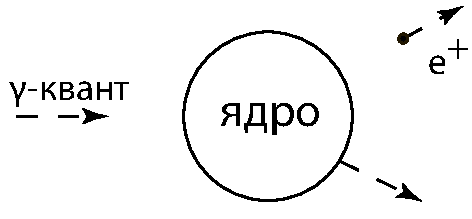
\includegraphics[width=0.47\textwidth]{lec01/save_charge_law_1.pdf}
        }
        \hfill
        \subfigure[Сохранение заряда при аннигиляции]{
            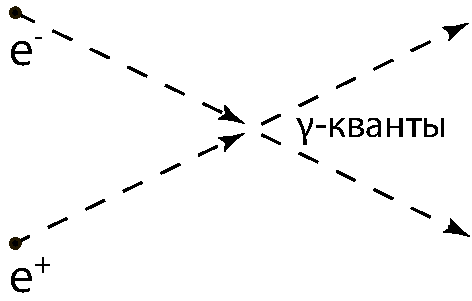
\includegraphics[width=0.47\textwidth]{lec01/save_charge_law_2.pdf}
        }
        \subfigure[Принцип суперпозиции]{
            \begin{tikzpicture}
    \path (-3,0) node[draw,circle] (q1) {$q_1$};
    \path (-2,2) node[draw, circle] (q2) {$q_2$};
    \path (-1,3) node[draw, circle] (q3) {$q_3$};
    \path (1,1)  node[inner sep=.1] (p) {};
    \draw [dashed] (q1) -- (p);
    \draw [dashed] (q2) -- (p);
    \draw [dashed] (q3) -- (p);
    \draw [thick,->] (p) -- (2,1.25);
    \draw [thick,->] (p) -- (2,0.67);
    \draw [thick,->] (p) -- (2,0);
    \draw [thick,->] (p) -- (4,-0.06);
    \node[above] at (2,1.25) {$\vec{F}_{1}$};
    \node[above] at (2,0.67) {$\vec{F}_{2}$};
    \node[above] at (2,0) {$\vec{F}_{3}$};
    \node[above] at (4,-0.06) {$\vec{F}$};
\end{tikzpicture}

        }
        \hfill
        \subfigure[Закон Кулона]{
            \begin{tikzpicture}
    \path (-3,0) node[draw,circle] (q1) {$q_1$};
    \path (3,0) node[draw, circle] (q2) {$q_2$};
    \draw [->] (q1) -- (q2);
    \draw [thick,->] (q1) -- (-4,0);
    \draw [thick,->] (q2) -- (4,0);
    \node[above] at (0,0) {$\vec{r}_{12}$};
    \node[above] at (-4,0) {$\vec{F}_{12}$};
    \node[above] at (4,0) {$\vec{F}_{21}$};
\end{tikzpicture}

        }
        \caption{Свойства электрического заряда}
    \end{figure}
    \begin{enumerate}

        \item установлено, что \textbf{существуют 2 сорта зарядов}: заряды,
        относящиеся к одному из них условно называют положительными, а
        относящиеся к другому -- отрицательными;

        \item установлено, что \textbf{заряды различных сортов притягиваются
        друг другом, а заряды одного и того же сорта -- отталкиваются};

        \item существует \textbf{наименьшая порция электрического заряда}\\
        \(e = 1.6~\cdot~10^{-19}~\text{Кл}\) -- заряд электрона;

        \item частицы протон и электрон имеют элементарные заряды разных
        знаков; условились считать заряд протона положительным, а электрона --
        отрицательным;

        \item \textbf{закон сохранения электрического заряда}: в изолированной
        системе алгебраическая сумма всех зарядов является постоянной
        величиной:
        \[
            \sum\pm q_k = \const;
        \]

        \item \textbf{принцип суперпозиции}: сила взаимодействия заряда с
        группой других равна сумме сил взаимодействий этого заряда с каждым
        зарядом группы;

        \item \textbf{закон Кулона}:
        \begin{equation}
            F = k\frac{q_1q_2}{r^2} \label{eq1:1}
        \end{equation}

    \end{enumerate}


    В СИ единицей измерения заряда является \textit{Кулон} (Кл). По
    определению, \( 1\text{Кл} \) -- это заряд переносимый током
    \( i = 1\text{А} \) за промежуток времени \( \Delta t = 1\text{с} \).

    В системе СИ коэффициент \( k \) определяется следующим образом:
    \[
        k = \frac{1}{4\pi\varepsilon_0},
    \]
    где \( \varepsilon_0 = 8,85\cdot10^{-12} \)~ед. СИ --
    \textbf{электрическая постоянная}.

    Таким образом, в основе электродинамики лежат 3 постулата:
    \begin{enumerate}
        \item закон сохранения заряда;
        \item закон Кулона;
        \item принцип суперпозиции.
    \end{enumerate}



    \begin{figure}[h]
        \center
        \subfigure[Определение электрического поля]{
            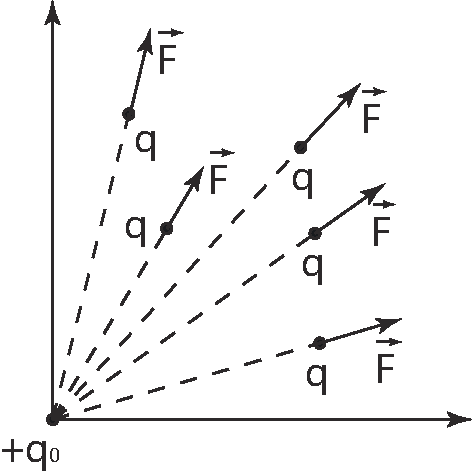
\includegraphics[width=0.30\textwidth]{lec01/electric_field.pdf}
            \label{E_def}
        }
        \hfill
        \subfigure[Напряжённость электрического поля]{
            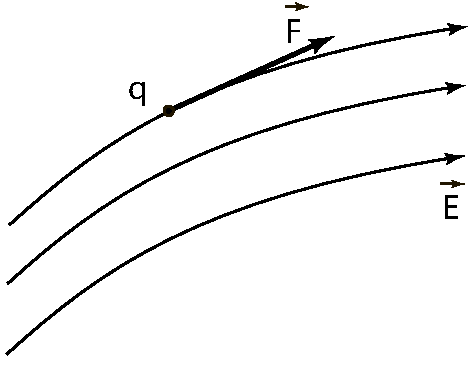
\includegraphics[width=0.30\textwidth]{lec01/E_electric_field.pdf}
        }
        \hfill
        \subfigure[Поле уединённого заряда]{
            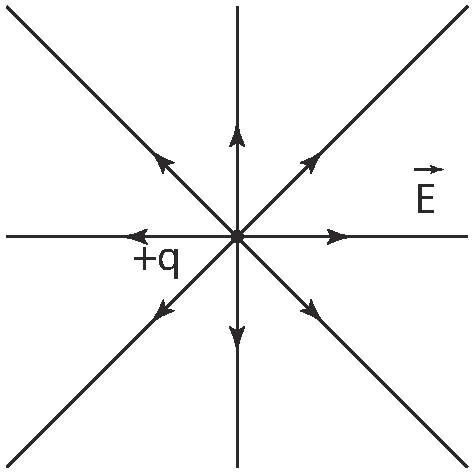
\includegraphics[width=0.30\textwidth]{lec01/field_alone.pdf}
        }
        \hfill
        \subfigure[Поле двух разноимённых зарядов]{
            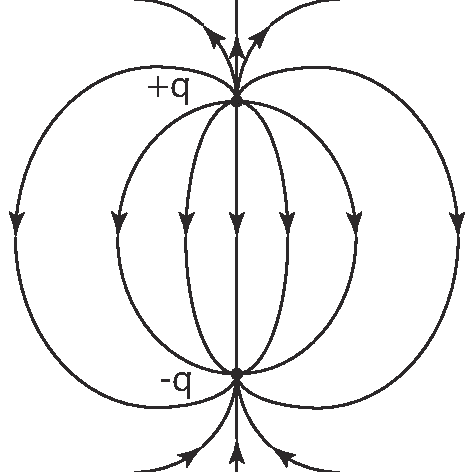
\includegraphics[width=0.47\textwidth]{lec01/field_different.pdf}
        }
        \hfill
        \subfigure[Поле двух одноимённых зарядов]{
            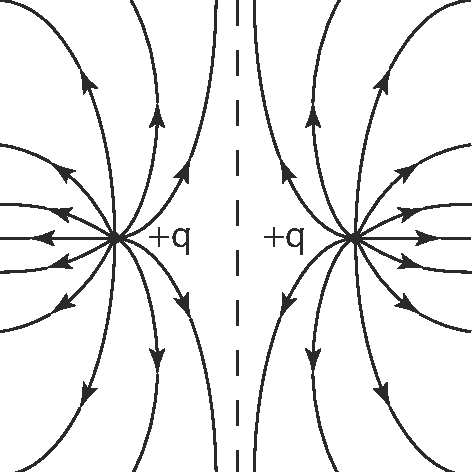
\includegraphics[width=0.47\textwidth]{lec01/field_same.pdf}
        }
        \caption{Электрическое поле}
    \end{figure}

\section{Электрическое поле}
    Поместим точечный заряд \( q_0 \) в начало координат, а другой точечный
    заряд \( q \), называемый пробным, будем помещать то в одной, то в другой
    точке пространства (рис. \ref{E_def}). На заряд в этих точках будет
    действовать сила
    \[
        \vec{F} = k\frac{q_0q}{r^3}\vec{r}
    \]
    Если в каждой точке пространства определена сила, действующая на единичный
    пробный заряд, то говорят, что \textit{задано силовое поле}. Так как эта
    сила имеет электрическое происхождение, то такое силовое поле называется
    \textbf{электрическим}.

    Согласно закону Кулона (\ref{eq1:1}), сила, действующая на точечный заряд
    \( q \), пропорциональна его величине:
    \begin{equation}
        \vec{F} = \vec{E}q\label{eq1:3}
    \end{equation}

    \begin{definition}
        Физическая величина \( \vec{E} \) называется \textbf{напряженностью
        электрического поля} и является его основной силовой характеристикой.
    \end{definition}
    \begin{equation}
        \vec{E}=\frac{\vec{F}}{q} \label{eq1:4}
    \end{equation}

    Из закона Кулона (\ref{eq1:1}) и определения электрического поля
    (\ref{eq1:3}) следует, что напряжённость электрического поля \( \vec{E} \)
    выражается следующим образом:
    \begin{equation}
        \vec{E} = \frac{q}{4\pi\varepsilon_0 r^3}\vec{r} \label{eq1:5}
    \end{equation}

    \begin{definition}
        Если в некоторой области пространства поле \(\vec{E}\) не зависит от
        времени, то оно называется \textbf{постоянным}.
    \end{definition}

    В реальной жизни требуется находить напряжённость поля не одного заряда, а
    группы зарядов. Если мы знаем распределение зарядов в какой-либо области
    пространства, то при помощи принципа суперпозиции  мы можем узнать какую
    напряжённость эта группа зарядов создаёт в окружающем пространстве --
    определить \textbf{электрическое поле}. Однако, аналитически эту задачу
    удаётся решить далеко не всегда. Поэтому, обычно, в задачах на вычисление
    напряжённости рассматриваются симметричные зарядовые конфигурации и
    специфические области пространства.

    \begin{example}
        Найти напряжённость электрического поля \( \vec{E} \) на оси кольца
        радиуса \( R \), равномерно заряженного зарядом \( q \).
    \end{example}

    \begin{figure}[b]
        \center
        \subfigure[Равномерно заряженное кольцо]{
            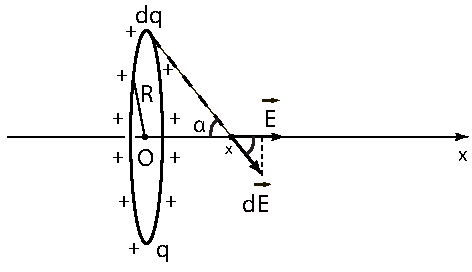
\includegraphics[width=0.47\textwidth]{lec01/ring.pdf}
            \label{1:ring}
        }
        \hfill
        \subfigure[Зависимость \( E(x) \)]{
            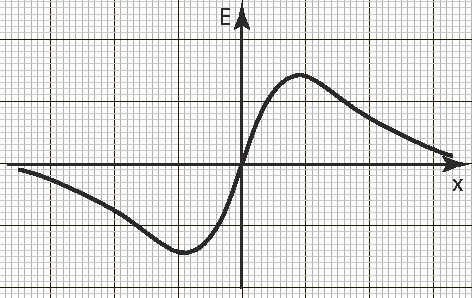
\includegraphics[width=0.47\textwidth]{lec01/E_ring.pdf}
            \label{1:E_ring}
        }
        \caption{К примеру}
    \end{figure}

    \begin{solution}
        Направим вдоль оси кольца ось \( Ox \). В силу симметрии системы,
        результирующая напряжённость \( \vec{E} \) будет направлена вдоль оси
        кольца. Разобьём кольцо на малые участки, несущие заряд \( \dd q \).

        Для нахождения напряжённости нужно, воспользовавшись принципом
        суперпозиции, сложить все проекции на ось \( Ox \) напряжённостей,
        создаваемых в данной точке \( x \) участками \( \dd q \).

        Проекция \( \dd E_x \) напряжённости поля \( \dd\vec{E} \) на ось
        \( Ox \) может быть найдена следующим образом:
        \[
            \dd E_x = \frac{1}{4\pi\varepsilon_0}\cdot
            \frac{\dd q}{R^2+x^2}\cdot\cos\alpha,
        \]
        где угол \( \alpha \) -- это угол между вектором \( \dd\vec{E} \) и
        осью \( Ox \). Из треугольника получим
        \[ \cos\alpha = \frac{x}{\sqrt{R^2+x^2}} \].

        Значение \( E \) найдём проинтегрировав по \( q \) выражение для
        \( \dd E_{x} \):
        \[
            E = \int \dd E_{x} = \frac{x}{4\pi\varepsilon_0\cdot
            (R^2+x^2)^\frac{3}{2}}\cdot\int \dd q =
            \frac{xq}{4\pi\varepsilon_0\cdot(R^2+x^2)^\frac{3}{2}},
        \]
        или в векторном виде
        \[
            \vec{E} = \frac{xq}{4\pi\varepsilon_0\cdot
            (R^2+x^2)^\frac{3}{2}}\cdot\vec{e}_{x}.
        \]

        График этой зависимости изображён на рисунке~\ref{1:E_ring}.
    \end{solution}


    \chapter{Теорема Гаусса}

\section{Теорема Гаусса}
    
    Пусть в пространстве находится группа зарядов \( q_{n} \). Обхватим их 
    поверхностью \( S \). Так как группа зарядов создаёт поле \( \vec{E} \), то 
    через поверхность \( S \) поток поля может быть найден как
    \[
        \Phi = \oiint\limits_S \vec{E}\cdot\dd\vec{S}.
    \]
    Рассмотрим теорему, связывающую поток поля \( \vec{E} \) через замкнутую 
    поверхность \( S \) с зарядом, находящимся внутри поверхности.
    
    \begin{figure}[b]
        \center
        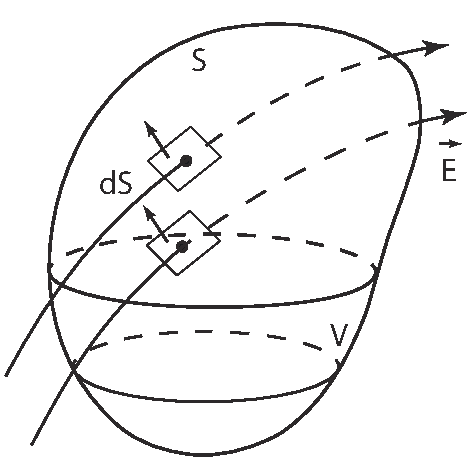
\includegraphics[width=0.30\textwidth]{lec02/flux_E.pdf}
        \hfill
        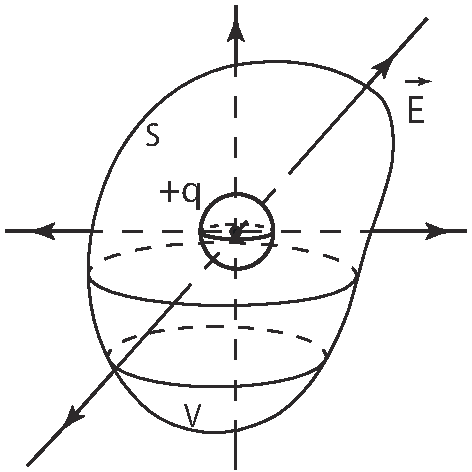
\includegraphics[width=0.30\textwidth]{lec02/Gauss_theorem.pdf} 
        \hfill
        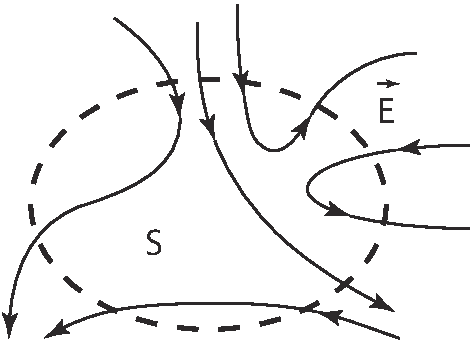
\includegraphics[width=0.30\textwidth]{lec02/Earnshaw_theorem.pdf}
        \parbox[t]{.3\textwidth}{
            \caption{Поток поля Е через поверхность S}
        }
        \hfill
        \parbox[t]{.3\textwidth}{
            \caption{К доказательству теоремы Гаусса}
        }
        \hfill
        \parbox[t]{.3\textwidth}{
            \caption{К доказательству теоремы Ирншоу}
        }
    \end{figure}
    

    \begin{theorem}[Гаусс]
        Поток поля \( \vec{E} \) через произвольную замкнутую поверхность
        \( S \) равен алгебраической сумме зарядов внутри \( S \), отнесённый к 
        \( \Ezero \), и не зависит ни от конфигурации зарядов, ни от формы
        \( S \).
        \begin{equation}
            \label{eq:thegauss}
            \Phi = \oiint\limits_S \vec{E}\cdot\dd\vec{S} = 
            \frac{\sum{q}}{\Ezero} = \frac{q_{S}}{\Ezero}
        \end{equation}
    \end{theorem}


    \begin{proof}
        Докажем сначала для одного заряда, затем применим принцип суперпозиции. 
        Так как заряд \( q \) является точечным изолированным источником поля 
        \( \vec{E} \), то, в силу следствия 2 теоремы Остроградского поток 
        через произвольную поверхность будет равен потоку через сферу радиуса 
        \( R \) в центре которой расположен заряд \( q \):
        \[
            \oiint\limits_S \vec{E}\cdot\dd\vec{S} = 
            \oiint\limits_{4\pi R^{2}} \vec{E}\cdot\dd\vec{S} = 
            \oiint\limits_{4\pi R^{2}}\frac{\vec{r}\cdot\dd\vec{S}}{r^3}
            \cdot\frac{q}{4\pi\Ezero}.
        \]

        А так как на сфере \( \vec{r} \uparrow\uparrow \dd\vec{S} \) и
        \( r = \const = R\), то
        \[
            \oiint\limits_{4\pi R^{2}}
            \frac{\vec{r}\cdot\dd\vec{S}}{r^3}\cdot\frac{q}{4\pi\Ezero} = 
            \frac{q}{4\pi\Ezero}\oiint\limits_{4\pi R^2} \frac{R\dd S}{R^3} = 
            \frac{q}{4\pi\Ezero R^2}\oiint\limits_{4\pi R^2}\dd S = 
            \frac{q}{\Ezero}.
        \]

        Если \( q \) лежит вне поверхности \( S \), то внутри \( S \)
        \( \div\vec{E} \equiv 0 \) и
        \[
            \Phi_{S} = \oiint\limits_S \vec{E}\cdot\dd\vec{S} = 
            \iiint\limits_V \div\vec{E}\dd V = 0.
        \]

        Итак, если внутри \( S \) содержится много зарядов, то в силу принципа 
        суперпозиции:

        \[
            \vec{E}=\sum\limits_k \vec{E}_{k},
        \]
        \[
            \Phi_{S} = \oiint\limits_S \vec{E}\cdot\dd\vec{S} =
            \sum\limits_k\oiint \vec{E}_{k}\cdot\dd \vec{S} =
            \sum\limits_k \frac{\pm q_{k}}{\Ezero} = \frac{q_{S}}{\Ezero}.
        \]

    \end{proof}

    Если заряд распределён в пространстве непрерывно, то
    \[
        q_{S} = \iiint\limits_V \rho(x,y,z)\dd V ,
    \]
    где \( \rho \) -- объёмная плотность заряда. Тогда теорема Гаусса даёт
    \[
        \oiint\limits_S \vec{E}\cdot\dd\vec{S} =             
        \frac{1}{\Ezero}\iiint\limits_V\rho\dd V,
    \]
    но, по теореме Остроградского,
    \[
        \oiint\limits_S \vec{E}\cdot\dd\vec{S} =
        \iiint\limits_V \div\vec{E}\dd V,
    \]
    таким образом,
    \[ 
        \iiint\limits_V \div\vec{E}\dd V =
        \frac{1}{\Ezero}\iiint\limits_V \rho\dd V,
    \]
    а так как область \( V \) произвольна, то подынтегральные значения равны:
    \begin{equation}
        \label{eq:thegaussdiff}
        \div\vec{E} = \frac{\rho}{\Ezero}.
    \end{equation}

    Формула (\ref{eq:thegaussdiff}) -- это дифференциальный вид
    (\ref{eq:thegauss}), она связывает поле \( \vec{E} \) и заряд в данной 
    точке.

\section{Теорема Ирншоу}

    \begin{theorem}[Ирншоу]
        Равновесие зарядов в электростатическом поле не может быть устойчивым.
    \end{theorem}

    \begin{proof}
        Пусть в поле \( \vec{E} \), созданном какими-либо внешними зарядами, 
        есть область устойчивости \( S \). Отсюда следует, что все линии 
        стабилизирующего поля \( \vec{E} \) входят в \( S \), но, так как в 
        области \( S \) зарядов нет, то, по теореме Гаусса,
        \[
            \oiint\limits_S \vec{E}\cdot\dd\vec{S} = 0,
        \]
        то есть сколько линий входит, столько и выходит. Таким образом 
        существуют траектории, выходящие за пределы области \( S \), движение 
        вдоль которых энергетически выгодно для заряда, находящегося в 
        состоянии равновесия в области, то есть его положение равновесия не 
        является устойчивым.
    \end{proof}

\section{Применение теоремы Гаусса}
    \begin{figure}[b]
        \center
        \subfigure[Поле плоскости]{
        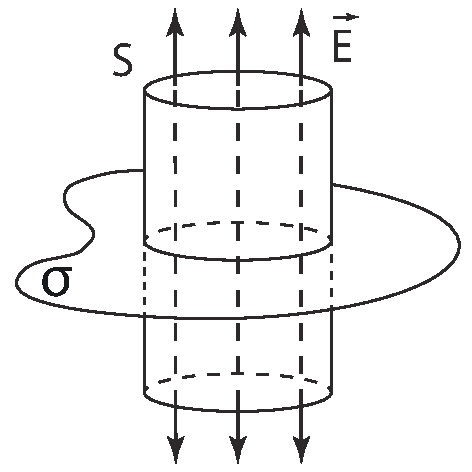
\includegraphics[width=0.30\textwidth]{lec02/plane_field.pdf} 
        \label{E_def}
        }
        \subfigure[Поле нити]{
        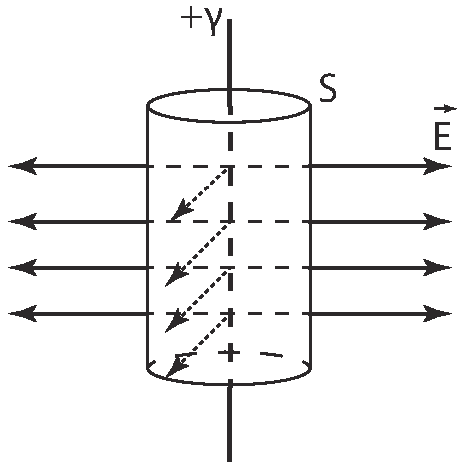
\includegraphics[width=0.30\textwidth]{lec02/thread_field.pdf}
        }
        \subfigure[Поле сферы]{
        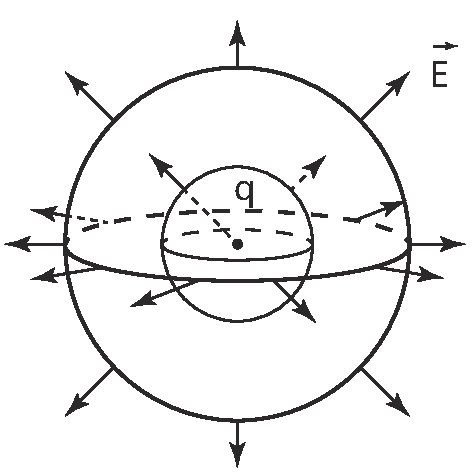
\includegraphics[width=0.30\textwidth]{lec02/sphere_field.pdf}
        }    
        \caption{Электрическое поле}
    \end{figure}
    
    \begin{figure}[b]
        \center
        \subfigure[Поле плоскости]{
            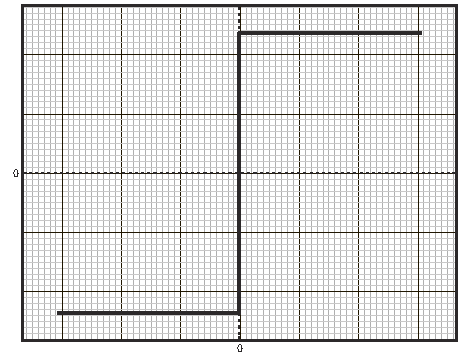
\includegraphics[width=0.3\textwidth]{lec02/plane_field_plot.pdf}
            \label{plane_field_plot}
        }
        \subfigure[Поле нити]{
            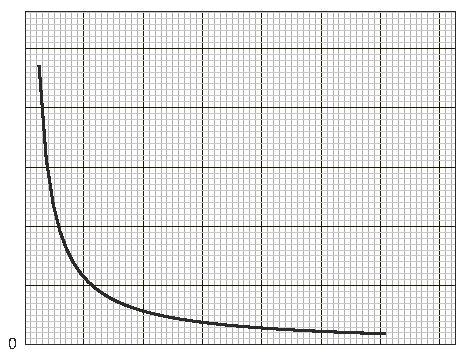
\includegraphics[width=0.30\textwidth]{lec02/thread_field_plot.pdf}
            \label{thread_field_plot}
        }
        \subfigure[Поле сферы]{
            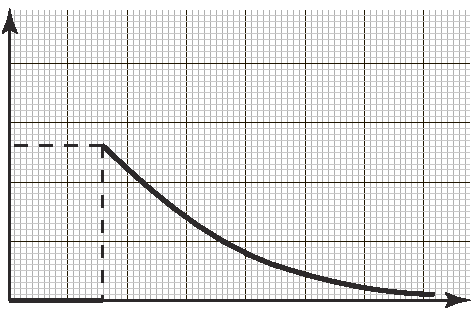
\includegraphics[width=0.30\textwidth]{lec02/sphere_field_plot.pdf}
            \label{sphere_field_plot}
        }
        \caption{Зависимости напряжённости поля от расстояния до системы}
    \end{figure}
    
    Теорема Гаусса, вообще говоря, не позволяет вычислить поле \( \vec{E} \) 
    заданной произвольной конфигурации зарядов, так как из знания интеграла 
    \( \Phi_S \) не следует знание \( \vec{E}(x,y,z) \). Однако, для некоторых 
    симметричных зарядовых конфигураций \( \Phi_S \sim ES \) и тогда теорема 
    Гаусса помогает считать значительно быстрее. 

    \begin{example}
        Вычислить поле \(\vec{E}\) бесконечной плоскости, на которой заряд 
        распределён равномерно с поверхностной плотностью
        \( \sigma\ (\text{Кл}/\text{м}^2) \).
    \end{example}


    \begin{solution}
        В силу симметрии объекта, поле \( \vec{E} \) плоскости может быть 
        только перпендикулярно плоскости. Поэтому найдём такое поле
        \( \vec{E} \).

        Обернём плоскость замкнутой поверхностью \( S \) в виде цилиндра, 
        перпендикулярного плоскости.
        \[
            S = S_{\textit{бок}} + 2S_{\textit{тор}}.
        \]

        Тогда, по теореме Гаусса,
        \[
            \oiint\limits_S \vec{E}\cdot\dd\vec{S} = \frac{q_{S}}{\Ezero},
        \]
        где \( q_{S} = \sigma\cdot S_{\textit{тор}} \) (заряд, вырезанный
        \( S \)).

        \[
            \Phi = \iint\limits_{S_{\textit{бок}}} \vec{E}\cdot\dd\vec{S} +
            2\iint\limits_{S_{\textit{тор}}} \vec{E}\cdot\dd\vec{S} =         
            2ES_{\textit{тор}}
        \]

        Таким образом,
        \[ 
            2ES_{\textit{тор}} = \frac{\sigma S_{\textit{тор}}}{\Ezero}
            \Rightarrow E = \frac{\sigma}{2\Ezero}
        \].

    \end{solution}

    \begin{example}
        Вычислить поле \( \vec{E} \) прямой бесконечной нити, равномерно 
        заряженной с погонной (линейной) плотностью
        \( \gamma\ (\text{Кл}/\text{м}) \).
    \end{example}

    \begin{solution}
        Охватим участок нити длины \( h \) соосным цилиндром радиуса \( r \). 
        Его площадь
        \[
            S = S_{\textit{бок}} + 2S_{\textit{тор}}.
        \]
        
        Так как поток поля через торцы равен 0 и
        \( \vec{E} \uparrow\uparrow \dd\vec{S} \), \( \vec{E} = \const \) на
        \( S_{\textit{бок}} \), то 
        \[
            \iint\limits_{S_{\textit{бок}}} \vec{E}\cdot\dd\vec{S} = 
            E\iint\limits_{S_{\textit{бок}}} \dd S = E\cdot 2\pi rh
        \]

        А так как цилиндр вырезает заряд \( q_{S} = \gamma h \), то, по теореме 
        Гаусса:
        \[
            E\cdot 2\pi rh = \frac{\gamma h}{\Ezero} \Rightarrow E = 
            \frac{\gamma}{2\pi\Ezero r}.
        \]
        В декартовых координатах:
        \[
            \vec{E}=\frac{\gamma}{2\pi\Ezero(x^2+y^2)}\cdot \{x, y, 0\}.
        \] 
    \end{solution}
    \begin{example}
        Вычислить поле \( \vec{E} \) сферы радиуса \( R \),
        несущей заряд \( q \).
    \end{example}
    \begin{solution}
        Сфера разделяет пространство на 2 части: внутреннюю и внешнюю по 
        отношению к сфере.
        \begin{enumerate}
        \item \( | \vec{r} | < R \) (внутри сферы).
            
            \( E_{in} \equiv 0 \), так как внутри любой сферической поверхности
            \( 4\pi r^2 \) (\( r < R \)) заряд \( q = 0 \).
            \[ \oiint\limits_{4\pi R^2} \vec{E}\cdot\dd\vec{S} = 0 \]

        \item \( | \vec{r} | > R \) (вне сферы).
      
            \[
                \oiint\limits_{4\pi R^2} \vec{E}\cdot\dd\vec{S} = 
                \frac{q_{S}}{\Ezero} = \frac{q}{\Ezero}.
            \]
            С другой стороны,
            \[
                \oiint\limits_{4\pi R^2} \vec{E}\cdot\dd\vec{S} =
                E_{ex}\cdot S_\textit{сф} =
                4\pi R^2 E_{ex} \Rightarrow \text{ при \( r > R\): }
                E = \frac{q}{4\pi\Ezero r^2}
            \]
        \end{enumerate} 

        Таким образом,
        \[ E = \frac{q}{4\pi\Ezero r^2} \].

        График этой зависимости изображён на рисунке~\ref{sphere_field_plot}.
        
    \end{solution}

    \chapter{Потенциал}

\section{Теорема о циркуляции поля \textbf{E}}
    
    \begin{theorem}
        Циркуляция электростатического поля \( \vec{E} \) равна нулю, то есть
        \begin{equation}
            \oint\limits_C \vec{E}\cdot\dd\vec{l} = 0. \label{eq3:1}
        \end{equation}
    \end{theorem}
    
    \begin{proof}
        Есть два способа доказательства:
        \begin{enumerate}
            \item Вычислим работу поля
                \[
                    \vec{E} = \frac{q}{4\pi\varepsilon_0 r^2}
                \]
                одиночного точечного заряда \( q \) от точки 1 до точки 2:
                
                \[ 
                    A_{1\to2} = \int\limits_{1}^{2} \vec{E}\cdot\dd\vec{l} =
                    \int\limits_{1}^{2} E \dd l \cos\alpha =
                    \int\limits_{1}^{2} \frac{q}{4\pi\varepsilon_0 r^2}\dd r =
                    \frac{q}{4\pi\varepsilon_0}\left(\frac{1}{r_1} -
                    \frac{1}{r_2}\right)
                \]
            
            \item (см. Тензорный анализ 6.1.2 - 2)
                Так как 
                \[
                    \vec{E} = \frac{q}{4\pi\varepsilon_0}\cdot
                    \frac{\vec{r}}{r^3},
                \] 
                то
                \begin{align*}
                    & \int\limits_1^2 \vec{E}\cdot\dd\vec{l} =
                    \frac{q}{4\pi\varepsilon_0} \int\limits_1^2
                    \frac{xdx + ydy + zdz}{r^3} =
                    \frac{q}{4\pi\varepsilon_0}\cdot\frac{1}{2}\int\limits_1^2
                    \frac{\dd(x^2+y^2+z^2)}{r^3} = \\ = &
                    \frac{q}{4\pi\varepsilon_0} \int\limits_1^2 
                    \frac{r}{r^3}\dd r =
                    \frac{q}{4\pi\varepsilon_0}\left(\frac{1}{r_1} - 
                    \frac{1}{r_2}\right).
                \end{align*}
        \end{enumerate}
        Видно, что результат не зависит от формы пути, а только от 
        координат начальной и конечной точек.
        
        В частности, если \( \vec{r}_1 = \vec{r}_2 \), то есть кривая 
        образует замкнутый контур \( C \), то
        \[
            \oint\limits_C \vec{E}\cdot\dd\vec{l} = 0.
        \]
        
        Если поле \( \vec{E} \) образовано группой зарядов, то, в силу 
        принципа суперпозиции,
        \[ 
            \vec{E} = \sum\limits_k \vec{E}_{k},
        \]
        \[
            \oint\limits_C \vec{E}\cdot\dd\vec{l} =
            \sum\limits_k \oint\limits_{C_k}
            \vec{E}_{k}\cdot\dd\vec{l} = 0.
        \]
        
        Таким образом, для \( \vec{E} \):
        \[
            \oint\limits_C \vec{E}\cdot\dd\vec{l} = 0.
        \]
        
    \end{proof}
    
    \begin{definition}
        Всякое поле, циркуляция по контуру которого равна 0, является     
        \textbf{потенциальным}.
    \end{definition}
    
    Таким образом, \( \vec{E} \) -- потенциальное. По теореме Стокса:
    \[
        \oint\limits_C \vec{E}\cdot\dd\vec{l} = \iint\limits_S 
        \rot\vec{E}\cdot\dd\vec{S} \Rightarrow \rot\vec{E} = 0
        \text{, т.е. поле \( \vec{E} \) -- безвихревое}
    \]
    
    Получаем основные уравнения электростатики, которые вы можете видеть в 
    таблице \ref{fund_eq_e}. 
    
    \begin{table}[ht]
        \center
        \caption{Основные уравнения электростатики} \label{fund_eq_e}
        \begin{tabular}[ht]{|c|c|c|c|} \hline
            Название & \( \int \)-форма & \( \dd \)-форма & Смысл \\ \hline
            %------------------------------------------------------------
            & & & \\ % dirty hack for vertical space
            Теорема Гаусса & \( \oiint\limits_S\vec{E}\cdot\dd\vec{S}    
            =\frac{q_{S}}{\Ezero} \) & \( \div\vec{E}=\frac{\rho}{\Ezero} \)
            & поле \( \vec{E} \) рождается в источниках (\( \rho \)) \\
            %------------------------------------------------------------
            Теорема о циркуляции & \( \int\limits_C\vec{E}\cdot\dd\vec{l}=0 \) 
            & \( \rot\vec{E}=0 \) & поле \( \vec{E} \) - потенциально \\ \hline
            %------------------------------------------------------------
        \end{tabular}
    \end{table}
    
    \begin{remark}
        Линии поля \( \vec{E} \) \textit{не могут} быть замкнутыми, так как 
        выбрав контур по этой линии, то есть 
        \( \dd\vec{l} \uparrow\uparrow \vec{E} \) в каждой точке, получим 
        \[
            \oint\limits_C \vec{E}\cdot\dd\vec{l} = \oint\limits_{C} E\dd l > 0,
        \]
        что противоречит (\ref{eq3:1}).
    \end{remark}
    
\section{Потенциал и разность потенциалов}
    
    Так как \( \vec{E} \) -- потенциально, то его работа от точки 1 до точки 2:
    \[
        A_{1\to2} = \int\limits_1^2 \vec{E}\cdot\dd\vec{l} =
        \varphi_1 - \varphi_2,
    \]
    где \( \varphi_1,\ \varphi_2 \) -- функции координат точек 1 и 2 
    соответственно, и не зависит от формы кривой \( 1 \rightarrow 2 \).
    
    Чтобы определить \( \varphi \) поля \( \vec{E} \) как однозначную функцию 
    координат точки: \( \varphi = \varphi(x, y, z) \), обычно делают так:
    \begin{itemize}
        \item фиксируют точку 2 в качестве базовой точки \(M_0(x_0, y_0, z_0)\);
        \item полагают \( \varphi(M_0) = 0 \);
        \item точку 1 берут в качестве \( M(x, y, z) \), в которой и определяют 
            потенциал.
    \end{itemize}
    
    Если заряд (или группа зарядов) уединён, то \( M_0 \) - лежит на 
    бесконечности и \( \varphi(M_0) = 0 \). Если заряд распределён по 
    бесконечному объекту, то ни в нуле, ни в бесконечности
    \( \varphi(M_0) \ne 0 \).
    
    Итак, для ограниченных объектов поток их поля:
    \[
        \varphi(M) = \int\limits_M^{\infty} \vec{E}\cdot\dd\vec{l}
        \text{\ по любому пути}.
    \]
    
    Последнее уравнение -- это работа по перемещению заряда из данной точки в 
    бесконечность.
    
    \begin{definition}
        Выражение
        \[
            \Delta\varphi = \varphi_2 - \varphi_1 = \int\limits_1^2 
            \vec{E}\cdot\dd\vec{l}
        \]
        называется \textbf{разностью потенциалов} между точками 1 и 2 в поле
        \( \vec{E} \), а функция \( \varphi \) -- \textbf{потенциалом}.
    \end{definition}
    
    Размерность:
    \[
        [\varphi] = [\Delta\varphi] = \text{В},
    \]
    \[
        E = \frac{\varphi}{l} = \frac{\text{В}}{\text{м}}.
    \]
    
    Из принципа суперпозиции для \( \vec{E} \) следует свойство аддитивности 
    потенциалов: потенциал группы зарядов равен алгебраической сумме 
    потенциалов отдельных зарядов:
    \[
        \varphi = \sum\limits_k \pm \varphi_{k}.
    \]
    
    Итак, потенциал
    \begin{equation}
        \label{eq3:2}
        \varphi_{M} = \int\limits_M^{\infty} \vec{E}\cdot\dd\vec{l}
    \end{equation}
    Домножим (\ref{eq3:2}) на \( q \), получим    
    \[
        q\varphi_{M} = \int\limits_M^{\infty} q\vec{E}\cdot\dd\vec{l};
    \]
    а так как по определению \( \vec{E} = \frac{\vec{F}}{q} \), то
    \[
        q\varphi_{M} = \int\limits_M^{\infty} \vec{F}\cdot\dd\vec{l} =
        A_{M \rightarrow \infty}
    \]
    есть работа поля \( \vec{E} \) по переносу заряда \( q \) от точки \( M \)
    на \( \infty \).

    А так как \( A_{M \rightarrow \infty} \) в потенциальном поле равна 
    потенциальной энергии частицы \( W \) в точке \( M \), то 
    \[
        \varphi_{M} = \frac{W}{q} \left(\frac{\text{Дж}}{\text{Кл}} =
        \text{В}\right)
    \]
    
    Таким образом, потенциал точки \( M \) равен 1В, если заряд \( q = 1\)Кл 
    обладает в точке \( M \) энергией 1Дж.
    
    \begin{remark}
        В физике используется малая внесистемная единица энергии электрон-вольт 
        (эВ).
        
        По определению, 1эВ -- энергия заряда
        \( q = 1e = 1,6 \cdot 10^{-19} \)~Кл в точке поля
        \( \varphi = 1 \)~В (или ускоренного таким потенциалом).
        
        \[
            W = 1\text{эВ} = 1,6 \cdot 10^{-19}\text{Кл\( \cdot \)В} =
            1,6 \cdot 10^{-19}\text{ Дж}.
        \]
    \end{remark}
    
\section{Вычисление потенциалов}

    \begin{example}
        Найти потенциал точечного заряда \( q \).
    \end{example}
    
    \begin{solution}
        Так как путь можно выбирать любой, то пойдём в \( \infty \) по \( 
        \vec{r} \): \( \dd\vec{l} = \dd\vec{r} \).
        \[
            \vec{E} = \frac{q}{4\pi\varepsilon_0 r^3} \vec{r},
        \]
        \[
            \varphi(r) = \int\limits_r^{\infty} E(r)\dd r = 
            \frac{q}{4\pi\varepsilon_0} \int\limits_r^{\infty}
            \frac{1}{r^2}\dd r = \frac{q}{4\pi\epsilon_0 r}.
        \]
    \end{solution}
    
    \begin{example}
        Определить распределение потенциала поля заряженной сферы радиуса
        \( R \), несущей заряд \( q \).
    \end{example}
    
    \begin{figure}[!b]
        \center
        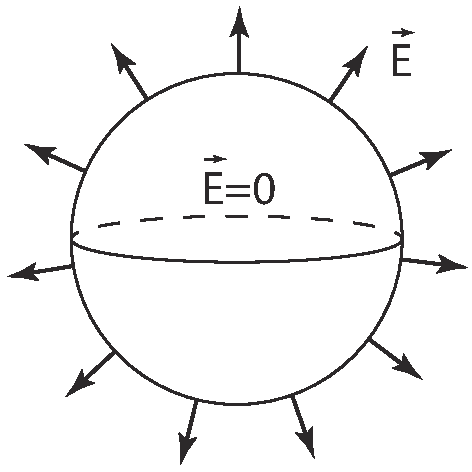
\includegraphics[width=.47\textwidth]{lec03/sphere.pdf}
        \hfill
        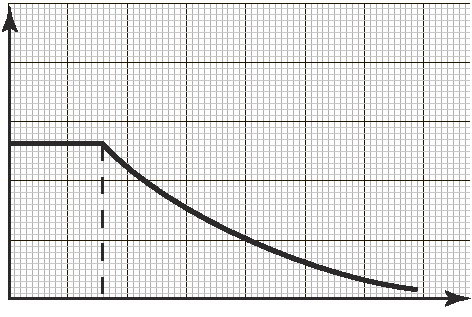
\includegraphics[width=0.47\textwidth]{lec03/sphere_plot.pdf}
        \parbox[t]{.47\textwidth}{\caption{Заряженная сфера}\label{3:sphere}}
        \hfill
        \parbox[t]{.47\textwidth}{\caption{Потенциал заряженной сферы}
        \label{3:sphere_plot}}
    \end{figure}
    
    \begin{solution}
        Сфера представлена на рисунке~\ref{3:sphere}. Как и в прошлый раз, 
        разобъём задачу на 2 подзадачи:
    \begin{enumerate}
        \item \( r > R \):        
            
            Так как поле сферы при \( r > R \)
            \[
                E = \frac{q}{4\pi\varepsilon_0 r^2},
            \]
            а работа потенциального поля не зависит от формы пути, то уходим в 
            бесконечность по радиусу:
            \[
                \varphi(r) = \int\limits_r^{\infty} E(r)\dd r = 
                \frac{q}{4\pi\varepsilon_0 r}
            \]
        \item \( r < R \):
        
            Идём по двум этапам:
            \[
                \varphi(r) = \int\limits_r^R E_{\textit{внутр}}(r)\dd r + 
                \int\limits_R^{\infty} E_{\textit{внеш}}(r)\dd r = 
                \frac{q}{4\pi\varepsilon_0 R} = \const
            \]
            График распределения потенциала сферы \( \varphi (r) \) представлен 
            на рисунке~\ref{3:sphere_plot}.
    \end{enumerate}
    \end{solution}
    
    \begin{example} % picture here or somewhere
        Вычислить разность потенциалов между точками 1 и 2 в  поле нити, 
        заряженной \( e \) с погонной плотностью \( \gamma \).
    \end{example}
    
    \begin{solution}
    Так как \( \Delta\varphi_{1 \to 2} \) не зависит от формы пути, то выбираем 
    путь так: \( 1 \to 2 = 1 \to 1’ + 1’ \to 2 \).
    \[
        \Delta\varphi_{1 \to 2} = \int\limits_1^{1’} \vec{E}\cdot\dd\vec{l} + 
        \int\limits_{1’}^2 \vec{E}\cdot\dd\vec{l}
    \]
    
    Так как \( \vec{E} \uparrow\uparrow \dd\vec{l}_{1 \to 1’} \) и
    \( \vec{E} \perp \dd\vec{l}_{1’ \to 2} \), то
    \[
        \Delta\varphi_{1 \to 2} = \int\limits_{r_1}^{r_2} 
        \frac{\gamma}{2\pi\varepsilon_0 r}\dd r = 
        \frac{\gamma}{2\pi\varepsilon_0}\ln{\frac{r_2}{r_1}}
    \]
    \end{solution}
    
    \begin{figure}[b]
        \center
        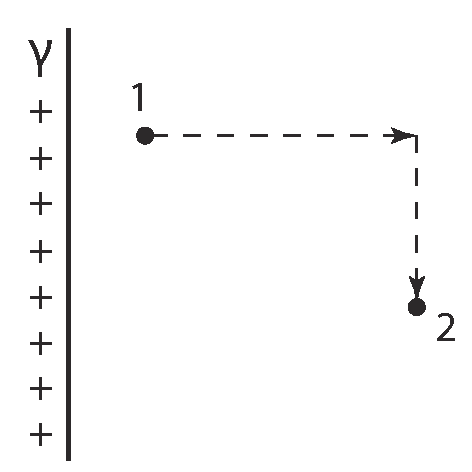
\includegraphics[width=.3\textwidth]{lec03/thread_field.pdf}
        \hfill
        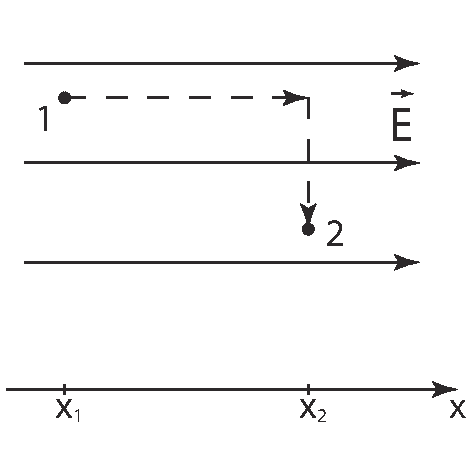
\includegraphics[width=.3\textwidth]{lec03/plane_field.pdf}
        \hfill
        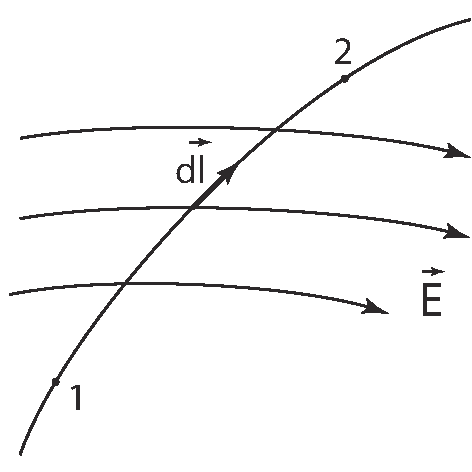
\includegraphics[width=.3\textwidth]{lec03/potential.pdf}
        \parbox[t]{.3\textwidth}{\caption{К вычислению потенциала поля заряженной нити}}
        \hfill
        \parbox[t]{.3\textwidth}{\caption{Разность потенциалов в однородном поле}}
        \hfill
        \parbox[t]{.3\textwidth}{\caption{Связь напряженности поля с его потенциалом}}
    \end{figure}

    \begin{example} % picture here or somewhere near
        Определить разность потенциалов между точками 1 и 2 в поле
        \( \vec{E} = \const \).
    \end{example}
    
    \begin{solution}
    Так как \( \Delta\varphi_{1 \to 2} \) не зависит от формы пути, то выбираем 
    путь так: \( 1 \to 2 = 1 \to 1’ + 1’ \to 2 \).
    \[
        \Delta\varphi_{1 \to 2} = \int\limits_1^{1’} \vec{E}\cdot\dd\vec{l} + 
        \int\limits_{1’}^2 \vec{E}\cdot\dd\vec{l} = E \Delta x = E(x_2 - x_1)
    \]
    \end{solution}

\section{Выражение поля \textbf{E} через заданное распределение потенциала}

    Формула (\ref{eq3:2}) даёт выражение \( \varphi (x, y, z) \) через заданное 
    поле \( \vec{E} (x, y, z) \).
    Поставим обратную задачу: как найти \( \vec{E} (x, y, z) \) через
    \( \varphi (x, y, z) \)?
    
    \begin{solution} % funky picture again.
    Выделим на кривой \( L \) в поле \( \vec{E} \) две близкие точки 1 и 2.
    \[
        \varphi_2 = \varphi_1 + \Delta\varphi \Rightarrow 
        \vec{E}\cdot\dd\vec{l} = \varphi_1 - \varphi_2 = -\dd\varphi = -
        \left(\partder{\varphi}{x}\dd x + \partder{\varphi}{y}\dd y + 
        \partder{\varphi}{z}\dd z\right) = -\nabla\varphi\cdot\dd\vec{l} \]
    
    Таким образом,
    \[
        \vec{E}\cdot\dd\vec{l} = -\nabla\varphi\cdot\dd\vec{l},
    \]
    но, так как \( \dd\vec{l} \) -- любой произвольный отрезок, то 
    \begin{equation}
        \label{eq3:3}
        \vec{E} = -\nabla\varphi
    \end{equation}
    А компоненты поля \( \vec{E} \) имеют следующий вид:
    \begin{align*}
        & E_{x} = -\partder{\varphi}{x},\\
        & E_{y} = -\partder{\varphi}{y},\\
        & E_{z} = -\partder{\varphi}{z}
    \end{align*}
    \end{solution}
    
\section{Эквипотенциальные поверхности}
    \begin{figure}[b!]
        \center
        \subfigure[Поле одноимённых зарядов]{
        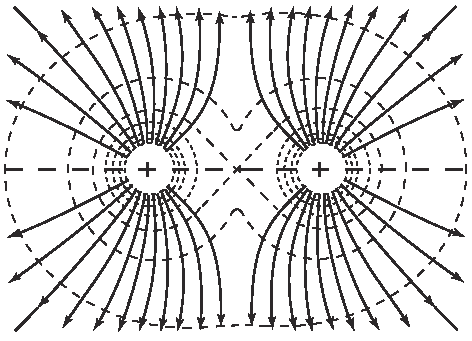
\includegraphics[width=0.47\textwidth]{lec03/equipot_same.pdf}}
        \subfigure[Поле разноимённых зарядов]{
        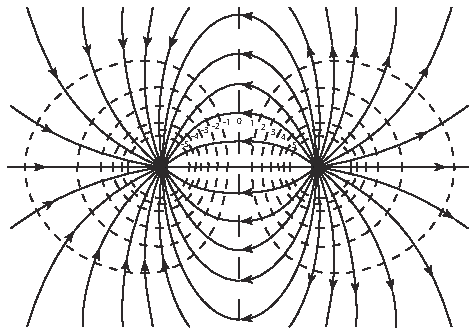
\includegraphics[width=0.47\textwidth]{lec03/equipot_different.pdf}}
        \caption{Эквипотенциали}
    \end{figure}

    \begin{definition}
        \textbf{Эквипотенциальные поверхности} -- это поверхности в пространстве, 
        на которых \( \varphi (x, y, z) = \const \), то есть эквипотенциали --  
        это поверхность уровня поля \( \varphi (x, y, z) \). 
    \end{definition}
    
    Так как \( \vec{E} = -\nabla\varphi \), и вектор \( \nabla\varphi \) 
    перпендикулярен к поверхности, на которой \( \varphi = \const \), то и 
    линии поля \( \vec{E} \) перпендикулярны к ней.

    Таким образом. семейства линий \( \vec{E} \) и эквипотенциальные 
    поверхности везде взаимно перпендикулярны.
    
\section{Электрический диполь}

    Электрический диполь -- это пара одинаковых зарядов \( +q \) и \( -q \), 
    разнесённых  на расстояние \( l \). Дипольный момент диполя равен 
    \[
        \vec{p} = q\vec{l},
    \]
    где \( l \) -- длина диполя.

    \begin{figure}[b]
        \center
        \subfigure[Молекула воды]{
        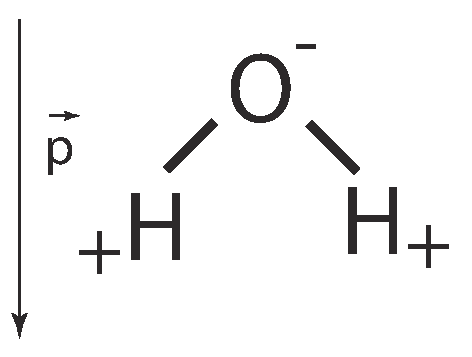
\includegraphics[width=0.18\textwidth]{lec03/water.pdf}}
        \subfigure[Молекула кислорода]{
        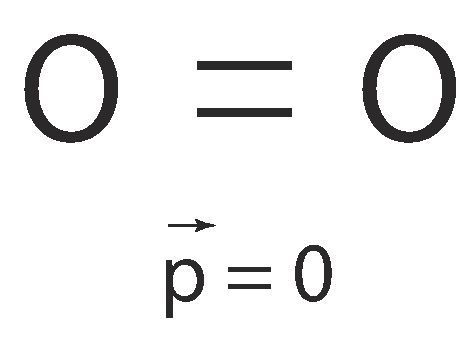
\includegraphics[width=0.18\textwidth]{lec03/oxygen.pdf}}
        \subfigure[Молекула озона]{
        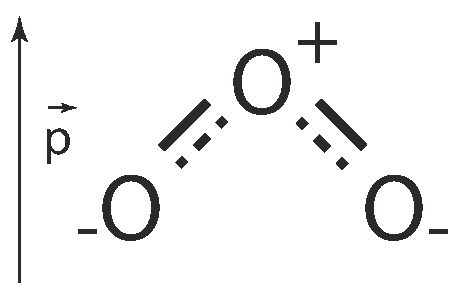
\includegraphics[width=0.18\textwidth]{lec03/ozone.pdf}}
        \subfigure[Молекула аммиака]{
        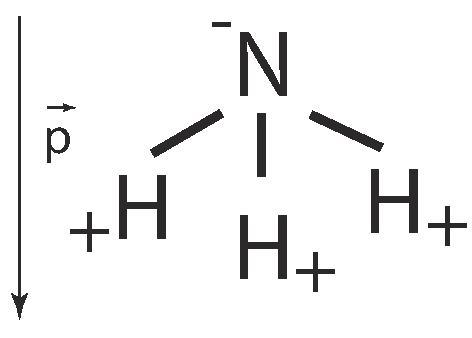
\includegraphics[width=0.18\textwidth]{lec03/ammonia.pdf}}
        \subfigure[Молекула метана]{
        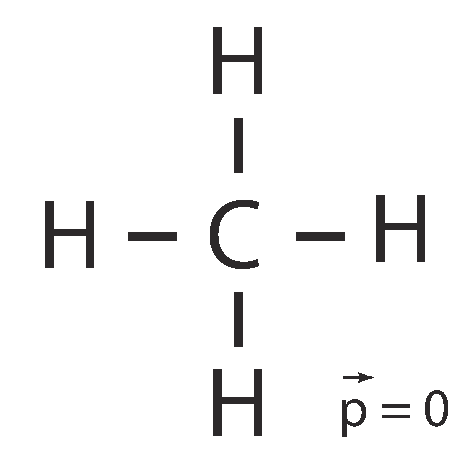
\includegraphics[width=0.18\textwidth]{lec03/methane.pdf}}
        \caption{Дипольные моменты молекул}
    \end{figure}   

    Зачастую, молекулы веществ являются диполями:   
    \begin{itemize}
        \item молекула воды \( H_2O \),
        \item молекула озона \( O_3 \),
        \item молекула аммиака \( NH_3 \).
    \end{itemize}

    Диполь называется точечным, если расстояние, с которого оценивается его 
    действие, много больше длины диполя.
    
\subsection{Потенциал и поле точечного диполя}

    \begin{figure}[b]
        \center
        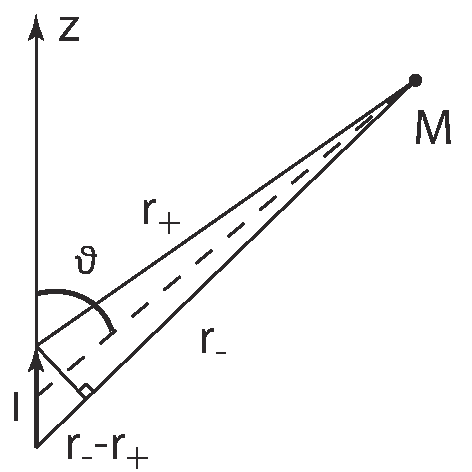
\includegraphics[width=.47\textwidth]{lec03/dipole_calculate.pdf}
        \hfill
        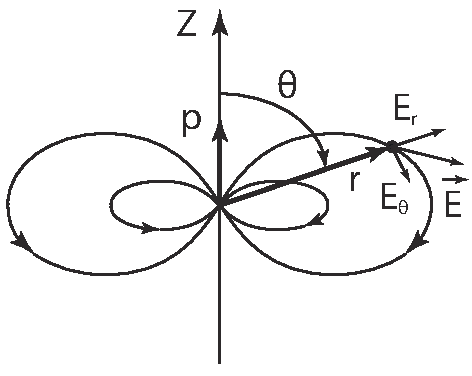
\includegraphics[width=.47\textwidth]{lec03/dipole_field.pdf}
        \parbox[t]{.47\textwidth}{\caption{Вычисление потенциала поля диполя}}
        \hfill
        \parbox[t]{.47\textwidth}{\caption{Поле диполя}}
    \end{figure}

    Вычислим потенциал и поле точечного диполя. Из свойства аддитивности
    потенциала следует:
    \[
        \varphi = \varphi_{+} + \varphi_{-}
    \]
    Или:
    \[
        \varphi = \frac{q}{4\pi\Ezero r_+} + \frac{-q}{4\pi\Ezero r_-} = 
        \frac{q}{4\pi\Ezero} \left(\frac{1}{r_+} - \frac{1}{r_-}\right) = 
        \frac{q}{4\pi\Ezero} \left(\frac{r_- - r_+}{r_-r_+}\right)
    \]
    
    Возьмём за \( r_-r_+  \approx r^2 \) -- расстояние от точки \( M \) до 
    диполя, а \( r_- - r_+ = l\cos\theta \).
    
    Таким образом, потенциал поля точечного диполя:
    \[
        \varphi = \frac{ql\cos{\theta}}{4\pi\varepsilon_0 r^2},
    \]
    где \( p = ql \) -- дипольный момент диполя,
    \( \theta = \widehat{\vec{p}\;\vec{r}} \) -- полярный угол.
    
    \begin{remark}
        У точечного заряда потенциал \( \varphi_{\textit{тз}} \sim r^{-1} \), а 
        у диполя \( \varphi_{\textit{диполя}} \sim r^{-2} \).
    \end{remark}
    
    Вычислим поле \( \vec{E} \) диполя. Так как \( \vec{E} = -\nabla\varphi \), 
    то в сферических координатах градиент \( \varphi \) равен:
    \begin{align*}
        & \nabla\varphi = \grad{\varphi} =
        \left\{ \frac{\partial\varphi}{\partial r}, 
        \frac{1}{r}\cdot\frac{\partial\varphi}{\partial\theta}, 
        \frac{1}{r\sin{\theta}}\cdot\frac{\partial\varphi}{\partial\psi} 
        \right\}, \\
        & E_r = -\frac{\partial}{\partial r}
        \left(\frac{p\cos{\theta}}{4\pi\varepsilon_0 r^2}\right) = 
        \frac{2p\cos{\theta}}{4\pi\varepsilon_0 r^3} = 
        \frac{p\cos{\theta}}{2\pi\varepsilon_0 r^3}, \\
        & E_{\theta} = -\frac{1}{r}\cdot\frac{\partial}{\partial\theta}
        \left(\frac{p\cos{\theta}}{4\pi\varepsilon_0 r^2}\right) = 
        \frac{p\sin{\theta}}{4\pi\varepsilon_0 r^3}.
    \end{align*}
    Таким образом,
    \[
        \vec{E}(r, \theta, \psi) = \frac{p}{4\pi\varepsilon_0 r^3}
        \{ 2\cos\theta, \sin\theta, 0 \}.
    \]
    А так как \( E_r \perp E_{\theta} \), то
    \begin{equation}
        E = \sqrt{ E_r^2 + E_{\theta}^2 } = 
        \frac{p}{4\pi\varepsilon_0 r^3}\cdot\sqrt{ 1 + 3\cos^2\theta }
    \end{equation}
    Работа этого поля по любому контуру всегда равна 0.

\subsection{Точечный диполь в однородном поле}
    \begin{figure}[b]
        \center
        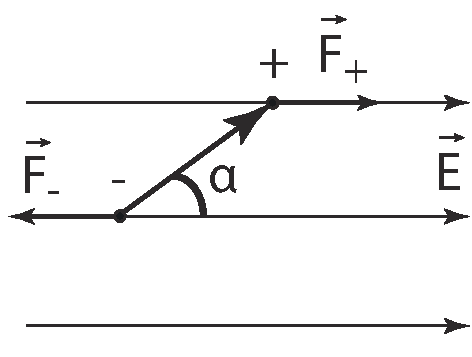
\includegraphics[width=.47\textwidth]{lec03/dipole_homogeneous.pdf}
        \hfill
        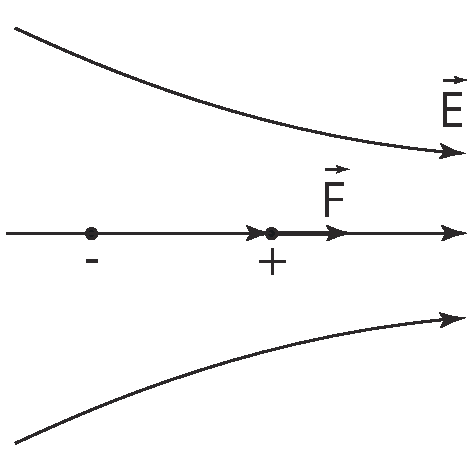
\includegraphics[width=.47\textwidth]{lec03/dipole_inhomogeneous.pdf}
        \parbox[t]{.47\textwidth}{\caption{Диполь в однородном поле}}
        \hfill
        \parbox[t]{.47\textwidth}{\caption{Диполь в неоднородном поле}}
    \end{figure}

    Пусть диполь помещён в однородное поле. Так как
    \( \vec{F_{-}} = -\vec{F_{+}} \), то \( \sum\vec{F} = 0 \). Однако, эта 
    пара сил создаёт момент \( M = lF_{+}\sin\alpha \) или
    \[
        \vec{M} = \vec{l}\times\vec{F_{+}} = q(\vec{l}\times\vec{E}) = 
        \vec{p}\times\vec{E}.
    \]
    
    Таким образом, в однородном поле действует момент:
    \begin{equation}
        \vec{M} = \vec{p}\times\vec{E}
    \end{equation}

    \subsection{Точечный диполь в неоднородном поле \textbf{E}}

    Момент сил, действующих на диполь, \( \vec{M} = \vec{p}\times\vec{E} \) 
    стремится повернуть диполь в ориентацию
    \( \vec{p} \uparrow\uparrow \vec{E} \). И если \( \vec{E} = \vec{E}(x,y,z)
    \ne \const \), то диполь втягивается в область более сильного поля.
    
    Вычислим энергию диполя в поле \( \vec{E} \).
    \( \sum\vec{F} = 0 \Rightarrow W_{\perp} = 0 \). Для поворота диполя в поле 
    \( \vec{E} \) необходимо совершить работу. Элементарная работа поворота:
    \[
        \dd A = M\dd\alpha = pE\sin\alpha \dd\alpha
    \]
    
    Тогда энергия диполя (ориентационная):
    \[
        W = A = \int pE\sin\alpha \dd\alpha = -pE\cos\alpha + C.
    \]
    Полагая, что при \( \vec{p} \perp \vec{E} \) энергия \( W = 0 \), получаем 
    \( C = 0 \). Таким образом,
    \begin{equation}
        W = -pE\cos\alpha = -\vec{p} \cdot \vec{E}.
    \end{equation}
    А так как в потенциальном поле \( \vec{F} = -\nabla W \), то в неоднородном 
    поле
    \[
        \vec{F} = \nabla(\vec{p}\cdot\vec{E}) = (\vec{p}\cdot\nabla)\vec{E}.
    \]
    
    В одномерном случае формула принимает вид
    \begin{equation}
        \vec{F}_x = p\frac{\partial E}{\partial x}
    \end{equation}

    \chapter{Проводник в электростатическом поле}

    \begin{definition}
        Проводник -- это твёрдое, жидкое или газообразное тело, у которого есть 
        свободные носители заряда (электроны или ионы), то есть заряды могут 
        свободно перемещаться по всему объёму тела.
    \end{definition}

    К проводникам относят: все металлы (в том числе и ртуть), их сплавы, 
    электролиты и ионизированный газ (плазма).

\section{Поле внутри сплошного проводника}

    \begin{proposition}
        Внутри сплошного проводника поле \( \vec{E} \) в любой точке равно нулю.
    \end{proposition}

    \( \vec{E}_{\textit{индуц}} = -\vec{E}_{\textit{внеш}} \). Если бы
    \( \vec{E}_{\textit{внутр}} \neq 0 \), то в проводнике был бы ток.

    \begin{remark}
        Однако, на создание индуцированных зарядов нужно время, но оно крайне
        мало: \( \tau_{\textit{релакс}} \sim 10^{-15} \text{ с} \).
    \end{remark}

    \begin{figure}[!b]
        \center
        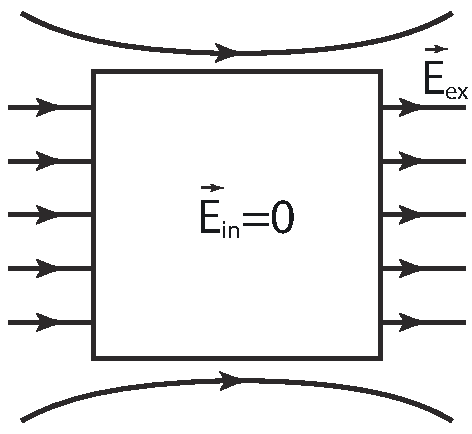
\includegraphics[width=0.47\textwidth]{lec04/solid_conductor.pdf}
        \hfill
        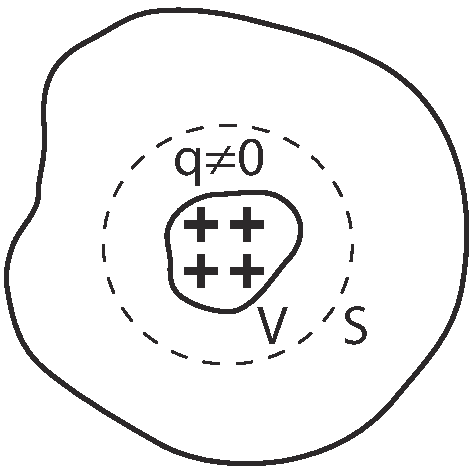
\includegraphics[width=0.47\textwidth]{lec04/solid_conductor_w-o_q.pdf}
        \parbox[t]{.47\textwidth}{
            \caption{Внутри проводника поля нет}
            \label{4:solid_conductor}
        }
        \hfill
        \parbox[t]{.47\textwidth}{
            \caption{Внутри проводника нет избыточного заряда}
            \label{4:conductor_w-o_q}
        }
    \end{figure}

    \begin{corollary}
        Вся область проводника -- эквипотенциаль.
    \end{corollary}
    \begin{proof}
         Так как \( \vec{E} = -\nabla\varphi \), то при
         \( \vec{E} \equiv 0,\ \varphi = \const \).
    \end{proof}


    \begin{corollary}
        Внутри сплошного проводника нет избыточного заряда.
    \end{corollary}
    \begin{proof}
        Допустим, что в некоторой области \( V \) внутри проводника
        \( q \ne 0 \). Эта ситуация представлена на
        рисунке~\ref{4:conductor_w-o_q}. Окружим эту область поверхностью
        \( S \). Тогда, так как \( \vec{E_{\textit{внутр}}} \equiv 0 \), то, по 
        теореме Гаусса:
        \[
            \oiint\limits_S \vec{E}\cdot\vec{dS} = \frac{q_S}{\varepsilon_0} 
            \Rightarrow q_S \equiv 0 \nonumber
        \]
    \end{proof}

\section{Поле у поверхности проводника}

    Докажем несколько утверждений:

    \begin{proposition}
        У поверхности проводника поле \( \vec{E} \) всегда перпендикулярно
        данному участку поверхности.
    \end{proposition}

    \begin{proof}
        Так как поверхность эквипотенциальна, то есть на ней
        \( \varphi = \const \), а \( \vec{E} = -\nabla\varphi \), а так как
        вектор \( \nabla\varphi \) всегда перпендикулярен поверхности уровня
        \( \varphi(x, y, z) \), то линии \( \vec{E} \) перпендикулярны
        поверхности проводника.
    \end{proof}
    \begin{comment}
        Если бы линии поля \( \vec{E} \) не были перпендикулярны поверхности 
        проводника, то \( \Delta\varphi = E\Delta l \), то есть поверхность
        была бы не эквипотенциальна, что противоречит утверждению.
    \end{comment}

    \begin{figure}[!b]
        \center
        \subfigure[Если бы поле было направлено таким образом,
                    то поверхность не была бы эквипотенциалью]{
            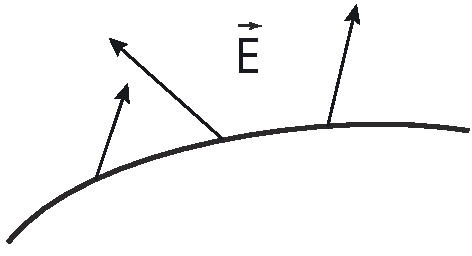
\includegraphics[width=0.3\textwidth]
                {lec04/perpendicular_field_wrong.pdf}
            \label{4:wrong}
        }
        \hfill
        \subfigure[Поле перпендикулярно поверхности проводника]{
            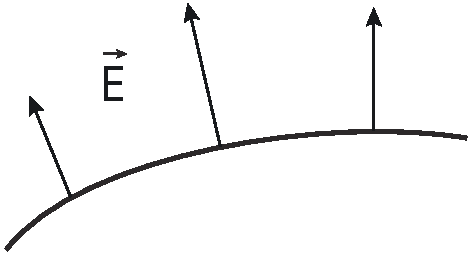
\includegraphics[width=0.3\textwidth]
                {lec04/perpendicular_field_right.pdf}
            \label{4:right}
        }
        \hfill
        \subfigure[К определению поля вблизи поверхности]{
            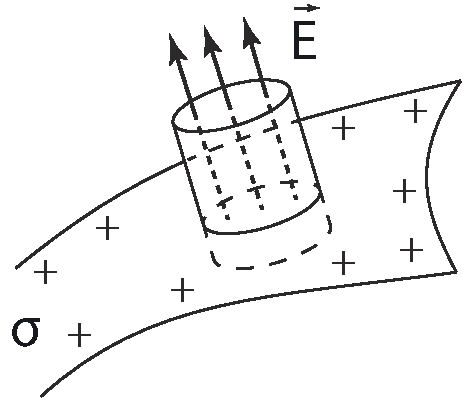
\includegraphics[width=0.3\textwidth]{lec04/conductor_surface.pdf}
            \label{4:conductor_surface}
        }
        \caption{Поле у поверхности проводника}
    \end{figure}

    \begin{proposition}
        У поверхности проводника
        \[
            \vec{E} = E_n = \frac{ \sigma }{ \varepsilon_0 },
        \]
        где \( \sigma \) -- поверхностная плотность заряда в данном месте 
        проводника.
    \end{proposition}

    \begin{proof}
        Охватим малый участок поверхности малым цилиндром. Тогда,
        по теореме Гаусса:
        \[
            \oiint\limits_S \vec{E}\cdot\vec{dS} = \frac{q_S}{\varepsilon_0} = 
            \frac{\sigma S_{\textit{тор}}}{\varepsilon_0}
        \]
        Но внутри проводника \( \vec{E} = 0 \), а вне него \( \vec{E} = E_n \), 
        следовательно
        \[
            \Phi_{S_{\textit{бок}}} = 0 \Rightarrow \oiint\limits_S \vec{E}
            \cdot \vec{dS} = ES_{\textit{тор}} \Rightarrow
            \vec{E}_{\textit{у поверхности}} = \frac{\sigma}{\varepsilon_0}.
        \]
    \end{proof}
    \begin{figure}[!b]
        \center
        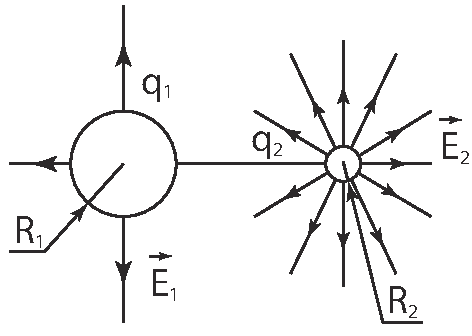
\includegraphics[width=0.47\textwidth]{lec04/E_and_R.pdf}
        \hfill
        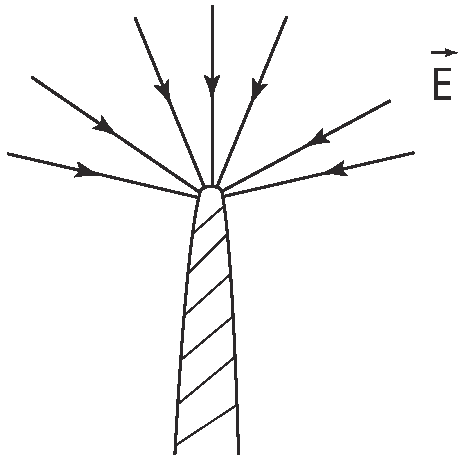
\includegraphics[width=0.47\textwidth]{lec04/needle.pdf}
        \parbox[t]{.47\textwidth}{
            \caption{Чем больше кривизна, тем сильнее поле}
            \label{4:E_and_R}
        }
        \hfill
        \parbox[t]{.47\textwidth}{
        \caption{Поле у острия иглы}
        \label{4:needle}
        }
    \end{figure}


    \begin{proposition}
        У поверхности проводника поле \( \vec{E} \) и плотность поверхностного
        заряда \( \sigma \) больше там, где больше кривизна участка поверхности
    \end{proposition}

    \begin{proof}
        Рассмотрим два металлических шара радиуса \( R_1 \) и \( R_2 \), 
        соединённых проволокой. Так как вблизи поверхности шара поле
        \[
            E = \frac{q}{4\pi\varepsilon_0 R^2},
        \]
        а потенциал металлического шара
        \[
            \varphi = \frac{q}{4\pi\varepsilon_0 R},
        \]
        то
        \[
            \varphi = ER \Rightarrow E_1 R_1 = E_2 R_2 \Rightarrow,
        \]
        и у поверхностей шаров
        \[
            \frac{E_2}{E_1} = \frac{R_1}{R_2},
        \]
        то есть
        \[
            E \sim \frac{1}{R}.
        \]
        А так как у поверхности проводника
        \[
            E = \frac{\sigma}{\varepsilon_0},
        \]
        то и
        \[
            \frac{\sigma_2}{\sigma_1} = \frac{R_1}{R_2}.
        \]
    \end{proof}

        \begin{comment}
        Пусть радиус острия иглы \( R = 10^{-6} \) м, тогда, при потенциале
        \( \varphi = 100 \) В, поле \( E \) у его поверхности
        \[
            E = \frac{\varphi}{R} = \frac{100}{10^{-6}} = 100 \cdot 10^6 =
            10^8 \frac{\text{В}}{\text{м}}.
        \]
    \end{comment}
    \begin{comment}
        При поле, большем чем \( E^{\text{возд}}_{\textit{проб}} =
        3 \cdot 10^6  (\text{В}/\text{м}) \) воздух будет пробит.
    \end{comment}

\section{Проводник с полостью в электрическом поле}
    \begin{figure}[b!]
        \center
        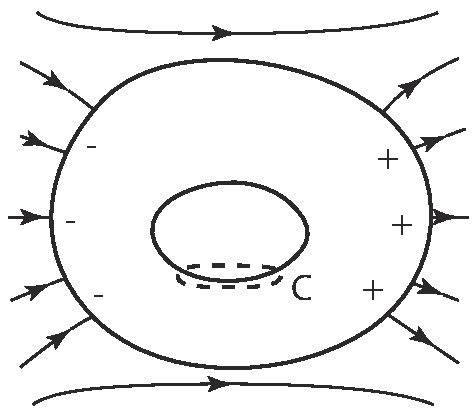
\includegraphics[width=0.47\textwidth]{lec04/holey_conductor.pdf}
        \hfill
        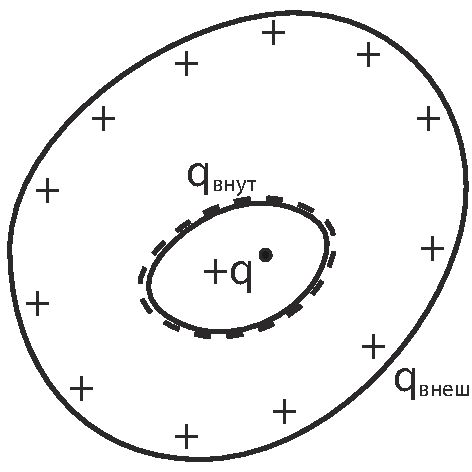
\includegraphics[width=0.47\textwidth]{lec04/q_in_ex.pdf}
        \parbox[t]{.47\textwidth}{\caption{Проводник с полостью}}
        \hfill
        \parbox[t]{.47\textwidth}{\caption{Проводник с зарядом в полости}}
    \end{figure}


    Поместим проводник с полостью во внешнее поле \( \vec{E} \). Тогда в
    полости:
    \begin{enumerate}
        \item \( \vec{E} \equiv 0 \);
        \item на внутренней поверхности полости \( \sigma \equiv 0 \).
    \end{enumerate}

    \begin{proof}
        Пусть \( \vec{E_{\textit{пол}}} \ne 0 \). А так как
        \( \vec{E_{\textit{пол}}} \) обязательно должно иметь источник, то
        \( \sigma_{\textit{пол}} \ne 0 \). % еще пикча

        Проведём контур \( C \) в полости по линии \( \vec{E} \),
        а в металле -- по любому пути. Тогда циркуляция:
        \[
            \oint\limits_C \vec{E}\cdot\vec{dl} = 
            \underbrace{\int\limits_{l_{\textit{пол}}} 
            \vec{E}_{\textit{пол}}\cdot\vec{dl}}_{\ne 0} + 
            \underbrace{\int\limits_{l_{\textit{мет}}} 
            \vec{E}_{\textit{мет}}\cdot\vec{dl}}_{= 0} \ne 0
        \]
        Но, по теореме о циркуляции поля \( \vec{E} \) следует, что
        \[
            \oint\limits_C \vec{E}\cdot\vec{dl} = 0.
        \]
        А так как \( \vec{E}_{\textit{мет}} = 0 \), то
        \( \vec{E}_{\textit{пол}} = 0 \). А так как
        \( \sigma = \varepsilon_0 E \), то и \( \sigma_{\textit{пол}} \).
    \end{proof}

 \section{Заряд в полости проводника}

    Пусть \( \vec{E}_{\textit{внеш}} = 0 \), а в полости находится заряд
    \( q \). Тогда:
    \begin{enumerate}
        \item \( q_{\textit{внутр}}^{\text{инд}} = -q \);
        \item \( q_{\textit{внеш}}^{\text{инд}} = +q \);
        \item Поле вне проводника \( \vec{E} \) создаётся только зарядом
            \( q_{\textit{внеш}}^{\text{инд}} \) на внешней поверхности и от 
            положения \( q \) в полости не зависит.
    \end{enumerate}

    \begin{proof}
    \begin{enumerate}
        \item Охватим полость замкнутой поверхностью \( S \) по металлу.
            Так как на ней \( \vec{E}_{\textit{мет}} \equiv 0 \), то:
            \[
                \oiint\limits_S \vec{E}_{\textit{мет}}\cdot\vec{dS} = 
                \frac{q_S}{\varepsilon_0} = 0 \Rightarrow q_S = q + 
                q_{\textit{внутр}}^{\text{инд}} = 0 \Rightarrow 
                q_{\textit{внутр}}^{\text{инд}} = -q
            \]
        \item Так как образец в целом нейтрален, то
            \[
                q_{\textit{внеш}}^{\text{инд}} =
                -q_{\textit{внутр}}^{\text{инд}} = +q
            \]
        \item Так как в металле \( \vec{E}_{\textit{мет}} \equiv 0 \), то  можно 
            удалить полость с зарядом \( q \) на бесконечность или залить её 
            металлом. Внешнее поле \( \vec{E} \) от этого не изменится.
    \end{enumerate}
    \end{proof}

    Таким образом, \textbf{металлическая оболочка разделяет всё пространство
    на две электронезависимых области: внутри и снаружи. Всякие изменения
    внутри не влияют на поле снаружи, и наоборот}.

    Частным вариантом оболочки является бесконечная металлическая плоскость, 
    разделяющая всё пространство на два электронезависимых полупространства.

\section{Основная задача электростатики}

    \begin{figure}[t!]
        \center
        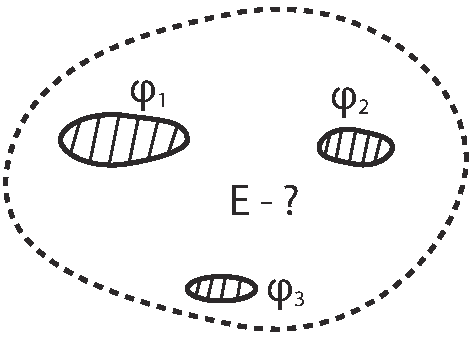
\includegraphics[width=0.5\textwidth]{lec04/E_from_phi.pdf}
        \caption{Основная задача электростатики}
    \end{figure}

    Если в пространстве известно распределение потенциала
    \( \varphi(x, y, z) \), то поле \( \vec{E} \) легко вычисляется:
    \( \vec{E} = -\nabla\varphi \).

    Основная задача электростатики формулируется так: пусть заданы геометрии
    всех проводников и диэлектриков, заданы либо заряды на них, либо их
    потенциалы. Определить поле \( \varphi(x, y, z) \) во всём пространстве.

    \begin{solution}
        Из теоремы Гаусса:
        \[
            \left\{
            \begin{array}{l}
                \div{\vec{E}} = \frac{\rho(x, y, z)}{\varepsilon_0}, \\
                \vec{E} = -\nabla\varphi.
            \end{array} \right.
        \]
        Тогда
        \[
            \div\grad\varphi = -\frac{\rho(x, y, z)}{\varepsilon_0}.
        \]

        Таким образом,
        \begin{equation}
            \label{eq4:1}
            \Delta\varphi = -\frac{\rho}{\varepsilon_0},
        \end{equation}
        Где \( \Delta \) -- оператор Лапласа.
    \end{solution}

    Уравнение (\ref{eq4:1}) называется \textit{уравнением Пуассона}. Обычно, в
    воздухе или  в вакууме, \( \rho(x, y, z) = 0 \). И тогда уравнение Пуассона
    преобразуется в уравнение Лапласа:
    \begin{equation}
        \label{eq4:2}
        \Delta\varphi = 0
    \end{equation}

    В теории дифференциальных уравнений доказывается теорема о единственности:

    \begin{theorem}
        Дифференциальное уравнение (\ref{eq4:2}) в частных производных с
        заданными граничными условиями (потенциалом или напряжённостью на
        границе области) имеет единственное решение.
    \end{theorem}

    В общем случае эта задача аналитического решения не имеет, однако, для
    некоторых симметричных зарядовых систем это решение есть. Одним из методов
    решения (\ref{eq4:2}) аналитически является \textit{метод изображений}.

\section{Метод изображений}

    \begin{figure}[t!]
        \center
        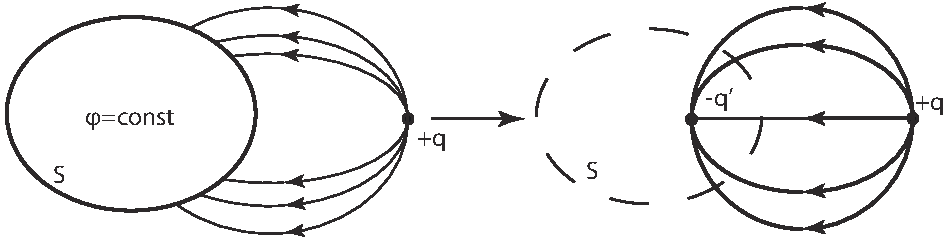
\includegraphics[width=0.7\textwidth]{lec04/images_method.pdf}
        \caption{Метод иображений}
    \end{figure}

    \begin{definition}
        \textbf{Метод изображений} -- это специальный приём расчёта
        электрического поля систем ``заряд -- металлическая поверхность''.
    \end{definition}

    Пусть задана металлическая поверхность \( S \) и заряд \( q \) вблизи неё.
    Найти либо поле \( \vec{E} \), либо потенциал \( \varphi(x, y, z) \). Тогда
    решение этой задачи методом изображений будет таково:

    Если удастся построить такую систему заряда или зарядовой конфигурации,
    которая бы вместе с исходным зарядом \( q \) создавала систему
    эквипотенциальных поверхностей, одна из которых совпадает с исходной
    поверхностью \( S \), то металлическое тело можно удалить, и при этом поле
    вне поверхности \( S \) не изменится.

    Таким образом, задача ``заряд -- металлическая поверхность'' в точности
    совпадает с задачей ``заряд -- группа зарядов''. Эта группа зарядов
    \( q_i \) называется \textit{изображением} заряда \( q \)  в поверхности
    \( S \).

    Рассмотрим работу метода изображений на примере системы ``заряд --
    металлическая плоскость'':
    \begin{figure}[b!]
        \center
        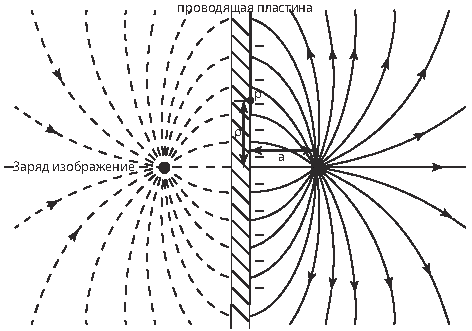
\includegraphics[width=0.7\textwidth]{lec04/flat_image.pdf}
        \caption{Применение метода изображений к системе ``заряд -- 
            металлическая плоскость''}
    \end{figure}
    \begin{example}
        На высоте \( h \) над бесконечной металлической плоскостью находится
        точечный заряд \( q \). Определить поле \( \vec{E} \) во всем верхнем
        полупространстве.
    \end{example}

    \begin{solution}
        Здесь очевидно, что эта бесконечная плоскость является эквипотенциалью 
        системы “\( +q \) -- \( -q \)”, где \( -q \) -- изображение заряда
        \( +q \) на металлическую плоскость, то есть если заменим бесконечную 
        плоскость зарядом \( -q \) на расстоянии \( h \) под плоскостью, то
        поле \( \vec{E} \) при \( z > 0 \) не изменится.

        А поле системы \( \{ q^{+}, q^{-} \} \) -- легко считается. Тогда вблизи 
        плоскости (при \( z \approx 0 \)) поле пары зарядов:
        \[
            E_{+} = \frac{q}{4\pi\varepsilon_0 {r'}^2}
        \]
        r -- расстояние от точки \( M \) до точки \( O \).Тогда результирующее
        поле:
        \[
            E_{\textit{рез}} = 2E_{+}\sin\alpha = 2E_{+}\frac{h}{r'} = 
            \frac{2qh}{4\pi\varepsilon_0(r^2 + h^2)^{\frac{3}{2}}}
        \]
        А так как \( \sigma = \varepsilon_0 E \), то распределение
        индуцированных зарядов на плоскости:
        \[
            \sigma(r) = -\frac{qh}{2\pi(r^2+h^2)^{\frac{3}{2}}}
        \]
    \end{solution}

    \begin{remark}
        Если вместо точечного заряда \( q \) над плоскостью натянут провод с 
        погонной плотностью заряда \( \gamma (\text{Кл}/\text{м})\), то
        его изображением в плоскости будет провод \( -\gamma \), а поле системы 
        ``провод -- земля'' тождественно равно полю системы ``проводник --
        проводник''.
        \[
            E_{+} = \frac{\gamma}{2\pi\varepsilon_0 r'} \nonumber
        \]
        Тогда результирующее поле:
        \[
            E = 2E_{+}\sin\alpha = 2\frac{\gamma}{2\pi\varepsilon_0 r}
            \frac{h}{r'} = \frac{\gamma h}{\pi\varepsilon_0 {r'}^2} =
            \frac{\gamma h}{\pi\varepsilon_0(r^2 + h^2)}
        \]
    \end{remark}

\section{Ёмкость уединённого проводника}

    Рассмотрим уединённый проводник. Поместим на него заряд \( q \), он 
    распределится по поверхности проводника, следовательно, появится
    электрическое поле \( \vec{E} \) и потенциал \( \varphi \) образца станет
    не равен нулю.
    \[
        \varphi = \int\limits_{\textit{поверхность}}^{\infty}
        \vec{E}\cdot\vec{dl}
    \]

    Опыт показывает, что потенциал \( \varphi \sim q \). Следовательно,
    \begin{equation}
        \label{eq4:C1}
        q = C\varphi
    \end{equation}

    \begin{definition}
        Коэффициент пропорциональности  \( C \) между зарядом проводника и его 
        потенциалом в (\ref{eq4:C1}) называется \textbf{электроёмкостью}
        проводника.
    \end{definition}

    Таким образом, по определению:
    \[
        C = \frac{q}{\varphi}
    \]

    Ёмкость измеряется в фарадах:
    \[
        C = 1\text{ Ф} = \frac{q = 1 \text{ Кл}}{\varphi = 1 \text{ В}}
    \]

    \begin{example}
        Определить радиус металлического шара с ёмкостью \( C = 1\) Ф.
    \end{example}

    \begin{solution}
        Решим эту задачу пошагово:
        \begin{enumerate}
            \item Поместим на шар заряд \( q \).
            \item Вычислим потенциал шара:
                \[
                    \varphi = \frac{q}{4\pi\varepsilon_0 R}.
                \]
            \item По определению:
                \[
                    C = \frac{q}{\varphi} = 4\pi\varepsilon_0 R.
                \]
            \item
                \[
                    R = \frac{C}{4\pi\varepsilon_0} =
                    \frac{1}{4\pi\varepsilon_0} \approx 10^10 \text{ м} =
                    10^7 \text{ км}.
                \]
        \end{enumerate}
        \end{solution}

\section{Конденсатор}
    \begin{figure}[b!]
    \center
    \subfigure[Конденсатор]{
        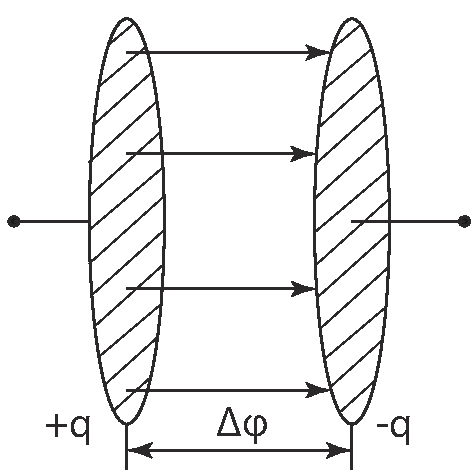
\includegraphics[width=0.3\textwidth]{lec04/capacitor.pdf}
    }
    \hfill
    \subfigure[Плоский конденсатор]{
        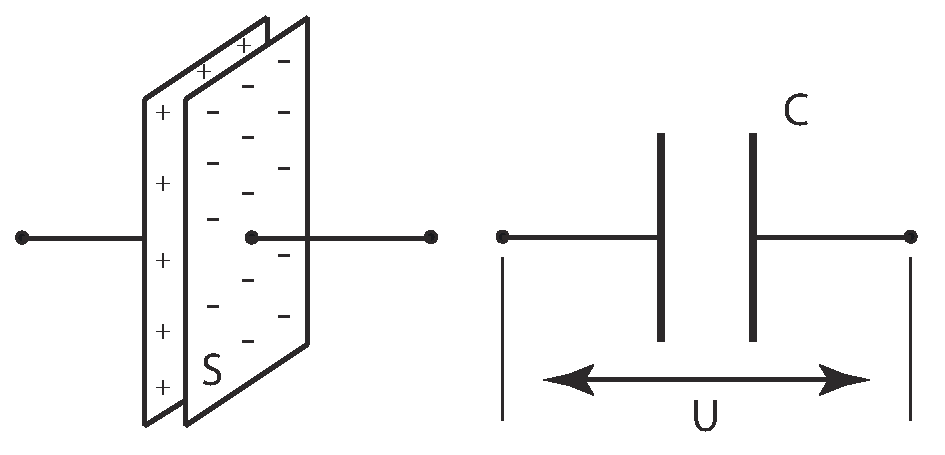
\includegraphics[width=0.6\textwidth]{lec04/flat_capacitor.pdf}
    }
    \caption{Конденсаторы}
    \end{figure}


    Если к уединённому заряженному проводнику приблизить другой, то полученная 
    система может быть использована для накопления электрического заряда.

    \begin{definition}
        Система двух близко расположенных проводников называется
        \textbf{конденсатором}.
    \end{definition}

    Выражение ``зарядить конденсатор'' означает внесение на его обкладки равные
    заряды \( +q \) и \( -q \), где \( q = +q = |-q| \) -- называется зарядом
    конденсатора. Опыт показывает, что \( \Delta\varphi \sim q \), или:
    \begin{equation}
        \label{eq4:C2}
        q = C \Delta\varphi
    \end{equation}

    \begin{definition}
        Коэффициент пропорциональности \( C \) между зарядом конденсатора и его
        разностью потенциалов на его обкладках в (\ref{eq4:C2}) называется
        \textbf{ёмкостью} конденсатора. Таким образом, по определению,
        \[
            C \equiv \frac{q}{\Delta\varphi}.
        \]
    \end{definition}

    \begin{remark}
        Разность потенциалов \( \Delta\varphi \) называется \textbf{напряжением}
        на конденсаторе \( U = \Delta\varphi \). Таким образом,
        \[
            C = \frac{q}{U}.
        \]
    \end{remark}

    Так как фарад величина очень большая (\textit{ёмкостью 1 Ф обладал бы 
    уединённый шар, радиус которого больше, чем 10 радиусов Солнца}), то на 
    практике используют производные величины от фарада: \( 1\text{ мкФ} =
    1 \cdot 10^{-6}\text{ Ф} \), \( 1\text{ нФ} = 1 \cdot 10^{-9}\text{ Ф} \),
    \( 1\text{ пФ} = 1 \cdot 10^{-12}\text{ Ф} \).

        \begin{definition}
        Конденсатор называется \textbf{плоским}, если его обкладками являются
        пара близких параллельных плоскостей. % пикча
    \end{definition}

    Вычислим ёмкость плоского конденсатора (\( S, d \)). % пикча 1 & 2
    \begin{enumerate}
        \item Зарядим конденсатор.
        \item Вычислим поле \( \vec{E} \) между обкладками.
        Так как каждая заряженная плоскость создаёт вокруг себя поле
        \[
            E = \frac{\sigma}{2\varepsilon_0},
        \]
        то их суммарное поле равно
        \[
            E = \frac{\sigma}{\varepsilon_0}.
        \]
         Это и есть поле в конденсаторе:
         \[
             E = \frac{\sigma}{\varepsilon_0} = \frac{q}{\varepsilon_0 S}.
         \]
        \item Вычислим напряжение:
            \[
                U = \Delta\varphi = Ed = \frac{qd}{\varepsilon_0 S}.
            \]
        \item По определению:
        \[
            C = \frac{q}{U} = \frac{q\varepsilon_0 S}{qd} =
            \frac{\varepsilon_0 S}{d}.
        \]
    \end{enumerate}

    \begin{example}
        Вычислить ёмкость плоского конденсатора, площадь обкладок которого
        \( S = 1 \text{м}^2\) и расстояние между ними \( d = 10^{-6} \) м.
    \end{example}

    \begin{solution}
        \[
            C = \frac{\varepsilon_0 S}{d} = \frac{10^{-11} \cdot 1}{10^{-6}} =
            10^{-5} \text{ Ф} = 10 \text{ мкФ}
        \]
    \end{solution}

    \begin{example}
        Вычислить погонную ёмкость цилиндрического конденсатора (коаксиальной
        линии), если радиусы цилиндров \( R_2 \) и \( R_1 \) такие, что 
        \( R_2 > R_1 \), а длина цилиндров \( l \gg R_2 \).
    \end{example}

    \begin{figure}[t!]
        \center
        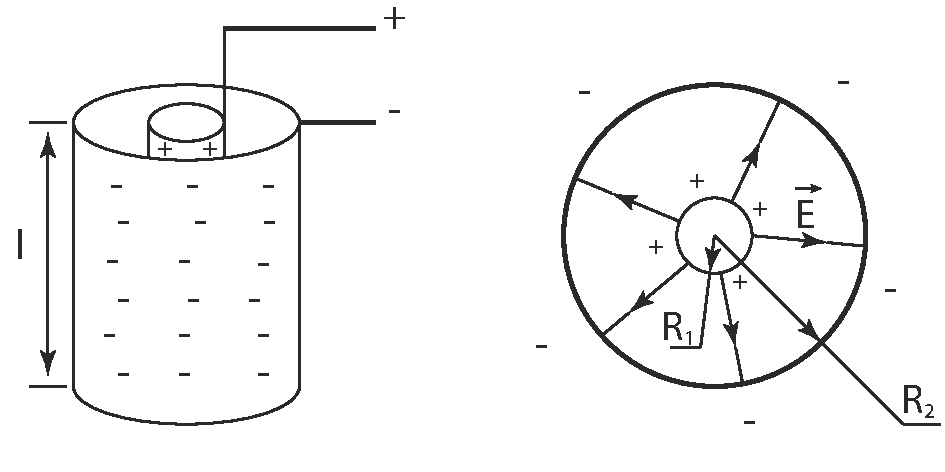
\includegraphics[width=0.6\textwidth]{lec04/cylinder_capacitor.pdf}
        \caption{Цилиндрический конденсатор}
    \end{figure}

    \begin{solution}
        \begin{enumerate}
            \item Заряжаем конденсатор до заряда \( q = \gamma l \).
            \item Поле между цилиндрами, то есть \( R_1 < r < R_2 \):
            \[
                 E = \frac{\gamma}{2\pi\varepsilon_0 r}.
            \]
            \item Напряжение:
            \[
                U = \Delta\varphi = \int\limits_{R_1}^{R_2} Edr = 
                \int\limits_{R_1}^{R_2} \frac{\gamma}{2\pi\varepsilon_0 r}dr = 
                \frac{\gamma}{2\pi\varepsilon_0}\ln\frac{R_2}{R_1} = 
                \frac{q}{2l\pi\varepsilon_0}\ln\frac{R_2}{R_1}.
            \]
            \item Ёмкость:
            \[
                C = \frac{q}{U} =
                \frac{q \cdot 2l\pi\varepsilon_0 } {q\ln\frac{R_2}{R_1}} = 
                \frac{2\pi\varepsilon_0 l}{\ln\frac{R_2}{R_1}}.
            \]
            \item Погонная ёмкость коаксиальной линии:
            \[
                C_0 = \frac{C}{l} = \frac{2\pi\varepsilon_0}{\ln\frac{R_2}{R_1}} 
                \left(\frac{\text{Ф}}{\text{м}}\right).
            \]
        \end{enumerate}
    \end{solution}

\section{Соединение конденсаторов}

    \begin{figure}[b!]
        \center
        \subfigure[Параллельно]{
            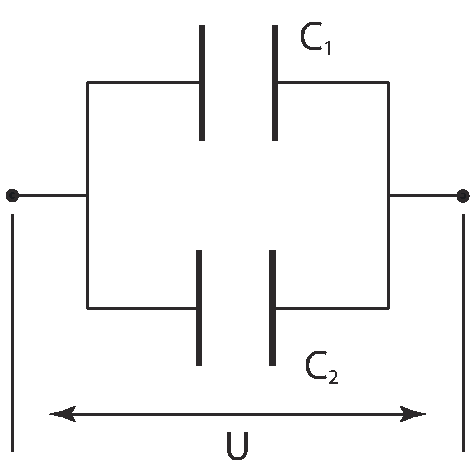
\includegraphics[width=0.47\textwidth]{lec04/C_parallel.pdf}
        }
        \hfill
        \subfigure[Последовательно]{
            \includegraphics[width=0.47\textwidth]{lec04/C_serial.pdf}
        }
        \caption{Соединения конденсаторов}
    \end{figure}
    \begin{enumerate}
        \item Параллельное:
        \begin{align}
        \left\{
        \begin{array}{rl}
            q_{ab} = & q_1 + q_2 \\
            U_{ab} = & U_1 = U_2
        \end{array} \right. \nonumber \\
        C_{ab} = C_1 + C_2 \nonumber
        \end{align}
        \item Последовательное: % пикча
        \begin{align}
        \left\{
        \begin{array}{rl}
            U_{ab} = & U_1 + U_2 \\
            q_{ab} = & q_1 = q_2
        \end{array} \right. \nonumber \\
        \frac{1}{C_{ab}} = \frac{1}{C_1} + \frac{1}{C_2} \nonumber
        \end{align}
    \end{enumerate}

\section{Энергия заряженного конденсатора}

    %пикча
    Pарядка конденсатора -- это процесс разделение зарядов, для проведения
    которого необходимо совершать работу против поля \( \vec{E} \).

    Пусть \( q' \) -- текущий заряд на обкладках, \( \vec{E}' \) -- текущее
    поле в процессе зарядки, \( U' \) -- текущее напряжение, \( dq' \) --
    очередная порция переносимого заряда каким-либо внешним устройством 
    (генератором).

    Тогда элементарная работа внешних сил по переносу очередной порции заряда
    \( dq' \) с левой обкладки на правую, с более высоким потенциалом, по 
    определению может быть вычислена как \( dA = U' dq' \), а поскольку
    \( U' = \frac{q'}{C} \), то энергия заряженного конденсатора до его полной 
    зарядки, то есть до скопления зарядов \( q \) и \(-q \) на обкладках:
    \[
        W = A = \int\limits_0^q \frac{q' dq'}{C} = \frac{q^2}{2C}
    \]
    А так как \( q = CU \), то:
    \begin{equation}
        \label{eq4:C3}
        W = \frac{CU^2}{2}
    \end{equation}

    \begin{figure}[b!]
        \center
        \includegraphics[width=0.47\textwidth]{lec04/flat_capacitor_field.pdf}
        \caption{Поле плоского конденсатора}
    \end{figure}

\section{Локализация энергии в электростатическом поле}

    % пикча
    Рассмотрим плоский конденсатор \( C \):
    \[
        C = \frac{\varepsilon_0 S}{d}.
    \]
    Энергия \( W \), накопленная в нем:
    \[
        W = \frac{CU^2}{2}.
    \]
    Эта энергия локализована в электрическом поле между обкладками конденсатора.
    Вычислим её плотность
    \[
        w = \frac{W}{V} \, \left(\frac{\text{Дж}}{\text{м}^3}\right).
    \]

    Так как \( U = Ed\) и \( C = \frac{\varepsilon_0 S}{d} \), то:
    \[
        W = \frac{\varepsilon_0 S}{2d} \cdot E^2 d^2 =
        \frac{\varepsilon_0 S E^2 d}{2} = [ S \cdot d = V_E ] =
        \frac{\varepsilon_0 E^2}{2} V_E,
    \]
    где \( V_E \) -- объем, занимаемый электрическим полем. В случае плоского 
    конденсатора \( V_E = V \).

    Тогда,
    \[
        w = \frac{\varepsilon_0 E^2}{2}.
    \]

    \chapter{Электрическое поле в диэлектриках}

\section{Поляризация диэлектриков}

    \begin{definition}
        \textbf{Диэлектрики} -- это вещества, которые не имеют свободных
        зарядов, то есть таких зарядов, которые могли бы перемещаться по всему
        объёму тела. Заряды в них могут смещаться лишь на расстояния порядка
        межатомных.
    \end{definition}
    
    Однако, при помещении диэлектрика в электрическое поле он начинает
    взаимодействовать с ним:
    
    \begin{enumerate}
        \item заметно искажение поле;
        \item диэлектрик приобретает заметный макроскопический момент, из-за
            которого он начинает взаимодействовать с полем: ориентируется и
            втягивается в область более сильного поля
            \[
                F = p\frac{\partial E}{\partial x}; \ p = ql \ne 0
            \]        
    \end{enumerate}
    
    \begin{definition}
    Разделение зарядов в диэлектрике и появление у него дипольного момента при
    помещении во внешнее электрическое поле \( \vec{E} \) называется
    \textbf{поляризацией} диэлектрика во внешнем электрическом поле
    \( \vec{E} \).
    \end{definition}
    
    В зависимости от структуры и химического состава возможны несколько
    механизмов поляризации диэлектрика.
    
\section{Механизмы поляризации}

\subsection{Электронная поляризация}
    По этому механизму поляризуются диэлектрики, молекулы которых не имеют
    собственного дипольного момента (\( p_i = 0 \)), например,
    \( H_2, O_2, CH_4, CO_2 \).
    
    Однако, при их помещении в поле \( \vec{E} \) электронная оболочка слегка
    деформируется и каждая молекула приобретает дипольный момент, и,
    следовательно, весь диэлектрик приобретает дипольный момент.
    
\subsection{Ориентационная поляризация}

    Этот механизм наблюдается у веществ, молекулы которых имеют собственный
    дипольный момент (\( p_i \ne 0 \)), таких как \( H_2O \text{ и } NH_3\).
    В отсутствие внешнего поля, все эти элементарные диполи ориентированы
    хаотично, и образец в целом нейтрален. Но при наложении поля элементарные
    диполи \textit{слегка} выстраиваются вдоль линий поля.
    
\subsection{Ионная поляризация}

    Этот механизм наблюдается у ионных кристаллов. Рассмотрим его на примере
    \( Na^{+}Cl^{-} \). В отсутствие внешнего поля решётки \( Na^{+} \) и
    \( Cl^{-} \) располагаются так, что кристалл нейтрален. При наложении поля,
    решётки \textit{немного} смещаются и, в результате, кристалл поляризуется.
    
\subsection{Механическая поляризация (пьезоэлектрический эффект)}

    Механизм наблюдается у кристаллов, не имеющих центра симметрии, например,
    \( BaTiO_3 \). При этом меанизме поляризации кристалл поляризуется под
    воздействием внешних механических напряжений.
      
\section{Поверхностные и объёмные связанные заряды}

    При поляризации однородного диэлектрика поляризационные, или
    \textbf{связанные}, заряды выделяются только на его поверхности.
    Однако, разделить их нельзя, так как получится два поляризованных образца.
    Если же диэлектрик неоднороден, то при помещении его во внешнее поле
    \( \vec{E} \), в нем появляются не только поверхностные, но и объёмные
    связанные заряды.
    \begin{figure}[b!]
        \center
        \subfigure[Однородный диэлектрик]{
            \includegraphics[width=0.47\textwidth]{lec05/homogeneous.pdf}
        }
        \hfill
        \subfigure[Неоднородный диэлектрик]{
            \includegraphics[width=0.47\textwidth]{lec05/inhomogeneous.pdf}
        }
        \caption{Связанные заряды в диэлектриках}
    \end{figure}
\section{Поляризованность}
    
    Количественной характеристикой степени поляризации диэлектрика является его
    \textbf{поляризованность}.
    
    \begin{definition}
        \textbf{Поляризованность} \( \vec{P} \) -- это дипольный момент единицы
        объёма диэлектрика.
    \end{definition}
    \begin{equation}
        \vec{P} = \frac{\sum \vec{p_i}}{\Delta V} = n \midnum{\vec{p_i}},
    \end{equation}
    где \( \vec{P} \) -- вектор поляризованности, \( \vec{p_i} \) -- дипольный
    момент \( i \)-молекулы,
    \( \midnum{\vec{p_i}} = \frac{\sum \vec{p_i}}{N} \) -- средний дипольный
    момент одной молекулы, \( n = \frac{N}{\Delta V} \) -- концентрация молекул,
    \( N \) -- количество молекул в единице объёма.
    
    Если поляризация \textbf{однородная}, то есть однороден поляризованный
    диэлектрик, то поверхностную плотность \( \sigma' \) связанного
    поверхностного заряда можно легко связать с вектором поляризованности
    \( \vec{P} \). Для этого вырежем из диэлектрика косую призму и определим её
    дипольный момент:
    \[
        p = q' l = \sigma' Sl
    \]
    Объем призмы:
    \[
        V = lS_{\perp} = lS\cos\alpha
    \]
    
    Тогда, по определению:
    \[
        P = \frac{p}{V} = \frac{\sigma'}{\cos\alpha}
    \]
    Или:
    \begin{equation}
        \sigma' = P\cos\alpha = P_n,
    \end{equation}
    где \( P_n \) -- нормальная компонента вектора \( \vec{P} \).
    
    Если поляризация неоднородная, то, в общем случае, для него справедлива
    теорема Гаусса для поля вектора \( \vec{P} \):
    \begin{theorem}
        Поток вектора \( \vec{P} \) через произвольную замкнутую поверхность
        \( S \) равен суммарному связанному заряду \( q_S' \), охваченному
        поверхностью \( S \).
        \begin{equation}
            \oiint\limits_S \vec{P}\cdot\vec{dS} = -q_S' \label{eq5:X3n1}
        \end{equation}
    \end{theorem}
    
    
    Если заряд \( q' \) распределён по образцу непрерывно, то
    \[
        q_S' = \iiint\limits_V \rho' dV.
    \]
    А так как по теореме Остроградского
    \[
        \oiint\limits_S \vec{P}\cdot\vec{dS} = \iiint\limits_V \div\vec{P}dV,
    \]
    то, в силу произвольности \( S \) и \( V \):
    \begin{equation}
        \rho' = -\div\vec{P} \label{eq5:X3n2}
    \end{equation}
    Уравнение (\ref{eq5:X3n2}) -- это дифференциальная форма теоремы Гаусса для
    вектора \( \vec{P} \).
    
\section{Электрическое поле в диэлектриках}
    
    \begin{figure}[b!]
        \center
        \includegraphics[width=0.47\textwidth]{lec05/E_and_isolator.pdf}
        \caption{Электрическое поле в диэлектриках}
    \end{figure}

    Появление индуцированных связанных зарядов в образце при его помещении во
    внешнее поле \( \vec{E_0} \) порождает индуцированное поле \( \vec{E'} \),
    которое, складываясь с \( \vec{E_0} \), и даёт результирующее внешнее поле
    \( \vec{E} \):
    \begin{equation}
        \vec{E} = \vec{E_0} + \vec{E'}
    \end{equation}
    % еще есть много надписей, видимо относящихся к картинке:
    %  \( \Delta\varphi = 0 \) или \( \Delta\varphi = -\frac{\rho}{\eps_0} \) для нахождения результирующего поля \( \vec{E} \), так как заряды создают поле \( \vec{E} \) и конфигурируются им.

\section{Вектор \textbf{D}}

    Так как поле \( \vec{E} \) создаётся всеми зарядами: и свободными \( q \),
    и связанными \( q' \), то теорема Гаусса для поля \( \vec{E} \) будет
    выглядеть так:
    \begin{equation}
        \oiint\limits_S \vec{E}\cdot\vec{dS} = \frac{1}{\eps_0}(q+q')_S
        \label{eq5:1}
    \end{equation}
    
    Чтобы избавиться от неизмеряемого заряда \( q_S' \) применим теорему Гаусса для поля \( \vec{P} \) и тогда (\ref{eq5:1}):
    \[
        \oiint\limits_S (\eps_0\vec{E} + \vec{P})\cdot\vec{dS} = q_S
    \]
    
    Обозначим комбинацию в скобках за \( \vec{D} \):
    \begin{equation}
        \vec{D} = \eps_0\vec{E} + \vec{P} \label{eq5:2}
    \end{equation}
    
    Тогда теорема Гаусса для поля \( \vec{D} \):
    \begin{equation}
        \oiint\limits_S \vec{D}\cdot\vec{\dd S} = q_S
        \label{eq5:3}
    \end{equation}
    
    При непрерывном распределении заряда
    \[
        q_S = \iiint\limits_V \rho \dd V.
    \]
    Тогда, по теореме Остроградского:
    \[
        \oiint\limits_S \vec{D}\cdot\vec{dS} = \iiint\limits_V \div\vec{D}\dd V 
    \]
    
    В силу произвольности \( S \) и \( V \):
    \begin{equation}
        \div\vec{D} = \rho \label{eq5:4}
    \end{equation}
    
    Уравнение (\ref{eq5:4}) -- дифференциальная форма теоремы Гаусса для поля
    \( \vec{D} \). Таким образом, источником поля \( \vec{D} \) являются только
    свободные (избыточные), заряды, а поля \( \vec{E} \) -- и избыточные,
    и связанные.
     
\section{Связь между векторами \textbf{P}, \textbf{E} и \textbf{D}}

    Так как обычные (\( E \ll E_{\textit{межатом}} \sim
    10^{11} \text{В}/\text{м} \)) поля вызывают слабую деформацию
    электронных оболочек, то можно считать, что \( P \sim E \), а так как по
    размерности \( [P] = [\eps_0E] \) и
    \( \vec{P} \uparrow\uparrow \vec{E} \) в изотропных диэлектриках, то можно
    считать, что
    \begin{equation}
        \vec{P} = \varkappa\eps_0\vec{E} \label{eq5:5}
    \end{equation}
    
    Безразмерный множитель \( \varkappa \) в (\ref{eq5:5}) называетс
    \textbf{диэлектрической восприимчивостью} диэлектрика.
    
    Подставив (\ref{eq5:5}) в (\ref{eq5:2}), получаем:
    \begin{equation}
        \vec{D} = \eps_0\vec{E}(\varkappa+1) =
        \eps\eps_0\vec{E}
        \label{eq5:6}
    \end{equation}
    
    Скалярный множитель \( \eps \) называется
    \textbf{диэлектрической проницаемостью} вещества. Обычно, для диэлектриков
    \( \eps \sim 1\ldots3\):
    \begin{itemize}
        \item для вакуума: \( \eps = 1 \),
        \item для воздуха: \( \eps = 1.0006 \),
        \item для стекла: \( \eps \sim 1.5 \),
        \item но для воды: \( \eps = 81 \).
    \end{itemize}
    
    Формулы (\ref{eq5:2}), (\ref{eq5:5}) и (\ref{eq5:6}) выражают искомую связь
    между векторами \( \vec{P}, \vec{E} \) и \( \vec{D} \).
    
\section{Конденсатор с диэлектриком}

    Ёмкость конденсатора с диэлектриком будет увеличена, так как связанные
    заряды уменьшают поле \( \vec{E} \), следовательно, уменьшается  напряжение
    \( U \), следовательно увеличивается \( C \), так как
    \( C\uparrow = \frac{q=\const}{U\downarrow} \).
    \begin{figure}[h]
        \center
        \includegraphics[width=0.47\textwidth]{lec05/capacitor.pdf}
        \caption{Конденсатор с диэлектриком}
    \end{figure}
    Вычислим ёмкость конденсатора, заполненного диэлектриком с диэлектрической
    проницаемостью \( \eps \). Для пустого плоского конденсатора
    \[
        C_0 = \frac{\eps_0S}{d}.
    \]
    Пусть в нем находится диэлектрик \( \eps \). Охватим участок верхней
    пластины замкнутым цилиндром
    \( S_{\textit{цил}} = S_{\textit{бок}} + 2S_{\textit{тор}} \).
    
    Так как вне конденсатора \( E = 0 \) и \( D = 0 \), то, по теореме Гаусса:
    \[
        \underbrace{\oiint\limits_{ S_{\textit{цил}} }\vec{D}\cdot\vec{dS}
        }_{DS_{\textit{тор}}} = q_S = \sigma S_{\textit{тор}}
    \]
    
    Тогда \( \sigma = D \), где \( \sigma \) -- поверхностная плотность
    свободных зарядов. И тогда
    \[
        C = \frac{q}{U} = \frac{\sigma S}{Ed} = \frac{DS}{Ed} =
        \frac{\eps\eps_0 S}{d} = \eps C_0
    \]
    
    Таким образом, ёмкость конденсатора с диэлектриком в \( \eps \) раз
    больше, чем ёмкость пустого конденсатора.
    
\section{Распределение энергии в электрическом поле}

    Запишем энергию плоского конденсатора с диэлектриком:
    \[
        W = \frac{CU^2}{2} = \frac{\eps\eps_0E^2Sd}{2} =
        \frac{\eps\eps_0E^2}{2}V_E,
    \]
    где \( V_E \) -- объем, занимаемый полем \( \vec{E} \). Таким образом,
    \( W \sim V_E \). Можно предположить, что энергия локализована в поле
    \( \vec{E} \).
    
    Тогда объёмная плотность энергии электрического поля:
    \[
        w_E = \frac{W}{V_E} = \frac{\eps\eps_0E^2}{2} =
        \frac{ED}{2} \left(\frac{\text{Дж}}{\text{м}^3}\right)
    \]
    
\section{Граничные условия}

    Пусть два диэлектрика \( \eps_1 \) и \( \eps_2 \) с общей
    границей их раздела помещены во внешнее поле \( \vec{E_0} \). Линии поля
    \( \vec{E_0} \) на границе раздела будут испытывать преломление, так как
    на границе появятся заряды \( \pm \sigma' \).
    
    Установим характер преломления линий поля \( \vec{E} \) и \( \vec{D} \):
    \begin{enumerate}
        \item Теорема Гаусса для поля \( \vec{D} \).
        
        Охватим малый участок на границе раздела замкнутым цилиндром
        \( S_{\textit{цил}} = S_{\textit{бок}} + 2S_{\textit{тор}} \).
        
        \[
            \oiint\limits_{S_{\textit{цил}}} \vec{D}\cdot\vec{dS} =
            q_{\textit{своб}} = 0,
        \]
        так как в диэлектриках свободных зарядов нет. Следовательно:
        \[
            -D_{n1}S_{\textit{тор}}^{\text{верх}} + 
            D_{n2}S_{\textit{тор}}^{\text{ниж}} = 0,
        \]
        \begin{equation}
            D_{n2} = D_{n1}
            \label{eq5:n1}
        \end{equation}
        
        Уравнение (\ref{eq5:n1}) означает, что нормальная компонента вектора
        \( \vec{D} \) на границе раздела непрерывна.
        
        \item Теорема о циркуляции поля \( \vec{E} \).
        
        Охватим малый участок границы раздела узким контуром \( C \):
        \[
            \oint\limits_C \vec{E}\cdot\vec{dl} = 0,
        \]
        отсюда следует, что при \( h \ll l \):
        \[
            E_{\tau1}l_{\textit{верх}} - E_{\tau2}l_{\textit{ниж}} = 0,
        \]
        \begin{equation}
            E_{\tau2} = E_{\tau1}
            \label{eq5:n2}
        \end{equation}
        
        Уравнение (\ref{eq5:n2}) означает, что касательная компонента вектора
        \( \vec{E} \) на границе раздела непрерывна.
    \end{enumerate}
    
    Если в (\ref{eq5:n1}) и (\ref{eq5:n2}) подставить связь \( \vec{D} \) и
    \( \vec{E} \), то:
    \begin{align*}
        & \frac{E_{n2}}{E_{n1}} = \frac{\eps_1}{\eps_2}, \\
        & \frac{D_{\tau2}}{D_{\tau1}} = \frac{\eps_1}{\eps_2},
    \end{align*}
    то есть происходит разрыв нормальной компоненты вектора \( \vec{E} \) и
    разрыв касательной компоненты вектора \( \vec{D} \).
    
    \textbf{Если на границе раздела имеется только нормальная компонента, то}
    \textit{картинки}
    
    \begin{example}
        Найти \( E_1 \) и \( E_2 \) в двухслойном плоском конденсаторе, к
        которому приложено напряжение \( U \).
    \end{example}
    
    \begin{solution}
        Задачу решает система двух уравнений:
        \[
            \left\{
            \begin{array}{l}
                E_1d_1 + E_2d_2 = U \\
                \eps_1\eps_0E_1 = \eps_2\eps_0E_2
            \end{array}
            \right.
        \]
        
        Отсюда находим \( E_1 \) и \( E_2 \):
        \begin{align*}
            & E_2 = \frac{\eps_1E_1}{\eps_2}, \\
            & \frac{\eps_1E_1}{\eps_2}d_2 + E_1d_1 = U, \\
            & E_1(\frac{\eps_1}{\eps_2}d_2 + d_1) =  U, \\
            & E_1 = \frac{U\eps_2}{\eps_1d_2 + \eps_2d_1}, \\
            & E_2 = \frac{U\eps_1}{\eps_1d_2 + \eps_2d_1}.
        \end{align*}
    \end{solution}
    
    Такой конденсатор можно рассматривать как два последовательных конденсатора:
    \begin{align*}
        C_1 = \frac{\eps_1\eps_0S}{d_1}, \\
        C_2 = \frac{\eps_2\eps_0S}{d_2}. 
    \end{align*}
    
    Тогда его ёмкость:
    \[
        C = \frac{C_1C_2}{C_1 + C_2}.
    \]
    
    \begin{remark}
        Соединение типа ``мост'' не сводится к комбинации последовательных и
        параллельных соединений: \textit{картинка}.
    \end{remark}
    
\section{Условия на границе ``проводник -- диэлектрик''}

    Пусть проводник и диэлектрик, имеющие общую границу раздела, помещены во
    внешнее поле \( \vec{E} \). Так как в проводнике поля нет, то
    \( \vec{D} = \vec{E} = 0 \), то остаётся найти \( E \) и \( D \)
    в диэлектрике.
    
    По теореме Гаусса:
    \begin{align*}
        \underbrace{ \oiint\limits_{S_{\textit{цил}}} \vec{D}\cdot\vec{dS}
            }_{D_n S_{\textit{тор}}} = q_S = \sigma S_{\textit{тор}},  \\
        \sigma = D_n = \eps\eps_0 E_n.
    \end{align*}
    
    Таким образом, поля \( \vec{E} \) и \( \vec{D} \) имеют только нормальную
    компоненту: \( E_{\tau} = D_{\tau} = 0 \).

    \chapter{Постоянный ток}

\section{Понятие тока}

    \begin{definition}
        \textbf{Электрический ток} -- упорядоченное движение электрических
        зарядов, то есть это явление зарядопереноса.
    \end{definition}
    
    \begin{figure}[b!]
        \center
        \includegraphics[width=0.47\textwidth]{lec06/current.pdf}
        \hfill
        \includegraphics[width=0.47\textwidth]{lec06/steady_density.pdf}
        \parbox[t]{.47\textwidth}{\caption{Электрический ток}}
        \hfill
        \parbox[t]{.47\textwidth}{\caption{Плотность электрического тока}}
    \end{figure}
 
    \begin{figure}[t!]
        \center
        \includegraphics[width=0.47\textwidth]{lec06/cur_dir_+.pdf}
        \hfill
        \includegraphics[width=0.47\textwidth]{lec06/cur_dir_-.pdf}
        \parbox[t]{.47\textwidth}{\caption{За направление протекания тока
            принимается направление движения положительных зарядов}}
        \hfill
        \parbox[t]{.47\textwidth}{\caption{Если носителями тока являются
                            отрицательно заряженные частицы, то ток течёт
                            в сторону, противоположную движению носителей}}
    \end{figure}

    Если через площадку \( S \) переносится заряд \( dq \) за время \( dt \),
    то ток через эту площадку:
    \[
        i = \frac{dq}{dt} \left(\frac{\text{Кл}}{\text{с}}\right),
    \]
    \[
        [i] = 1\text{ А}.
    \]
    
    То есть \( i = 1 \) А -- это ток, который переносит заряд \( q = 1 \) Кл
    за время \( \Delta t = 1 \) с. Ампер является основной единицей в СИ, и
    единица измерения электрического заряда может быть представлена в виде
    \[
        1 \text{ Кл} = 1 \text{ А} \cdot 1 \text{ с}.
    \]

    Ток -- это скалярная алгебраическая величина. Условно за направление тока
    принимается направление движения положительных зарядов \( +q \).
    
    
   
\section{Плотность тока}

    Если ток \( i \) распределен по сечению проводника равномерно, то
    \textit{плотность тока} равна отношению тока, протекающего по проводнику
    к площади поперечного сечения проводника:
    \[
        j = \frac{i}{S} \left( \frac{\text{А}}{\text{м}^2} \right).
    \]
    
    Однако, при произвольном распределении \( i \) по сечению определение
    плотности тока \( j \) должно быть несколько иным, более общим.
    Установим его.
    
    Пусть \( e \) -- заряд носителя, \( \vec{v_i} \) -- тепловые скорости
    хаотического движения свободных носителей, а  \( \vec{E} \) -- поле,
    приложенное к проводнику. В случае \( \vec{E} = 0 \)
    \[
        \sum\limits_i \vec{v_i} = 0,
    \]
    зарядопереноса нет, следовательно, ток через любую поверхность \( S \)
    равен нулю.
    \begin{align*}
        & \frac{m v_i^2}{2} = \frac{3}{2}kT, \\
        & k = 1.38 \times 10^{23} \frac{\text{Дж}}{\text{с}}, \\
        & T = 300 \text{К}, \\
        & v_i = \sqrt{\frac{3kT}{m_e}} \approx 100 \frac{\text{км}}{\text{с}}.
    \end{align*}
    
    Если к проводнику приложить \( \vec{E} \ne 0 \), то движение свободных
    зарядов станет \textit{слегка} упорядоченным.
    \begin{figure}[t!]
        \center
        \includegraphics[width=.47\textwidth]{lec06/thermal_motion.pdf}
        \hfill
        \includegraphics[width=.47\textwidth]{lec06/drift.pdf}
        \parbox[t]{.47\textwidth}{\caption{Электроны в проводнике в отсутствие
        внешнего электрического поля}}
        \hfill
        \parbox[t]{.47\textwidth}{\caption{Если внутри проводника создать поле,
        то электроны начнут дрейфовать}}
    \end{figure}
    \begin{figure}[b!]
        \center
        \includegraphics[width=.47\textwidth]{lec06/density_calc.pdf}
        \hfill
        \includegraphics[width=.47\textwidth]{lec06/density_def.pdf}
        \parbox[t]{.47\textwidth}{\caption{К рассчёту плотности электрического
        тока}}
        \hfill
        \parbox[t]{.47\textwidth}{\caption{К определению плотности
        электрического тока}}
    \end{figure}
    \begin{definition}
        Средняя скорость упорядоченного движения свободных зарядов называется 
        \textbf{дрейфовой}.
    \end{definition}
    \begin{equation}
        \vec{v_{\textit{др}}} = \frac{1}{N}\sum\limits_k \vec{v_k},
    \end{equation}
    где \( \vec{v_k} \) -- скорость отдельного заряда. В дальнейшем будем
    обозначать дрейфовую скорость за \( \vec{v} \).
    
    Пусть в проводнике \( \vec{v} \ne 0 \). Построим на векторе \( \vec{v} \)
    прямой цилиндр. По определению, за время \( \dd t \) все заряды внутри этого
    цилиндра \( \dd V = \dd S\dd l = \dd S v \dd t \) пересекут его передний
    торец. Их количество в цилиндре \( \dd N = n\dd V = nv\dd S\dd t \),
    где \( n \) -- концентрация свободных носителей в проводнике.
    
    \begin{definition}
        Векторная величина \( \vec{j} \), показывающая направление
        зарядопереноса и равная заряду, переносимому за время \( dt \) через
        площадку \( \dd S \), перпендикулярную направлению зарядопереноса,
        называется \textbf{плотностью тока}.
    \end{definition}
    
    \[
        \vec{j} = \frac{\dd q}{\dd t\dd S}\vec{n}.
    \]

    А так как \( \dd q = e\dd N \), где \( e \) -- заряд носителя, а
    \( \dd N = n \dd V = nv \dd S \dd t \), то
    \begin{equation}
        \vec{j} = \frac{\dd q}{\dd t\dd S}\vec{n} =
        ne\vec{v} \left( \frac{\text{А}}{\text{м}^2} \right)
        \label{eq6:1}
    \end{equation}
    
    Тогда, ток \( i \) через поверхность \( S \) определяется как поток
    \( \vec{j} \):
    \[
        i = \iint\limits_S \vec{j}\cdot\vec{\dd S}.
    \]
    
    Если зарядоперенос осуществляется зарядами обоих знаков, то:
    \[
        \vec{j} = n_{+}e_{+}\vec{v_{+}} + n_{-}e_{-}\vec{v_{-}} =
        e_{+}[n_{+}\vec{v_{+}} - n_{-}\vec{v_{-}}]
    \]
    
    \begin{example}
        Пусть по медному проводнику сечением \( S = 1 \text{мм}^2 \) идет ток
        \( i = 1 \text{А} \). Вычислить дрейфовую скорость электронов.
    \end{example}
    
    \begin{solution}
        \begin{align*}
            & j = nev = \frac{i}{S}, \\
            & v = \frac{i}{neS}.
        \end{align*}
        Подставляя значения получим:
        
        \[
            v = \frac{1 \text{А}}{10^{29} \frac{\text{шт}}{\text{м}^3} \cdot
            1,6 \cdot 10^{-19} \text{Кл} \cdot 10^{-6} \text{м}^2} \approx
            10^{-4} \frac{\text{м}}{\text{с}} = 0,1 \frac{\text{мм}}{\text{с}}
        \]
        \begin{comment}
            Концентрация свободных зарядов \( n \) может быть получена из
            следующих соображений:
            \begin{align*}
                & n = \frac{N}{V}, \\
                & \frac{m}{M} = \frac{N}{N_A}, \\
                & N = N_A\frac{m}{M}, \\
                & n = \frac{N_A}{M}\frac{m}{V} = \frac{N_A}{M}\rho,
            \end{align*}
            где \( \rho \) -- плотность вещества, \( N_A \) -- число Авогадро,
            \( M \) -- молярная масса.
        
            Для меди
            \[
                n \approx 10^{29} \left(\frac{\text{шт}}{\text{м}^3}\right).
            \]
        \end{comment}
    \end{solution}
    
\section{Закон сохранения заряда}

    В изолированной системе \( \sum \pm q_i = \const \). Рассмотрим замкнутую
    поверхность \( S \), в которой есть некоторый заряд, и он истекает из
    \( S \).
    \begin{figure}[b!]
        \center
        \includegraphics[width=0.47\textwidth]{lec06/flux_j.pdf}
        \hfill
        \includegraphics[width=0.47\textwidth]{lec06/emission.pdf}
        \parbox[t]{.47\textwidth}{\caption{Ток -- это поток плотности тока
                                                        через поверхность}}
        \hfill
        \parbox[t]{.47\textwidth}{\caption{Закон сохранения заряда}}
    \end{figure}
    
    Скорость убывания заряда в \( S \):
    \begin{equation}
        -\frac{\dd q}{\dd t} = i_S = \oiint\limits_S \vec{j}\cdot\vec{\dd S}
        \label{eq6:2}
    \end{equation}
    
    Итак, формула (\ref{eq6:2}) и выражает закон сохранения заряда в
    интегральном виде: заряд внутри области \( V \) может изменятся только
    путем втекания или истекания заряда через её границу \( S \).
    
    Если заряд \( q \) распределен в области \( V \) непрерывно, то
    \[
        q = \iiint\limits_V \rho \dd V.
    \]
    По теореме Остроградского:
    \[
        \oiint\limits_S \vec{j}\cdot\vec{\dd S} =
        \iiint\limits_V \div\vec{j}\dd V.
    \]
    В силу произвольности \( V \) и \( S \) подынтегральные выражения равны:
    \begin{equation}
        -\frac{\partial\rho}{\partial t} = \div\vec{j}
        \label{eq6:2a}
    \end{equation}
    
    Уравнение (\ref{eq6:2a}) описывает закон сохранения заряда в
    дифференциальной форме. Если \( \rho(x, y, z) = \const_t \), то
    \( \div\vec{j} = 0 \), и, следовательно, поле \( \vec{j} \) --
    соленоидальное, то есть линии его замкнуты. Если же
    \( \rho = \rho(x, y, z, t) \), то  \( \div\vec{j} \ne 0 \), и
    \[
        \oiint\limits_S \vec{j}\cdot\vec{dS} = -\frac{dq}{dt} \ne 0
    \]
    
\section{Закон Ома}

    Экспериментально обнаружено, что для некоторых проводников, при не слишком
    больших полях, не слишком высоких частотах, не слишком низких температурах,
    ток \( i \) пропорционален разности потенциалов \( \Delta \varphi \):
    \[
        U = Ri,
    \]
    где \( R \) -- коэффициент пропорциональности между током и напряжением,
    являющийся характеристикой \textit{образца}, называемый
    \textbf{сопротивлением} проводника:
    \begin{equation}
        R = \frac{U}{i} \left( \text{Ом} \right).
    \end{equation}
    
    Для цилиндрического проводника его сопротивление \( R \) прямо
    пропорционально его длине \( l \) и обратно пропорционально его площади
    поперечного сечения \( {S} \):
    \[
        R = \rho\frac{l}{S},
    \]
    где \( \rho \) -- \textbf{удельное сопротивление} проводника, являющееся
    характеристикой \textit{материала}.
    
    Величина 
    \[
        \lambda = \frac{1}{\rho} [\text{Ом}\cdot\text{м}]^{-1}
    \] 
    называется \textbf{удельной проводимостью} материала. Для лучших
    проводников (\( Ag, Au, Cu, Al \))
    \( \lambda \sim 10^8 (\text{Ом}\cdot\text{м})^{-1} \).
    
\section{Соединение резисторов}
    \begin{figure}[b!]
    \center
    \includegraphics[width=0.47\textwidth]{lec06/R_serial.pdf}
    \hfill
    \includegraphics[width=0.47\textwidth]{lec06/R_parallel.pdf}
    \parbox[t]{.47\textwidth}{\caption{Последовательное соединение
                                                        резисторов}}
    \hfill
    \parbox[t]{.47\textwidth}{\caption{Параллельное соеднение резисторов}}
    \end{figure}

    Физическим элементом, выполняющим роль сопротивления, является
    \textit{резистор}.Рассмотрим некоторые способы соединения резисторов:
    
    \begin{enumerate}
        \item Последовательное соединение:
        \begin{align*} 
        & \left\{
        \begin{array}{rl}
            U_{ab} = & U_1 + U_2, \\
            i_{ab} = & i_1 = i_2,
        \end{array} \right. \\
        & R_{ab} = R_1 + R_2.
        \end{align*}
        \item Параллельное соединение:
        \begin{align*} 
        & \left\{
        \begin{array}{rl}
            U_{ab} = & U_1 = U_2, \\
            i_{ab} = & i_1 + i_2,
        \end{array} \right. \\
        & \frac{1}{R_{ab}} = \frac{1}{R_1} + \frac{1}{R_2}. \nonumber
        \end{align*}
    \end{enumerate}
    
\section{Закон Ома в дифференциальной форме}

    Применим закон Ома к бесконечно малому цилиндрическому элементу проводника.
    Пусть к бесконечно малому проводнику длины \( \dd l \) с поперечным
    сечением \( \dd S \) сопротивлением \( \dd R \) приложено напряжение
    \( \dd U \), и в нём протекает ток \( \dd i \):
    \[
        \left\{
        \begin{array}{l}
            \dd i = j\dd S, \\
            \dd U = E\dd l, \\
            \dd R = \rho\frac{\dd l}{\dd S}.
        \end{array}
        \right.
    \]
    
    Подставим это в закон Ома
    \[
        \dd i = \frac{\dd U}{\dd R}
    \]
    и получим:
    \[
        j = \frac{1}{\rho} E.
    \]
    Или, в векторном виде (\( \vec{j} \uparrow\uparrow \vec{E} \)):
    \begin{equation}
        \vec{j} = \lambda \vec{E}.
    \end{equation}
    Это и есть закон Ома в дифференциальном виде.
    
\section{Закон Джоуля-Ленца}

    Рассмотрим проводник. Так как ток \( i \) -- это явление зарядопереноса,
    то для переноса очередной порции заряда \( \dd q \) с левого конца
    проводника на правый поле \( \vec{E} \) по определению должно совершить
    работу
    \[
        \dd A = U\dd q = (\varphi_1 - \varphi_2)\dd q.
    \]
    
    А так как \( \dd q = i\dd t \), то \( \dd A = iU\dd t \). Эта работа
    превращается в тепло \( \dd Q \), выделяющееся в проводнике, так как к концу
    пути заряды не приобретают дополнительной скорости:
    \begin{equation}
        \dd Q = iU\dd t.
        \label{eq:dQ}
    \end{equation}
    
    \begin{definition}
        Величину
        \[
            P = \frac{\dd Q}{\dd t} \left(\frac{\text{Дж}}{\text{с}} =
            \text{Вт}\right)
        \]
        называют \textbf{тепловой мощностью}, выделяемой в проводнике.
    \end{definition}
    
    Полученное выше выражение (\ref{eq:dQ}) может быть записано в виде
    \begin{equation}
        P = iU.
    \end{equation}
    Полученное выражение есть ни что иное, как математическая запись закона
    Джоуля-Ленца. Так как \( U = iR \), то:
    \[
        P = i^2 R = \frac{U^2}{R}.
    \]
    
    Применим закон Джоуля-Ленца к бесконечно малому элементу проводника.
    \[
        \dd P = \dd i\dd U = j\dd SE\dd l = jE\dd V,
    \]
    где \( \dd V \) -- объем бесконечно малого проводника.
    
    \begin{definition}
        Величина
        \[
            p = \frac{dP}{dV} \left(\frac{\text{Вт}}{\text{м}^3}\right)
        \]
        называется \textbf{плотностью тепловой мощности}.
    \end{definition}
    
    Таким образом,
    \begin{equation}
        p = jE.
    \end{equation}
    А так как \( j = \lambda E \), то
    \[
        p = \lambda E^2 = \frac{1}{\lambda}j^2 = \rho j^2.
    \]
    Это закон Джоуля-Ленца в дифференциальном виде. Тогда тепло, выделившееся
    в проводнике:
    \[
        Q = \int\limits_0^t \left(
            \iiint\limits_V p(x, y, z, t)\dd V
            \right) \dd t.
    \]
    
\section{Электродвижущая сила (ЭДС)}
    
    Для того, чтобы поддерживать в проводнике ток, необходимо каким-либо образом
    переносить заряды \( +q \) с правого конца с низким потенциалом
    \( \varphi_1 \) к концу с высоким потенциалом \( \varphi_2 \), то есть
    осуществлять постоянный зарядоперенос. Электростатическая сила
    \( \vec{F}_{\textit{эл}} = e\vec{E} \) этого сделать не может, так как
    справеддлива теорема о циркуляции поля \( \vec{E} \)
    \[
        \oint\limits_C \vec{E}\cdot\vec{dl} = 0.
    \]
    
    Для осуществления такого зарядопереноса должна действовать какая-то другая
    сила, неэлектростатического происхождения.
    
    \begin{definition}
        Любая сила неэлектростатического происхождения (механическая,
        химическая, магнитная и др.) называется \textbf{сторонней силой}.
    \end{definition}
    \begin{definition}    
        Устройство, которое реализует зарядоперенос при помощи сторонней силы,
        называется \textbf{генератором}.
    \end{definition}
    \begin{definition}
        Работа сторонней силы по переносу заряда из точки 1 с низким
        потенциалом в точку 2 с высоким потенциалом, отнесенная к величине
        этого заряда, называется \textbf{электродвижущей силой} (ЭДС),
        действующей на участке \( 1 \rightarrow 2 \).
    \end{definition}
    
    \begin{figure}[b!]
        \center
        \includegraphics[width=.47\textwidth]{lec06/emf.pdf}
        \hfill
        \includegraphics[width=.47\textwidth]{lec06/cuprum_disc.pdf}
        \parbox[t]{.47\textwidth}{\caption{ЭДС}}
        \hfill
        \parbox[t]{.47\textwidth}{\caption{Униполярный генератор}}
    \end{figure}
    
    Таким образом, ЭДС:
    \begin{equation}
    \EDS_{12} (\text{В}) \equiv \frac{1}{q} \int\limits_1^2
    \vec{F}_{\textit{ст}}\cdot\vec{dl}
    \end{equation}

    Сторонней силе \( \vec{F}_{\textit{ст}} \) можно сопоставить поле сторонних
    сил:
    \[
        \vec{E}_{\textit{ст}} = \frac{\vec{F}_{\textit{ст}}}{q}.
    \]
    Тогда ЭДС
    \begin{equation}
        \EDS_{12} = \int_1^2 \vec{E}_{\textit{ст}}\cdot\vec{dl}
    \end{equation}
    
    \begin{example}[Униполярный генератор]
        Медный диск радиуса \( R \) вращается со скоростью \( \omega \).
        Найти ЭДС на участке \( 1 \rightarrow 2 \).
    \end{example}
    
    \begin{solution}
    Здесь в качестве сторонней силы выступает центробежная сила\footnote{Вообще
    говоря, центробежная сила -- это сила инерции, и реально она не существует.
    Поэтому я не уверен насчёт высказывания о сторонней силе в униполярном
    генераторе. -- Абдрахманов В}:
        \[
            \vec{F}_{\textit{ст}} = \vec{F}_{\textit{цб}} = m\omega^2r.
        \]
    
        Тогда на участке \( 1 \rightarrow 2 \) действует ЭДС:
        \[
            \EDS = \frac{1}{e} \int \vec{F}_{\textit{ст}}\cdot\vec{dl} = 
            \frac{m\omega^2}{e}\int rdr = \frac{m\omega^2R^2}{2e}. \nonumber 
        \]
    
        Пусть \( R = 0,1 \text{м} \),
        \( \omega = 1000 \frac{\text{рад}}{\text{с}} \).
        Тогда
        \[
            \EDS = \frac{1}{2} \cdot 10^{-11} \cdot 10^6 \cdot 10^{-2} =
            5 \cdot 10^{-8} = 0,05 \text{мкВ}.
        \]
    \end{solution}
    \clearpage % иначе сноска уходит на другую страницу

\section{Обобщенный закон Ома}
    \begin{figure}[b!]
        \center
        \includegraphics[width=0.3\textwidth]{lec06/generic_ohm.pdf}
        \hfill
        \includegraphics[width=0.3\textwidth]{lec06/closed_g_o.pdf}
        \hfill
        \includegraphics[width=0.3\textwidth]{lec06/U_ext.pdf}
        \parbox[t]{.3\textwidth}{\caption{Обобщённый закон Ома}}
        \hfill
        \parbox[t]{.3\textwidth}{\caption{Закон Ома для замкнутой цепи}}
        \hfill
        \parbox[t]{.3\textwidth}{\caption{Выходное напряжение}}
    \end{figure}
    Если на свободные заряды в проводнике действуют как электрические силы,
    так и сторонние, то в результате их совместного действия в проводнике будет
    протекать ток:
    \begin{equation}
        \vec{j} = \lambda (\vec{E} + \vec{E}_{\textit{ст}})
        \label{eq6:691}
    \end{equation}
    Уравнение (\ref{eq6:691}) -- обобщенный закон Ома в дифференциальном виде.
    Получим его в интегральном виде.

    Для этого рассмотрим участок цепи, содержащий резистор \( R \) и генератор
    \( \EDS \). Проинтегрируем (\ref{eq6:691}) от 1 до 2:
    \[
        \int\limits_1^2 \frac{\vec{j}\cdot\vec{dl}}{\lambda} =
        \int\limits_1^2 \vec{E}\cdot\vec{dl} + \int\limits_1^2 
        \vec{E}_{\textit{ст}}\cdot\vec{dl}.
    \]
    Так как в линейном проводнике \( \vec{j} \uparrow\uparrow \vec{E}
    \uparrow\uparrow  \vec{E}_{\textit{ст}} \uparrow\uparrow \vec{dl} \), то
    \[
        \int\limits_1^2 \rho \left( \frac{i}{S} \right)dl =
        \int\limits_1^2 Edl + \int\limits_1^2 E_{\textit{ст}} dl.
    \]
    
    Но:
    \begin{enumerate}
    \item
        По определению разности потенциалов:
        \[
            \int\limits_1^2 Edl = U_{12};
        \]
    \item
        По определению ЭДС:
        \[
            \int\limits_1^2 E_{\textit{ст}}dl = \EDS_{12};
        \]
    \item
        \[
            \int\limits_1^2 \rho \left( \frac{i}{S} \right)dl =
            i \int\limits_1^2 dR_{12} = iR 
        \]
    \end{enumerate}
    
 
    
    Таким образом, интегральная форма (\ref{eq6:691}) выглядит следующим образом:
    \begin{equation}
        iR = U_{12} + \EDS.
        \label{eq6:691a}
    \end{equation}
    
    Если цепь замкнута, то есть точка 1 совпадает с точкой 2 и \( U_{12} = 0 \),
    то получаем закон Ома для амкнутой цепи:
    \begin{equation}
        i = \frac{\EDS}{R}.
    \end{equation}
    Если сам генератор имеет внутреннее сопротивление \( r \), то закон Ома для
    замкнутой цепи будет выглядеть так:
    \begin{equation}
        i = \frac{\EDS}{R + r}.
    \end{equation}
    
    Напряжение \( U_{21} \) между выходными клеммами генератора называется его
    \textbf{выходным напряжением}: \( U_{\textit{вых}} = U_{21} \). Найдем его.
    
    Применим (\ref{eq6:691a}) к участку \( 1 \rightarrow 2 \):
    \begin{align}
        & ir = U_{12} + \EDS, \nonumber \\
        & U_{\textit{вых}} = U_{21} = -U_{12}, \nonumber \\
        & U_{\textit{вых}} = \EDS - ir.
        \label{eq6:692}
    \end{align}
    
    Лишь в режиме холостого хода (когда \( i = 0 \)) \( U_{\textit{вых}} =
    \EDS \), в других случаях \( U_{\textit{вых}} < \EDS \). Графически эта
    зависимость выглядит так:
    % тут такая прямая
    % при i = 0: U_вых = EDS
    % при U_вых = 0: i = i_короткого замыкания

    \( i_{\textit{к. з}} \approx 3 \text{А} \) у хороших батарей,
    \( \approx 100 \text{А}\) у автомобильных аккумуляторов.

\section{Правила Кирхгофа}

    Изучить по описанию \href{http://google.com}{работы Ф303}.
    
\section{Ток в безграничной слабопроводящей среде}

    Пусть в безграничной слабопроводящей среде помещены два металлических
    электрода \( A \) и \( B \) такие, что \( \lambda_{\textit{среды}} \ll
    \lambda_{\textit{мет}} \).
    Геометрия электродов задана, также дана проводимость среды
    \( \lambda_{\textit{среды}} \). Необходимо определить сопротивление среды
    по постоянному току.
    
    \begin{solution}
        
        Так как \( \lambda_{\textit{среды}} \ll \lambda_{\textit{мет}} \), то на
        поверхностях электродов \( \varphi_A = \const \) и \( \varphi_B = \const \),
        и, следовательно, линии поля \( \vec{E} \) перпендикулярны поверхности
        электродов. Так как среда предполагается однородной, то в ней
        \[
            \frac{\partial p}{\partial t} = 0.
        \]
        А так как, по закону сохранения заряда,
        \[
            \div\vec{j} = -\frac{\partial p}{\partial t},
        \]
        то в среде \( \div\vec{j} = 0 \). По закону Ома \( \vec{j} =
        \lambda\vec{E} \), тогда и \( \div\vec{E} = 0 \).

        Но в вакууме \( \div\vec{E}_0 = 0 \) и линии поля \( \vec{E}_0 \)
        перпендикулярны поверхности металла.
        
        В силу единственности решения краевой задачи, поле в среде
        \( \vec{E} \equiv \vec{E}_0 \).
        
        Далее, ток
        \[
            i = \oiint\limits_S \vec{j}\cdot\vec{dS},
        \]
        где \( S \) -- поверхность, охватывающая какой-либо электрод.
        А так как \( \vec{j} = \lambda\vec{E} \), то
        \[
            i = \lambda\oiint\limits_S \vec{E}\cdot\vec{dS} =
            \lambda\oiint\limits_S \vec{E}_0 \cdot \vec{dS}.
        \]
        Тогда, по теореме Гаусса
        \[
            i = \lambda\frac{q_S}{\varepsilon_0} = \lambda\frac{q}{\varepsilon_0},
        \]
        где \( q \) -- заряд любого из электродов.
        
        А так как, по определению емкости системы \( AB \):
        \[
            C_{AB} = \frac{q}{\Delta\varphi} = \frac{q}{U},
        \]
        то
        \[
          i = \lambda\frac{C_{AB}U}{\varepsilon_0},
        \]
        где \( C_{AB} \) -- емкость конденсатора \( AB \) в \textit{вакууме}, то
        есть \( \eps = 1 \).
        
        И тогда сопротивление среды:
        \begin{equation}
            R_{AB} = \frac{U}{i} = \frac{\varepsilon_0}{\lambda C_{AB}}.
            \label{eq6:n1}
        \end{equation}
    \end{solution}
    
    \begin{figure}[b!]
        \center
        \includegraphics[width=0.3\textwidth]{lec06/inf_environment.pdf}
        \hfill
        \includegraphics[width=0.3\textwidth]{lec06/2_balls.pdf}
        \hfill
        \includegraphics[width=0.3\textwidth]{lec06/ground.pdf}
        \parbox[t]{.3\textwidth}{\caption{Ток в бесконечной слабопроводящей
                                                                    среде}}
        \parbox[t]{.3\textwidth}{\caption{К примеру с шариками}}
        \parbox[t]{.3\textwidth}{\caption{Заземление}}
    \end{figure}
    
    \begin{example}
        Вычислить сопротивление \( R \) между двумя шариками радиуса \( r \),
        находящихся на расстоянии \( l \gg r \) друг от друга в земле.
    \end{example}
    
    \begin{solution}
        Вычислим емкость пары шаров:
        \[
            \varphi_1 = \frac{+q}{4\pi\varepsilon_0 r};\ 
            \varphi_2 = \frac{-q}{4\pi\varepsilon_0 r}
        \]
        Тогда
        \[
            U = \varphi_1 - \varphi_2 = \frac{q}{2\pi\varepsilon_0 r}.
        \]
        
        Так как шары далеко друг от друга и поэтому не влияют друг на друга, иначе
        бы потенциал каждого из шаров был бы равен \( \varphi_{\textit{ш}} =
        \varphi_{\textit{собст}} + \varphi_{\textit{чуж}} \). Поэтому ёмкость этой
        системы
        \[
            C = \frac{q}{U} = 2\pi\varepsilon_0 r.
        \]
        
        По формуле (\ref{eq6:n1}):
        \[
            R = \frac{\varepsilon_0}{\lambda\cdot 2\pi\varepsilon_0 r} =
            \frac{\rho}{2\pi r},
        \]
        где \( \rho \) -- удельное сопротивление среды (от \( l \) не зависит).
    \end{solution}
    
    \begin{example}
        Определить сопротивление заземления, если оно сделано в виде шара
        радиуса \( r \).
    \end{example}
    
    \begin{solution}
        Ёмкость уединённого шара
        \[
            C = 4\pi\varepsilon_0 r.
        \]
        
        Тогда по формуле (\ref{eq6:n1})
        \[
            R = \frac{1}{4\pi\lambda r} = \frac{\rho}{4\pi r}.
        \]
        Видно, что сопротивление одного шара меньше сопротивления пары.
    \end{solution}
    
    \begin{example}
        В земле проложена двухпроводная линия длины \( l \) и радиуса \( r \),
        расстояние между проводами \( d \gg r \). Определить сопротивление
        утечки в такой линии.
    \end{example}
    
    \begin{solution}
        Емкость линии
        \[
            C = \frac{\pi\varepsilon_0}{\ln\left(\frac{d}{r}\right)} l.
        \]
    
        А её сопротивление
        \[
            R = \frac{\rho}{\pi l}\ln\left(\frac{d}{r}\right).
        \]
    \end{solution}

    \chapter{Электрический ток в металлах}

\section{Свободные носители зарядов в металлах}
    \begin{figure}[b!]
        \center
        \includegraphics[width=0.47\textwidth]{lec07/rikke.pdf}
        \hfill
        \includegraphics[width=0.47\textwidth]{lec07/tolman.pdf}
        \parbox[t]{.47\textwidth}{\caption{Опыт Рикке}}
        \hfill
        \parbox[t]{.47\textwidth}{\caption{Опыт Толмена-Стюарта}}
    \end{figure}


    \subsection{Опыт Рикке}
        В 1901 году К. Рикке поставил опыт, доказывающий, что в металлах
        носителями свободных зарядов являются не ионы. Для этого он взял три
        цилиндра, два из меди и один из алюминия, и зажав алюминиевый цилиндр
        между медных пропустил через них ток. Если бы носителями были ионы
        кристаллической решётки, то наблюдалось бы видимое проникновение меди в
        алюминий и наоборот. Однако, ничего подобного Рикке не увидел, из чего
        сделал вышеописанный вывод.
    
    \subsection{Опыт Толмена и Стюарта}
        В 1916 году Толменом и Стюартом был поставлен следующий эксперимент:
        катушка с намотанными на нее витками раскручивалась до скоростей
        \( v \sim 300 \text{м}/\text{с} \), а затем резко тормозилась. Через
        баллистический гальванометр проходил импульс тока, переносящий заряд
        \( q \), который и измерялся гальванометром. 
        \[
            q = \int\limits_0^\tau i\dd t,
        \]
        где \( \tau \) -- время торможения. По закону Ома
        \[
            i = \frac{U}{R} = \frac{E_{\textit{ст}}\cdot l}{R},
        \]
        где \( E_{\textit{ст}} \) -- поле сторонних сил, \( l \) -- длина
        проводника. В роли сторонней силы здесь выступает сила инерции:
        \[
            E_{\textit{ст}} = \frac{F_{\textit{инерц}}}{e}.
        \]
        Таким образом,
        \[
            q = \int\limits_0^\tau \frac{F_{\textit{инерц}}\cdot l}{eR}\dd t =
            \frac{l}{eR} \int\limits_0^\tau F_\textit{инерц}\dd t.
        \]
        Интегрируя, получим:
        \[
            q = \frac{l}{eR}\Delta p = \frac{lm}{eR}(v - 0) =
            \frac{m}{e}\frac{lv}{R}.
        \]
        Отсюда следует, что
        \[
            \frac{e}{m} = \frac{lv}{Rq}.
        \]
        Так как справа все величины являются измеряемыми, то это позволило
        Толмену и Стюарту определить удельный заряд носителя
        \[
            \frac{e}{m} \approx 1,7 \cdot 10^{11} \frac{\text{Кл}}{\text{кг}}.
        \]
        А так как отношение заряда электрона к его массе уже было известно, то
        они сделали вывод, что свободными зарядами в металлах являются
        \textit{электроны}.
    
\section{Механизм электрического сопротивления}
    \begin{figure}[!t]
        \center
        \includegraphics[width=0.47\textwidth]{lec07/resistance_mechanism.pdf} 
        \hfill
        \includegraphics[width=0.47\textwidth]{lec07/classic_theory.pdf}
        \parbox[t]{.47\textwidth}{\caption{Механизм электрического
            сопротивления}}
        \hfill
        \parbox[t]{.47\textwidth}{\caption{Классическая теория металлов}}
    \end{figure}

    На свободные носители зарядов действует сила со стороны поля \( \vec{E} \):
    \[
        \vec{F} = e\vec{E}.
    \]
    А так как, по закону Ома,
    \[
        \vec{j} = \lambda\vec{E} = \frac{1}{\rho}\vec{E},
    \]
    то
    \[
        F = \rho ej = \rho e(nev_{\textit{др}}) = 
        \left(\frac{ne^2}{\lambda}\right)v_{\textit{др}}.
    \]
    
    Таким образом, сила пропорциональна дрейфовой скорости свободных зарядов.
    А так как в конце проводника дрейфовая скорость не растет, то энергия
    переходит в тепло. Следовательно, на свободные носители действует тормозящая
    сила
    \[
        \vec{F}_{\textit{тр}} = -k\vec{v}.
    \]
    
    Природа тормозящей силы -- это неупругие столкновения электронов c ионами
    решетки, в результате которых электроны теряют свой импульс.
    \textit{(см. С.Г. Калашников “Электричество”: \S\S 145 -- 147)}.
   
\section{Классическая теория металлов}
    Основные положения КТМ:
    \begin{enumerate}
    \item свободные носители заряда в металлах -- электроны,
    \item движение электронов описывается законами классической механики,
    \item электроны между собой не взаимодействуют, а взаимодействия с узлами
        решетки являются неупругими.
    \end{enumerate}

    А теперь рассмотрим объяснение уже известных нам законов Ома и Джоуля-Ленца
    с позиций КТМ.
    
\subsection{Закон Ома}

    Пусть \( \tau \) -- это среднее время свободного пробега. И пусть поле
    \( \vec{E} \) не велико, так, что скорость \( v_\textit{max} \) в конце
    свободного пробега много меньше тепловой скорости \( v_\textit{тепл} \sim
    10^5 \text{м}/\text{с} \), то есть \( E \ll 10^8 \text{В}/\text{м} \).
    Поэтому можно считать, что
    \[
        \tau = \frac{\midnum{l}}{v_\textit{тепл}},
    \]
    где \( \midnum{l} \) -- средняя длина свободного пробега.
    
    Тогда, по второму закону Ньютона, приобретенный электроном импульс в конце
    свободного пробега:
    \[
        \Delta p = F\tau = Ee\tau,
    \]
    откуда
    \[
        v_\textit{max} = \frac{\Delta p}{m} = \frac{e}{m}E\tau.
    \]
    
    А так как
    \[
        v_\textit{др} \approx \frac{v_\textit{max}}{2},
    \]
    то
    \[
        v_{\textit{др}} = \frac{e\tau}{2m}E.
    \]
    C учётом \( j = nev_{\textit{др}} \) имеем
    \begin{equation}
        j = \left(n\frac{e^2\tau}{2m}\right)E.
        \label{eq7:1}
    \end{equation}
    
    Сравнивая это с экспериментально установленным соотношением
    \[
        j = \lambda E,
    \]
    получим выражение для \( \lambda \) через микроскопические параметры:
    \begin{equation}
        \lambda = \frac{ne^2\tau}{2m}.
        \label{eq7:2}
    \end{equation}
    
\subsection{Закон Джоуля-Ленца}

    Итак, при неупругом столкновении с узлом решетки электрон отдает ему всю
    накопленную в течение свободного пробега кинетическую энергию, которая
    превращается в тепло:
    \[
        \frac{mv_{\textit{max}}^2}{2} = Q_e.
    \]
    
    Следовательно, если концентрация свободных электронов равна \( n \), то в
    единице объема выделяется тепловая энергия \( w \):
    \[
        w = Q_e\cdot n = \frac{mv_{\textit{max}}^2}{2}n. 
    \]
    Следовательно, в единице объема выделяется тепловая мощность \( p \):
    \[
        p = \frac{w}{\tau} = \frac{mv_{\textit{max}}^2}{2\tau}n.
    \]
    А так как
    \[
        v_{\textit{max}} = \frac{e\tau}{m}E,
    \]
    то
    \begin{equation}
        p = \left(n\frac{e^2\tau}{2m}\right)E^2.
        \label{eq7:3}
    \end{equation}
    С учётом (\ref{eq7:2}), получаем закон Джоуля-Ленца в дифференциальном виде:
    \[
        p = \lambda E^2.
    \]
    
\subsection{Затруднения КТМ}

    \begin{enumerate}
    \item Неверно объясняет температурную зависимость \( \rho \) от температуры
    \( T \). Согласно классической теории
        \[
            \rho = \frac{1}{\lambda}, \, \lambda \sim \tau \Rightarrow \rho \sim 
            \frac{1}{\tau}, \, \tau = \frac{\midnum{l}}{v_{\textit{тепл}}}
            \Rightarrow \rho \sim v_{\textit{тепл}}.
        \]
        А так как
        \[
            \frac{mv_{\textit{тепл}}^2}{2} = \frac{3}{2}kT,
        \]
        то
        \[
            \rho \sim \sqrt{T},
        \]
        тогда как эксперимент дает \( \rho \sim T \).
        
    \item Совершенно не объясняет явление сверхпроводимости: при \( T < 
    T_\textit{крит}\ \rho = 0 \).
        
        \textit{здесь график}
    \end{enumerate}

\section{Границы применимости закона Ома}

    Закон Ома утверждает, что \( i \sim U \). Однако, он совершенно не
    выполняется в следующих случаях:
    \begin{enumerate}
    \item При слишком больших полях \( \vec{E} \sim 10^8 \text{В}/\text{м} \),
        когда время свободного пробега зависит от поля (\( \tau = \tau(E) \)),
        и скорость в конце свободного пробега приближается к тепловой
        \[
            v_{\textit{max}} \approx v_{\textit{тепл}}.
        \]
            
        Тогда, в силу (\ref{eq7:2}), \( \lambda = \lambda(E) \) и
        \( j \nsim E \), а значит не будет и линейной связи между током \( i \)
        и напряжением \( U \).
    
    \item При очень больших частотах \( \omega \gtrsim 10^5 \text{Гц} \)
        (УФ-диапазон).
        
        В этом случае за время колебания \( T \) электрон не успевает пройти
        среднюю длину свободного пробега \( \midnum{l} \), то есть
        \( T < \tau \). Тогда становится бессмысленным понятие времени свобдного
        пробега \( \tau \), а сопротивление среды определяется не столкновениями
        с узлами решетки, а инерционными свойствами электрона.
        
    \item При низких температурах \( T < T_{\textit{крит}} \).
        
        В данном случае \( \rho = 0 \) и, следовательно,
        \( \lambda \rightarrow \infty \).
    
    \item
        Во многих средах:
        \begin{enumerate}
        \item
            в концентрированных электролитах,
        \item
            в газах,
             %(\textit{график с лавинным разрядом})
        \item
            на границе двух полупроводников,
            % ВАХ p-n перехода
        \item
            в вакууме при всех видах эмиссии:
            \begin{enumerate}
            \item
                термоэлектронная эмиссия,
                %-электронная?
            \item
                холодная эмиссия:
                \[
                    j = kE^2 e^{-\frac{\alpha}{E}}.
                \]
                При увеличении \( E \) в 2 раза, ток \( j \) возрастет в
                \( 10^8 \) раз,
            \item
                вторичная эмиссия,
            \item
                фотоэлектронная эмиссия.
                % картинка и ВАХ с током насыщения
            \end{enumerate}
        \end{enumerate}
    \end{enumerate}

     \chapter{Магнитное поле в вакууме}

\section{Определение магнитного поля}
\label{sec8.1}

    Оказывается, что если заряд движется, то на него, помимо Кулоновской силы
    \( \vec{F}_\textit{Кул} \), пропорциональной его заряду \( q \), действует
    и другая сила \( F \), пропорциональная и его заряду \( q \) и скорости
    \( v \), с которой он движется, причем \( \vec{F} \perp \vec{v} \), которая
    называется \textit{магнитной}.
    
    \begin{definition}
        Если на точечный заряд \( q \), движущийся в некоторой системе отсчета 
        в области \( V \) с некоторой скоростью \( v \), действует магнитная
        сила, то говорят, что в этой области и \textit{в этой системе отсчета}
        есть \textbf{магнитное поле} \( \vec{B} \), величина и направление
        которого определяется формулой Лоренца:
        \begin{equation}
            \vec{F} = q(\vec{v} \times \vec{B})
            \label{eq8:1}
        \end{equation}
    \end{definition}
    
    \begin{remark}
        Часто формулу Лоренца записывают в обобщенном виде:
        \begin{equation}
            \vec{F} = q\vec{E} + q(\vec{v} \times \vec{B})
            \label{eq8:1a}
        \end{equation}
    \end{remark}
    
    \begin{remark}
        Так как \( \vec{F} \perp \vec{v} \), то поле \( \vec{B} \) работы не
        совершает.
    \end{remark}
   
    \begin{figure}[b!]
        \center
        \includegraphics[width=0.3\textwidth]{lec08/magnetic_def.pdf}
        \hfill
        \includegraphics[width=0.3\textwidth]{lec08/conductor.pdf}
        \hfill
        \includegraphics[width=0.3\textwidth]{lec08/conductor_in_mf.pdf}
        \parbox[t]{.3\textwidth}{\caption{К определению магнитного поля}}
        \hfill
        \parbox[t]{.3\textwidth}{\caption{Проводник с током}}
        \hfill
        \parbox[t]{.3\textwidth}{\caption{Действие магнитного поля на проводник
            с током}}
    \end{figure}

\section{Действие магнитного поля на ток (сила Ампера)}

    Рассмотрим проводник с током, помещенный в поле \( \vec{B} \). Вырежем из
    проводника малый элемент \( dV = Sdl \). На каждый заряд в элементе
    действует сила (\ref{eq8:1}). Этот элемент содержит заряд \( dq = e dN \),
    где \( dN = ndV = nSdl \) -- число свободных зарядов в элементе \( dV \),
    \( n \) -- концентрация свободных зарядов.
    
    Таким образом, \( dq = neSdl \). Тогда, в силу (\ref{eq8:1}), на этот
    элемент тока действует сила
    \[
        \vec{dF} = dq(\vec{v} \times \vec{B}) = (ne\vec{v} \times \vec{B})Sdl =
        (\vec{j} \times \vec{B})Sdl.
    \]
    А так как в линейном проводнике \( \vec{dl} \uparrow\uparrow \vec{j} \), а
    \( jS = i \), то
    \begin{equation}
        \vec{dF}_A = i(\vec{dl} \times \vec{B})
        \label{eq8:2}
    \end{equation}
    
    Уравнение (\ref{eq8:2}) определяет силу Ампера.
    
\section{Действие магнитного поля на контур с током. Магнитный момент контура с
    током}
    \begin{figure}[b]
        \center
        \includegraphics[width=0.3\textwidth]{lec08/contour.pdf}
        \hfill
        \includegraphics[width=0.3\textwidth]{lec08/calculate_moment.pdf}
        \hfill
        \includegraphics[width=0.3\textwidth]{lec08/magnetic_moment.pdf}
        \parbox[t]{.3\textwidth}{\caption{Контур в магнитном поле}}
        \hfill
        \parbox[t]{.3\textwidth}{\caption{Действие параллельной составляющей
            магнитного поля на контур}}
        \hfill
        \parbox[t]{.3\textwidth}{\caption{Магнитный момент контура}}
    \end{figure}

    Пусть плоский контур с током \( i \) находится в однородном поле
    \( \vec{B} \), направленным под углом \( \alpha \) к нормали к плоскости
    контура. Тогда поле \( \vec{B} \) можно разложить на две составляющие:
    \[
        \vec{B} = \vec{B}_{\perp} + \vec{B}_{\|},
    \]
    где \( B_{\|} = B\sin\alpha \) -- параллельная плоскости компонента, а
    \( B_{\perp} = B\cos\alpha \) -- перпендикулярная ей компонента.
    
    Компонента \( \vec{B}_{\perp} \) либо сжимает контур, либо растягивает его:
    \[
        \vec{dF}_A = i(\vec{dl} \times \vec{B}_{\perp}).
    \]
    
    Рассмотрим влияние компоненты \( \vec{B}_{\|} \). Вырежем из контура с током
    узкую полоску длины \( L \) и ширины \( dh \), тогда \( \vec{dl}_1 \) и 
    \( \vec{dl}_2 \) есть вырезанные элементы тока, а площадь полоски
    \( dS = Ldh \).
    
    На вырезанные элементы будут действовать силы:
    \[
        \left\{
        \begin{array}{c}
            \vec{dF}_1 = i(\vec{dl}_1 \times \vec{B}_{\|}), \\
            \vec{dF}_2 = i(\vec{dl}_2 \times \vec{B}_{\|});
        \end{array}
        \right. \\
    \]
    \[
        \left\{
        \begin{array}{c}
            \vec{dF}_1 = iB_{\|}dl_1\sin\alpha_1 = iB_{\|}dh, \\
            \vec{dF}_2 = iB_{\|}dl_2\sin\alpha_2 = iB_{\|}dh.
        \end{array}
        \right. \\
    \]

    Таким образом, \( dF_1 = dF_2 \), следовательно они образуют пару сил,
    момент на полоску которой:
    \[
        dM = LdF = (Ldh)iB_{\|} = iB_{\|}dS.
    \]
    
    Интегрируя по всем полоскам получим момент сил Ампера на контур с током:
    \begin{equation}
        M = iB_{\|}S.
        \label{eq8:2a}
    \end{equation}
    
    \begin{definition}
        Пусть по плоскому контуру площади \( S \) идет ток \( i \). Тогда
        векторная величина
        \begin{equation}
            \vec{p}_m = i\vec{n}S = i\vec{S}
            \label{eq8:2b}
        \end{equation}
        называется \textbf{магнитным моментом контура}, а сам контур --
        \textbf{магнитным диполем}.
    
        Вектор \( \vec{S} = \vec{n}S \) образует правый винт с направлением
        движения положительных зарядов (со стрелкой тока) в контуре.
    \end{definition}
    
    Тогда формулу (\ref{eq8:2a}) можно записать так:
    \[
        M = p_mB_{\|} = p_mB\sin\alpha
    \]
    или в векторном виде:
    \begin{equation}
        \vec{M} = \vec{p}_m \times \vec{B}
        \label{eq8:2c}
    \end{equation}
    
    Момент сил, действующий на контур с током, (\ref{eq8:2c}) стремится
    повернуть контур так, чтобы магнитный момент \( \vec{p}_m \) стал параллелен
    линияям поля \( \vec{B} \). Такое положение называется \textit{устойчивой
    ориентацией}.
    
    Работа поворота контура с током на угол \( d\alpha \)
    \[
        dA = Md\alpha.
    \]
    Тогда, для энергии контура в поле \( \vec{B} \)
    \[
        W = A = \int Md\alpha = \int p_mB\sin\alpha d\alpha = -p_mB\cos\alpha +
        C
    \]
    Полагая, что при \( \alpha = 90^{\circ} \) \( W = 0 \), получим, что
    \( C = 0 \).
    
    Тогда энергия контура с током:
    \begin{equation}
        W = -p_mB\cos\alpha = -\vec{p}_m \cdot \vec{B}
        \label{eq8:2d}
    \end{equation}
    
    Так как \( \vec{F} = -\nabla W \), то на магнитный диполь действует сила
    \( \vec{F} = \nabla(\vec{p}_m\cdot\vec{B}) \), а при \( p_m = \const \) сила
    будет
    \[
        \vec{F} = (\vec{p}\cdot\nabla)\vec{B}.
    \]
    
    Если поле \( \vec{B} \) имеет только \( x \)-компоненту, то есть
    \( \vec{B} = \{B_x, 0 , 0\} \), то сила
    \[
        \vec{F}_x = p_m\frac{\partial \vec{B}}{\partial x}
    \]
    будет ориентировать диполь в устойчивую ориентацию вдоль оси \( Ox \) и
    втягивать его в область более сильного поля.
    
\section{Магнитное поле движущегося заряда. Закон Био-Савара}

    Мы рассмотрели действие магнитного поля на токи и заряды. Рассмотрим вопрос
    о порождении магнитного поля.
    
    Опыт показывает, что оно создается движущимися зарядами или токами.
    Экспериментально установлено, что если точечный заряд \( q \) движется со
    скоростью \( \vec{v} \), то он порождает в окружающем пространстве магнитное
    поле
    \begin{equation}
        \vec{B} = k_mq\frac{\vec{v}\times\vec{r}}{r^3}
        \label{eq8:3}
    \end{equation}
    Формула (\ref{eq8:3}) называется законом Био-Савара.
    \begin{figure}[!b]
        \center
        \includegraphics[width=.47\textwidth]{lec08/Bio_Savar.pdf}
        \hfill
        \includegraphics[width=.47\textwidth]{lec08/Bio_Savar_i.pdf}
        \parbox[t]{.47\textwidth}{\caption{Магнитное поле заряда, движущегося
            равномерно и прямолинейно}}
        \hfill
        \parbox[t]{.47\textwidth}{\caption{Расчёт магнитного поля прямого тока
            при помощи закона Био-Савара}}
    \end{figure}
    В системе СИ
    \[
        k_m = \frac{1}{4\pi\eps_0 c^2}.
    \]
    Величина
    \[
        \frac{1}{\eps_0 c^2} = \mu_0 =
        4\pi \cdot 10^{-7} \frac{\text{Гн}}{\text{м}}
    \]
    называется \textit{магнитной постоянной}.
    
    Тогда закон Био-Савара в СИ принимает вид
    \begin{equation}
        \vec{B} = \frac{\mu_0}{4\pi} q \frac{\vec{v}\times\vec{r}}{r^3}
        \label{eq8:4}
    \end{equation}

\section{Магнитное поле тока}
    Вычислим из (\ref{eq8:4}) магнитное поле малого элемента проводника
    \( \vec{dl} \). В объеме \( dV = Sdl \) находится свободный заряд
    \( dq = (ndV)e = neSdl \). Этот заряд движется со скоростью
    \( \vec{v}_{\textit{др}} \), следовательно, в силу (\ref{eq8:4}) он
    порождает поле:
    \[
        \vec{dB} = \frac{\mu_0}{4\pi}neSdl\frac{\vec{v}\times\vec{r}}{r^3} =
        \frac{\mu_0}{4\pi} \left(\frac{ne\vec{v}\times\vec{r}}{r^3}\right)Sdl.
    \]
    
    А так как \( ne\vec{v} = \vec{j}, \, jS = i, \,
    \vec{j} \uparrow\uparrow \vec{dl} \), то
    \begin{equation}
        \vec{dB} = \frac{\mu_0}{4\pi} i \frac{\vec{dl}\times\vec{r}}{r^3}.
        \label{eq8:5}
    \end{equation}
    
    Поле \( \vec{B} \) подчиняется принципу суперпозиции:
    \[
        \vec{B} = \sum \Delta\vec{B}_k,
    \]
    где \( \vec{B} \) -- поле всего провода, а \( \Delta\vec{B}_k \) -- поле
    отдельных элементов проводника.
    
    Тогда какой-либо контур с током \( i \) создаст поле:
    \begin{equation}
        \vec{B} = \frac{\mu_0}{4\pi} i \oint\limits_C \frac{\vec{dl}\times
        \vec{r}}{r^3} 
        \label{eq8:6}
    \end{equation}
    
    \begin{example}
        Вычислить поле \( \vec{B} \) прямого бесконечного провода с током
        \( i \).
    \end{example}
    
    \begin{solution}
        Каждый элемент \( \vec{dl} \) провода создает поле
        \[
            \vec{dB} = k\frac{\vec{dl}\times\vec{r}}{r^3}.
        \]
        \[
            dB = k\frac{dz r’}{r'^3}\sin\beta = k\frac{dz\cos\alpha}{r'^2} = 
            k\frac{dz\cos\alpha}{ \frac{r^2}{\cos^2\alpha} }.
        \]
        А так как \( z = r\tg\alpha \), то
        \[
            dz = \frac{r}{\cos^2\alpha}d\alpha.
        \]
        Тогда
        \[ dB = k\frac{\cos\alpha}{r}d\alpha, \]
        а поле всего проводника
        \[
            B = \frac{k}{r} \int\limits_{ -\frac{\pi}{2} }^{ \frac{\pi}{2} }
            \cos\alpha d\alpha = \frac{2k}{r} = \frac{\mu_0}{2\pi r}i.
        \]
        
        В цилиндрических кординатах:
        \[
            \vec{B}(\rho, \varphi, z) =
            \frac{\mu_0 i}{2\pi}\left\{0, \frac{1}{\rho}, 0\right\}.
        \]
        
        В декартовых:
        \[
            \vec{B}(x, y, z) = \frac{\mu_0 i}{2\pi r^2}\{ -y, x, 0 \}.
        \]
    \end{solution}
    
\section{Взаимодействие параллельных токов. Определение Ампера}

    Пусть по двум бесконечно длинным тонким прямым проводам в вакууме текут токи
    \( i_1 \) и \( i_2 \). Тогда ток \( i_1 \) создает на линии тока \( i_2 \)
    поле
    \[
        B_1 = \frac{\mu_0 i_1}{2\pi a}.
    \]
    Следовательно, на элемент \( \vec{dl}_2 \) с током \( i_2 \) действует сила
    Ампера
    \[
        \vec{dF}_{21} = i_2(\vec{dl}_2\times\vec{B}_1),
    \]
    направленная к другому проводнику. Так как \( \vec{B}_1 \perp \vec{dl}_2 \),
    то
    \[
        dF_{21} = \frac{\mu_0 i_1i_2}{2\pi a}dl_2.
    \]
    Следовательно, погонная сила, дествующая на провод \( i_2 \) равна
    \begin{equation}
        F_{20} = \frac{dF_{21}}{dl_2} = \frac{\mu_0 i_1 i_2}{2\pi a}
        \label{eq8:7}
    \end{equation}
    Очевидно, что и на провод с током \( i_1 \) действует равная
    \( \vec{F}_{20} \) по модулю погонная сила, только направленная в другую
    сторону: \( \vec{F}_{10} = - \vec{F}_{20} \).
    
    \textbf{Два параллельных проводника с токами, текущими в одну сторону,
    притягиваются, а с токами, текущими в противоположные стороны, --
    отталкиваются}
    
    Положим в (\ref{eq8:7}): \( a = 1 \)м, \( i_1 = i_2 = 1\)ед. тока. Тогда
    \[
        F_{10} = F_{20} = \frac{\mu_0}{2\pi} =
        2 \cdot 10^{-7} \left(\frac{\text{Н}}{\text{м}}\right).
    \]
    
    \begin{definition}
        1 \textbf{Ампер} -- это ток, который, проходя по каждому из двух тонких
        прямых параллельных проводов, удалённых друг от друга на 1 м в вакууме,
        создает между ними силу притяжения (или отталкивания)
        \( F_0 = 2 \cdot 10^{-7} \)Н на каждый метр длины.
    \end{definition}
    
    \begin{figure}[b!]
        \center
        \includegraphics[width=.47\textwidth]{lec08/current_interaction.pdf}
        \hfill
        \includegraphics[width=.47\textwidth]{lec08/charge_interaction.pdf}
        \parbox[t]{.47\textwidth}{\caption{Взаимодействие токов}}
        \hfill
        \parbox[t]{.47\textwidth}{\caption{Магнитное взаимодействие зарядов}}
    \end{figure}

\section{Взаимодействие движущихся зарядов}
    Пусть два заряда \( q_1 \) и \( q_2 \) движутся с одинаковыми скоростями
    параллельными курсами. Тогда один заряд создает поле
    \[
        \vec{B}_1 = \frac{\mu_0}{4\pi} q_1 \frac{\vec{v}\times\vec{r}}{r^3}.
    \]
    Следовательно, на \( q_2 \) действует сила Лоренца
    \[
        \vec{F}_{21} = q_2(\vec{v}\times\vec{B}_1) =
        \frac{\mu_0}{4\pi} q_1q_2 \frac{1}{r^3}
        (\vec{v}\times(\vec{v}\times\vec{r}).
    \]
    А так как \( \vec{v} \perp \vec{r} \), то по модулю:
    \[
        F_{21} = \frac{\mu_0}{4\pi}\frac{q_1q_2}{r^2}v^2.
    \]    
    Аналогично, \( \vec{F}_{12} = -\vec{F}_{21} \).
    
    Таким образом, два одноимённых заряда, летящие параллельными курсами,
    магнитно притягиваются. А так как \( \mu_0 = \frac{1}{\eps_0 c^2} \), то
    \[
        F_{12} = F_{21} = F_{\textit{маг}} =
        \frac{q_1q_2}{4\pi\eps_0 r^2} \left(\frac{v^2}{c^2}\right)
    \]
    Также они отталкиваются кулоновской силой
    \[
        F_{\textit{кул}} = \frac{q_1q_2}{4\pi\eps_0 r^2}.
    \]
    Отношение сил будет
    \[
        \frac{F_{\textit{маг}}}{F_{\textit{кул}}} = \frac{v^2}{c^2},
    \]
    а так как обычно \( v \ll c \), то \( F_\textit{маг} \ll F_\textit{кул} \).
    Это приводит к развалу электронных пучков: так, при 
    \( v \approx 0,1 \frac{\text{мм}}{\text{с}} =
    10^{-4} \frac{\text{м}}{\text{с}} \)
    \[
        \frac{F_{\textit{маг}}}{F_{\textit{кул}}} = \frac{v^2}{c^2} =
        \frac{10^{-8}}{9 \times 10^{16}} = 10^{-25}.
    \]
    
    Однако, два параллельных тока притягиваются, так как провода в высшей
    степени электронейтральны и \( F_\textit{кул} = 0 \).
    
\section{Поток поля \textbf{B}}
    Поток поля \( \vec{B} \) через поверхность \( S \)
    \[
        \Phi = \iint\limits_S \vec{B}\cdot\vec{dS} (\text{Вб [Вебер]}).
    \]
    Если поверхность \( S \) замкнута, то
    \[
        \Phi = \oiint\limits_S \vec{B}\cdot\vec{dS}.
    \]
    
    Из факта отсутствия магнитных зарядов следует, что поле \( \vec{B} \) не
    имеет источников: его линии либо замкнуты, либо бесконечны. Это означает,
    что каждая линия поля \( \vec{B} \) пересекает поверхность \( S \) четное
    число раз.
    \[
        \Phi = \oiint\limits_S \vec{B}\cdot\vec{dS} = 0.
    \]
    А по теореме Остроградского:
    \[
        \oiint\limits_S \vec{B}\cdot\vec{dS} = \iiint\limits_V \div\vec{B}dV,
    \]
    \[
        \div\vec{B} = 0.
    \]
     Так как \( \div\vec{B} = 0 \), то поле \( \vec{B} \) соленоидально.
     
\section{Теорема о циркуляции поля \textbf{B}}
    \begin{theorem}
        Пусть токи \( i_1, i_2, \ldots, i_n \) охватываются некоторым контуром
        \( C \). Тогда цикуляция поля \( \vec{B} \) по контуру \( C \) равна
        алгебраической сумме токов, охватываемых этим контуром, помноженной на
        \( \mu_0 \):
        \begin{equation}
            \oint\limits_C \vec{B}\cdot\vec{dl} = \mu_0 (\sum \pm i_k)_C
            \label{eq8:n1}
        \end{equation}
    \end{theorem}

    \begin{figure}[!b]
        \center
        \includegraphics[width=0.3\textwidth]{lec08/circulation_B.pdf} 
        \caption{К теореме о циркуляции}
        \label{fig:circulation_B}
    \end{figure}
    
    \begin{remark}
        Ток \( i_k \) считается положительным, если его стрелка образует правый
        винт с направлением обхода контура \( C \). Например,
        на рисунке~\ref{fig:circulation_B}
        \[
            i_1, i_2 > 0; \, i_3 < 0,
        \]
        и теорема о циркуляции поля \( \vec{B} \) принимает вид
        \[
            \oint\limits_C \vec{B}\cdot\vec{dl} = \mu_0 (i_1 + i_2 - i_3)
        \]
    \end{remark}
    
    \begin{proof}
    Для случая произвольных токов доказательство слишком громоздко. Поэтому
    докажем теорему для случая прямых токов. Пусть контур \( C \) охватывает
    только один прямой ток \( i \). Распишем циркуляцию поля \( \vec{B} \) в
    цилиндрических координатах:
    \begin{align*}
        \Gamma = & \oint\limits_C \vec{B}\cdot\vec{dl} =
        \oint\limits_C \sum B_iH_idq_i =
        \oint\limits_C \frac{\mu_0 i}{2\pi}\frac{1}{r}rd\varphi = \\
        = & \oint\limits_C \frac{\mu_0 i}{2\pi} d\varphi =
        \frac{\mu_0 i}{2\pi} \oint\limits_0^{2\pi}d\varphi = \mu_0 i.
    \end{align*}
    
    Пусть контур \( C \) охватывает несколько токов. Тогда, в силу принципа
    суперпозиции, получаем
    \[
        \oint\limits_C \vec{B}\cdot\vec{dl} = \sum\limits_k
        \underbrace{ \oint\limits_C \vec{B}_k\cdot\vec{dl} }_{\mu_0 i_k} =
        \mu_0 (\sum i_k)_C.
    \]
    \end{proof}
    
    Пусть ток распределен в пространстве непрерывно с плотностью \( \vec{j} \),
    тогда, так как
    \[
        i = \iint\limits_S \vec{j}\cdot\vec{dS},
    \]
    \[
        \oint\limits_C \vec{B}\cdot\vec{dl} =
        \mu_0 \iint\limits_S \vec{j}\cdot\vec{dS}.
    \]
    По теореме Стокса
    \[
        \oint\limits_C \vec{B}\cdot\vec{dl} =
        \iint\limits_S \rot\vec{B}\cdot\vec{dS}.
    \]
    
    Так как поверхность \( S \) -- произвольна, то
    \begin{equation}
        \rot\vec{B} = \mu_0 \vec{j}
        \label{eq8:n2}
    \end{equation}
    Уравнение (\ref{eq8:n2}) -- это дифференциальная форма теоремы о циркуляции
    поля \( \vec{B} \) (\ref{eq8:n1}).
    
\section{Основные уравнения магнитостатики для вакуума}

    \begin{tabular}[ht]{|c|c|c|c|} \hline
    Название & \(\int\)-форма & d-форма & Cмысл \\ \hline
    & & & \\
    %-----------------------------------------------------------------
    Поток поля \( \vec{B} \) & \(\oiint\limits_S \vec{B}\cdot\vec{dS} = 0 \)
        & \( \div\vec{B} = 0 \) & поле \(\vec{B}\) не имеет источников \\
    %-----------------------------------------------------------------
    Теорема о циркуляции & \(\int\limits_C \vec{B}\cdot\vec{dl} = \mu_0 i_C \)
        & \( \rot\vec{B} = \mu_0\vec{j} \) & поле \(\vec{B}\) порождается током
        \\
    %-----------------------------------------------------------------
    & & & \\ \hline
    \end{tabular}
    
\section{Примеры использования теоремы о циркуляции}

    Теорема о циркуляции (\ref{eq8:n1}) в общем случае не позволяет вычислить
    поле \( \vec{B} \) от заданной системы токов, так как значение интеграла
    \[
        \oint\limits_C \vec{B}\cdot\vec{dl}
    \]
    не определяет \( \vec{B} (x, y, z) \).
    
    Однако, для некоторых симметричных конфигураций токов она служит эффективным
    инструментом расчета поля \( \vec{B} \).
    
    \begin{example}
        Вычислить распределение поля \( \vec{B}(r) \) толстого провода радиуса
        \( R \) с током \( i \), равномерно распределенного по сечению.
    \end{example}
    
    \begin{figure}[!t]
        \center
        \includegraphics[width=.47\textwidth]{lec08/conductor_B.pdf}
        \includegraphics[width=.47\textwidth]{lec08/conductor_B_plot.pdf}
        \parbox[t]{.47\textwidth}{\caption{Поле в толстом проводнике}}
        \parbox[t]{.47\textwidth}{\caption{Зависимость величины поля от
            расстояния о центра проводника}
            \label{fig:B_in_fat_wire}}
    \end{figure}

    \begin{solution}
        \begin{enumerate}
            \item \( r > R \). Охватим весь провод круговым контуром радиуса
                \( r > R \). Тогда
                \[
                    \oint\limits_{2\pi r} \vec{B}_{ex}\cdot\vec{dl} = \mu_0 i.
                \]
                А так как вдоль контуре \( B = const \), то 
                \( \vec{B} \uparrow\uparrow \vec{dl} \) и
                \[
                    \oint\limits_{2\pi r}\vec{B}_{ex}\cdot\vec{dl} = 2\pi B_{ex}r.
                \]
                Отсюда, при \( r > R \):
                \[
                    B_{ex} = \frac{\mu_0 i}{2\pi r}.
                \]
                
            \item \( r < R \). Охватим внутреннюю часть провода круговым
            контуром радиуса \( r < R \). Тогда мы вырезаем ток
            \[
                i_r = j \pi r^2 = \frac{i}{\pi R^2}\pi r^2 = i\frac{r^2}{R^2}.
            \]
            Тогда
            \[
                \oint\limits_{2\pi r} \vec{B}_{in}\cdot\vec{dl} =
                2\pi B_{in} r = \mu_0 i \frac{r^2}{R^2},
            \]
            \[
                B_{in}(r) = \frac{\mu_0 i}{2\pi R^2}r.
            \]
        \end{enumerate}
        
        График этой зависимости представлен на рисунке~\ref{fig:B_in_fat_wire}
    \end{solution}
    
    \begin{example}
        Вычислить распределение поля \( \vec{B}(r) \) коаксиальной линии
        радиусов \( R_1 \) и \( R_2 \), по которой идет ток \( i \).
    \end{example}
    
        \begin{figure}[t!]
            \center
            \includegraphics[width=0.3\textwidth]{lec08/coaxial_line.pdf}
            \hfill
            \includegraphics[width=0.3\textwidth]{lec08/coaxial_end.pdf}
            \hfill
            \includegraphics[width=0.3\textwidth]{lec08/coaxial_plot.pdf}
            \parbox[t]{.3\textwidth}{\caption{Коаксиальная линия}}
            \hfill
            \parbox[t]{.3\textwidth}{\caption{Вид сбоку}}
            \hfill
            \parbox[t]{.3\textwidth}{\caption{Зависимость поля от расстояния от
                оси}}
        \end{figure}

    \begin{solution}
        Рассуждая аналогично предыдущему примеру, получим следующее
        распределение поля \( \vec{B} \):
        \[
            B(r) = \left\{
            \begin{array}{l l}
                \frac{\mu_0 i}{2\pi R_1^2}r & \text{при } r < R_1 \\
                \frac{\mu_0 i}{2\pi r} & \text{при } R_1 < r < R_2 \\
                0 & \text{при } R_2 < r
            \end{array}
            \right.
        \]
    \end{solution}
    
    \begin{definition}
        \textbf{Соленоид} -- это длинный цилиндрический каркас радиуса \( R \),
        длины \( l \gg R \), на который уложена плотная однослойная обмотка.
    \end{definition}

    \begin{example}
        Найти поле \( \vec{B} \) в соленоиде длины \( l \), имеющего \( N \)
        витков, и по которому идет ток \( i \).
    \end{example}
    
    
    \begin{figure}[b!]
        \center
        \includegraphics[width=0.3\textwidth]{lec08/fat_solenoid.pdf}
        \hfill
        \includegraphics[width=0.3\textwidth]{lec08/loose_solenoid.pdf}
        \hfill
        \includegraphics[width=0.3\textwidth]{lec08/solenoid.pdf}
        \parbox[t]{.3\textwidth}{\caption{Слишком толсто для соленоида}}
        \hfill
        \parbox[t]{.3\textwidth}{\caption{Слишком редко для соленоида}}
        \hfill
        \parbox[t]{.3\textwidth}{\caption{Соленоид}}
    \end{figure}
    
    \begin{solution}
        Если соленоид очень длинный (\( l \rightarrow \infty \) или соленоид
        замкнут в тор), то вне соленоида поле \( B_{ex} = 0 \). Окружим стенку
        соленоида узким контуром \( C \) и применим теорему о циркуляции поля
        \( \vec{B} \):
        \[
            \oint\limits_C \vec{B}\cdot\vec{dl} =
            \underbrace{B_{ex}l}_{0} + B_{in}l = \mu_0 (Ni)_C
        \]
        Тогда поле в соленоиде:
        \begin{equation}
            B = \mu_0 \frac{N}{l}i = \mu_0 ni,
            \label{eq8:n3}
        \end{equation}
        где
        \[
            n = \frac{N}{l}
        \]
        плотность витков обмотки.
    \end{solution}
    
\section{Эффект Холла}
    
    В 1880 году Холл открыл следующий эффект: если прямоугольную пластину
    поместить в поле \( \vec{B} \), а перпендикулярно двум другим граням
    пропустить ток \( i \) с плотностью \( j \), то на третьей паре граней
    появится напряжение \( U \ne 0 \), причем \( U \sim B \) и \( U \sim j \).
    
    \textit{картинка} % напиши словами, ок?
    
    Разделение зарядов происходит до тех пор, пока появляющееся в пластине поле
    \( E = \frac{U}{d} \) не будет препятствовать этому, то есть до того, как
    уравняются силы Лоренца и силы Кулона:
    \[
        F_{\textit{Л}} = F_{\textit{Кул}}, \, evB = eE = e\frac{U}{d}.
    \]
    Следовательно, конечное напряжение \( U = Bvd \). А так как \( j = nev \),
    то:
    \begin{equation}
        U = \frac{1}{ne}Bjd
        \label{eq8:n4}
    \end{equation}
    Видно, что \( U \sim jB \). Коэффициент
    \[
        H = \frac{1}{ne}
    \]
    получил название коэффициента (или постоянной) Холла.
    
    Эффект Холла позволяет не только определить концентрацию свободных зарядов
    \( n \), но и знак носителя \( \mp e \) по формуле (\ref{eq8:n4}), где все
    величины (\( U, B, j, d \)) измеряемы. Если \( q = -e \), то при том же
    направлении тока \( i \) полярность \( U \) изменится: 
    % “:” т.к. картинка

    \begin{remark}
        Эффект Холла в металлах очень слаб, так как концентрация свободных
        зарядов в них
        \[
            n \sim 10^{29} \frac{\text{шт}}{\text{м}^3}.
        \]
        Пусть \( d = 0,1 \)м, \( B = 0,1 \)Тл, \( j = 1 \text{А}/\text{мм}^2 \),
        \( e \sim 10^{-19} \)Кл. Тогда
        \[
            U = \frac{1}{ne}Bjd =
            \frac{10^{19}}{10^{29}}10^6 \cdot 10^{-1} \cdot 10^{-3} =
            10^{-8} \text{В} = 0,01 \text{мкВ}.
        \]
    
        Однако, в полупроводниках
        \[
            n \sim 10^{16}-10^{19} \frac{\text{шт}}{\text{м}^3},
        \]
        поэтому эффект Холла в них очень силен.
    \end{remark}

    \chapter{Магнитное поле в веществе}

\section{Намагничивание вещества}

    Все до единого вещества при помещении их в магнитное поле каким-либо образом
    искажают его и взаимодействуют с ним: втягиваются или выталкиваются.
    
    \begin{figure}[!b]
        \center
        \includegraphics[width=0.3\linewidth]{lec09/bismuthum.pdf}
        \hfill
        \includegraphics[width=0.3\textwidth]{lec09/atom_moment.pdf}
        \parbox[t]{.47\textwidth}{\caption{Висмут -- пример типичного
            диамагнетика}}
        \hfill
        \parbox[t]{.47\textwidth}{\caption{Природа намагниченности}}
    \end{figure}

    Это означает, что все вещества являются магнетиками, то есть способны
    индуцировать собственный магнитный момент в поле \( \vec{B} \). Появление
    магнитного момента у всех веществ объясняется атомарной структурой. Средний
    магнитный момент атома складывается из двух компонент -- орбитальной и
    спиновой:
    \[
        \midnum{\vec{p}_m}=\sum\vec{p}_\textit{орбит}+\sum\vec{p}_\textit{спин}.
    \]
    
    \begin{definition}
        Магнитный момент единицы объема вещества называется 
        \textbf{намагниченностью} вещества.
    \end{definition}
    Таким образом, вектор намагниченности \( \vec{M} \) определяется так:
    \[
        \vec{M} = \frac{\sum \vec{p}_m}{\Delta V} =
        \frac{N}{\Delta V}\midnum{\vec{p}_m} = n\midnum{\vec{p}_m}.
    \]
    В зависимости от химического состава и структуры вещества существует
    несколько механизмов намагничивания.
    
\section{Механизмы намагничивания слабомагнитных веществ}
    Все вещества по механизму намагничивания делятся на три группы:
    \begin{itemize}
    \item
        парамагнетики;
    \item
        диамагнетики;
    \item
        ферромагнетики.
    \end{itemize}
    
    Парамагнетики и диамагнетики являются \textit{слабомагнитыми} веществами, а
    ферромагнетики -- \textit{сильномагнитными}.
    
\subsection{Парамагнетики}
    \textbf{Парамагнетики} -- это вещества, молекулы которых имеют собственный
    ненулевой магнитный момент даже в отсутствие внешнего поля \( \vec{B} \)
    \[
        \midnum{\vec{p}_m} = \sum\vec{p}_{\textit{орбит}} +
        \sum\vec{p}_{\textit{спин}} \ne 0.
    \]
    Однако в целом образец магнитно нейтрален, то есть
    \[
        \sum \midnum{\vec{p}_m} = 0,
    \]
    так как все элементарные магнитные моменты ориентированы хаотично. При
    наложении внешнего поля \( \vec{B} \) эти элементарные магнитные диполи
    \textit{слегка} упорядочиваются, и образец намагничивается:
    \[
        \sum \midnum{\vec{p}_m} \ne 0 \Rightarrow \vec{M} \ne 0.
    \]
    
    \begin{figure}[h]
        \center
        \includegraphics[width=.47\textwidth]{lec09/para_wo_B.pdf}
        \hfill
        \includegraphics[width=.47\textwidth]{lec09/para_in_B.pdf}
        \parbox[t]{.47\textwidth}{\caption{Парамагнетик в отсутствие внешнего
            поля не обладает намагниченностью}}
        \hfill
        \parbox[t]{.47\textwidth}{\caption{При помещении его во внешнее поле
            магнитные моменты его атомом в слегка выстраиваются и появляется
            небольшая намагниченность}}
    \end{figure} 

    К парамагнетикам относятся такие вещества, как \( Al, Pt, O_2, NO, MnO,
    FeCl_2 \). Парамагнетики втягиваются в область более сильного поля.
    
\subsection{Диамагнетики}
    \begin{figure}[b!]
        \center
        \includegraphics[width=.47\textwidth]{lec09/diamagnetic.pdf}
        \caption{Поведение диамагнетика при его внесении во внешнее поле}
    \end{figure} 
    \textbf{Диамагнетики} -- это вещества, молекулы которых не имеют
    собственного магнитного момента:
    \[
        \midnum{\vec{p}_m} = \sum\vec{p}_{\textit{орбит}} +
        \sum\vec{p}_{\textit{спин}} = 0.
    \]
    Однако, при наложении внешнего поля \( \vec{B} \) эти моменты индуцируются,
    причем они направлены против поля \( \vec{B} \). Механизм диамагнетизма
    связан с правилом Ленца %(см. п~\ref{sec:11:1}).
    
    По правилу Ленца, магнитный поток через сечение орбиты электрона не должен
    меняться. А так как поле \( \vec{B} \) возрастает, то скорость электрона так
    же увеличивается, чтобы \( \Delta\vec{B}_{\textit{собств}} +
    \Delta\vec{B}_{\textit{внеш}} = 0 \). Поэтому \( \vec{M} \uparrow\downarrow
    \vec{B}_{\textit{внеш}} \).
    
    Характерными представителями диамагнетиков являются \( Bi, Cu, Sn, S, H_2O
    \). В противоположность парамагнетикам, диамагнетики выталкиваются из поля.
    
    Особенностью всех слабомагнитных веществ является обратимость
    намагниченности, то есть при снятии поля \( \vec{B} \) намагниченность
    исчезает.
    
\section{Магнитное поле в веществе}

    Индуцируемое молекулярными токами \( i’ \) поле \( \vec{B}{’} \),
    складываясь с внешним полем \( \vec{B}_0 \), и дает результирующее поле 
    \[
        \vec{B} = \vec{B}_0 + \vec{B}{’},
    \]
    которое и является магнитным полем в веществе и окружающем его пространстве.
    А так как индуцированное поле \( \vec{B}{’} \) порождается движущимися
    зарядами, то
    \[
        \div\vec{B}{’} = 0,
    \]
    и, следовательно,
    \[
        \div\vec{B} = \div\vec{B}_0 + \div\vec{B}{’} = 0.
    \]
    
\section{Вектор \textbf{H} и его циркуляция}

    Запишем циркуляцию вектора \( \vec{B} \):
    \begin{equation}
        \oint\limits_C \vec{B}\cdot\dd\vec{l} = \mu_0(i’ + i)_C,
        \label{eq9:1}
    \end{equation}
    где \( i_C \) -- суммарный свободный ток, охватываемый контуром \( C \),
    \( i’_C \) -- суммарный молекулярный ток, охватываемый контуром \( C \).
        \begin{figure}[b!]
            \center
            \includegraphics[width=0.3\textwidth]{lec09/circulation_H.pdf}
            \caption{К вычислению поля \( \vec{H} \)}
        \end{figure}
    Вычислим \( i’_C \) и выразим его через \( \vec{M} \). Для этого выделим
    малый элемент контура \( \dd\vec{l} \) и посчитаем суммарный молекулярный
    ток, нанизанный на него. Элемент \( \dd\vec{l} \) пронизывают только те
    молекулярные токи, центры которых лежат в косом цилиндре (\(S’, \dd l\)).
    Тогда суммарный молекулярный ток в этом цилиндре \( \dd i’ = i’\dd N \),
    где \( \dd N \) -- число молекулярных токов в цилиндре (\(S’, \dd l\)).
    Объем цилиндра \( \dd V = S’\dd l\cos\alpha \).
    
    Тогда суммарный молекулярный ток в косом цилиндре:
    \[
        \dd i’ = ni’\dd V = ni’S’\dd l\cos\alpha,
    \]
    а так как \( i’S’ = \midnum{p_m} \) -- средний молекулярный магнитный
    момент, то
    \[
        \dd i’ = n\midnum{p_m}\dd l\cos\alpha,
    \]
    а по определению \( \vec{M} = n\midnum{\vec{p}_m} \). Следовательно,
    \[
        \dd i’ = M\dd l\cos\alpha = \vec{M}\cdot\dd\vec{l}.
    \]
    Интегрируя по всему контуру \( C \), получим
    \begin{equation}
        i’_C = \oint\limits_C \vec{M}\cdot\dd\vec{l}.
        \label{eq9:2}
    \end{equation}
    
    Формула (\ref{eq9:2}) выражает теорему о циркуляции вектора \( \vec{M} \).
    Подставив (\ref{eq9:2}) в (\ref{eq9:1}), получим
    \[
        \oint\limits_C \left(\frac{\vec{B}}{\mu_0} -
        \vec{M}\right)\cdot\dd\vec{l} = i_C.
    \]
    
    Выражение в скобках обозначается через \( \vec{H} \):
    \begin{equation}
        \vec{H} = \frac{\vec{B}}{\mu_0} - \vec{M}.
        \label{eq9:3}
    \end{equation}
    
    Тогда теорема о циркуляции вектора \( \vec{H} \):
    \begin{equation}
        \oint\limits_C \vec{H}\cdot\dd\vec{l} = \left(\sum i\right)_C.
        \label{eq9:4}
    \end{equation}

    При непрерывном распределении тока
    \[
        i = \iint\limits_S \vec{j}\cdot\dd\vec{S}.
    \]
    По теореме Стокса
    \[
        \oint\limits_C \vec{H}\cdot\dd\vec{l} =
        \iint\limits_S \rot\vec{H}\cdot\dd\vec{S}.
    \]
    В силу произвольности поверхности \( S \)
    \begin{equation}
        \rot\vec{H} = \vec{j}.
        \label{eq9:4a}
    \end{equation}
    
    Формула (\ref{eq9:4a}) -- дифференциальная форма теоремы о циркуляции
    \( \vec{H} \) (\ref{eq9:4}).
    
\section{Терминология и определения}

    \begin{tabular}[ht]{|c|c|c|c|} \hline
    Величина & Название & Определение & Комментарий \\ \hline
    %-----------------------------------------------------------------
    &&&\\
    \( E \) & Электрическое поле & \( \vec{F} = q\vec{E} \)
    & Основная силовая характеристика \\ &&&\\
    \( P \) & Поляризованность & \( \vec{P} = \frac{1}{\Delta V}\sum\vec{p}_e \)
    & Электрическое состояние вещества \\ &&&\\
    \( D \) & Вектор \( \vec{D} \) & \( \vec{D} = \eps_0\vec{E} + \vec{P} \)
    & Вспомогательная величина \\ &&&\\ \hline
    %-----------------------------------------------------------------
    &&&\\
    \( B \) & Магнитное поле & \( \vec{F} = q(\vec{v}\times\vec{B}) \) 
    & Основная силовая характеристика \\ &&&\\
    \( M \) & Намагниченность & \( \vec{M} = \frac{1}{\Delta V}\sum\vec{p}_m \)
    & Магнитное состояние вещества \\ &&&\\
    \( H \) & Вектор \( \vec{H} \) & \( \vec{H} = \frac{\vec{B}}{\mu_0}
    - \vec{M} \) & Вспомогательная величина \\ &&&\\ \hline
    %-----------------------------------------------------------------
    \end{tabular}
    
\section{Связь между векторами \textbf{M}, \textbf{B} и \textbf{H} у слабомагнитных веществ}

    Для слабомагнитных веществ \( \vec{M} \sim \vec{H} \). Из формулы
    (\ref{eq9:3}) следует, что размерности векторов \( \vec{H} \) и
    \( \vec{M} \) совпадают, поэтому
    \begin{equation}
        \vec{M} = \chi\vec{H}.
        \label{eq9:5}
    \end{equation}

    Коэффициент \( \chi \) в формуле (\ref{eq9:5}) называется \textbf{магнитной 
    восприимчивостью} вещества. Подставляя (\ref{eq9:5}) в (\ref{eq9:3}),
    получим
    \begin{equation}
        \vec{B} = \mu\mu_0\vec{H}.
        \label{eq9:6}
    \end{equation}

    Коэффициент
    \[
    \mu = \chi + 1 
    \]
    называется \textbf{магнитной проницаемостью} вещества. Тогда связь между
    векторами \( \vec{B} \) и \( \vec{M} \)
    \begin{equation}
         \vec{M} = \frac{\chi}{\mu\mu_0}\vec{B}.
         \label{eq9:ololo}
    \end{equation}

    Формулы (\ref{eq9:5}), (\ref{eq9:6}) и (\ref{eq9:ololo}) определяют искомую
    связь между векторами \( \vec{M}, \vec{B} \) и \( \vec{H} \).

\section{Единицы измерения}

    В системе СГСМ
    \[
        [B] = [H] = [M] = \text{Гс (гаусс)} = \text{Э (эрстед)},
    \]
    \[
        \vec{B} = \vec{H} + 4\pi\vec{M}.
    \]

    В СИ
    \[
        [B] = \text{Тл (тесла)}; [H] = [M] = \frac{\text{А}}{\text{м}}.
    \]
    \[
        1 \text{Тл} = 10^4 \text{Гс} = 10 \text{кГс}.
    \]

    Так как в вакууме \( \vec{B} = \mu_0\vec{H} \), то при \( B = 1 \)Тл 
    \( H \approx 8 \times 10^5 \frac{\text{А}}{\text{м}} \).

\section{Граничные условия}

    Пусть два вещества \( \mu_1 \) и \( \mu_2 \), имеющие общую границу раздела,
    помещены в поле \( \vec{B} \). Так как \( \vec{B} = \mu\mu_0\vec{H} \), то
    в любой точке \( \vec{B} \uparrow\uparrow \vec{H} \). Установим характер
    преломления линий полей \( \vec{B} \) и \( \vec{H} \) на границе.

    Теорема Гаусса для поля \( \vec{B} \):
    \[
        \oiint\limits_S \vec{B}\cdot\dd\vec{S} = 0.
    \]
    Охватим участок границы цилиндрической поверхностью малой высоты
    \( h \ll \sqrt{S_{\textit{тор}}} \). Тогда, по теореме Гаусса:
    \[
        \oiint\limits_S \vec{B}\cdot\dd\vec{S} = 
        -B_{n1}S_{\textit{тор}}^{\text{верх}} + 
        B_{n2}S_{\textit{тор}}^{\text{ниж}} = 0.
    \]
    
    А так как \( S_\textit{тор}^\text{верх} = S_\textit{тор}^\text{ниж} \), то
    \begin{equation}
        B_{n1} = B_{n2}
        \label{eq9:n1}
    \end{equation}
    Уравнение (\ref{eq9:n1}) показывает, что нормальная компонента поля
    \( \vec{B} \) на границе раздела непрерывна.

    Теорема о циркуляции вектора \( \vec{H} \):
    \[
        \oint\limits_C \vec{H}\cdot\dd\vec{l} = i_C.
    \]
    Охватим участок границы узким контуром \( C \). Тогда, по теореме о 
    циркуляции вектора \( \vec{H} \):
    \[
        \oint\limits_C \vec{H}\cdot\dd\vec{l} = H_{\tau 1}l^{\text{верх}} -
        H_{\tau 2}l^{\text{ниж}} = i_C.
    \]
    А так как на границе нет свободных токов и \( l^\text{верх}=l^\text{ниж} \),
    то
    \begin{equation}
        H_{\tau 1} = H_{\tau 2}.
        \label{eq9:n2}
    \end{equation}
    Уравнение (\ref{eq9:n2}) показывает, что касательная компонента поля
    \( \vec{H} \) на границе раздела непрерывна. Так как
    \[
        \vec{B} = \mu\mu_0\vec{H},
    \]
    то из (\ref{eq9:n2}) следует, что
    \begin{equation}
        \frac{B_{\tau 2}}{B_{\tau 1}} = \frac{\mu_2}{\mu_1}
        \label{eq9:n3}
    \end{equation}

    Уравнение (\ref{eq9:n3}) показывает, что касательная компонента поля
    \( \vec{B} \) на границе раздела испытывает разрыв. Аналогично, нормальная
    компонента поля \( \vec{H} \) на границе раздела испытывает разрыв.

    С учетом (\ref{eq9:n3}) и (\ref{eq9:n1}) для углов излома:
    \[
        \tg\alpha_1 = \frac{B_{\tau 1}}{B_{n1}}; \,
        \tg\alpha_2 = \frac{B_{\tau 2}}{B_{n2}}.
    \]
    А отношение тангенсов углов излома:
    \begin{equation}
        \frac{\tg\alpha_2}{\tg\alpha_1} = \frac{B_{\tau 2}}{B_{\tau 1}} =
        \frac{\mu_2}{\mu_1}
        \label{eq9:n4}
    \end{equation}

    Так как для железа \( \mu \gtrsim 10^3 \gg 1 \), а для немагнитных сред
    (например, воздух) \( \mu \approx 1 \), то получаем почти для всех углов
    падения \( \alpha_1 \ne 0 \):
    \[
        \tg\alpha_2 = \tg\alpha_1\frac{\mu_2}{\mu_1} \approx 1000\tg\alpha_1,
    \]
    то есть
    \[
        \alpha_2 \approx 90^\circ.
    \]

    Это соотношение лежит в основе магнитной экранировки полости железным
    экраном.

    \chapter{Ферромагнетики}

	Ферромагнетикам посвящена \href{http://dl.dropbox.com/u/41185505/University/Physics/Electricity/%D0%A4313.pdf}{работа Ф313}.

    \chapter{Электромагнитная индукция}

\section{Закон электромагнитной индукции}
\label{sec:11:1}

	В 1831 году М. Фарадей, проводя эксперимент с катушками, установил, что если
    изменить магнитный поток через контур, то в контуре появится индукционный
    ток. Магнитный поток же можно изменить двумя принципиально различными 
    способами:
	
	\begin{enumerate}
	\item
		при \( \vec{B} = \vconst \) изменять геометрию контура. Тогда
        \( S = S(t) \);
	\item
		при неизменной геометрии системы менять поле \( \vec{B} \), то есть
        \( \vec{B} = \vec{B}(t) \).
	\end{enumerate}
	
	Направление индукционного тока определяется правилом Ленца:
	\begin{quotation}
        Индукционный ток направлен так, что создаваемое им собственное магнитное
        поле направлено \textit{против изменения} внешнего поля \( \vec{B} \),
        порождающего этот ток.
	\end{quotation}
	
	\textit{картинка, где поле увеличивается}
	
	\textit{картинка, где поле уменьшается}
	
	Появление индукционного тока в контуре с конечным сопротивлением означает,
    что в контуре наводится ЭДС. Фарадей установил следующее отношение,
    названное \textit{законом электромагнитной индукции} в формулировке Фарадея:
	\begin{equation}
		\EDS_{\textit{инд}} = - \frac{\dd \Phi}{\dd  t}.
        \label{eq11:1}
	\end{equation}
	В формуле (\ref{eq11:1}) знак “\( - \)” связан с правилом Ленца, а
    \[
        \Phi = \iint\limits_S \vec{B}\cdot\dd \vec{S}.
    \]
	
	Если мы изменяем поток \( \Phi \) первым способом , то есть меняем
    геометрию контура, при неизменном магнитном поле, то закон ЭМИ, задаваемый
    формулой (\ref{eq11:1}), выводится формально из силы Лоренца. Покажем это.
	 
    Пусть контур \( C \) как-то движется или деформируется. Рассмотрим малый
    элемент контура \( \dd \vec{l} \), находящийся в постоянном поле
    \( \vec{B} \). Тогда на свободные заряды действует сила Лоренца.
    Следовательно, существует поле сторонних сил:
	\[
        \vec{E}_{\textit{ст}} = \frac{\vec{F}_{\textit{ст}}}{q} = 
        \vec{v}\times\vec{B}.
    \]
	 
	А, по определению, работа сторонних сил  -- это ЭДС на участке:
	\[
        \dd \EDS = \vec{E}_{\textit{ст}}\cdot\dd \vec{l} = 
        (\vec{v}\times\vec{B}) \cdot\dd \vec{l}.
    \]
    
    \begin{figure}[h]
        \center
        \includegraphics[width=0.3\textwidth]{lec11/emi_lorenz.pdf}
        \caption{К выводу первой части закона ЭМИ через силу Лоренца}
    \end{figure}

	Тогда во всем контуре:
	\begin{equation}
		\EDS = \oint\limits_C \vec{v}\times\vec{B}\cdot\dd \vec{l}.
        \label{eq11:2}
	\end{equation}
	
	\begin{remark}
        При \( \vec{B}(x, y, z, t) = \vconst \) и прямом проводнике длины
        \( l \), ЭДС:
        \[
            \EDS = \vec{v}\times\vec{B}\cdot\vec{l}.
        \]
	\end{remark}
	
	Покажем, что правая часть уравнения (\ref{eq11:2}) равна правой части
    уравнения (\ref{eq11:1}). Пусть \( C_1 \) и \( C_2 \) -- исходная и конечная
    геометрии контура. Его деформацию считаем малой, а изменение площади захвата
    магнитного потока контуром \( C \) равной \( \Delta S \).
	
	Тогда изменение потока при малой деформации контура из состояния \( C_1 \)
    в \( C_2 \):
	\[
        \Delta\Phi = \iint\limits_{\Delta S} \vec{B}\cdot\dd \vec{S} =
        \oint\limits_C \vec{B}\cdot\dd \vec{r}\times\dd \vec{l} =
        -\oint\limits_C \dd \vec{r}\times\vec{B}\cdot\dd \vec{l}.
    \]
	Тогда скорость изменения потока:
	\[
        \frac{\Delta\Phi}{\Delta t} =
        -\oint\limits_C \frac{\dd\vec{r}}{\dd  t}\times\vec{B}\cdot\dd\vec{l} =
        -\oint\limits_C (\vec{v}\times\vec{B})\cdot\dd \vec{l},
    \]
    что совпадает с (\ref{eq11:1}) с учетом (\ref{eq11:2}), то есть
    \[
        \EDS = -\frac{\Delta\Phi}{\Delta t}.
    \]
	
	Если мы будем изменять поток по второму способу, то формула (\ref{eq11:1})
    остается справедливой, поэтому формула (\ref{eq11:1}) является независимым
    экспериментальным законом ЭМИ.
    
    \begin{figure}[b!]
        \center
        \includegraphics[width=.47\textwidth]{lec11/bridge.pdf}
        \hfill
        \includegraphics[width=.47\textwidth]{lec11/unipolar_generator.pdf}
        \parbox[t]{.47\textwidth}{\caption{Скользящая перемычка}}
        \hfill
        \parbox[t]{.47\textwidth}{\caption{Униполярный генератор}}
    \end{figure}	
	
    \begin{example}
        В постоянном однородном поле \( \vec{B} \) движется перемычка \( l \)
        со скоростью \( \vec{v} \). Найти ток \( i_{\textit{инд}} \) в контуре.
	\end{example}

	\begin{solution}
        \( \Phi = Blx \), где \( x \) -- текущее положение перемычки.
        Тогда ЭДС индукции может быть найдена из закона ЭМИ:
        \[
            \EDS = -\frac{\Delta\Phi}{\Delta t} = 
            -Bl\frac{\Delta x}{\Delta t} = -Blv.
        \]
        
        Тогда ток:
        \[
            i_\textit{инд} = \frac{\EDS}{R} = \frac{Blv}{R}.
        \]
	\end{solution}
	
	\begin{example}[Униполярный генератор]
	    В постоянное поле \( \vec{B} \) вращается медный диск со скоростью 
        \( \omega \). Определить \( \EDS \) на участке \( 1\rightarrow2 \).
	\end{example}
	
	\begin{solution}
        В элементе \( \dd r \) наводится ЭДС
        \[
            \dd \EDS = vB\dd  r = \omega rB\dd r.
        \]
        Следовательно, ЭДС на всём участке:
        \[
            \EDS_{1\rightarrow2} = \int\limits_0^R \omega Br\dd  r = 
            \frac{\omega BR^2}{2}.
        \]
        
        Пусть \( \omega = 10^3 \text{рад}/\text{с} \), \( R = 0,1 \text{м} \),
        \( B = 0,1 \text{Тл} \). Тогда
        \[
            \EDS = \frac{10^3 \text{рад}/\text{с} \cdot 0,1\text{Тл} \cdot
            0,1^2\text{м}^2}{2} = 0.5 \text{В}.
        \]
	\end{solution}
	
\section{Вихревое электрическое поле}

    Если геометрия контура не меняется, а поле \( \vec{B} \) зависит от времени
    \( \vec{B} = \vec{B}(x, y, z, t) \), то в контуре появляется ЭДС:
    \[
        \EDS = \oint\limits_C \vec{E}_{\textit{ст}}\cdot\dd \vec{l} = 
        -\frac{\dd \Phi}{\dd  t} = 
        -\frac{\dd }{\dd  t} \iint\limits_S \vec{B}\cdot\dd \vec{S} = 
        -\iint\limits_S \frac{\partial\vec{B}}{\partial t}\cdot\dd \vec{S}.
    \]
    Сторонняя сила в этом случае:
	\[
        \vec{E}_{\textit{ст}} = \frac{\vec{F}_{\textit{ст}}}{q}.
    \]
	
    Максвелл предположил, что поле сторонних сил \( \vec{E}_{\textit{ст}} \) --
    это “обычное” электрическое поле в том смысле, что его действие на заряды 
    такое же, как и у обычного электрического поля \( \vec{E} \). Это поле 
    \( \vec{E}_{\textit{ст}} \) названо \textbf{вихревым} электрическим полем.
    Его линии, в отличие от линий поля \( \vec{E} \) не имеют источников.
	
	Тогда закон ЭМИ в формулировке Максвелла:
	\begin{equation}
		\oint\limits_C \vec{E}_{\textit{в}}\cdot\dd \vec{l} =
        - \iint\limits_S \frac{\partial\vec{B}}{\partial t}\cdot\dd \vec{S}.
        \label{eq11:3}
	\end{equation}
	
    Звучит он так: изменение потока магнитного поля \( \vec{B} \) через контур
    порождает вихревое электрическое поле, связанное с полем \( \vec{B} \)
    формулой (\ref{eq11:3}), где ориентированная поверхность \( \dd \vec{S} \)
    и обход контура образуют правый винт.
	
	Формулу (\ref{eq11:3}) можно записать в дифференциальном виде,
    воспользовавшись теоремой Стокса:
	\[
        \oint\limits_C \vec{E}_{\textit{в}}\cdot\dd \vec{l} = 
        \iint\limits_S \rot\vec{E}_{\textit{в}}\cdot\dd \vec{S}.
    \]
	А так как поверхность \( S \) произвольна, то из (\ref{eq11:3}) получаем:
	\begin{equation}
		\rot\vec{E}_{\textit{в}} = -\frac{\partial\vec{B}}{\partial t}
        \label{eq11:3a}
	\end{equation}
	
	Формула (\ref{eq11:3a}) означает, что если поле \( \vec{B} \) меняется в
    данной точке пространства, то в данной точке пространства есть вихревое
    поле \( \vec{E}_{\textit{в}} \).
	
\section{Проявления электромагнитной индукции}
    \begin{figure}[b!]
        \center
        \includegraphics[width=.47\textwidth]{lec11/engine_model.pdf}
        \hfill
        \includegraphics[width=.47\textwidth]{lec11/skin_effect.pdf}
        \parbox[t]{.47\textwidth}{\caption{Модель асинхронного двигателя --
            контур во вращающемся магнитном поле}}
        \hfill
        \parbox[t]{.47\textwidth}{\caption{Скин-эффект}}
    \end{figure}

	\begin{enumerate}
	\item Вихревые токи (токи Фуко).
	
	\item Висящее кольцо.
	
	\item Модель асинхронного движгателя.
	
	\item  Скин-эффект -- явление вытеснения тока к поверхности проводника при высоких частотах.
	\end{enumerate}


    \chapter{Самоиндукция и взаимная индукция}

\section{Индуктивность контура}

    Рассмотрим контур \( C \) с током \( i \). Ток \( i \) создаёт магнитное
    поле \( \vec{B} \). Следовательно, через контур есть магнитный поток 
    \[ 
        \Phi = \iint\limits_S \vec{B}\cdot\dd \vec{S}.
    \]
    Поле \( \vec{B} \), согласно закону Био-Савара, пропорционально току
    \( i \), следовательно, поток \( \Phi \) так же пропорционален току \( i \).
    
    Эту зависимость можно записать так:
    \begin{equation}
        \Phi = Li
        \label{eq12:1}
    \end{equation}
    
    \begin{definition}
        Коэффициент пропорциональности \( L \) между током \( i \) в контуре и
        созданном им магнитным потоком \( \Phi \) через контур в (\ref{eq12:1})
        называется \textbf{индуктивностью}.
    
        Таким образом, по определению:
        \[
            L = \frac{\Phi}{i}.
        \]
    \end{definition}
    \begin{figure}[!b]
        \center
        \includegraphics[width=0.3\textwidth]{lec12/inductance.pdf}
        \caption{Индуктивность -- характеристика контура, определяемая лишь его
            геометрией}
    \end{figure}    
    Индуктивность \( L \) зависит только от геометрии контура и от среды, в
    которую он помещён, и не зависит от тока.
    
    \begin{remark}
        При определении индуктивности по формуле (\ref{eq12:1}) провод контура
        не должен быть слишком толстым, ибо для толстых проводов не определены
        понятия площади контура \( S \) и, следовательно, потока \( \Phi \).
        Однако, провод не должен быть и бесконечно тонким, так как при
        \( r_{\textit{пров}} \to 0 \) поле \( B \sim r^{-1} \to \infty \) и его
        поток
        \[
            \Phi = \iint\limits_S \vec{B}\cdot\dd \vec{S} \to \infty.
        \]
        В этом смысле определение (\ref{eq12:1}) некорректно.
    \end{remark}
    
    \begin{example}
        Вычислить индуктивность соленоида (\( N, S, l \)).
    \end{example}
    \begin{solution}
        Поле в соленоиде: \( B = \mu_0 \frac{N}{l}i \) -- однородно. Поток 
        \( \Phi \) через \( N \) витков:
        \[
            \Phi = \iint_S \vec{B}\cdot\dd \vec{S} = (BS)N =
            \mu_0 \frac{N^2}{l}Si.
        \]
        По определению (\ref{eq12:1}):
        \[
            L = \frac{\Phi}{i} = \mu_0 \frac{N^2}{l}S.
        \]
    \end{solution}
    
    \begin{example}
        Вычислить погонную индуктивность \( L_0 = \frac{L}{l} \) коаксиальной
        линии (\( R_1, R_2, \mu = 1 \)).
    \end{example}
    \begin{solution}
        Поле в коаксиальной линии (\( R_1 < r < R_2 \))
        \[
            B = \frac{\mu_0 i}{2\pi r}.
        \]
        Вычислим поток \( \Phi \) этого поля через продольное сечение зазора
        (\( R_1 < r < R_2 \)). Сначала вычислим поток \( \dd \Phi \) через
        полоску \( \dd  S = l\dd  r \):
        \[
            \dd \Phi = B(r)\dd  S = \frac{\mu_0 i}{2\pi r}l\dd  r.
        \]
        Тогда поток через всё сечение:
        \[
            \Phi = \int\limits_{R_1}^{R_2} \frac{\mu_0 i}{2\pi r}l\dd  r = 
            \frac{\mu_0 i}{2\pi}l \int\limits_{R_1}^{R_2} \frac{\dd  r}{r} =
            \frac{\mu_0 il}{2\pi}\ln\frac{R_1}{R_2}.
        \]
        Индуктивность по (\ref{eq12:1}):
        \[
            L = \frac{\mu_0 il}{2\pi}\ln\frac{R_1}{R_2}\cdot\frac{1}{i} =
            \frac{\mu_0 l}{2\pi}\ln\frac{R_1}{R_2}.
        \]
        Тогда погонная индуктивность
        \[
            L_0 = \frac{L}{l} = \frac{\mu_0}{2\pi}\ln\frac{R_1}{R_2}.
        \]
    \end{solution}

    \begin{figure}[b!]
        \center
        \includegraphics[width=0.3\textwidth]{lec12/coaxial_line.pdf}
        \caption{Коаксиальная линия. Торец}
    \end{figure}    

\section{Самоиндукция}

    Рассмотрим проводящий контур. Будем наращивать ток \( i \) в нём.
    Следовательно, будет увеличиваться поле \( \vec{B} \) и его поток \( \Phi \).
    Согласно закону ЭМИ, в контуре наведется ЭДС:
    \[
        \EDS = -\frac{\dd \Phi}{\dd  t} = \EDS_{\textit{си}}.
    \]
    А так как \( \Phi = Li \), то
    \begin{equation}
        \EDS_{\textit{си}} = -L\frac{\dd  i}{\dd  t}.
        \label{eq12:2}
    \end{equation}
    
    \begin{definition}
        Явление появления в контуре ЭДС при изменении тока в нём называется
        \textbf{самоиндукцией}, а само ЭДС -- \textbf{ЭДС самоиндукции}
        \( \EDS_{\textit{си}} \). Это ЭДС направлено против изменения тока.
    \end{definition}
    
\section{Определения и размерности магнитных величин}

    \begin{enumerate}
    \item Индуктивность в СИ: \textbf{Гн} -- Генри:
        \( L = 1 \)Гн -- индуктивность такого контура, в котором наводится ЭДС 
        \( \EDS_{\textit{си}} = 1 \)В при скорости изменения тока в
        \( 1 \text{А}/\text{с} \).
        \[
            [L] = \left[\frac{\EDS}{\frac{\dd  i}{\dd  t}}\right] = 
            \frac{\text{В}\cdot\text{с}}{\text{А}} = \text{Гн};
        \]
        
    \item Магнитный поток в СИ: \textbf{Вб} -- Вебер:
        \( \Phi = 1 \)Вб -- поток через контур с индуктивностью \( L = 1\)Гн при
        токе в нём \( i = 1\)А.
        \[
            [\Phi] = \left[Li\right] = \text{Гн}\cdot\text{А} = \text{Вб};
        \]
        
    \item Магнитное поле в СИ: \textbf{Тл} -- Тесла:
        \( B = 1 \)Тл -- однородное поле, создающее поток \( \Phi = 1\)Вб через
        площадку \( S = 1 \text{м}^2 \).
        \[
            [B] = \left[\frac{\Phi}{S}\right] = \frac{\text{Вб}}{\text{м}^2} =
            \text{Тл}.
        \]
    \end{enumerate}
    
\section{Энергия контура с током}
    Рассмотрим контур, в котором наращивается ток \( i \). Следовательно,
    появится ЭДС самоиндукции:
    \[
        \EDS_{\textit{си}} = -L\frac{\dd i}{\dd t}.
    \]
    Работа внешних сил (генератора) по перемещению заряда \( \dd  q \) против 
    \( \EDS_{\textit{си}} \) по определению
    \[
        \dd A = -\EDS_{\textit{си}}\dd q = L\frac{\dd i}{\dd t}\dd q = Li\dd i.
    \]
    А так как контур -- идеально проводящий, то тепловых потерь нет, и,
    следовательно, работа численно равна энергии, накопленной в контуре:
    \[
        A = W = \int\limits_0^i Li\dd  i = \frac{L i^2}{2}.
    \]
    Таким образом, энергия:
    \begin{equation}
        W = \frac{Li^2}{2}.
        \label{eq12:3}
    \end{equation}
    
\section{Распределение энергии в магнитном поле}
    Рассмотрим соленоид с током \( i \). Его индуктивность
    \[
        L = \mu_0 \frac{N^2}{l}S,
    \]
    а энергия, заключённая в нём
    \[
        W = \frac{Li^2}{2} = \frac{\mu_0 N^2 S}{2l}i^2 = 
        \frac{1}{2\mu_0} \left(\underbrace{\mu_0 \frac{N}{l} i}_{B}\right)^2
        \underbrace{lS}_{V_{\textit{сол}}} = \frac{B^2}{2\mu_0}V_{\textit{сол}}.
    \]
    А так как вне соленоида поля \( \vec{B} \) нет, то
    \( V_\textit{сол} = V_B \). Таким образом, \( W \sim V_B \). Можно сделать
    предположение о локализации энергии в поле \( \vec{B} \). Тогда
    \[
        w_B = \frac{W}{V_B} = \frac{B^2}{2\mu_0}
    \]
    объемная плотность энергии магнитного поля.
    
    Предположение оказывается правдой: если энергию токовой системы вычислять
    как энергию её поля
    \[
        W = \iiint\limits_{V_B} \frac{B^2}{2\mu_0} \dd  V,
    \]
    то результат всегда будет верным.
    
    \begin{remark}
        Из формулы (\ref{eq12:3}) получается корректное определение
        индуктивности:
        \begin{equation}
            L = 2\frac{W}{i^2},
        \end{equation}
        где \[ W = \iiint\limits_{V_B} \frac{B^2}{2\mu_0} \dd  V. \]
    \end{remark}
    
\section{Взаимная индукция}
    Рассмотрим два контура: \( C_1 \) и \( C_2 \). Пусть по контуру \( C_1 \)
    идет ток \( i_1 \). Тогда часть линий поля \( \vec{B}_1 \) пройдет через
    контур \( C_2 \). Тогда поток поля \( \vec{B}_1 \) через контур \( C_2 \)
    \begin{equation}
        \Phi_2 \sim i_1 \  \Rightarrow \  \Phi_2 = L_{21}i_1.
        \label{eq12:n1}
    \end{equation}

    \begin{figure}[b!]
        \center
        \includegraphics[width=0.3\textwidth]{lec12/mutual_inductance.pdf}
        \caption{Взаимная индукция}
    \end{figure}

    Аналогично, если создать ток \( i_2 \) на контуре \( C_2 \), то поток поля 
    \( \vec{B}_2 \) через \( C_1 \):
    \begin{equation}
        \Phi_1 = L_{12}i_2.
        \label{eq12:n2}
    \end{equation}
    
    \begin{definition}
        Коэффициенты \( L_{21} \) и \( L_{12} \) в формулах (\ref{eq12:n1}) и
        (\ref{eq12:n2}) называются \textbf{взаимными индуктивностями} двух
        контуров.
    \end{definition}
    
    Можно показать, что для любой пары контуров
    \[
        L_{21} = L_{12} \equiv M.
    \]
    Таким образом, \( \Phi_2 = Mi_1\) и \( \Phi_1 = Mi_2 \).
    
    \begin{definition}
        \textbf{Взаимная индуктивность пары контуров} \( M \) -- это парная
        характеристика двух токовых систем. Она зависит от геометрий систем и
        от среды, в которую они помещены.
    \end{definition}
    
    При изменении тока \( i_1 \) в контуре \( C_2 \) появляется ЭДС индукции:
    \begin{equation}
        \EDS_2 = -\frac{\dd \Phi_2}{\dd t} = -M\frac{\dd i_1}{\dd t}
        \label{eq12:n3}
    \end{equation}
    Аналогично, при изменении тока \( i_2 \) в контуре \( C_1 \) появляется ЭДС
    индукции:
    \[
        \EDS_1 = -\frac{\dd \Phi_1}{\dd t} = -M\frac{\dd i_2}{\dd t}.
    \]
    
    \begin{example}
        Вычислить взаимную индукцию пары коаксиальных соленоидов \( S_1 \) и
        \( S_2 \) одинаковой длины \( l \).
    \end{example}
    
    \begin{solution}
        Задаём ток в одном из соленоидов, например, \( i_2 \) в соленоиде
        \( S_2 \). Его поле
        \[
            B_2 = \mu_0 \frac{N_2}{l} i_2.
        \]
        Его поток через \( N_1 \) витков соленоида \( S_1 \):
        \[
            \Phi_1 = B_2 S_1N_1 = \mu_0 \frac{N_1N_2}{l} i_2S_1.
        \]
        Тогда взаимная индуктивность:
        \[
            M = \frac{\Phi_1}{i_2} = \frac{\mu_0 N_1N_2}{l}S_1.
        \]
    \end{solution}
    
    \begin{remark}
        Тот же результат получится, если задать ток \( i_1 \) в соленоиде
        \( S_1 \) и вычислить поток \( \Phi_2 \).
    \end{remark}
    
    \begin{example}
        Вычислить взаимную индукцию прямого длинного провода и прямоугольной рамки (\( a, b\)).
    \end{example}
    
    \begin{solution}
            Здесь \textit{удобно} задавать ток \( i \) в проводе и вычислять
            поток через рамку. Пусть в проводе задан ток \( i \). Тогда поле
            \[
                B = \frac{\mu_0 i}{2\pi r}.
            \]
            Поток через полоску \( S_{\textit{пол}} = b\dd  r \):
            \[
                \dd \Phi = B(r)b\dd  r = \frac{\mu_0 i}{2\pi r}b\dd  r,
            \]
            а весь поток:
            \[
                \Phi = \int\limits_l^{l + a} \frac{\mu_0 i}{2\pi r}b\dd  r =
                \frac{\mu_0 i}{2\pi}b \int\limits_l^{l + a} \frac{\dd  r}{r} =
                \frac{\mu_0 i}{2\pi}b\ln\left(1 + \frac{a}{l}\right). 
            \]
            По определению
            \[
                M = \frac{\Phi}{i} =
                \frac{\mu_0}{2\pi}b\ln\left(1 + \frac{a}{l}\right).
            \]
            При \( l \gg a \)
            \[
                M \approx \frac{\mu_0}{2\pi}b\frac{a}{l} = 
                \frac{\mu_0}{2\pi}\frac{S_{\textit{р}}}{l}.
            \]
            
            Если по проводу идет сигнал \( i = I\sin\omega t \), то в рамке
            будет ЭДС:
            \[
                \EDS_{\textit{р}} = M\frac{\dd i}{\dd t} =
                \underbrace{MI\omega}_{\EDS_A} \cos\omega t,
            \]
            \[
                \EDS_A = MI\omega = \frac{\mu_0 S_{\textit{р}}}{2\pi l}I\omega.
            \]
            Пусть \( I = 10 \)А, \( \omega = 1,6 \text{кГц} = 
            10^4 \text{рад}/\text{с} \), \( S_{\textit{р}} = 100 \text{см}^2 = 
            10^{-2} \text{м}^2 \), \( N_{\textit{р}} = 100 \)витков, 
            \( l = 10 \)м.
            
            Тогда амплитуда ЭДС:
            \[
                \EDS_A = \frac{\mu_0 S_{\textit{р}}}{2\pi l}I\omega = 
                2 \times 10^{-2} \text{мВ}.
            \] 
    \end{solution}
    
    \begin{figure}[!b]
        \center
        \includegraphics[width=0.3\textwidth]{lec12/wire_n_frame.pdf}
        \caption{Взаимная индукция рамки и провода}
    \end{figure}    

\section{Соединения катушек}
    
    Две катушки считаются \textit{магнитно-связанными}, если не слишком малая
    часть магнитного потока одной из них пронизывает витки другой.

    \begin{figure}[b!]
        \center
        \includegraphics[width=0.3\textwidth]{lec12/coils_interaction.pdf}
        \caption{Магнитно-связанные катушки}
    \end{figure}
    
    Две катушки могут быть соединены как последовательно, так и параллельно.
    
    \subsection{Последовательное соединение}
    
    \begin{figure}[b!]
        \center
        \includegraphics[width=.47\textwidth]{lec12/agreed_coils.pdf}
        \hfill
        \includegraphics[width=.47\textwidth]{lec12/opposite_coils.pdf}
        \parbox[t]{.47\textwidth}{\caption{Согласованное соединение}}
        \hfill
        \parbox[t]{.47\textwidth}{\caption{Встречное соединение}}
    \end{figure}    

    \textbf{Согласованное соединение}
    Две последовательно соединённые соосные катушки включены
    \textit{согласованно}, если направление линий поля \( \vec{B} \) у одной
    катушки и у второй совпадают.
    
    \textbf{Встречное соединение}
    Две последовательно соединённые соосные катушки включены \textit{встречно},
    если направление линий поля \( \vec{B} \) у одной катушки противоположно
    направлениям линий поля у второй.
    
    Вычислим общую индуктивность \( L \) двух таких катушек. Пусть ток \( i \)
    -- общий. Тогда поток через \( N_1 \):
    \[
        \Phi_1 = L_1i \pm L_{21}i = (L_1 \pm M)i,
    \]
    где \( M \) -- взаимная индуктивность пары катушек, знак \( ``+'' \)
    ставится, если катушки подключены согласованно, \( ``-'' \) -- если
    встречно. Поток через \( N_2 \):
    \[
        \Phi_2 = L_2i \pm L_{12}i = (L_2 \pm M)i,
    \]
    а общий поток через две катушки:
    \[
        \Phi = \Phi_1 + \Phi_2 = (L_1 + L_2 \pm 2M)i.
    \]
    
    Тогда, по определению:
    \begin{equation}
        L = \frac{\Phi}{i} = L_1 + L_2 \pm 2M
    \end{equation}
    Если две катушки магнитно не связаны (\( M = 0 \)), то \( L = L_1 + L_2 \).
    Отсюда видно, что поворачивая катушки относительно друг друга можно плавно
    менять индуктивность на \( \Delta L = | 4M | \). Устройства с переменной
    индуктивностью называются \textit{вариометрами}.
    
    \subsection{Параллельное соединение}
    \begin{figure}[h]
        \center
        \includegraphics[width=0.3\textwidth]{lec12/parallel_coils.pdf}
    \end{figure}

    Вычислим индуктивность пары параллельно соединенных катушек, огранившись 
    случаем их магнитной несвязанности: \( M = 0 \). Видно, что \( i = i_1 + 
    i_2 \). При изменении тока:
    \begin{equation}
        \frac{\dd i}{\dd t} = \frac{\dd i_1}{\dd t} + \frac{\dd i_2}{\dd t}.
        \label{eq12:nn1}
    \end{equation}
    При этом в первой катушке наводится ЭДС:
    \[
        \EDS_1 = -L_1\frac{\dd  i_1}{\dd  t}.
    \]
    Аналогично, во второй катушке:
    \[
        \EDS_2 = -L_2\frac{\dd  i_2}{\dd  t}.
    \]
    Между точками \( a \) и \( b \):
    \[
        \EDS = -L\frac{\dd  i}{\dd  t},
    \]
    где \( L \) -- общая индуктивность. Тогда, с учетом (\ref{eq12:nn1}) и
    того, что \( \EDS_1 = \EDS_2 = \EDS \), получаем:
    \[
        \frac{\EDS_1}{L_1} + \frac{\EDS_2}{L_2} = \frac{\EDS}{L},
    \]
    или
    \begin{equation}
        \frac{1}{L_1} + \frac{1}{L_2} = \frac{1}{L}.
    \end{equation}
    
\section{Электрическое и магнитное давления}

    \begin{figure}[h]
        \center
        \includegraphics[width=.47\textwidth]{lec12/electric_pressure.pdf}
        \hfill
        \includegraphics[width=.47\textwidth]{lec12/magnetic_pressure.pdf}
        \parbox[t]{.47\textwidth}{\caption{Давление электрического поля}}
        \hfill
        \parbox[t]{.47\textwidth}{\caption{Давление магнитного поля}}
    \end{figure}
\subsection{Давление электрического поля}

    Если в поле \( \vec{E} \) находится зарядовая поверхность, то поле оказывает
    на неё давление, причём оно направлено в сторону более сильного поля, то
    есть более сильное поле стремится сократить свой объем. Рассмотрим его
    механизм и вычислим его величину.
    
    Пусть зарядовая поверхность -- это поверхность металлического шара,
    содержащая заряд \( \sigma \). У поверхности металла
    \[
        E = \frac{\sigma}{\varepsilon_0}.
    \]
    Вырежем малый элемент поверхности \( \dd S \), несущий заряд
    \( \dd q = \sigma\dd S \).
    Тогда сверху:
    \[
        E = \frac{\sigma}{\varepsilon_0} = E_{\dd S} + E_{\textit{чуж}},
    \]
    где \( E_{\dd S} \) -- поле, создаваемое элементом \( \dd S \), а 
    \( E_{\textit{чуж}} \) -- поле, создаваемое всеми остальными элементами
    поверхности \( S \).
    
    Следовательно, элемент \( \dd S \) находится в чужом поле
    \[
        E_{\textit{чуж}} = \frac{\sigma}{\varepsilon_0} -
        \frac{\sigma}{2\varepsilon_0} = \frac{\sigma}{2\varepsilon_0}
    \]
    и на него действует сила
    \[
        \dd F = E_{\textit{чуж}}\dd q =
        \frac{\sigma}{2\varepsilon_0}\sigma\dd S =
        \frac{\sigma^2}{2\varepsilon_0}\dd S.
    \]
    Следовательно, давление:
    \[
        p_E = \frac{\dd F}{\dd S} = \frac{\sigma^2}{2\varepsilon_0} = 
        \frac{\varepsilon_0^2E^2}{2\varepsilon_0}.
    \]
    
    Таким образом, давление электрического поля:
    \begin{equation}
        p_E = \frac{\varepsilon_0E^2}{2}.
    \end{equation}
    
    \begin{remark}
        Внизу площадки \( \dd S \) поле \( E_{\textit{рез}} = E_{\dd S} - 
        E_{\textit{чуж}} = 0 \), поэтому внутри проводника поля нет.
    \end{remark}

    \begin{example}
        Пусть сфера радиуса \( R = 0,1 \)м заряжена до потенциала
        \( \varphi = 1 \) МВ. Определить давление поля \( \vec{E} \) на сферу.
    \end{example}
    
    \begin{solution}
        Внутри сферы поле \( E = 0 \), а вне её
        \[
            E = \frac{\varphi}{R},
        \]
        Таким образом, поле \( E = \frac{10^6}{10^{-1}} = 
        10^7 \text{В}/\text{м} \).
        Тогда давление:
        \[
            p_E = \frac{\varepsilon_0 E^2}{2} = \frac{10^{-11} \cdot 10^{14}}{2}
            = 500 \text{Па} = 5 \times 10^{-3} \text{атм}
        \]
    \end{solution}
    
    \begin{remark}
        Если с одной стороны от зарядовой поверхности поле \( E = E_1 \), а с
        другой -- поле \( E = E_2 \), то давление \( p_E \):
        \begin{equation}
            p_E = \frac{\varepsilon_0}{2}|E_1^2 - E_2^2|
        \end{equation}
        Оно направлено в сторону более сильного поля.
    \end{remark}

\subsection{Давление магнитного поля}
    Магнитное поле оказывает давление на токовые поверхности, стремясь увеличить
    свой объем. Токовой поверхностью может быть, например, стенка соленоида. В 
    основе механизма давления магнитного поля лежит действие силы Ампера на
    токовые поверхности. Рассмотрим трубку радиуса \( R \) с током \( i \).
    
    Сила Ампера, действующая на полоску (\( l, \dd x \)):
    \[
        \dd \vec{F}_A = \dd i(\vec{l}\times\vec{B}_{\textit{чуж}}),
    \]
    где \( \dd i = j\dd x \) -- ток полоски, \( \dd x \) -- ширина полоски,
    \( B_{\textit{чуж}} \) -- поле, созданное остальными элементами трубки,
    \( j = \frac{i}{2\pi R}\text{А}/\text{м} \) -- поверхностная плотность тока.
    \[
        \dd \vec{F}_A = j\dd x\vec{l}\times\vec{B}_{\textit{чуж}} =
        j\dd \vec{S}\times\vec{B}_{\textit{чуж}}.
    \]
    Поле у поверхности трубки
    \[
        B = B_{\dd x} + B_{\textit{чуж}} = \frac{\mu_0i}{2\pi R} = \mu_0j.
    \]
    А так как поле у поверхности поолоски
    \[ 
        B_{\dd x} = \mu_0\frac{j}{2},
    \]
    то
    \[
        B_{\textit{чуж}} = B - B_{\dd x} = \mu_0j - \mu_0\frac{j}{2} =
        \mu_0\frac{j}{2}.
    \]
    \[
        \dd \vec{F}_A = j\dd S\mu_0\frac{j}{2} = \frac{\mu_0j^2}{2}\dd S =
        \frac{B^2}{2\mu_0}\dd S.
    \]
    
    Таким образом, давление магнитного поля:
    \begin{equation}
        p_B = \frac{\dd \vec{F}_A}{\dd S} = \frac{B^2}{2\mu_0}.
        \label{eq12:LetItBeTheLabel}
    \end{equation}
    
    \begin{remark}
        Если с одной стороны от токовой поверхности поле \( B = B_1 \),
        а с другой -- поле \( B = B_2 \), то давление магнитного поля:
        \begin{equation}
            p_B = \frac{1}{2\mu_0}|B_1^2 - B_2^2|
        \end{equation}
        Оно направлено в сторону более слабого поля.
    \end{remark}
    
    \begin{example}
        Пусть в соленоиде поле \( B = 1 \)Тл. Определить давление поля на стенки
        соленоида.
    \end{example}
    
    \begin{solution}
        По формуле (\ref{eq12:LetItBeTheLabel})
        \[
            p_B = \frac{B^2}{2\mu_0} = \frac{1}{2\times10^{-6}} = 500 \text{кПа}
            = 5 \text{атм}
        \]
    \end{solution}
    
    \begin{example}
        По трубке радиуса \( R = 0,01 \)м прошёл разряд молнии током
        \( i = 300 \)кА и смял её. Определить давление поля \( B \).
    \end{example}
    
    \begin{solution}
        Поле
        \[
            B = \frac{\mu_0i}{2\pi R} = 
            \frac{10^{-6}\cdot3\times10^5}{6\times10^{-2}} = 5\text{Тл}.
        \]
        
        Тогда давление поля
        \[
            p_B = \frac{B^2}{2\mu_0} = \frac{25}{2\times10^{-6}} =
            10^7 \text{Па} = 100 \text{атм} 
        \]
    \end{solution}

    \chapter{Элементы цепей переменного тока}

\section{Условие квазистационарности}

	\begin{definition}
        Ток \( i \) называется \textbf{переменным}, если он меняется со
        временем: \( i = i(t) \).
	\end{definition}
	
	Рассмотрим простейшую цепь переменного тока. Пусть в момент \( t = 0 \)
    замыкается ключ \( K \). Поскольку максимальная скорость распространения
    сигналов \( v_{max} = c = 3\times10^8 \text{м}/\text{с} \), то ток \( i \)
    через резистор \( R \) пойдет лишь через время \( \Delta t = l/c \).
    Следовательно, при \( t < l/c \) ток \( i = 0 \) и второе правило Кирхгофа
    \( \EDS = iR \) неверно. Да и само понятие тока \( i \) при
    \( t < \Delta t \) в линии будет неопределено.
	
	То есть, если процесс в цепи протекает слишком быстро, то несправедливо
    второе правило Кирхгофа. Поэтому в дальнейшем мы будем рассматривать
    процессы, удовлетворяющие условию \textbf{квазистационарности}:
	\begin{equation}
		\tau \gg \Delta t = \frac{l}{c},
        \label{eq13:1}
	\end{equation}
	где \( \tau \) -- характерное время изменения какой-либо электрической
    величины. Это, например, длительность импульса или время роста/спада. Если
    процесс синусоидален, то в качестве \( \tau \) берётся четверть периода:
	\begin{equation}
		\tau = \frac{T}{4} \gg \frac{l}{c}.
        \label{eq13:2}
	\end{equation}
	
	Из (\ref{eq13:2}) видно, что условие квазистационарности связывает частоту
    \( f = \frac{1}{T} \) процесса с длиной цепи \( l \). Так, например, для
    настольных цепей с \( l \sim 1\)м процесс будет квазистационарным для частот
	\[
        f \ll \frac{3\times10^8\text{м}/\text{с}}{4\cdot1\text{м}} \approx
        100 \text{МГц},
    \]
	то есть при \( f \lesssim 10 \)МГц.
	
	На промышленных частотах \( f = 50 \)Гц процесс будет квазистационарным лишь
    в цепях размеров
    \[
        l \ll \frac{c}{4f} = \frac{3\times10^8}{4\cdot50} = 10^6 \text{м}
        = 1000\text{км},
    \]
    то есть при длине линии меньше 100 км. В противном случае процесс надо
    рассматривать как \textit{волновой}.
	
	Для процессов, удовлетворяющих условию квазистационарности (\ref{eq13:1})
    справедливы уравнения Кирхгофа:
	\[ \left\{
	\begin{array}{l}
        \sum i_k(t) = 0, \\
		\sum u_k(t) = \sum\EDS_k(t).
	\end{array} \right.
	\]
	
	\begin{remark}
        В синусоидальных величинах в дальнейшем будем обозначать:
        \begin{itemize}
            \item \( i, u \) -- мгновенные значения \( i(t), u(t) \);
            \item \( I, U \) -- амплитудные значения;
            \item \( I_{\textit{эф}}, U_{\textit{эф}} \) -- эффективные
                значения;
            \item \( \dot{I}, \dot{U} \) -- комплексные значения синусоидальных
                величин.
        \end{itemize}
	\end{remark}
	
\section{Напряжения на элементах цепей переменного тока}
    Под элементами цепей переменного тока имеется в виду:
    \begin{enumerate}
    \item Элемент \( R \) -- активное сопротивление (резистор).
        Напряжение на нём 
        \begin{equation}
            u_R = iR.
            \label{eq13:n1}
        \end{equation}

    \item Элемент \( C \) -- ёмкость (конденсатор).
        Найдем напряжение на нём. По определению
        \[
            C = \frac{q}{u_C}.
        \]
        Следовательно, напряжение на элементе \( C \):
        \begin{equation}
            u_C = \frac{q}{C}.
            \label{eq13:n2}
        \end{equation}

        Продифференцируем (\ref{eq13:n2}) по \( t \) и выразим
        \[
            \frac{\dd q}{\dd t} = i:
        \]
        \begin{equation}
            i = C\frac{\dd u}{\dd t} = C\dot{u}.
            \label{eq13:n2a}
        \end{equation}

    \item Элемент \( L \) -- индуктивность (катушка).
    Найдем напряжение на нём. По закону ЭМИ:
    \[
        \oint\limits_{\Gamma} \vec{E}\cdot\dd \vec{l} =
        -\frac{\dd \Phi}{\dd t} = -L\frac{\dd i}{\dd t}.
    \]

    Однако, интеграл
    \[
        \oint\limits_{\Gamma} \vec{E}\cdot\dd \vec{l}
    \]
    можно разбить на два: интеграл по идеальному проводу катушки
    \[
        \int\limits_{\textit{пров}} E \dd l = 0,
    \]
    и интеграл по воздуху
    \[
        \int\limits_b^a E\dd l = u_{ba}.
    \]
    Тогда
    \[
        \oint\limits_{\Gamma} \vec{E}\cdot\dd \vec{l} =
        \int\limits_{\textit{пров}} E \dd l +
        \int\limits_b^a E\dd l = 0 + u_{ba}.
    \]
    А так как \( u_{ab} = -u_{ba} \), то:
    \begin{equation}
        u_L = u_{ab} = L\frac{\dd i}{\dd t} \label{eq13:n3}
    \end{equation}

    \end{enumerate}
    Выражения (\ref{eq13:n1}), (\ref{eq13:n2}) и (\ref{eq13:n3}) являются 
    \textit{функциональными определениями} элементов переменного тока.

    Рассмотрим последовательную цепь \( RLC \). По второму правилу Кирхгофа:
    \[
        u_R + u_L + u_C = \EDS.
    \]

    Однако, в цепях переменного тока вместо термина ЭДС, приложенного к цепи,
    используют термин \textit{напряжение, приложенное к цепи}:
    \[
        \EDS \to u(t).
    \]
    И тогда второе уравнение Кирхгофа:
    \[
        u_R + u_L + u_C - u = 0,
    \]
    или
    \begin{equation}
        u_R + u_L + u_C = u
    \end{equation}

    Используя функциональные определения элементов (\ref{eq13:n1}),
    (\ref{eq13:n2}) и (\ref{eq13:n3}) получим
    \[
        L\frac{\dd i}{\dd t} + iR + \frac{q}{C} = u(t).
    \]
    Продифференцируем его по времени \( t \):
    \[
        L\frac{\dd ^2i}{\dd t^2} + R\frac{\dd i}{\dd t} + \frac{1}{C}i =
        \frac{\dd u}{\dd t}.
    \]

    Второе уравнение Кирхгофа в цепях переменного тока является уже не
    алгебраическим, а дифференциальным.

    \chapter{Свободные колебания в контурах}

	\begin{definition}
        \textbf{Колебания} -- периодический процесс, в котором физическая
        величина \( x(t) \) принимает примерно равные значения через равные
        промежутки времени, называемые \textbf{периодом}:
	    \[ x(t + T) \approx x(t) \]
	\end{definition}
	
	Наиболее подробно рассматриваются следующие виды колебаний:
	\begin{itemize}
        \item синусоидальные незатухающие колебания,
        \item синусоидальные затухающие колебания,
        \item релаксационные колебания.
	\end{itemize}
	
	Если колебания в системе происходят от первоначального запаса энергии
    системы и без поступления энергии извне, то такие колебания называются
    \textbf{свободными}. Если же они поддерживаются периодическим поступлением
    энергии в систему, то такие колебания называются \textbf{вынужденными}.
	
	Свободные колебания реальных макроскопических \textit{всегда} затухающие:
    первоначальный запас энергии в конце превращается в тепло. Однако, сначала
    удобно рассмотреть идеализированную колебательную систему, где потерь
    энергии нет и колебания незатухающие.
	
\section{Колебания в идеальном колебательном контуре}

	Зарядим конденсатор до начального напряжения \( u \) и, в момент
    \( t = 0 \), замкнём ключ \( K \). Конденсатор начнёт разряжаться через
    катушку, по цепи пойдет ток \( i(t) \). Найдём \( i(t) \), \( q(t) \) и
    \( u_C(t) \). Для этого запишем второе уравнение Кирхгофа:
	\[
        \sum \pm u_k = 0 \quad \text{или} \quad u_L - u_C = 0,
    \]
	\begin{equation}
		L\frac{\dd i}{\dd t} - \frac{q}{C} = 0.
        \label{eq14:1}
	\end{equation}
	
	Продифференцируем (\ref{eq14:1}) по времени:
	\[
        L\frac{\dd ^2i}{\dd t^2} + i\frac{1}{C} = 0.
    \]
	Здесь ток \( i = -\frac{\dd q}{\dd t} \) -- \textbf{разрядный} ток.
	Таким образом, мы получили дифференциальное урвнение, описывающее
    колебательный процесс в системе:
	\begin{equation}
		\frac{\dd ^2i}{\dd t^2} + \omega^2i = 0, 
        \label{eq14:2}
	\end{equation}
	где величина
    \[
        \omega = \frac{1}{\sqrt{LC}}
    \] 
     называется собственной частотой колебательного контура.
	
	Общее решение дифференциального уравнения (\ref{eq14:2}) выглядит следующим
    образом:
	\begin{equation}
		i(t) = A\sin\omega t + B\cos\omega t.
        \label{eq14:3}
	\end{equation}
	Коэффициенты \( A \) и \( B \) определяем из начальных условий \( i(t_0) \)
    и 
    \[
        \left. \frac{\dd i}{\dd t}\right|_{t=0}:
    \]
	
	\( i(+0) = i(-0) = 0 \) -- ток \( i \) сразу после замыкания ключа \( K \),
    где \( i(-0) \) -- ток до замыкания ключа. Покажем, что \( i(+0) = i(-0) \).
	
	Действительно, ток \( i \) через \( L \) \textit{скачком измениться не
    может}, так как в уравнении (\ref{eq14:1}) величина \( q \) \textit{всегда
    конечна}. Поэтому \( i(+0) = i(-0) \). Это даёт из (\ref{eq14:3}):
	\[
        0 = A\sin0 + B\cos0 \Rightarrow B = 0.
    \]
	 
	Таким образом,
	\begin{equation}
		i = A\sin\omega t \label{eq14:4}
	\end{equation}
	Из (\ref{eq14:1}):
	\[
        \frac{\dd i}{\dd t} = \frac{q}{LC} = \frac{Cu}{LC} =
        \left.\frac{u}{L}\right|_{t = 0} = \frac{U}{L}.
    \]
	Из (\ref{eq14:4}):
	\[
        \left.\frac{\dd i}{\dd t}\right|_{t = 0} = A\omega\cos0  = \frac{U}{L}
    \]
	Отсюда получаем, что \( A = \frac{U}{\omega L} \). Тогда ток в цепи меняется
    по закону
	\begin{equation}
		i = I\sin\omega t,
        \label{eq14:5}
	\end{equation}
	где
    \[
        I = \frac{U}{\omega L} = U\sqrt{\frac{C}{L}}\text{ -- амплитуда тока}
    \]
	% к рисунку: T = \frac{2\pi}{\omega} = 2\pi\sqrt{CL}
	
	Выражения для \( q(t) \) и \( u_C(t) \) можно получить аналогично из
    (\ref{eq14:1}):
	\[
        L\ddot{q} + \frac{1}{C}q = 0,
    \]
	\begin{equation}
		\ddot{q} + \omega^2q = 0
	\end{equation}
	А так как \( q = Cu_C \), то для \( u_C(t) \) получаем:
	\begin{equation}
		\ddot{u}_C + \omega^2u_C = 0
	\end{equation}
	
	Выражение для \( u(t) \) удобно взять из подстановки (\ref{eq14:5}) в
    (\ref{eq14:1}):
	\begin{equation}
		u_C(t) = U\cos\omega t
	\end{equation}
	
	Преобразования энергии при колебаниях в контуре:
	\[
        \underbrace{W_C}_{\frac{Cu^2}{2}} \to \underbrace{W_L}_{\frac{Li^2}{2}}
        \to W_C \to W_L \to \ldots
    \]
	
	Покажем, что в любой момент времени \( W_C(t) + W_L(t) = \const \):
	\begin{align*}
        & \frac{Cu^2}{2} + \frac{Li^2}{2} = \frac{CU^2}{2}\cos^2\omega t +
        \frac{LI^2}{2}\sin^2\omega t = \frac{CU^2}{2}\cos^2\omega t + \\
        & + \frac{L\cdot\left(U\sqrt{\frac{C}{L}}\right)^2}{2}\sin^2\omega t =
        \frac{CU^2}{2}\cos^2\omega t + \frac{CU^2}{2}\sin^2\omega t =
        \frac{CU^2}{2} = W_0 = \const,
	\end{align*}
	где \( W_0 = W_C \) -- начальный запас энергии в контуре.
	
\section{Свободные колебания в реальном контуре}

	Этот раздел подробно рассмотрен в \href{http://dl.dropbox.com/u/41185505/University/Physics/Electricity/%D0%A4309.pdf}{работе Ф309}. Пусть в момент времени \(  t = 0 \)
    замыкается ключ \( K \). Пойдет разрядный ток
    \[
        i = -\frac{\dd q}{\dd t}.
    \]
	По второму правилу Кирхгофа:
	\begin{equation}
		L\frac{\dd i}{\dd t} + Ri - \frac{q}{C} = 0.
        \label{eq14:n1}
	\end{equation}
	Продифференцируем уравнение (\ref{eq14:n1}) по \( t \):
	\[
        L\frac{\dd^2 i}{\dd t^2} + R\frac{\dd i}{\dd t} + \frac{1}{C}i = 0,
    \]
	\begin{equation}
		\frac{\dd^2 i}{\dd t^2} + 2\beta\frac{\dd i}{\dd t} + \omega_0^2 i = 0,
        \label{eq14:n2}
	\end{equation}
	где \( \beta = \frac{R}{2L} \) -- коэффициент затухания,
    \( \omega_0 = \frac{1}{\sqrt{LC}} \) -- собственная частота контура.
	
	Уравнение (\ref{eq14:n2}) -- уравнение свободных затухающих колебаний в
    каноническом виде.
	
	Произведем в (\ref{eq14:n2}) замену
	\begin{equation}
		i(t) = x(t)e^{-\beta t}
        \label{eq14:n3}
	\end{equation}
	и получим
	\begin{equation}
		\ddot{x} + (\omega_0^2 - \beta^2)x = 0.
        \label{eq14:n4}
	\end{equation}
	
	Так как \( \omega_0^2 - \beta^2 \) может быть больше нуля, равно нулю или
    меньше нуля, то уравнение (\ref{eq14:n4}) имеет три решения:
	\begin{enumerate}
        \item \( \omega_0 > \beta \) -- докритический режим.

            Обозначим \( \sqrt{\omega_0^2 - \beta^2} \) за \( \omega \) --
            частоту свободных колебаний. Тогда решение уравнения (\ref{eq14:n4})
            \[
                x(t) = A\sin\omega t + B\cos\omega t,
            \]
            а решение уравнения (\ref{eq14:n2}) с учетом (\ref{eq14:n3}):
            \begin{equation}
                i(t) = e^{-\beta t}(A\sin\omega t + B\cos\omega t).
                \label{eq14:n5}
            \end{equation}
        
            Коэффициенты \( A \) и \( B \)  определяются из начальных условий:
            \begin{enumerate}
                \item \( i(+0) = i(-0) = 0: \)
                \[
                    0 = e^0(A\sin0 + B\cos0) \Rightarrow B = 0.
                \]
                Таким образом,
                \begin{equation}
                    i(t) = Ae^{-\beta t}\sin\omega t;
                    \label{eq14:n6}
                \end{equation}
                
                \item
                    \[
                        L\left.\frac{\dd i}{\dd t}\right|_{t = 0} =
                        \left.(U_C - Ri)\right|_{t = 0} = U_0,
                    \]
                где \( U_0 \) -- начальное напряжение на конденсаторе.
                \[
                    \left.\frac{\dd i}{\dd t}\right|_{t = 0} = \frac{U_0}{L}.
                \]
                Подставляя в (\ref{eq14:n6}):
                \[
                    \frac{U_0}{L} = \left.A(-\beta e^{-\beta t}\sin\omega t +
                    \omega e^{-\beta t}\cos\omega t)\right|_{t = 0} =
                    A\omega \Rightarrow A = \frac{U_0}{\omega L}.
                \]
                Тогда
                \begin{equation}
                    i(t) = I_0e^{-\beta t}\sin\omega t,
                    \label{eq14:n7}
                \end{equation}
                где
                \[
                    I_0 = \frac{U_0}{\omega L}
                    \text{ -- начальная амплитуда тока}
                \]
            \end{enumerate}
        
            Уравнение (\ref{eq14:n7}), являющееся решением уравнения
            (\ref{eq14:n1}), описывает затухающие колебания, а выражение
            \( I_0e^{-\beta t} = I(t) \) является их амплитудой.
        
            \begin{definition}
                Время \( \tau \), за которое амплитуда \( I \) уменьшается в
                \( e \) раз, называется \textbf{временем релаксации}:
                \[
                    \frac{I(t)}{I(t + \tau)} = 
                    \frac{I_0e^{-\beta t}}{I_0e^{-\beta t}e^{-\beta\tau}} =
                    e^{\beta\tau} = e.
                \]
        
                Следовательно,
                \[
                    \tau = \frac{1}{\beta} = \frac{2L}{R}.
                \]
            \end{definition}
        
            \begin{definition}
                Натуральный логарифм отношения двух соседних амплитуд
                \[
                    \delta = \ln\frac{I_k}{I_{k + 1}}
                \]
                называется \textbf{логарифмическим декрементом затухания}.
            \end{definition}
        
            \[
                \ln\frac{I_k}{I_{k + 1}} =
                \frac{I_0e^{-\beta t}}{I_0e^{-\beta t}e^{-\beta T}} =
                \ln e^{\beta T} = \beta T.
            \]
        
            Таким образом, \( \delta = \beta T \). Выразим его через параметры
            контура:
            \[
                \delta = \frac{R}{2L}\cdot\frac{2\pi}{\omega} =
                \frac{R\pi}{\omega L}.
            \]
            
            Если затухание \textbf{слабое}, то есть если
            \( \beta \ll \omega_0 \), то \( \delta \ll 1 \) и
            \( \omega \approx \omega_0 \).
            
            \begin{remark}
                Если измерены амплитуды \( I_k \) и \( I_{k + N} \), то
                логарифмический декремент затухания:
                \[ \delta = \frac{1}{N}\ln\frac{I_k}{I_{k + N}} \]
            \end{remark}
            \begin{proof}
                \[
                    \ln\frac{I_k}{I_{k + N}} =
                    \frac{I_0e^{-\beta t}}{I_0e^{-\beta t}e^{-\beta NT}} =
                    \ln e^{\beta NT} = \beta NT.
                \]
                А так как логарифмический декремент затухания
                \( \delta = \beta T \), то:
                \[
                    \delta = \frac{1}{N}\ln\frac{I_k}{I_{k + N}}.
                \]
            \end{proof}
            
            Важной характеристикой всякой колебательной системы является
            \textbf{добротность} \( Q \):
            \begin{equation}
                Q = \frac{\pi}{\delta}.
                \label{eq14:17}
            \end{equation}
            
            Для слабозатухающих колебаний:
            \[
                Q = \frac{\pi}{\delta} = \frac{\pi}{\frac{R\pi}{\omega_0 L}} =
                \frac{\omega_0 L}{R} = \frac{1}{R}\sqrt{\frac{L}{C}}.
            \]
            Таким образом,
            \[
                Q = \frac{\pi}{\delta} = \frac{1}{R}\sqrt{\frac{L}{C}}.
            \]
            Для радиоконтуров \( Q \sim 10 \ldots 100 \). Для СВЧ-контуров:
            \( Q \sim 10^4 \ldots 10^5 \).
            
            Другое полезное определение добротности:
            \[
                Q = 2\pi\frac{W}{\Delta W_T},
            \]
            где \( W \) -- энергия контура в данный момент, \( \Delta W_T \) --
            потери энергии за текущий период. Покажем, что это определение
            эквивалентно (\ref{eq14:17}).
            \[
                W(t) = \frac{LI^2(t)}{2} = \frac{LI_0^2}{2}e^{-2\beta t} =
                W_0e^{-2\beta t}
            \]
            
            Тогда убыль энергии за период:
            \[
                -\Delta W = \left. \frac{\partial W}{\partial t}
                \Delta t\right|_{\Delta t = T} = 2\beta W_0e^{-2\beta t}\cdot T.
            \]
            Тогда добротность:
            \[
                Q = 2\pi\frac{W}{\Delta W_T} =
                2\pi\frac{W_0e^{-2\beta t}\cdot\omega_0}{2\beta W_0e^{-2\beta t}
                \cdot 2\pi} = \frac{\omega_0}{2\beta} = 
                \frac{\frac{1}{\sqrt{LC}}}{2\frac{R}{2L}} =
                \frac{1}{R}\sqrt{\frac{L}{C}} = \frac{\pi}{\delta}.
            \]
            
            Так как \( \Delta W_T = PT \), где \( P \) -- мощность потерь
            колебаний, то добротность:
            \[
                Q = \omega_0\frac{W}{P}.
            \]
        
        % -----------------------------------------------------------------------------
        
        \item \( \beta = \omega_0 \) -- критический режим.
            В этом случае уравнение (\ref{eq14:n4}) имеет вид:
            \[ \ddot{x} = 0 \]
            Его решение: \( x = At + B \). А ток тогда:
            \[
                i = xe^{-\beta t} = e^{-\beta t}(At + B).
            \]
            
            Коэффициенты \( A \) и \( B \) определяются из начальных условий:
            \begin{enumerate}
                \item \( i(+0) = i(-0) = 0: \)
                    \[
                        0 = A\cdot0 + B \Rightarrow B = 0.
                    \]
            
                \item
                    \[
                        \left.\frac{\dd i}{\dd t}\right|_0 =
                        \left.(-\beta e^{-\beta t}At + Ae^{-\beta t})\right|_0 =
                        \frac{U_0}{L} \Rightarrow A = \frac{U_0}{\omega L}.
                    \]
                    Тогда ток \( i \):
                    \begin{equation}
                        i = \frac{U_0}{\omega L}te^{-\beta t} \label{eq14:25}
                    \end{equation}
            \end{enumerate}
            
            Процесс (\ref{eq14:25}) является \textit{апериодическим}, а
            сопротивление \( R \), соответствующее варианту
            \( \beta = \omega_0 \), называется \textit{критическим}:
            \[
                \frac{1}{\sqrt{LC}} = \frac{R_{\textit{кр}}}{2L},
            \]
            \begin{equation}
                R_{\textit{кр}} = 2\sqrt{\frac{L}{C}}
            \end{equation}
        
        % -----------------------------------------------------------------------------
        
        \item \( \beta > \omega_0 \) -- закритический режим.
            Тогда решением (\ref{eq14:n4}) будет функция:
            \[
                x = Ae^{-\alpha t} + Be^{\alpha t},
            \]
            где \( \alpha = \sqrt{\beta^2 - \omega_0^2} \).
            Тогда
            \[
                i = xe^{-\beta t} = Ae^{-(\alpha + \beta) t} +
                Be^{(\alpha - \beta) t}.
            \]
    \end{enumerate}

    \chapter{Переходные процессы в простейших цепях}

\section{Понятие о переходных процессах}

	\begin{definition}
        \textbf{Переходными} называются процессы перехода от одного
        периодического режима работы в цепи к другому периодическому, чем-либо
        отличающимся от первого: амплитудой, частотой или формой сигнала. Причем
        периодическим является режим постоянного тока или отсутствие тока.
	\end{definition}
	
	Переходные процессы вызываются коммутациями в цепях, то есть включением или
    выключениями рубильников или электронных ключей. Теоретически, переходные
    процессы длятся бесконечно долго, однако реальное время переходных процессов
    \( \tau \sim 10^{-9}\ldots10^{-2} \)с.
	
	Переходные процессы могут быть только в цепях, содержащих как активное
    сопротивление \( R \), так и реактивное \( R \), \( L \). Если цепь содержит
    только активное сопротивление, то переходных процессов не будет, новый режим
    установится мгновенно, если же цепь содержит только реактивное
    сопротивление, то переходных процессов либо нет, либо они длятся бесконечно
    долго.
    
    Анализ переходных процессов основан на решении уравнения Кирхгофа, которое
    является дифференциальным и, вообще говоря, второго порядка. Мы будем
    рассматривать переходные процессы только в цепях, содержащих два или три
    элемента: \( RC \), \( RL \) и \( RLC \).

	Для таких цепей по правилу Кирхгофа
	\[
        u_L + u_R + u_C = u(t), 
    \]
	или, используя функциональные определения элементов  \( R \)
    (\ref{eq13:n1}), \( L \)  (\ref{eq13:n2}) и \( C \) (\ref{eq13:n3})
	\[
        L\frac{\dd i}{\dd t} + iR + \frac{q}{C} = u(t).
    \]
	Дифференцируя по времени, получим:
	\begin{equation}
		\frac{\dd^2i}{\dd t^2} + 2\beta\frac{\dd i}{\dd t} + \omega_0^2i = 
        \frac{1}{L}\cdot\frac{\dd u}{\dd t},
        \label{eq15:1}
	\end{equation}
	где \( \beta = \frac{R}{2L} \), \( \omega_0 = \frac{1}{\sqrt{LC}} \). А так
    как \( i = C\frac{\dd u_C}{\dd t} \), то
	\begin{equation}
		LC\ddot{u} + RC\dot{u} + u = u(t).
        \label{eq15:2}
	\end{equation}
	Общим решением (\ref{eq15:1}) (или (\ref{eq15:2})) является уравнение:
	\[
        i(t) = i_{\textit{общ}}^{\text{однор}}(t) + i_{\textit{частн}}.
    \]
	
	Как известно,
    \[
        i_{\textit{общ}}^{\text{однор}} = e^{-\beta t}(A\sin\omega t +
        B\cos\omega t).
    \]
    При \( t \to \infty \) оно стремится к нулю. Оно зависит от начальных
    условий и не зависит от приложенного напряжения \( u(t) \).
	
	\( i_{\textit{частн}} \) не зависит от начальных условий, а только от
    \( u(t) \). Оно описывает установившийся процесс.
	
	Тогда \( \left.i(t)\right|_{t\to\infty} =  i_{\textit{частн}} \) --
    вынужденный установившийся процесс.
	
\section{Разряд конденсатора через активное сопротивление (цепь \textit{RC})}

	Уравнение Кирхгофа:
	\[ u_R - u_C = 0, \]
	\[ iR - u_C = 0. \]
	А так как для разрядного тока
    \[
        i = -\frac{\dd q}{\dd t} = -C\frac{\dd \phi}{\dd t},
    \]
    то
	\[ RC\dot{u} + u = 0, \]
	или
	\begin{equation}
		\dot{u} + \frac{1}{\tau}u = 0,
        \label{eq15:3}
	\end{equation}
	где \( \tau = RC \) -- постоянная времени цепи \(  RC \) (время релаксации).
	
	Решение (\ref{eq15:3}):
	\[
        u = Ae^{-\frac{t}{\tau}}.
    \]
	Коэффициент \( A \) определяется из начального условия: \( u(-0) = U_0 \)
    -- начальное напряжение на емкости.	А так как напряжение на \( С \) скачком
    измениться не может, так как это противоречило бы уравнению (\ref{eq15:3}),
    где \( u \) -- конечно, то \( u(+0) = u(-0) = U_0 \). Это дает
    \[
        A = U_0,
    \]
	и тогда:
	\begin{equation}
		u(t) = U_0e^{-\frac{t}{\tau}},
        \label{eq15:4}
	\end{equation}
	где \( \tau = RC \). А разрядный ток
	\begin{equation}
		i(t) = C\frac{U_0}{\tau}e^{-\frac{t}{\tau}} =
        \frac{U_0}{R}e^{-\frac{t}{\tau}}.
	\end{equation}
	
	\begin{remark}
	    Реально, в качестве времени переходного процесса берется время
        \( \Delta t_{\textit{перех}} \approx 3\tau \), когда процесс
        заканчивается на \( 1 - e^{-3} \approx 95\% \).
	\end{remark}
	
	\begin{example}
	    Пусть \( R = 1 \)кОм, \( C = 1 \)мкФ, тогда \( \tau = RC =
        10^{-3} \text{с} = 1 \)мс, а время переходного процесса
        \( \Delta t = 3 \)мс.
	\end{example}
	
\section{Включение постоянного напряжения в цепь \textit{RC}}
	Уравнение Кирхгофа:
	\[
        u_R + u_C = U_0,
    \]
	\[
        iR + u_C = U_0.
    \]
	Ток \( i \) -- зарядный ток:
    \[
        i = C\frac{\dd u}{\dd t},
    \]
	\[
        RC\dot{u} + u = U_0,
    \]
	\[
        \dot{u} + \frac{1}{\tau}u = \frac{U_0}{RC}.
    \]
	Решение этого уравнения:
	\[
        u(t) = Ae^{-\frac{t}{\tau}} + u_{\textit{частн}}.
    \]
	
	Частное решение:
	\[
        u_{\textit{частн}} = \frac{u_0}{RC} = U_0,
    \]
	
	Тогда:
	\[
        u(t) = Ae^{-\frac{t}{\tau}} + U_0.
    \]
	
	Коэффициент \( A \) находится из начального условия \( u(+0) = u(-0) = 0 \).
    Это дает \(  A = -U_0 \) и тогда
	\begin{equation}
		u(t) = U_0(1 - e^{-\frac{t}{\tau}}).
	\end{equation}
	За \( \Delta t = 3\tau \) напряжение подойдет к своему установившемус
    значению на \( 95\% \).
	Зарядный ток тогда:
	\[
        i = C\frac{\dd u}{\dd t} = \frac{U_0}{R}e^{-\frac{t}{\tau}}.
    \]
	
\section{Включение постоянного напряжения в цепь \textit{RL}}

	Уравнение Кирхгофа:
	\[
        u_R + u_L = U_0.
    \]
	Применяя функциональные определения элементов:
	\[
        L\frac{\dd i}{\dd t} + iR - U_0 = 0,
    \]
	или
	\[
        \frac{\dd i}{\dd t} + \frac{1}{\tau}i = \frac{U_0}{L},
    \]
	где \( \tau = \frac{L}{R} \) -- постоянная времени цепи \( RL \). Решение
	\[
        i(t) = Ae^{-\frac{t}{\tau}} + i_{\textit{частн}}.
    \]
	Частное решение:
	\[
        i_{\textit{частн}} = \frac{U_0\tau}{L} = \frac{U_0}{R}.
    \]
	Тогда ток:
	\[
        i(t) = Ae^{-\frac{t}{\tau}} + \frac{U_0}{R}.
    \]
	
	Начальное условие: \( i(+0) = i(-0) = 0 \). Тогда коэффициент
    \[
        A = -\frac{U_0}{R}.
    \]
	Тогда ток:
	\begin{equation}
		i(t) = \frac{U_0}{R}(1 - e^{-\frac{t}{\tau}}).
        \label{eq15:5}
	\end{equation}
	
	\begin{remark}
        Если \( R = 0 \), то \( i(t) \):
        \begin{enumerate}
        \item из уравнения Кирхгофа:
            \[
                L\frac{\dd i}{\dd t} = U_0,
            \]
            его решение
            \[
                i = \frac{U_0}{L}t;
            \]
            
        \item из решения (\ref{eq15:5}): раскладывая \( e^{-\frac{t}{\tau}} \)
            в ряд Маклорена:
            \[
                e^{-\frac{t}{\tau}} \approx 1 - \frac{t}{\tau},
            \]
            следовательно:
            \[
                i \sim \frac{U_0t}{R\tau} = \frac{U_0}{L}t. 
            \]
        \end{enumerate}
	\end{remark}
	
\section{Отключение постоянного напряжения от цепи \textit{RL}}
	Пусть в момент времени \( t = 0 \) размыкаетс ключ \( K \). При \( t < 0 \)
    в цепи был ток
    \[
        i = \frac{U_0}{R}.
    \]
    При \( t = 0 \) ток должен быть равным нулю. Однако ток через катушку
    \( L \) скачком изменится не может. При размыкании контактов \( K \),
    сопротивление в них быстро растет, но не скачком. При этом ток \( i \)
    быстро убывает. Следовательно, в катушке наводится ЭДС:
	\[
        \EDS_{\textit{си}} = -L\frac{\dd i}{\dd t}.
    \]
	И чем больше скорость убывания тока \( \frac{\dd i}{\dd t} \), тем больше
    ЭДС \( \EDS_{\textit{си}} \). При очень быстром изменении тока ЭДС
    \( \EDS_{\textit{си}} \to \infty \) и в контактах будет пробой.
	
	\begin{definition}
        Напряжение на элементах цепей, превышающее приложенное к цепи,
        называется \textbf{перенапряжением}.
	\end{definition}
	
	Во избежание искры в контактах при размыкании цепи с индуктивностью в нее
    вводят параллельное сопротивление: \textit{picture}

	Второе уравнение Кирхгофа при \( t > 0 \):
	\[
        i(R_1 + R) + L\frac{\dd i}{\dd t} = 0,
    \]
	\[
        \frac{\dd i}{\dd t} + \frac{1}{\tau}i = 0,
    \]
	где \( \tau = \frac{L}{R_1 + R} \) -- постоянная времени \( (R_1 + R)L \).
	
	Его решение:
	\[
        i(t) = Ae^{-\frac{t}{\tau}}.
    \]
	Из начального условия \( i(0) = \frac{U_0}{R} \) найдем коэффициент
    \[
        A = \frac{U_0}{R}.
    \]
	Тогда ток:
	\begin{equation}
		i(t) = \frac{U_0}{R}e^{-\frac{t}{\tau}}
	\end{equation}
	
	Этот ток идет через сопротивление \( R \), на нем выделяется напряжение:
	\begin{equation}
		u_{R_1} = iR_1 = U_0\frac{R_1}{R}e^{-\frac{t}{\tau}}
	\end{equation}
	
	Если \( R_1 \gg R \), то \( u_{R_1} \gg U_0 \) -- перенапряжение.
	
	\begin{example}
        Пусть \( R_1 = 50 \)кОм (человек), \( R = 10 \)Ом -- сопротивление
        витков катушки, \( U_0 = 1 \)В, \( L = 1 \)Гн.
    \end{example}
    \begin{solution}
        Тогда при размыкании на \( R_1 \) будет напряжение
        \[
            u_{R_1} = U_0\frac{R_1}{R}e^{-\frac{t}{\tau}} = \frac{50000}{10} =
            5 \text{кВ} = 5000 U_0.
        \]
        Время разряда:
        \[
            \tau = \frac{L}{R_1 + R} = \frac{1}{50010} \approx 20 \text{мкс},
        \]
        а энергия, выделяющаяся во время разряда:
        \[
            W = \frac{Li^2}{2} = \frac{L\left(\frac{U_0}{R}\right)^2}{2} =
            \frac{1}{2}(100\cdot10^{-3})^2 = 0,01 \text{Дж}.
        \]
	       
    \end{solution}

	\begin{remark}
        Если \( R_1 = R = 0 \), то уравнение Кирхгофа:
        \[
            L\frac{\dd i}{\dd t} = 0 \Rightarrow i_L = \const \Rightarrow
            \Phi_L = Li_L = \const.
        \]
        Это означает, что короткозанкнутая сверхпроводящая катушка держит ток
        \textit{вечно}.
	\end{remark}
	
\section{Отключение постоянного напряжения от последовательной цепи \textit{RLC}}

	При \( t > 0 \) в контуре \( RLC \) происходят свободные колебания, при
    \( t = 0 \) \( u_C = U_0 \).
	
	Если \( \beta < \omega_0 \), то
    \[
        i(t) = \frac{U_0}{\omega L}e^{-\beta t}\sin\omega t.
    \]
	
	Если \( \beta \geq \omega_0 \), то
    \[
        i(t) = \frac{U_0}{L}te^{-\beta t}.
    \]
	
\section{Включение постоянного напряжения в цепь \textit{RLC}}

	По второму правилу Кирхгофа:
	\[
        u_L + u_R + u_C = U_0 (t > 0),
    \]
	\[
        L\frac{\dd i}{\dd t} + Ri + u_C = U_0.
    \]
	
	Дифференцируя это по \( t \), получим:
	\[
        L\frac{\dd^2 i}{\dd t^2} + R\frac{\dd i}{\dd t} + \frac{1}{C}i = 0.
    \]
	
	При \( \beta < \omega_0 \) решение:
	\[
        i(t) = \left.\frac{U_0}{\omega L}e^{-\beta t}
        \sin\omega t\right|_{t\to\infty} \to 0.
    \]
	Формально, точный вид \( u_C(t) \) можно получить из уравнения Кирхгофа:
	\[
        L\frac{\dd i}{\dd t} + Ri + u_C = U_0.
    \]
	А так как
    \[
        i = C\frac{\dd u}{\dd t},
    \]
    то
	\[
        LC\ddot{u} + RC\dot{u} + u = U_0,
    \]
	\[
        \ddot{u} + 2\beta\dot{u} + \omega_0^2u = \frac{U_0}{LC}.
    \]
	Его решение:
	\[
        u(t) = u^{\text{однор}}_{\textit{общ}} + u_{\textit{частн}}.
    \]
	Видно, что
    \[
        u^{\text{однор}}_{\textit{общ}} = e^{-\beta t}(A\sin\omega t +
        B\cos\omega t) + \frac{U_0}{\omega_0^2LC}.
    \]
	Начальные условия:
	При \( t = +0 \):
	\[
        u_C = 0;\ \dot{u}_C = 0,
    \]
	\[
        u_C(t) = U_0(1 - e^{-\beta t}\cos\omega t).
    \]
	
	% вывод
	\textit{Таким образом, если на последовательную цепь \( RLC \) подавать
    импульсное напряжение, то на конденсаторе будет искажение импульсов:}
	% тут эпюры

\section{Включение синусоидального напряжения в цепь \textit{RLC}}

	Пусть в момент \( t = 0 \) к последовательной цепи \( RLC \) подключают
    синусоидальное напряжение \( u = U\sin\omega t \), где \( \omega \) --
    частота генератора.
	
	Уравнение Кирхгофа при \( t > 0 \):
	\[
        u_L + u_R + u_C = u,
    \]
	\[
        L\frac{\dd i}{\dd t} + iR + u_C = U\sin\omega t.
    \]
	
	Дифференцируя это по времени:
	\[
        L\frac{\dd^2 i}{\dd t^2} + R\frac{\dd i}{\dd t} + \frac{1}{C}i =
        U\omega\cos\omega t.
    \]
	
	Характер переходных процессов в контуре \( RLC \) будет зависеть от
    следующих факторов:
	\begin{itemize}
        \item соотношения между \( \omega \) и \( \omega_0 \);
        \item соотношения между \( \omega_0 \) и \( \beta \);
        \item от фазы включения внешнего напряжения.
	\end{itemize}
	
	Есть три характерных варианта:
	\begin{enumerate}
        \item \( \omega = \omega_0 \); \( \beta \in \Re \).
        \item \( \omega \ne \omega_0 \); \( \beta < \omega_0 \).
        \item \( \omega \ne \omega_0 \); \( \beta \geq \omega_0 \).
	\end{enumerate}

    \chapter{Метод векторных диаграмм}

\section{Амплитудные и фазовые соотношения}

	Установим амплитудные и фазовые соотношения на отдельных элементах \( R \),
    \( L \) и \( C \), а затем на их комбинациях, при синусоидальном внешнем
    воздействии, то есть когда к ним приложено напряжение
	\begin{equation}
		u = U\sin\omega t, \label{eq16:1}
	\end{equation}
	где \( U \) -- амплитуда, \( \omega \) -- частота приложенного напряжения.
	
	\subsection{Элемент R}
	
        По закону Ома для мгновенных значений:
        \begin{equation}
            i = \frac{u}{R} = \frac{U}{R}\sin\omega t = I\sin\omega t,
            \label{eq16:2}
        \end{equation}
        где
        \begin{equation}
            I = \frac{U}{R}
            \label{eq16:3}
        \end{equation}
        -- это амплитуда тока.
        
        Из сравнения (\ref{eq16:1}) и (\ref{eq16:2}) видно, что ток и напряжение
        на активном сопротивлении синфазны, то есть одинаково проходят через
        нули и экстремумы.
        
    \subsection{Элемент C}
        Для него ток и напряжение связаны линейным дифференциальным
        соотношением:
        \begin{equation}
            i = C\frac{\dd u}{\dd t} = CU\omega\cos\omega t =
            \frac{U}{\frac{1}{\omega C}}\sin\left(\omega t +
            \frac{\pi}{2}\right) =  I\sin\left(\omega t + \frac{\pi}{2}\right),
            \label{eq16:4}
        \end{equation}
        где амплитуда тока
        \begin{equation}
            I = \frac{U}{\frac{1}{\omega C}}.
            \label{eq16:5}
        \end{equation}
        
        Из сравнения (\ref{eq16:1}) и (\ref{eq16:4}) видно, что ток через
        ёмкость обгоняет по фазе напряжение на \( \pi/2 \). Из сравнения
        (\ref{eq16:3}) и  (\ref{eq16:5}) видно, что роль сопротивления в
        (\ref{eq16:5}) играет величина
        \[
            X_C(\omega) = \frac{1}{\omega C},
        \]
        называемая ёмкостным сопротивлением.
        
        \begin{example}
            Пусть \( C = 1 \)мкФ, тогда на промышленной частоте \( f = 50 \)Гц
            (\( \omega \approx 300 \)):
            \[
                X_C = \frac{1}{10^{-6}\cdot300} = 3 \text{кОм}.
            \]
            А на частоте \( f = 50 \)кГц:
            \[
                X_C = 3 \text{Ом}.
            \]
        \end{example}
        
    \subsection{Элемент L}
        На нем ток и напряжение связаны линейным дифференцильным соотношением:
        \[
            u = L\frac{\dd i}{\dd t} \Rightarrow i =
            \frac{1}{L}\int u(t)\dd t = -\frac{U}{\omega L}\cos\omega t +
            \underbrace{A}_{=0} = \frac{U}{\omega L}\sin\left(\omega t -
            \frac{\pi}{2}\right).
        \]
        Итак,
        \begin{equation}
            i = I\sin\left(\omega t - \frac{\pi}{2}\right),
            \label{eq16:6}
        \end{equation}
        где
        \begin{equation}
            I = \frac{U}{\omega L} \label{eq16:7}
        \end{equation}
        
        Из сравнения (\ref{eq16:1}) и (\ref{eq16:6}) видно, что ток через
        индуктивность отстает от напряжения по фазе на \( \pi/2 \).
        
        Роль сопротивления каушки играет индуктивное сопротивление
        \[
            X_L = \omega L.
        \]
        
        \begin{remark}
            Емкостное \( X_C = \frac{1}{\omega C} \) и индуктивное
            \( X_L = \omega L \) сопротивления носят общее название
            \textbf{реактивных сопротивлений}, тогда как \( R \) --
            \textbf{активное сопротивление}.
        \end{remark}

\section{Векторные диаграммы}

	Амплитудные и фазовые соотношения между токами и напряжениями на элементах
    \( R \), \( L \) и \( C \) в установившемся синусоидальном режиме удобно
    изображать в виде \textit{векторных диаграмм}.
	
	При таком способе представления каждая синусоидальная величина
    представляется в виде радиального вектора, имеющего начало в точке \( O \),
    длина вектора пропорциональна амплитуде соответствующей синусоидальной
    величины, а угол поворота относительно выбранного \textit{базового}
    направления равен сдвигу фаз, причем положительный угол отсчитывается
    против часовой стрелки. При этом один из таких векторов выбирается в
    качестве \textit{базового} и откладывается вдоль горизонтальной оси.
	
	Рассмотрим сначала векторные диаграммы для отдельных элементов \( R \),
    \( L \) и \( С \). В качестве базового вектора выберем вектор тока \( I \):
	\begin{enumerate}
        \item на элементе \( R \) ток и напряжения синфазны,
        \item на элементе \( L \) ток отстает от напряжения по фазе на
            \( \pi/2 \),
        \item на элементе \( C \) ток опережает напряжение по фазе на
            \( \pi/2 \).
	\end{enumerate}

\section{Векторная диаграмма для последовательной цепи \textit{RLC}}

	Пусть к последовательной цепи \( RLC \) приложено синусоидальное напряжение
    \( u = U\sin\omega t \). Требуется найти ток в цепи
    \( i = I\sin(\omega t + \varphi) \), то есть найти \( I \) и \( \varphi \);
    найти напряжения на элементах \( u_R \), \( u_C \) и \( u_L \).
	
	\begin{solution}
        
        \textbf{Способ 1} -- в синусах и косинусах.
        
        Уравнение Кирхгофа:
        \[
            u_R + u_C + u_L = u(t),
        \]
        \[
            L\frac{\dd i}{\dd t} + iR + u_C = u.
        \]
        Дифференцируя, получим:
        \begin{equation}
            L\frac{\dd^2 i}{\dd t^2} + R\frac{\dd i}{\dd t} + \frac{1}{C}i =
            U\omega\cos\omega t.
            \label{eq16:n1}
        \end{equation}
        
        Его установившееся (частное) решение имеет вид:
        \begin{equation}
            i = I\sin(\omega t + \varphi).
            \label{eq16:n2}
        \end{equation}
        
        Чтобы найти \( I \) и \( \varphi \) нужно (\ref{eq16:n2}) подставить в
        (\ref{eq16:n1}) и выровнять синусы и косинусы слева и справа. После
        этого напряжения на элементах:
        \begin{align*}
            & u_R = i(t)R, \\
            & u_L = L\frac{\dd i}{\dd t}, \\
            & u_C = \frac{1}{C}\int i\dd t.
        \end{align*}
        
        \textbf{Способ 2} -- метод векторных диаграмм.
        
        Изобразим на диаграмме векторы \( U_R \), \( U_L \) и \( U_C \). Так
        как здесь общим для элементов является ток \( i(t) \), то
        \textit{удобно} в качестве базового брать вектор \( I \), а остальные
        векторы откладывать относительно него.
        
        \begin{table}
            \center
            \begin{tabular}[c]{|c|c|c|}\hline
                %------------------------------------------------------------
                Вектор & Длина & Фазовый сдвиг относительно \( I \) \\ \hline
                %------------------------------------------------------------
                \( U_R \) & \( IR \) & \( 0 \) \\
                \( U_L \) & \( I\omega L \) & \( \pi/2 \) \\
                \( U_C \) & \( I\frac{1}{\omega C} \) & \( -\pi/2 \) \\ \hline
                %------------------------------------------------------------
            \end{tabular}
        \end{table}
        Векторная сумма \( U_R \), \( U_L \) и \( U_C \) даст вектор
        результирующего напряжения. По теореме Пифагора:
        \[
            U^2 = (U_L - U_C)^2 + U_R^2,
        \]
        \[
            U^2 = I^2\left[\left(\omega L - \frac{1}{\omega C}\right)^2 +
            R^2\right].
        \]
        
        Отсюда
        \begin{align}
            I = \frac{U}{\sqrt{R^2 + \left(\omega L - 
            \frac{1}{\omega C}\right)^2}},
            \label{eq16:n3} \\
            \tg\varphi = \frac{U_L - U_C}{U_R} =
            \frac{\omega L - \frac{1}{\omega C}}{R}.
            \label{eq16:n4}
        \end{align}
        
        Итак, если \( u = U\sin\omega t \), то
        \( i = I\sin(\omega t - \varphi) \), где амплитуда тока \( I \) и
        фазовый сдвиг \( \varphi \) определяются формулами (\ref{eq16:n3}) и
        (\ref{eq16:n4}).
        
        Далее:
        \begin{align*}
            & u_R = iR, \\
            & u_L = L\frac{\dd i}{\dd t}, \\
            & u_C = \frac{1}{C} \int i(t)dt.
        \end{align*}
    \end{solution}
	
	Формула (\ref{eq16:n3}) выражает закон Ома для последовательной цепи
    \( RLC \). В ней величина
    \[
        Z = \sqrt{R^2 + \left(\omega L - \frac{1}{\omega C}\right)^2}
    \]
     называется \textit{полным} сопротивлением цепи \( RLC \). В нем \( R \)
     -- активное сопротивление, а
     \( X = X_L - X_C = \omega L - \frac{1}{\omega C} \) --
     реактивное сопротивление.
	
	Если на данной частоте \( \omega \):
	\begin{itemize}
        \item \( \omega L > \frac{1}{\omega C} \), то \( \varphi > 0 \) и ток
            \( I \) отстает от напряжения \( U \) (как на рисунке);
        \item \( \omega L < \frac{1}{\omega C} \), то \( \varphi < 0 \) и ток
            \( I \) опережает напряжение \( U \);
        \item \( \omega L = \frac{1}{\omega C} \), то \( X = 0 \) и
            \( \varphi = 0 \), полное сопротивление \( Z \) становится чисто
            активным, а ток и напряжение -- синфазными. Такой режим в цепи
            называется \textbf{резонансом}.
	\end{itemize}
	
	\begin{example}
        Пусть к параллельной цепи \( RC \) (конденсатор с утечкой) приложено
        напряжение \( u = U\sin\omega t \). Определить \( I \), \( I_R \),
        \( I_C \), \( \varphi \) между \( I \) и \( U \).
	\end{example}
	
	\begin{solution}
	
        Так как здесь общим является напряжение, то вектор \( U \) удобно брать
        в качестве базового, а токи \( I \), \( I_R \) и \( I_C \) откладывать
        относительно него.
        
        На \( R \) ток и напряжение синфазны, на конденсаторе ток по фазе
        обгоняет напряжение на \( \pi/2 \). По теореме Пифагора:
        \[
            I^2 = U^2\left(\frac{1}{R^2} + \omega^2C^2\right).
        \]
        Тогда ток:
        \[
            I = U\frac{\sqrt{1 + (\omega RC)^2)}}{R},
        \]
        \[
            I = \frac{U}{\frac{R}{\sqrt{1 + (\omega RC)^2)}}}.
        \]
        Полное сопротивление параллельной цепи \( RC \):
        \[
            Z = \frac{R}{\sqrt{1 + (\omega RC)^2)}}.
        \]
        Фазовый сдвиг тока:
        \[
            \tg\varphi = \frac{U\omega C}{\frac{U}{R}} = \omega RC.
        \]

        Таким образом, если приложенное к цепи \( RC \) напряжение
        \( u = U\sin\omega t \), то ток \( i = I\sin(\omega t + \varphi)\).
        
        Токи в ветвях:
        \begin{align*}
            & I_R = \frac{U}{R}, \\
            & I_C = U\omega C.
        \end{align*} 
	\end{solution}
	
	Угол \( \delta = \frac{\pi}{2} - \varphi \) называется \textbf{углом потери}
    в конденсаторе:
	\[
        \tg\delta = \frac{1}{\omega RC}.
    \]
	
	Чем больше угол \( \delta \), тем хуже конденсатор, так как тем больший ток
    идет через активое сопротивление. У хороших конденсаторов:
	
\section{Мощность, рассеиваемая в цепях \textit{RLC}}

	Пусть к произвольной цепи, содержащей много \( R \), \( L \) и \( C \),
    приложено синусоидальное напряжение:
	\[
        u = U\sin\omega t.
    \]
    Тогда ток будет \( i = I\sin(\omega t + \varphi) \), где \( I \) --
    некоторая амплитуда тока, \( \varphi \) -- фазовый сдвиг тока относительно
    напряжения. По закону Джоуля-Ленца мгновенная мощность, поступающая в цепь:
	\[
        p(t) = u(t)\cdot i(t) = IU\sin\omega t\sin(\omega t + \varphi).
    \]
	
	А так как
    \[
        \sin\alpha\sin\beta = \frac{1}{2}[\cos(\alpha - \beta) -
        \cos(\alpha + \beta)],
    \]
    то:
	\[
        p(t) = \frac{1}{2}IU[\cos\varphi - \cos(2\omega t + \varphi)].
    \]
	
	В одни интервалы времени цепь поглощает мощность, рассеивая её на активных
    и накапливая на реактивных сопротивлениях, в другие -- отдает часть
    мощности, накопленной на реактивных сопротивлениях.
	
	Практический интерес представяет средняя мощность, рассеиваемая в цепи за
    период:
	\[
        P \equiv \midnum{p(t)}_T = \frac{1}{2}IU\cos\varphi -
        \frac{1}{2}IU\midnum{\cos(2\omega t + \varphi)}_T
    \]
	
	А так как \( \midnum{\cos(2\omega t + \varphi)}_T = 0 \)
    \[
        (\midnum{f(t)}_T = \frac{1}{T}\int\limits_0^T f(t)\dd t),
    \]
    то средняя мощность:
	\[
        P \equiv \midnum{p(t)}_T = \frac{1}{2}IU\cos\varphi,
    \]
	где\( \cos\varphi \) называется \textbf{коэффициентом мощности}, а \( I \)
    и \( U \) -- амплитуды тока и напряжения. Практически, вместо амплитудных
    значений удобно использовать \textit{эффективные} значения: 
    \( I_{\textit{эф}} \) и \( U_{\textit{эф}} \).
	
	\begin{definition}
        \textbf{Эффективное значение} тока \( I_{\textit{эф}} \) -- это такой
        постоянный ток, который на активном сопротивлении выделяет ту же
        мощность, что и данный переменный в среднем за период:
        \[
            I_{\textit{эф}}^2R = \frac{1}{T}\int\limits_0^T i^2(t)R\dd t,
        \]
        или
        \begin{equation}
            I_{\textit{эф}} = \sqrt{\frac{1}{T}\int\limits_0^T i^2\dd t} =
            \sqrt{\midnum{i^2}_T}.
            \label{eq16:nn1}
        \end{equation}
	\end{definition}
	
	В частности, если \( i = I\sin(\omega t + \varphi) \), то
	\[
        I_{\textit{эф}} = \sqrt{\frac{I^2}{T}\int\limits_0^T \sin^2(\omega t
        + \varphi)\dd t} = \frac{I}{\sqrt{2}}.
    \]
	
	Таким образом, для синусоидального тока
    \( I_{\textit{эф}} = I/\sqrt{2} \approx 0,7I \). Аналогично,
    \( U_{\textit{эф}} = U/\sqrt{2} \).
	
	Тогда
    \[
        P = \frac{1}{2}IU\cos\varphi =
        I_{\textit{эф}}U_{\textit{эф}}\cos\varphi.
    \]
	
	\begin{remark}
        В сети \( U_{\textit{эф}} = 220 \)В, следовательно,
        \[
            U = \sqrt{2}U_{\textit{эф}} \approx 310\text{В}.
        \]
	\end{remark}
	
	В промышленности коэффициент \( \cos\varphi \) имеет большое значение.
    На предприятиях стараются сбалансировать ёмкостные и индуктивные нагрузки,
    с тем чтобы \( \cos\varphi \) был примерно равен единице.
	
	\begin{example}
        Два завода потребляют одну и ту же мощность \( P \). Однако, у одного
        завода \( \cos\varphi_1 = 0,9 \), а у другого
        \( \cos\varphi_2 = 0,45 \).
        
        Так как \( P_1 = P_2 \), то:
        \[
            I_{\textit{эф}1}U_{\textit{эф}}\cos\varphi_1 = 
            I_{\textit{эф}2}U_{\textit{эф}}\cos\varphi_2.
        \]
        
        Следовательно, \( I_2 = 2I_1 \). Таким образом, потери в линии:
        \( \Delta P_2 = 4\Delta P_1 \), так как \( \Delta P \sim I^2 \).
	\end{example}

    \chapter{Метод комплексных амплитуд (МКА)}

    \begin{definition}
        \textbf{МКА} -- это метод расчета синусоидальных процессов в цепях
        \( RLC \). Он является алгебраической формой и обоснованием метода
        векторных диаграмм. Он позволяет описывать \textit{установившиеся}
        синусоидальные процессы системой не дифференциальных, а алгебраических
        уравнений первого порядка для комплексов токов и напряжений.
    \end{definition}
    
\section{Идея метода}

    Идея метода заключается в том, что всякой синусоидальной величине
    \( x(t) = A\sin\psi \) можно однозначно сопоставить комплексное число:
    \begin{equation}
        z = x + \imone y,
        \label{eq17:1}
    \end{equation}
    где \( \imone = \sqrt{-1} \) -- мнимая единица. Из известной формулы Эйлера:
    \begin{equation}
        e^{\imone\alpha} = \cos\alpha + \imone\sin\alpha
        \label{eq17:2}
    \end{equation}
    следует, что (\ref{eq17:1}) можно представить в виде:
    \begin{equation}
        z = Ae^{\imone\psi}.
        \label{eq17:3}
    \end{equation}
    Подставим (\ref{eq17:2}) в (\ref{eq17:3}) и сравним с (\ref{eq17:1}).
    Получим:
    \begin{align*}
        & x = A\cos\psi, \\
        & y = A\sin\psi,
    \end{align*}
    где \( A = \sqrt{x^2 + y^2} \) -- модуль комплексного числа, 
    \( \psi = \mathrm{arctg}(y/x) \) -- аргумент комплексного числа
    \( z \).
    
    Пусть аргумент \( \psi \) изменяется по закону
    \( \psi = \omega t + \varphi \). А так как любое комплексное число \( z \)
    можно представить в виде вектора, то каждой синусоидальной величине
    \( x(t) = A\cos(\omega t + \varphi) \) можно взаимно однозначно сопоставить
    комплексное число 
    \begin{equation}
        z = Ae^{\imone(\omega t + \varphi)}.
        \label{eq17:4}
    \end{equation}
    Тогда \( x \) будет действительной частью комплексного числа \( z \):
    \( x = \mathbf{Re\ }z \), а \( y \) -- мнимой: \( y = \mathbf{Im\ }z \).
    
    Поскольку в установившемся режиме частота \( \omega \) токов и напряжений
    на всех элементах одинакова и равна частоте задающего генератора, то есть
    она известна, то комплексное число (\ref{eq17:4}) удобно записывать в виде
    произведения:
    \[
        z = \left(Ae^{\imone\varphi}\right)e^{\imone\omega t}.
    \]
    
    \begin{definition}
        Комплексная величина \( \dot{A} = Ae^{\imone\varphi} \) называется
        \textit{комплексной амплитудой} или \textit{комплексом} синусоидальной
        величины \( x(t) \).
    \end{definition}
    
    Таким образом, если заданы ток \( i(t) \) или напряжение \( u(t) \) в
    синусоидальном виде, то есть
    \[
        \begin{array}{l}
            i(t) = I\sin(\omega t + \varphi_i) \\
            u(t) = U\sin(\omega t + \varphi_u),
        \end{array}
    \]
    где \( \varphi_i \) и \( \varphi_u \) -- начальные фазы тока и напряжения
    соответственно, то им можно взаимно однозначно сопоставить комплексные
    числа
    \begin{equation}
        \left\{
            \begin{array}{l}
                i(t) \leftrightarrow \dot{I}e^{\imone\omega t}, \\
                u(t) \leftrightarrow \dot{U}e^{\imone\omega t},
            \end{array}
        \right.
        \label{eq17:5}
    \end{equation}
    где \( \dot{I} = Ie^{\imone\varphi_i} \),
    \( \dot{U} = Ue^{\imone\varphi_u} \) -- комплексы тока и напряжения.
    
    Комплексный множитель \( e^{\imone\omega t} \) во всех линейных операциях 
    (закон Ома, правила Кирхгофа) всегда \textit{сокращается}.
    
\section{Комплексные сопротивления (импедансы)}

    Рассмотрим работу МКА сначала на отдельных элементах \( R \), \( L \) и
    \( C \).
    
    \subsection{Элемент R}
        
        Пусть \( u = U\sin\omega t \), тогда \( i = \frac{u}{R} \). Делаем
        прямые замены (\ref{eq17:5}):
        \[
            \left\{
                \begin{array}{l}
                    i(t) \to \dot{I}e^{\imone\omega t}, \\
                    u(t) \to \dot{U}e^{\imone\omega t}.
                \end{array}
            \right.
        \]
        
        Тогда закон Ома будет в комплексном виде:
        \begin{align}
            \dot{U}e^{\imone\omega t} = R\dot{I}e^{\imone\omega t}, \nonumber \\
            \dot{U} = R\dot{I}. \label{eq17:6}
        \end{align}
        
        Это означает, что на комплексной плоскости вектора \( \dot{U} \) и
        \( \dot{I} \) совпадают по направлению, а отличаются только длиной. Так
        что если \( i = I\sin\omega t \), то \( u = U\sin\omega t \), где
        \( U = IR \).
    
    \subsection{Элемент L}
    
        Для него, по определению:
        \[
            u = L\frac{\dd i}{\dd t}.
        \]
        
        Делая прямые замены (\ref{eq17:5}), получаем:
        \begin{equation}
            \dot{U} = \imone\omega L\dot{I}.
             \label{eq17:7}
        \end{equation}
        
        Покажем, что умножение любого комплексного числа на мнимую единицу
        \( \imone \) дает на комплексной плоскости поворот соответветствующего
        вектора на \( \pi/2 \).
        
        Пусть \( \dot{A} = Ae^{\imone\psi} \) -- некоторая комплексная
        амплитуда. Тогда вектор \( \dot{B} = \dot{A}e^{\imone\alpha} =
        Ae^{\imone(\psi + \alpha)} \) изобразится вектором, повернутым на угол
        \( +\alpha \) относительно исходного \( \dot{A} \).
        
        При \( \alpha = \pi/2 \):
        \[
            e^{\imone\frac{\pi}{2}} = \cos\frac{\pi}{2} +
            \imone\sin\frac{\pi}{2} = \imone.
        \]
        
        Таким образом, множитель \( \imone \) является оператором поворота
        вектора на комплексной плоскости на \( +\pi/2 \), а множитель
        \( -\imone \) -- на \( -\pi/2 \).
        
        Итак, согласно (\ref{eq17:7}), вектор \( \dot{U} \) -- это вектор
        \( \dot{I} \), удлиненный в \( \omega L \) раз и повернутый на
        \( \pi/2 \). Это означает, что напряжение на индуктивности обгоняет по
        фазе ток на \( \pi/2 \).
        
        Следовательно, если \( i = I\sin\omega t \), то
        \( u = U\sin\left(\omega t + \pi/2\right) \), где \( U = I \omega L \).
        
    \subsection{Элемент C}
    
        Для него, по определению:
        \[
            i = C\frac{\dd u}{\dd t}.
        \]
        Делая прямые замены (\ref{eq17:5}), получаем:
        \begin{equation}
            \dot{U} = \frac{1}{\imone\omega C}\dot{I} =
            -\frac{\imone}{\omega C}\dot{I}
            \label{eq17:8}
        \end{equation}
        Итак, согласно (\ref{eq17:8}), вектор \( \dot{U} \) -- это вектор
        \( \dot{I} \), укороченный в \( \omega C \) раз и повернутый на
        \( -\pi/2 \). Это означает, что напряжение на емкости отстает по фазе от
        тока на \( \pi/2 \). Следовательно, если \( i = I\sin\omega t \), то
        \( u = U\sin\left(\omega t - \pi/2\right) \), где
        \( U = \frac{I}{\omega C} \).
    
    Итак, для всех элементов \( R \), \( L \) и \( C \) комплексы токов и
    напряжений связаны \textit{линейными} соотношениями (\ref{eq17:6}),
    (\ref{eq17:7}) и (\ref{eq17:8}), которые могут быть записаны в общщем виде:
    \begin{equation}
        \dot{U} = Z\dot{I},
        \label{eq17:9}
    \end{equation}
    где комлексный коэффициент пропорциональности \( Z \) называется
    \textit{импедансом (комплексным сопротивлением)} данного элемента:
    \begin{align*}
        & Z = R \text{ -- импеданс активного сопротивления}, \\
        & Z = \imone\omega L \text{ -- импеданс индуктивности}, \\
        & Z = -\frac{\imone}{\omega C} \text{ -- импеданс емкости}.
    \end{align*}
    
    Уравнение (\ref{eq17:9}) -- закон Ома в комплексном виде. Взяв модули в
     (\ref{eq17:9}) от обеих частей получаем амплитудное соотношение
    \[
        U = |Z|I.
    \]
    
\section{Уравнения Кирхгофа в комплексном виде}

    Запишем уравнения Кирхгофа во временном виде для мгновенных значений
    синусоидальных величин:
    \begin{equation}
        \left\{
        \begin{array}{ll}
            \sum i_k(t) = 0 & \text{ -- для узлов}, \\
            \sum u_k(t) = 0 & \text{ -- для контуров}.
        \end{array}
        \right.
        \label{eq17:10}
    \end{equation}
    
    Делая в (\ref{eq17:10}) прямые замены (\ref{eq17:5}), получаем:
    \begin{equation}
        \left\{
        \begin{array}{l}
            \sum \dot{I}_k = 0, \\
            \sum \dot{U}_k = 0.
        \end{array}
        \right.
        \label{eq17:10a}
    \end{equation}
    
    Уравнения (\ref{eq17:10a}) и являются уравнениями Кирхгофа в комплексном
    виде. Решая их, получаем \( \dot{I}_k \) и \( \dot{U}_k \), затем, делая
    обратные подстановки (\ref{eq17:5}), получаем \( i_k \) и \( u_k \).
    
\section{Соединения импедансов}
    \subsection{Последовательное соединение}
        Для этой цепочки временные соотноошения выглядят следующим образом:
        \[
            \left\{
            \begin{array}{l}
                u(t) = u_1 + u_2, \\
                i(t) = i_1 = i_2.
            \end{array}
            \right.
        \]

        После прямых преобразований (\ref{eq17:5}):
        \[
            \dot{U} = \dot{U}_1 + \dot{U}_2.
        \]
        
        По закону Ома (\ref{eq17:9}):
        \[
            \dot{I}Z = \dot{I}Z_1 + \dot{I}Z_2,
        \]
        \[
            Z = Z_1 + Z_2.
        \]
        При последовательном соединении импедансы складываются. Причем полное
        сопротивление \( |Z| = |Z_1 + Z_2| \ne |Z_1| + |Z_2| \).
    
    \subsection{Параллельное соединение}
        
        Для этой цепочки временные соотноошения выглядят следующим образом:
        \[
            \left\{
            \begin{array}{l}
                u(t) = u_1 = u_2 \\
                i(t) = i_1 + i_2
            \end{array}
            \right.
        \]

        После прямых преобразований (\ref{eq17:5}):
        \[
            \dot{I} = \dot{I}_1 + \dot{I}_2.
        \]
        
        По закону Ома (\ref{eq17:9}):
        \[
            \frac{\dot{U}}{Z} = \frac{\dot{U}}{Z_1} + \frac{\dot{U}}{Z_2},
        \]
        \[
            Z = \frac{Z_1Z_2}{Z_1 + Z_2}.
        \]
    
\section{Импеданс двухполюсника}

    \begin{definition}
        \textbf{Линейным пассивным двухполюсником} называется цепь произвольно
        соединенных элементов \( R_k \), \( L_k \) и \( C_k \) (но не
        генераторов), имеющая два вывода, к которым может быть приложено внешнее
        напряжение.
    \end{definition}
    
    Пусть к двухполюснику приложено напряжение с комплексом \( \dot{U} \). Тогда
    ток будет иметь комплекс \( \dot{I} \). Так как все элементы цепи линейны,
    а также в силу линейности закона Ома и уравнений Кирхгофа, можно записать,
    что комплексы напряжения \( \dot{U} \) и тока \( \dot{I} \) связаны линейным
    соотношением:
    \begin{equation}
        \dot{U} = Z\dot{I}.
        \label{eq17:n1}
    \end{equation}
    
    Комплексный коэффициент \( Z \) в формуле (\ref{eq17:n1}) называется
    \textbf{импедансом двухполюсника}. Формула (\ref{eq17:n1}) выражает закон
    Ома в комплексном виде для линейного двухполюсника. Импеданс любого
    линейного двухполюсника может быть представлен в виде:
    \begin{equation}
        Z = r + \imone x,
        \label{eq17:n2}
    \end{equation}
    где \( r = \mathbf{Re\ }Z \) -- активное сопротивление двухполюсника, а
    \( x = \mathbf{Im\ }Z \) -- реактивное сопротивление. Импеданс на
    комплексной плоскости отображается вектором:
    \[
        \left\{
        \begin{array}{l}
            r = |Z|\cos\varphi \\
            x = |Z|\sin\varphi
        \end{array}
        \right.
    \]
    Активное сопротивление  \( r \) всегда больше либо равно нулю
    (\( r \geq 0 \)), а реактивное сопротивление может \( x \) принимать любые
    дейсвительные значения. Таким образом, любой двухполюсник можно представить
    в виде
    \[
        \left\{
        \begin{array}{l}
            r = |Z|\cos\varphi \\
            x = |Z|\sin\varphi
        \end{array}
        \right.
    \]
    % эквивалентная схема двухполюсника

    Экспоненциальная форма записи импеданса (\ref{eq17:n2}) выглядит следующим
    образом:
    \[
        Z = |Z|e^{\imone\varphi},
    \]
    где \( |Z| = \sqrt{r^2 + x^2} \) -- \textit{полное сопротивление
    двухполюсника} (модуль импеданса), а \( \varphi = \mathrm{arctg}(x/r) \) --
    аргумент импеданса.
    
    Тогда закон Ома может быть представлен в виде:
    \begin{equation}
        \dot{U} = \underbrace{|Z|e^{\imone\varphi}}_{Z}\dot{I}.
         \label{eq17:n2a}
    \end{equation}
    \begin{itemize}
        \item Если \( x > 0 \) и, следовательно,
            \( \varphi = \mathrm{arctg}(x/r) > 0 \), то напряжение на этом
            двухполюснике \textit{обгоняет} по фазе ток, и говорят, что
            сопротивление носит \textit{индуктивный характер};
        \item если \( x < 0 \) и, следовательно, \( \varphi < 0 \), то
            напряжение на этом двухполюснике \textit{отстает} по фазе от тока,
            и говорят, что сопротивление носит \textit{ёмкостный характер};
        \item если \( x = 0 \) и, следовательно, \( \varphi = 0 \), то
            напряжение на этом двухполюснике \textit{синфазно} току, и
            сопротивление становится чисто активным: \( |Z| = r \).
            Все процессы, происходящие в таком режиме, называются
            \textit{резонансными}.
    \end{itemize}
    
    
    
    \begin{remark}
        Если (\ref{eq17:n2}) взять по модулю, то получим закон Ома для линейного
        двухполюсника в модулях:
        \[
            U = |Z|I.
        \]
        В нем отражена информация только об амплитудных соотношениях.
    \end{remark}
    
\section{Мощность, рассеиваемая в двухполюснике}

    Если через двухполюсник задан именно ток \( \dot{I} \), то рассеиваемая в
    нем мощность:
    \[
        P = \frac{1}{2}IU\cos\varphi = \frac{1}{2}I^2|Z|\cos\varphi =
        \frac{1}{2}I^2r,
    \]
    где \( r \) -- активное сопротивление двухполюсника.
    
    Если же задано приложенное к двухполюснику напряжение  \( \dot{U} \), то
    рассеиваемая мощность:
    \[
        P = \frac{1}{2}IU\cos\varphi = \frac{1}{2}\frac{U^2}{|Z|}\cos\varphi =
        \frac{1}{2}\frac{U^2}{|Z|^2}|Z|\cos\varphi =
        \frac{1}{2}\frac{U^2}{|Z|^2}r.
    \]
    
    \begin{remark}
        Обычно задаются не амплитудные, а эффективные значения напряжения и
        тока. Тогда рассеиваемая мощность:
        \[
            P = I_{\textit{эф}}^2r = \frac{U_{\textit{эф}}^2}{|Z|^2}r.
        \]
    \end{remark}
    
    \begin{example}
        Имеется катушка индуктивностью \( L \) с внутренним сопротивлением
        \( R \). К ней приложено напряжение с комплексом \( \dot{U} \).
        Требуется определить ток \( I \), фазовый сдвиг \( \varphi \), активное
         \( r \), реактивное \( x \) и полное \( |Z| \) сопротивления, а также
          мощность \( P \), рассеиваемую в цепи.
    \end{example}

    \begin{solution}
        Импеданс (последовательное соединение \( R \) и \( \imone\omega L \)):
        \[
            Z = R + \imone\omega L.
        \]
        Активное сопротивление:
        \[
            r = \mathbf{Re\ }Z = R.
        \]        
        Реактивное сопротивление:
        \[
            x = \mathbf{Im\ }Z = \omega L.
        \]
        Полное сопротивление:
        \[
            |Z| = \sqrt{r^2 + x^2} = \sqrt{R^2 + (\omega L)^2}.
        \]
        Ток:
        \[
            I = \frac{U}{|Z|} = \frac{U}{\sqrt{R^2 + (\omega L)^2}}.
        \]
        Фазовый сдвиг:
        \[
            \varphi = \mathrm{arctg}\frac{x}{r} =
            \mathrm{arctg}(\omega L/R) > 0.
        \]
        Мощность:
        \[
            P = \frac{1}{2}I^2r = \frac{1}{2}I^2R.
        \]
    \end{solution}
    
    \begin{example}
        Имеется конденсатор емкостью \( C \) с утечкой \( R \). К нему приложено
        напряжение с комплексом \( \dot{U} \). Требуется определить ток \( I \),
        фазовый сдвиг \( \varphi \), активное \( r \), реактивное \( x \) и
        полное \( |Z| \) сопротивления, мощность \( P \), рассеиваемую в цепи.
    \end{example}

    \begin{solution}
        Импеданс (параллельное соединение \( R \) и 
        \( \frac{1}{\imone\omega C} \)):
        \[
            Z =
            \frac{R\cdot\frac{1}{\imone\omega C}}{R+\frac{1}{\imone\omega C}} =
            \frac{R}{1 + \imone\omega RC} =
            \frac{R - \imone\omega R^2C}{1 + (\omega RC)^2}.
        \]
        
        Активное сопротивление:
        \[
            r = \mathbf{Re\ }Z = \frac{R}{1 + (\omega RC)^2}.
        \]
        Реактивное сопротивление:
        \[
            x = \mathbf{Im\ }Z = -\frac{\omega R^2C}{1 + (\omega RC)^2}.
        \]
        Полное сопротивление:
        \[
            |Z|=\left|\frac{R}{1 + \imone\omega RC}\right| =
            \frac{R}{\sqrt{1 + (\omega RC)^2}}.
        \]
        Ток:
        \[
            I = \frac{U}{|Z|} = \frac{U}{\frac{R}{\sqrt{1+(\omega RC)^2}}} =
            \frac{U}{R}\sqrt{1 + (\omega RC)^2}.
        \]
        Фазовый сдвиг:
        \[
            \varphi = \mathrm{arctg}\frac{x}{r} =
            \mathrm{arctg}(-\omega RC) < 0.
        \]
        Мощность:
        \[
            P = \frac{1}{2}\frac{U^2}{|Z|^2}r = \frac{1}{2}\frac{U^2R}{R^2} =
            \frac{U^2}{R}.
        \]
    \end{solution}
    \chapter{Характеристики колебательных контуров}
    Рассмотрим последовательный и параллельный контуры \( RLC \), к которым
    прикладывается синусоидальное напряжение \( u = U\sin\omega t \).
    
\section{Установившиеся синусоидальные колебания в последовательном контуре}
    \subsection{Амплитудно- и фазо-частотные характеристики (АЧХ и ФЧХ)}
        Этот раздел подробно рассмотрен в \href{http://google.com}{работе Ф310}.
        Импеданс последовательного \( RLC \)-контура:
        \begin{equation}
            Z = R + \imone\left(\omega L - \frac{1}{\omega C}\right).
            \label{eq18:1}
        \end{equation}
        Модуль импеданса:
        \begin{equation}
            |Z| = \sqrt{R^2 + \left(\omega L - \frac{1}{\omega C}\right)^2}.
            \label{eq18:1a}
        \end{equation}
        Амплитуда тока в контуре:
        \begin{equation}
            I = \frac{U}{|Z|} = \frac{U}{\sqrt{R^2 + \left(\omega L -
            \frac{1}{\omega C}\right)^2}}.
            \label{eq18:2}
        \end{equation}
        Фазовый сдвиг:
        \begin{equation}
            \varphi = \mathrm{arctg}\frac{\omega L - \frac{1}{\omega C}}{R}.
            \label{eq18:3}
        \end{equation}
        Таким образом, ток:
        \[
            i = I\sin(\omega t - \varphi),
        \]
        где \( I \) и \( \varphi \) выражаются формулами (\ref{eq18:2}) и
        (\ref{eq18:3}). Из (\ref{eq18:2}) и (\ref{eq18:3}) видно, что амплитуда
        тока \( I \) и фазовый сдвиг \( \varphi \) зависят от частоты:
        \( I = I(\omega) \), \( \varphi = \varphi(\omega) \).
        
        \begin{definition}
            Зависимость \( I(\omega) \), задаваемая формулой (\ref{eq18:2}),
            называется \textit{амплитудно-частотной характеристикой} контура.
        \end{definition}
        
        \begin{definition}
            Зависимость \( \varphi(\omega) \), задаваемая формулой
            (\ref{eq18:3}), называется \textit{фазо-частотной характеристикой}
            контура.
        \end{definition}

        Исследуем вид функции (\ref{eq18:2}). Видно, что при \( \omega = 0 \)
        \( I = 0 \) и при \( \omega \to \infty \) \( I \to 0 \). Максимум
        функции \( I(\omega) \) наблюдается при \( R^2 + \left(\omega L -
        \frac{1}{\omega C}\right) \to \mathrm{min} \). Очевидно, что
        \( I \to \mathrm{max} = U/R = I_m \) при \( \omega L =
        \frac{1}{\omega C} \), то есть при \( \omega = \frac{1}{\sqrt{LC}} =
        \omega_0 \).
        
        % Графики при разных \( Q \) (то есть \( R \)), но при одинаковых
        % \( \omega = \omega_0 \):

        Теперь исследуем поведение функции \( \varphi(\omega) \), согласно
        (\ref{eq18:3}). Крутизна ФЧХ при \( \omega = \omega_0 \)
        \[
            \frac{\dd\varphi}{\dd\omega} \sim Q.
        \]
        
        \begin{proof}
            \[
                \left.\frac{\dd\varphi}{\dd\omega}\right|_{\omega = \omega_0} =
                \frac{\dd\tg\varphi}{\dd\omega} =
                \frac{\dd}{\dd\omega}\left(\frac{\omega L -
                \frac{1}{\omega C}}{R}\right) = 
                \left.\left(\frac{L}{R} + \frac{1}{\omega^2 RC}\right)
                \right|_{\omega = \omega_0} = 2\frac{L}{R} =
                2\frac{L}{R}\frac{\omega_0}{\omega_0} = 2\frac{Q}{\omega_0}.
            \]
        \end{proof}
    %---------------------------------------------------------------------------    
    \subsection{Ширина резонансной кривой}
        \begin{definition}
            \textbf{Шириной резонансной кривой} \( I(\omega) \) называется
            величина \( \Delta\omega = \omega_2 - \omega_1 \), где
            \( \omega_2 \) и \( \omega_1 \) -- граничные частоты, то есть
            частоты, на которых
            \[
                P(\omega_1) = P(\omega_2) = \frac{1}{2}P(\omega_0) = P_{{max}}.
            \]
        \end{definition}
        А так как \( P \sim I^2 \), то
        \[
            I(\omega_1) = I(\omega_2) = \frac{1}{\sqrt{2}}I(\omega_0).
        \]
        
        Найдем \( \Delta\omega \) на основе (\ref{eq18:2}):
        \[
            R^2 + \left(\omega L -\frac{1}{\omega C}\right)^2 = 2R^2,
        \]
        \[
            \omega L - \frac{1}{\omega C} = \pm R,
        \]
        \[
            \frac{\omega^2}{\omega_0^2} - 1 = \pm\omega RC,
        \]
        \[
            \omega^2 \pm \omega\omega_0^2RC - \omega_0^2 = 0.
        \]
        Мы получили уравнение для определения граничных частот \( \omega_1 \) и
        \( \omega_2 \). Его решение:
        \[
            \omega = \frac{\pm\omega_0^2RC \pm
            \sqrt{(\omega_0^2RC)^2 + 4\omega_0^2}}{2}
        \]
        А так как \( \omega_1 \) и \( \omega_2 \) больше нуля, то:
        \[
            \left[
            \begin{array}{l}
                \omega_1 = \frac{1}{2}\left(\sqrt{(\omega_0^2RC)^2 +
                4\omega_0^2} - \omega_0^2RC\right), \\
                \omega_2 = \frac{1}{2}\left(\sqrt{(\omega_0^2RC)^2 +
                4\omega_0^2} + \omega_0^2RC\right),
            \end{array}
            \right.
        \]
        и тогда ширина кривой
        \[
            \Delta\omega = \omega_2 - \omega_1 = \omega_0^2RC =
            \frac{RC\omega_0}{\sqrt{LC}} = \frac{\omega_0}{Q}.
        \]
        
        \begin{remark}
            Это выражение может быть принято за одно из определений добротности:
            \[
                Q = \frac{\omega_0}{\Delta\omega}.
            \]
            % графики
        \end{remark}
        
        \begin{remark}
            Есть задача: определить фазовый сдвиг \( \varphi \) между током
            \( i(t) \) и \( u(t) \) на левой и правой границе.
            \[
                I_{12}U\cos\varphi = \frac{1}{2}I_{{max}}U\cos0.
            \]
             Тогда \( \cos\varphi = 1/\sqrt{2} \), а сам фазовый сдвиг
             \( \varphi = \pi/4 \).
        \end{remark}
    
    \subsection{Кривая напряжений на конденсаторе}

        Амплитуда напряжений на конденсаторе:
        \begin{equation}
            U_C(\omega) = I(\omega)X_C(\omega) = I(\omega)\frac{1}{\omega C} =
            \frac{U}{\omega C \sqrt{R^2 + \left(\omega L -
            \frac{1}{\omega C}\right)^2}}.
            \label{eq18:4}
        \end{equation}
        Исследуем вид (\ref{eq18:4}):
        \begin{itemize}
            \item при \( \omega \to 0 \) \( U_C \to U \);
            \item при \( \omega \to \infty \) \( U_C \to 0 \).
        \end{itemize}
        
        Для определения экстремумов \( U_C(\omega) \) исследуем поведение
        знаменателя:
        \[
            \omega^2C^2\left(R^2 + \left(\omega L - \frac{1}{\omega C}\right)^2
            \right) = f(\omega).
        \]
        \[
            \frac{\dd f}{\dd\omega} = 0 = \frac{\dd}{\dd\omega}
            \left(\omega^2C^2 R^2 + \left(\frac{\omega^2}{\omega_0^2} -
            1\right)^2\right) = 2\omega R^2C^2 + 
            2\left(\frac{\omega^2}{\omega_0^2} -
            1\right)\frac{2\omega}{\omega_0^2} = 0,
        \]
        \[
            \omega^2 R^2C^2 + \frac{2\omega^2}{\omega_0^2} - 2 = 0,
        \]
        \[
            \frac{1}{2}\omega^2R^2C^2 + \frac{\omega^2}{\omega_0^2} - 1 = 0,
        \]
        \[
            \omega = \omega_0\sqrt{1 - \frac{\omega_0^2R^2C^2}{2}} =
            \omega_0\sqrt{1 - \frac{1}{2Q^2}},
        \]
        где
        \[
            \omega_0^2 = \frac{1}{LC},\ Q = \frac{1}{R}\sqrt{\frac{L}{R}}.
        \]
        
        При \( Q \gg 1 \), разложив в ряд Тейлора, получим
        \[
            \omega = \omega_0\left(1 - \frac{1}{4Q^2}\right) = \omega_{{max}}.
        \]
        На этой частоте: \( U_C \to \mathrm{max} \), однако, практически,
        \( \omega_{{max}} \approx \omega_0 \).

    \subsection{Использование резонанса при радиоприеме}

        Пусть в эфире есть много станций с различными несущими частотами.
        Требуется выделить нужную станцию, например, станцию на частоте
        \( \omega_3 \). Настраивая контур на \( \omega_3 \), то есть делая
        \( \omega_0 = \omega_3 \), мы выделим нужную станцию.
        
        Эпюры напряжений (сигналов):

    \subsection{Резонанс}

        По определению, резонанс в контуре наступает, когда ток \( i(t) \) и
        напряжение \( u(t) \) синфазны, то есть при \( \varphi = 0 \). Из этого
        определения и предыдущих пунктов следуют такие особенности резонанса:
        \begin{itemize}
            \item Резонанс в последовательном контуре наступает при
                \( \omega = \omega_0 \);
            \item Ток при резонансе максимален:
                \[
                    \left.I\right|_{\omega = \omega_0} \to \mathrm{max} =
                    \frac{U}{R};
                \]
            \item Импеданс \( Z \) становится чисто активным;
            \item Полное сопротивление при резонансе минимально:
                \[
                    |Z| \to \mathrm{min} = R;
                \]
            \item Напряжения на емкости \( C \) и индуктивности \( L \) при
                резонансе противофазны и в \( Q \) раз превышают приложенное
                напряжение, а напряжение на активном сопротивлении \( R \)
                равно приложенному.
        
                \begin{proof}
                    Напряжение на индуктивности:
                    \[
                        \dot{U}_L = \dot{I}\imone\omega L =
                        \frac{\dot{U}}{R}\imone\omega L = 
                        \imone\dot{U}\frac{1}{R}\sqrt{\frac{L}{C}} =
                        \imone Q\dot{U}.
                    \]
                    Напряжение на емкости:
                    \[
                        \dot{U}_C =
                        \dot{I}\left(-\imone\frac{1}{\omega C}\right) =
                        -\imone\dot{U}\frac{1}{R}\sqrt{\frac{L}{C}} =
                        -\imone Q\dot{U}.
                    \]
                    Напряжение на активном сопротивлении:
                    \[
                        \dot{U}_R = \dot{I}R = \frac{\dot{U}}{R}R = \dot{U}.
                    \]
                \end{proof}
        
                Поэтому в последовательном контуре резонанс называют
                \textbf{резонансом напряжений}.
        \end{itemize}

\section{Установившиеся колебания в параллельном контуре}
    Будем считать, что сопротивление \( R \) невелико, то есть на частоте
    \( \omega_0 \) \( R \ll \omega_0L \). Исследуем зависимость процессов в
    контуре от частоты приложенного напряжения \( \omega \).

    Импеданс:
    \[
        Z =  \frac{Z_1Z_2}{Z_1 + Z_2} =
        \frac{\frac{1}{\imone\omega C}(R + \imone\omega L)}{R +
        j\left(\omega L - \frac{1}{\omega C}\right)} \approx
        \frac{\frac{L}{C}}{R + j\left(\omega L - \frac{1}{\omega C}\right)}.
    \]
    
    Полное сопротивление:
    \[
        |Z| = \frac{L}{C}{\sqrt{R^2 + j\left(\omega L -
        \frac{1}{\omega C}\right)^2}}.
    \]
    
    Амплитуда тока:
    \[
        I = \frac{U}{|Z|}.
    \]
    
    Видно, что максимальное полное сопротивление равно
    \[
        |Z|_{{max}} = \frac{L}{RC} =
        R\left(\frac{1}{R}\sqrt{\frac{L}{C}}\right)^2 = Q^2R,
    \]
    следовательно, минимальный ток
    \[
        I_{{min}} = \frac{U}{Q^2R}.
    \]
    
    Из вышеизложенного можно сделать следующие выводы:
    \begin{itemize}
        \item резонанс наступает при \( \omega = \omega_0 \);
        \item полное сопротивление максимально при резонансе:
            \[
                |Z| \to \mathrm{max} = Q^2R,
            \]
            при \( R \to 0 \) \( |Z| \to \infty \);
        \item ток минимален при резонансе:
            \[
                I \to \mathrm{min} = \frac{U}{Q^2R};
            \]
        \item токи в ветвях одинаковы, противофазны и в \( Q \) раз больше
            подходящего:
            \[
                I_L = I_C = QI;
            \]
        
            \begin{proof}
                Ток на емкости:
                \[
                    \dot{I}_C = \frac{\dot{U}}{Z_C} =
                    \imone\omega C\dot{U} =
                    \imone\sqrt{\frac{C}{L}}\dot{U}.
                \]
                
                Ток на индуктивности:
                \[
                    \dot{I}_L = \frac{\dot{U}}{Z_L} =
                    -\imone\frac{\dot{U}}{\omega L} =
                    -\imone\sqrt{\frac{C}{L}}\dot{U}.
                \]
                
                Амплитуды токов:
                \[
                    |\dot{I}_C| = |\dot{I}_L| = \sqrt{\frac{C}{L}}U =
                    \frac{R}{R}\sqrt{\frac{C}{L}}U = \frac{U}{QR} = QI.
                \]
            \end{proof}
    \end{itemize}
    
\section{Поведение элементов \textit{R}, \textit{L} и \textit{C} на СВЧ}

    При частотах \( f \gtrsim 300 \)МГц (\( \lambda = \frac{c}{f} = 1 \)м) для
    настольных цепей перестает выполнятся условие квазистацинарности,
    следовательно, к таким цепям нельзя применять правила Кирхгофа.
    
    При частотах \( f \gtrsim 10^8 \)Гц элементы \( R \), \( L \) и \( C \)
    начинают вести себя как колебательные контуры, то есть у активного
    сопротивления появляются свойства емкости и индуктивности, у индуктивности
    -- емкости и активного сопротивления, у конденсатора -- индуктивности.
    
    \subsection{Элемент R}
    
        В активном сопротивлении появляется поле \( B \ne 0 \), следовательно,
        на СВЧ у активного сопротивления появляются индуктивные свойства:
        \[
            L_R = \frac{q}{\mu_0 i^2}\iiint\limits_V B\dd V \ne 0,
        \]
        \[
            X_L = \omega L_R.
        \]
        
        Далее, так как \( U_R = iR \ne 0 \), то между торцами \( R \) есть поле
        \[
            E = \frac{U}{l} \ne 0.
        \]
        Следовательно, у активного сопротивления так же проявляются и емкостные
        свойства:
        \[
            X_C = \frac{1}{\omega C}
        \]
        
        Таким образом, общая эквивалентная схема активного сопротивления на СВЧ:
        
        А резонансная частота:
        \[
            \omega_{\textit{рез}} = \frac{1}{\sqrt{L_RC_R}} \Rightarrow 
            f \sim 10^{10} \text{Гц}.
        \]
    
    \subsection{Элемент L}
    
        На СВЧ начинают проявлятся межвитковые емкости индуктивности \( C_L \),
        кроме того, из-за скин-эффекта, начинает расти активное сопротивление
        витков \( R_L \).
    
        Таким образом, общая эквивалентная схема индуктивности на СВЧ:
    
    \subsection{Кусок провода}
        На СВЧ увеличивается его активное сопротивление. Так как есть ток, то и
        поле \( B \ne 0 \), следовательно, индуктивность \( L \ne 0 \). А так
        как \( R \ne 0 \) и \( U \ne 0 \), то и \( E \ne 0 \), следовательно,
        емкость \( C \ne 0 \).
         
        Провод ведет себя как колебательный контур (излучающая антенна):
    
    \subsection{Элемент C}
    
        Согласно уравнению Максвелла (\ref{eq19:4}), переменное поле
        \( \vec{E}(t) \) вызывает появление магнитного поля \( \vec{B}(t) \):
        \[
            \oint\limits_C \vec{B}\cdot\dd\vec{l} =
            \frac{1}{c^2}\iint\limits_S \frac{\partial \vec{E}}{\partial t}
            \cdot\dd\vec{S}.
        \]
        
        Следовательно, у емкости проявляются индуктивные свойства. Но, согласно
        закону ЭМИ (\ref{eq11:3}), переменное магнитное поле вызывает вихревое
        электрическое поле:
        \[
            \oint\limits_C \vec{E}_{\textit{вихр}}\cdot\dd\vec{l} =
            -\iint\limits_S \frac{\partial \vec{B}}{\partial t}\cdot\dd\vec{S}.
        \]
        Оно, складываясь с полем \( \vec{E} \), даст результирующее поле 
        \( \vec{E}_{\textit{рез}} \) в конденсаторе. При увеличении \( \omega \)
        на краях конденсатора результирующее поле стремится к нулю
        \( \vec{E}_{\textit{рез}} \to 0 \).

    \chapter{Уравнения Максвелла}

\section{Гипотеза Максвелла}
\label{sec19:1}
	Рассмотрим процесс зарядки конденсатора. По теореме о циркуляции, вокруг
    провода будет магнитное поле:
	\begin{equation}
		\oint\limits_C \vec{B}\cdot\dd\vec{l} = \mu_0i.
        \label{eq19:1}
	\end{equation}
	Так как ток внутри конденсатора \( i_C = 0 \), то и поле \( \vec{B} \)
    внутри конденсатора должно быть \( \vec{B} = 0 \). Получается, что поле
    \( \vec{B} \) в вакууме меняется скачком, более того, что не определено
    само понятие обхвата контуром. Однако, опыт показывает, что поле
    \( \vec{B} \ne 0 \) не только напротив тока, но и напротив конденсатора,
    то есть скачка нет.
	
	Максвелл в 1850-е годы исследовал вопрос: чем создается поле \( \vec{B} \)
    в пустоте конденсатора? Он предположил, что поле \( \vec{B} \) создается
    меняющимся полем \( \vec{E}(t) \). Действительно, в плоском конденсаторе:
	\[
        E = \frac{\sigma}{\Ezero} = \frac{q}{\Ezero S}.
    \]
	При зарядном токе \( i \):
	\[
        \frac{\dd E}{\dd t} = \frac{1}{\Ezero S}\frac{\dd q}{\dd t} =
        \frac{i’}{\Ezero S}.
    \]
	
	Отсюда видно, что величина
    \[
        i’ = \varepsilon_0S\frac{\dd E}{\dd t}
    \]
    имеет размерность тока и равна по величине зарядному току \( i \). Она
    называется \textit{током смещения} \( i_{\textit{см}} \). Можно сказать,
    что ток смещения является “продолжением” зарядного тока в конденсаторе в
    том плане, что он тоже создает поле \( \vec{B} \) вокруг себя.
	
	В общем случае неоднородного поля \( \vec{E} \) в неплоском конденсаторе
    (в любом разрыве цепи):
	\begin{equation}
		i_{\textit{см}} =
        \Ezero \iint\limits_S \frac{\partial\vec{E}}{\partial t}\cdot\dd\vec{S},
        \label{eq19:2}
	\end{equation}
	где \( S \) -- поверхность, пронизываемая полем \( \vec{E} \).

	Таким образом, если в правой части (\ref{eq19:1}) вместо \( i \) поставить
    \( i + i_{\textit{см}} \), то оно будет выглядеть следующим образом:
	\[
        \oint\limits_C \vec{B}\cdot\dd\vec{l} =
        \mu_0\left(i + \Ezero\iint\limits_S
        \frac{\partial\vec{E}}{\partial t}\cdot\dd\vec{S}\right).
    \]
	
	Или, так как \( \Ezero\mu_0 = 1/c^2 \):
	\begin{equation}
		\oint\limits_C \vec{B}\cdot\dd\vec{l} = \mu_0i +
        \frac{1}{c^2}\iint\limits_S
        \frac{\partial\vec{E}}{\partial t}\cdot\dd\vec{S}.
        \label{eq19:3}
	\end{equation}
	
	Уравнение (\ref{eq19:3}) дает для поля \( \vec{B} \) всегда верный
    результат, как для с цепей с разрывом, так и без него. При \( i = 0 \)
    получим уравнение, согласующееся с законом ЭМИ (\ref{eq11:3}):
	\begin{equation}
		\oint\limits_C \vec{B}\cdot\dd\vec{l} =
        \frac{1}{c^2}\iint\limits_S
        \frac{\partial\vec{E}}{\partial t}\cdot\dd\vec{S}.
        \label{eq19:4}
	\end{equation}
	
	По теореме Стокса:
	\[
        \oint\limits_C \vec{B}\cdot\dd\vec{l} =
        \iint\limits_S \rot\vec{B}\cdot\dd\vec{S}.
    \]
	В силу произвольности \( S \) и с учетом (\ref{eq19:4}), получим:
	\begin{equation}
		\rot\vec{B} = \frac{1}{c^2}\frac{\partial\vec{E}}{\partial t}.
        \label{eq19:5}
	\end{equation}
	
	Уравнения (\ref{eq19:5}) и (\ref{eq11:3a}) выражают единство и симметрию
    электрического и магнитного полей: меняющееся поле \( \vec{E} \) порождает
    поле \( \vec{B} \) (\ref{eq19:5}), а меняющееся поле \( \vec{B} \) порождает
    поле \( \vec{E} \) (\ref{eq11:3a}).
	
	Если ток \( i \) распределен непрерывно, то есть
    \[
        i = \iint\limits_S \vec{j}\cdot\dd\vec{S},
    \]
    то получим дифференциальный вид уравнения (\ref{eq19:3}):
	\begin{equation}
		\rot\vec{B} = \mu_0\vec{j} +
        \frac{1}{c^2}\frac{\partial \vec{E}}{\partial t}.
        \label{eq19:3a}
	\end{equation}
	
\section{Примеры, подтверждающие гипотезу Максвелла}

    \subsection{Закон сохранения заряда}
        
        Запишем теорему о циркуляции в дифференциальном виде:
        \begin{equation}
            \rot\vec{B} = \mu_0\vec{j}.
            \label{eq19:ex1}
        \end{equation}
        Возьмем дивергенцию от обоих частей:
        \[
            \div\rot\vec{B} = \mu_0\div\vec{j}.
        \]
        А так как \( \div\rot\vec{B} \equiv 0 \), то и \( \div\vec{j} \) должно
        быть равно нулю, однако, в силу закона сохранения заряда, это не так:
        \[
            \div\vec{j} = -\partder{\rho}{t}.
        \]
        Вывод: неверно уравнение (\ref{eq19:ex1}). Если вместо (\ref{eq19:ex1})
        записать уравнение (\ref{eq19:3a}), то:
        \[
            \div\rot\vec{B} = \mu_0\div\vec{j} +
            \frac{1}{c^2}\partder{\div\vec{E}}{t} = \mu_0\div\vec{j} +
            \frac{1}{\Ezero}\partder{\rho}{t} = \mu_0\left(\div{j} +
            \partder{\rho}{t}\right. = 0.
        \]
        Следовательно:
        \[
            \div{j} = -\partder{\rho}{t},
        \]
        что совпадает с законом сохранения заряда.

    \subsection{Изолированный источник зарядов}

        Рассмотрим маленький шарик, который может испускать заряды изотропно во
        все стороны. Так как \( \vec{j} \ne 0 \), то вокруг шарика должно быть
        поле \( \vec{B} \ne 0 \). Однако цилиндрическая симметрия поля
        \( \vec{B} \) несовместима со сферической симметрией источника, то есть
        невозможно провести замкнутую линию поля \( \vec{B} \), не выделив
        какого-либо направления в пространстве. С этой точки зрения поле
        \( \vec{B} \) должно быть равно нулю. Запишем уравнение Максвелла
        (\ref{eq19:3a}) и покажем, что из него следует равенство нулю поля
        \( \vec{B} \).
        
        Так как вокруг шарика поле
        \[
            E = \frac{q(t)}{4\pi\Ezero r^2},
        \]
        то уравнение Максвелла примет вид:
        \[
            \frac{1}{c^2}\partder{E}{t} =
            \frac{1}{c^2}\frac{1}{4\pi\Ezero r^2}\simpder{q}{t}.
        \]
        Но, согласно закону сохранения заряда,
        \[
            \simpder{q}{t} =
            -\iint\limits_{S = 4\pi r^2} \vec{j}\cdot\dd\vec{S} =
            -j\cdot4\pi r^2.
        \]
        Следовательно
        \[
            \frac{1}{c^2}\partder{E}{t} = -\mu_0j,
        \]
        и в правой части уравнения Максвелла (\ref{eq19:3a}) для такого
        источника будет ноль, то есть \( \rot\vec{B} = 0 \). А в силу симметрии
        задачи и само поле \( \vec{B} \) будет равно нулю.

    \subsection{Саморазряд конденсатора}
        Рассмотрим плоский конденсатор с дискообразными обкладками и со
        слабопроводящим заполнением с удельной проводимостью \( \lambda \).
        Пусть он заряжен до некоторого напряжения и предоставлен сам себе.
        Будет ли поле \( B(r) \) не равно нулю, и если да, то найти его.

\section{Система уравнений Максвелла}

	Система из четырех уравнений
	\begin{equation}
        \left\{
        \begin{array}{l}
            \oiint\limits_S \vec{E}\cdot\dd\vec{S} = \frac{q_S}{\Ezero}, \\
            \oint\limits_C \vec{E}\cdot\dd\vec{l} =
            -\oiint\limits_S \partder{\vec{B}}{t}\cdot\dd\vec{S}, \\
            \oiint\limits_S \vec{B}\cdot\dd\vec{S} = 0, \\
            \oint\limits_C \vec{B}\cdot\dd\vec{l} = \mu_0i_C +
            \frac{1}{c^2}\oiint\limits_S \partder{\vec{E}}{t}\cdot\dd\vec{S},
        \end{array}
        \right.
        \label{eq19p3:1}
    \end{equation}
	называется \textbf{системой уравнений Максвелла} в интегральном виде. Ее
    также можно записать и в дифференциальном виде:
	\[
        \left\{
        \begin{array}{l}
            \div\vec{E} = \frac{\rho}{\Ezero}, \\
            \rot\vec{E} = -\partder{\vec{B}}{t}, \\
            \div\vec{B} = 0, \\
            \rot\vec{B} = \mu_0\vec{j} + \frac{1}{c^2}\partder{\vec{E}}{t}.
        \end{array}
        \right.
    \]
    \begin{itemize}
        \item Уравнение (\ref{eq19p3:1}.1) -- теорема Гаусса, которая является
            следствием закона Кулона -- источниками поля \( \vec{E} \) являются
            заряды;
        \item уравнение (\ref{eq19p3:1}.2) -- закон ЭМИ -- поле \( \vec{E} \)
            порождается так же и меняющимся полем \( \vec{B} \);
        \item уравнение (\ref{eq19p3:1}.3) -- источников поля \( \vec{B} \)
            (монополей) не существует;
        \item уравнение (\ref{eq19p3:1}.4) -- закон магнитно-электрической
            индукции -- поле \( \vec{B} \) порождается как токами \( \vec{j} \),
            так и меняющимся полем \( \vec{E} \).
    \end{itemize}
	
	Свойства уравнений (\ref{eq19p3:1}):
	\begin{itemize}
	\item они линейны относительно полей \( \vec{B} \) и \( \vec{E} \);
	\item они согласуются с законом сохранения заряда;
	\item поля \( \vec{B} \) и \( \vec{E} \) в них не совсем симметричны: у поля
        \( \vec{E} \) есть источники, а у поля \( \vec{B} \) их нет;
	\item они предсказывают возможность существования электромагнитных волн --
        электромагнитных возмущений, распространяющихся в пространстве со
        скоростью света \( c \) или \( v = c/\sqrt{\varepsilon\mu} \),
        если волна распространяется не в вакууме. Действительно, изменяющееся
        поле \( \vec{B}(t) \), согласно (\ref{eq19p3:1}.2), порождает поле
        \( \vec{E} \), а изменяющееся поле \( \vec{E} \), согласно
        (\ref{eq19p3:1}.4), порождает поле \( \vec{B} \);
	\item в статическом случае уравнения (\ref{eq19p3:1}) распадаются на две
        подсистемы уравнений электро-
		\[
            \left\{
            \begin{array}{l}
                \div\vec{E} = \frac{\rho}{\Ezero}, \\
                \rot\vec{E} = 0;
            \end{array}
            \right.
        \]
		 и магнитостатики:
		 \[
            \left\{
            \begin{array}{l}
                \div\vec{B} = 0, \\
                \rot\vec{B} = \mu_0\vec{j}.
            \end{array}
            \right.
        \]
	\end{itemize}

\section{Уравнения Максвелла для вещества}

	Система уравнений (\ref{eq19p3:1}), в принципе, описывает электромагнитные
    процессы как в вакууме, так и в веществе. Однако, в ней в уравнениях
    (\ref{eq19p3:1}.1) и (\ref{eq19p3:1}.4) стоят полные токи и полные заряды --
    как свободные, так и связанные. Удобно выделить в уравнениях только
    свободные заряды и токи, которые можно измерять и управлять ими.
	
	Запишем уравнения Максвелла для вещества, в которых стоят только свободные
    заряды и токи.
	
	Уравнение (\ref{eq19p3:1}.1) будет выглядеть так:
	\[
        \oiint\limits_S \vec{D}\cdot\dd\vec{S} = q_S
    \]
	или так:
	\[
        \div\vec{D} = \rho.
    \]

	Получим теперь уравнение, аналогичное (\ref{eq19p3:1}.4), но для свободных
    токов и зарядов. Для этого вновь рассмотрим процедуру раздела
    (\ref{sec19:1}). Так как поле \( \vec{D} \) связано с поверхностной
    плотностью свободных зарядов \( \sigma \): \( D = \sigma \), то в разрыве:
	\[
        \simpder{D}{t} = \simpder{\sigma}{t} = \frac{1}{S}\simpder{q}{t} =
        \frac{1}{S}i.
    \]
	
	Следовательно, свободным током смещения в таком случае будет величина
	\[
        i’ = \simpder{D}{t}S,
    \]
	или, в общем случае неоднородного поля \( \vec{D} \):
	\[
        i’ = \iint\limits_S \partder{\vec{D}}{t}\cdot\dd\vec{S}.
    \]
	И тогда, вместо теоремы о циркуляции вектора \( \vec{H} \)
    \[
        \oint\limits_C \vec{H}\cdot\dd\vec{l} = i,
    \]
    для цепи с разрывом следует записать:
	\[
        \oint\limits_C \vec{H}\cdot\dd\vec{l} = i + i’ =
        i + \iint\limits_S \partder{\vec{D}}{t}\cdot\dd\vec{S},
    \]
	или в дифференциальном виде:
	\[
        \rot\vec{H} = \vec{j} + \partder{\vec{D}}{t}.
    \]
	
	Тогда система (\ref{eq19p3:1}) для вещества будет иметь вид:
	\begin{equation} 
        \left\{
        \begin{array}{l}
            \div\vec{D} = \rho \\
            \rot\vec{E} = -\partder{\vec{B}}{t} \\
            \div\vec{B} = 0 \\
            \rot\vec{H} = \vec{j} + \partder{\vec{D}}{t}
        \end{array}
        \right.
        \label{eq19p3:2}
    \end{equation}
	
	Однако, система (\ref{eq19p3:2}) стала неполной, так как появляются два
    новых поля -- \( \vec{D} \) и \( \vec{H} \), а количество уравнений не
    увеличилось. Чтобы ее дополнить надо дописать связи между полями
    \( \vec{D} \) и \( \vec{E} \), \( \vec{H} \) и \( \vec{B} \). В общем случае
    эта связь очень сложна. Однако, если выполнены следующие условия:
	\begin{itemize}
        \item если поля \( \vec{B} \) и \( \vec{E} \) изменяются не очень
            быстро: период \( T \) таков, что соответствующая длина волны
            \( \lambda = cT \gg r_\textit{межатомн} \sim 1
            \overset{\text{О}}{\text{А}} \approx 0,1\text{нм} \), то есть
            \( \lambda \gtrsim 10 \)нм;
            
        \item среда линейна, то есть \( \vec{B} \sim \vec{H} \) и
            \( \vec{D} \sim \vec{E} \) (не ферромагнетик и не сегнетоэлектрик);
            
        \item среда изотропна,
	\end{itemize}	
	то связь \( \vec{D} \) и \( \vec{E} \), \( \vec{H} \) и \( \vec{B} \) будет
    простой:
	\[
        \vec{D} = \varepsilon\Ezero\vec{E},
    \]
	\[
        \vec{B} = \mu\mu_0\vec{H}.
    \]
	Эти уравнения называют \textit{материальными}.
	
    Уравнения (\ref{eq19p3:2}) принимают особенно простой вид при следующих
    дополнительных ограничениях:
	\begin{itemize}
	\item среда однородна, то есть \( \varepsilon = \const_{x, y, z} \) и
        \( \mu = \const_{x, y, z } \);
	\item среда нейтральна, то есть \( \rho = 0 \);
	\item среда непроводящая, то есть \( \vec{j} = 0 \).
	\end{itemize}
	Тогда уравнения (\ref{eq19p3:2}):
	\begin{equation}
        \left\{
        \begin{array}{l}
            \div\vec{E} = 0, \\
            \rot\vec{E} = -\mu\mu_0\partder{\vec{H}}{t}, \\
            \div\vec{H} = 0, \\
            \rot\vec{H} = \varepsilon\Ezero\partder{\vec{E}}{t}.
        \end{array}
        \right.
        \label{eq19p3:3}
    \end{equation}

    \chapter{Электромагнитные волны}

\section{Волновое уравнение (волновая функция)}

	Рассмотрим (\ref{eq19p3:3}.2) и (\ref{eq19p3:3}.4). Возьмем ротор от обоих
    частей (\ref{eq19p3:3}.2) и, с учетом (\ref{eq19p3:3}.4), получим:
	\[
        \rot\rot\vec{E} = -\mu\mu_0\partder{}{t}\rot\vec{H} = 
        -\Ezero\mu_0\varepsilon\mu\dder{\vec{E}}{t} = 
        -\frac{1}{c^2}\varepsilon\mu\dder{\vec{E}}{t} = 
        -\frac{1}{v^2}\dder{\vec{E}}{t},
        \]
	где
    \[
        v = \frac{c}{\sqrt{\varepsilon\mu}}.
    \]
	
	\[
        \rot\rot\vec{E} = \nabla\times(\nabla\times\vec{E}) =
        \nabla\div\vec{E} - \nabla^2\vec{E},
    \]
	а так как \( \div\vec{E} = 0 \), а \( \nabla^2 = \Delta \) -- оператор
    Лапласа, то:
	\begin{equation}
		\Delta\vec{E} = \frac{1}{v^2}\dder{\vec{E}}{t}.
        \label{eq20:1}
	\end{equation}
	
	Аналогично, взяв ротор от (\ref{eq19p3:3}.4) и сравнив его с 
    (\ref{eq19p3:3}.2), получим:
	\begin{equation}
		\Delta\vec{H} = \frac{1}{v^2}\dder{\vec{H}}{t}.
        \label{eq20:2}
	\end{equation}
	
	Формула (\ref{eq20:1}), как и (\ref{eq20:2}), содержит в себе три уравнения:
	\[
        \Delta E_i = \frac{1}{v^2}\dder{E_i}{t};
    \]
	\[
        \Delta H_i = \frac{1}{v^2}\dder{H_i}{t};
    \]
	где \( i = 1, 2, 3 \), \( E_i = E_i(x, y, z, t) \).
	
	\begin{definition}
        Дифференциальное уравнение в частных производных
        \begin{equation}
            \Delta\psi = \frac{1}{v^2}\dder{\psi}{t},
            \label{eq20:3}
        \end{equation}
        где \( \psi = \psi(x, y, z, t) \) -- произвольная, дважды
        дифференцируемая по всем переменным, называется \textbf{волновым}, а
        сама функция  \( \psi \) -- \textbf{волновой}.
	\end{definition}
	
	Оно так называется потому, что функция \( \psi \) описывает распространение
    первоначальных возмущения \( \psi(x, y, z, 0) \) в пространстве со скоростью
    \( v \). Покажем это. Для этого рассмотрим одномерный аналог (\ref{eq20:3}):
	\[
        \psi = \psi(x, t).
    \]
	Тогда (\ref{eq20:3}):
	\begin{equation}
		\dder{\psi}{x} = \frac{1}{v^2}\dder{\psi}{t}.
        \label{eq20:4}
	\end{equation}
	Общим решением (\ref{eq20:4}) является функция:
	\begin{equation}
		\psi(x, t) = f_1(x - vt) + f_2(x + vt),
        \label{eq20:5}
	\end{equation}
	где \( f_1 \) и \( f_2 \) -- произвольные, дважды дифференцируемые функции
    единых аргументов \( x - vt \) и \( x + vt \).
	
	\textbf{Проверка:}
    \begin{align*}
        & \partder{f_1}{x} = f'_1\partder{(x-vt)}{x} = f'_1; \\
        & \partder{f_1}{t} = f'_1\partder{(x-vt)}{t} = f'_1\cdot(-v); \\
        & \dder{f_1}{x} = f''_1 & \dder{f_1}{t} = f''_1\cdot v^2.
	\end{align*}
	Подставив это в (\ref{eq20:5}), получим тождество:
	\[
        f''_1 = \frac{1}{v^2}f''_1v^2.
    \]
	
	Покажем, что функция \( f(x - vt) \) описывает распространение начального
    возмущения \( \left.f(x)\right|_{t = 0} \) вправо по оси \( Ox \) со
    скоростью \( v \). Для этого рассмотрим семейство функций \( f(x - a) \),
    где параметр \( a \) принимает поочередно значения \( a = 0, a_1, a_2,
    \ldots \):
    \begin{itemize}
        \item при \( a = 0 \) имеем начальное возмущение \( f(x) \):
        \item при \( a = a_1 \) имеем начальное возмущение \( f(x) \), сдвинутое
            вправо на \( a_1 \) по оси \( Ox \):
        \item при \( a = a_2 \) имеем начальное возмущение \( f(x) \), сдвинутое
            вправо на \( a_2 \) по оси \( Ox \):
    \end{itemize}
	
	Пусть теперь параметр \( a \) меняется по закону \( a = vt \), где \( t = 0,
    t_1, t_2, \ldots \), причём \( t_i = a_i/v \). Таким образом, в момент
    времени \( t_i \) возмужение будет сдвинуто на \( a_i \) вправо. Если
    \( t \) меняется непрерывно, то график функции двигается вправо по оси
    \( Ox \) со скоростью \( v \). Таким образом, функция \( f(x - vt) \)
    описывает распространение со скоростью \( v \) вправо по оси \( Ox \)
    исходного возмущения.
	
	Аналогично, функция \( f(x + vt) \) описывает распространение со скоростью
    \( v \) влево по оси \( Ox \) исходного возмущения. Следовательно, функция
    \( \psi(x, t) = f_1(x - vt) + f_2(x + vt) \) показывает распространение
    исходного возмущения \( \psi(x, 0) \) влево и вправо.
	
	Конкретный вид \( f_1 \) и \( f_2 \) определяется начальными условиями
    возмущения:
	\[
        \left.
        \begin{array}{l}
            \psi(x, 0) = f(x) \\
            \dot{\psi}(x, 0) = g(x)
        \end{array}
        \right\|
        \Rightarrow f_1(x -vt); \ f_2(x + vt)
    \]
	
	В частности, если \( f(x) = A\sin kx \), то по шнуру пойдут волны
	\[
        f(x - vt) = A\sin\omega\left(t \pm \frac{x}{v}\right).
    \]
	
	\begin{conclusion}
        Уравнения (\ref{eq20:1}) и (\ref{eq20:2}) являются волновыми и описывают
        распространение полей \( \vec{E} \) и \( \vec{H} \) в пространстве со
        скоростью \( \vec{v} \), то есть распространение
        \textbf{электромагнитной волны}.
	\end{conclusion}
	
	Однако, для исследования структуры и свойств электромагнитных волн эти
    уравнения весьма сложны. Для этой цели рассмотрим простейшую
    электромагнитную волну -- \textit{плоскую}, бегущую вдоль одного направления
    -- оси \( Oz \).
	
\section{Плоская электромагнитная волна}

	\begin{definition}
        Волна называется плоской, бегущей вдоль оси \( Oz \), если поля
        \( \vec{E} \) и \( \vec{H} \) в ней зависят только от координаты
        \( z \) и времени \( t \):
        \[
            \left\{
            \begin{array}{l}
                \vec{E} = \vec{E}(z, t), \\
                \vec{H} = \vec{H}(z, t).
            \end{array}
            \right.    
        \]
	\end{definition}
	
	Это означает, что частные производные от компонент полей по координатам
    \( x \) и \( y \) равны нулю:
	\[
        \partder{E_i}{x} = \partder{E_i}{y} = \partder{H_i}{x} =
        \partder{H_i}{y} = 0.
    \]
	Волна называется плоской потому, что плоским является ее \textit{фронт}.
    \begin{definition}
        \textit{Фронт} (или волновая поверхность) -- для синусоидальной волны:
        это поверхность в пространстве, на которой фаза волны \( \psi(x, t) \)
        постоянна; скорость распространения фронта в пространстве называется
        \textit{фазовой скоростью}; для несинусоидальной (например, импульс)
        волны: это поверхность в пространстве, до которой в данный момент дошло
        возмущение.
    \end{definition}
	Фронтом плоской волны является плоскость \( (x, y) \). Для исследования
    структуры и свойств плоской волны запишем уравнения Максвелла для
    однородной, изотропной, линейной, нейтральной и непроводящей среды:
	\[
        \left\{
        \begin{array}{l}
            \div\vec{E} = 0, \\
            \rot\vec{E} = -\mu\mu_0\partder{\vec{H}}{t}, \\
            \div\vec{H} = 0, \\
            \rot\vec{H} = \varepsilon\Ezero\partder{\vec{E}}{t},
        \end{array}
        \right.
    \]
	и распишем их покомпонентно:
	\[
        \left\{
        \begin{array}{l}
            \partder{E_x}{x} + \partder{E_y}{y} + \partder{E_z}{z} = 0, \\
            \partder{E_z}{y} - \partder{E_y}{z} = -\mu\mu_0\partder{H_x}{t}, \\
            \partder{E_x}{z} - \partder{E_z}{x} = -\mu\mu_0\partder{H_y}{t}, \\
            \partder{E_y}{x} - \partder{E_x}{y} = -\mu\mu_0\partder{H_z}{t}, \\
            \partder{H_x}{x} + \partder{H_y}{y} + \partder{H_z}{z} = 0, \\
            \partder{H_z}{y} - \partder{H_y}{z} =
                \varepsilon\Ezero\partder{E_x}{t}, \\
            \partder{H_x}{z} - \partder{H_z}{x} =
                \varepsilon\Ezero\partder{E_y}{t}, \\
            \partder{H_y}{x} - \partder{H_x}{y} =
                \varepsilon\Ezero\partder{E_z}{t}.
	    \end{array}
        \right.
    \]
	С учетом того, что
    \[
        \partder{E_i}{x} = \partder{E_i}{y} = \partder{H_i}{x} =
        \partder{H_i}{y} = 0,
    \]
    получим:
	\begin{equation}
        \left\{
        \begin{array}{l}		
            \partder{E_z}{z} = 0, \\
            \partder{E_y}{z} = \mu\mu_0\partder{H_x}{t}, \\
            \partder{E_x}{z} = -\mu\mu_0\partder{H_y}{t}, \\
            \partder{H_z}{t} = 0, \\
            \partder{H_z}{z} = 0, \\
            \partder{H_y}{z} = -\varepsilon\Ezero\partder{E_x}{t}, \\
            \partder{H_x}{z}= \varepsilon\Ezero\partder{E_y}{t}, \\
            \partder{E_z}{t} = 0.
	    \end{array}
        \right.
        \label{eq20.1:system}
    \end{equation}
	
	Из уравнений (\ref{eq20.1:system}.1) и (\ref{eq20.1:system}.8) видно, что
    компонента поля \( E_z \) не зависит ни от координаты \( z \), ни от времени
    \( t \), то есть \( E_z = \const \), ее можно принять равной нулю.

	Аналогично, из уравнений (\ref{eq20.1:system}.4) и (\ref{eq20.1:system}.5)
    видно, что компонента \( H_z = \const = 0 \). Таким образом, продольных
    компонент у плоской волны нет.
	
	\begin{conclusion}
        Плоская электромагнитная волна является поперечной.
	\end{conclusion}

	Остальные уравнения сгруппируем в две независимые подсистемы:
	\begin{equation}
        \left\{
        \begin{array}{l}
            \partder{E_x}{z} = -\mu\mu_0\partder{H_y}{t}, \\
            \partder{H_y}{z} = -\varepsilon\Ezero\partder{E_x}{t},
	    \end{array}
        \right.
        \label{eq20.1:5}
    \end{equation}
	и
	\begin{equation}
        \left\{
        \begin{array}{l}
            \partder{E_y}{z} = \mu\mu_0\partder{H_x}{t}, \\
            \partder{H_x}{z} = \varepsilon\Ezero\partder{E_y}{t}.
	    \end{array}
        \right.
        \label{eq20.1:6}
    \end{equation}

	Рассмотрим какую-либо систему, например (\ref{eq20.1:5}). Из нее видно, что
    компонента \( H_y \) порождает компоненту \( E_x \), то есть если
    \( H_y = 0 \), то и \( E_x = 0 \).
	
	\begin{conclusion}
        В плоской волне поля \( \vec{E} \) и \( \vec{H} \) перпендикулярны:
        \( \vec{E} \perp \vec{H} \).
	\end{conclusion}
	
	Далее, продифференцируем уравнение (\ref{eq20.1:5}.1) по \( z \) и сложим с
    умноженным на \(  -\mu\mu_0 \) уравнением (\ref{eq20.1:5}.2),
    продифференцированным по \( t \):
	\[
        \dder{E_x}{z} = \varepsilon\Ezero\mu\mu_0\dder{E_x}{t},
    \]
	или, так как
    \[
        \Ezero\mu_0 = \frac{1}{c^2}, \text{ а }
        \frac{\sqrt{\varepsilon\mu}}{c} = \frac{1}{v}:
    \]
	\begin{equation}
		\dder{E_x}{z} = \frac{1}{v^2}\dder{E_x}{t}.
        \label{eq20.1:7}
	\end{equation}
	
	Аналогично получим:
	\begin{equation}
		\dder{H_y}{z} = \frac{1}{v^2}\dder{H_y}{t}.
        \label{eq20.1:8}
	\end{equation}
	
	Уравнения (\ref{eq20.1:7}) и (\ref{eq20.1:8}) являются волновыми, вместе они
    описывают бегущую волну для полей \( E_x \) и \( H_y \) вдоль оси \( Oz \).
	Следовательно, поля \( E_x \) и \( H_y \) можно представить в виде функций
    \( f \) и \( g \):
	\[
        \left\{
        \begin{array}{l}
            E_x(z, t) = f(z - vt), \\
            H_y(z, t) = g(z - vt).
        \end{array}
        \right.
    \]
	
	Подставляя это, например, в (\ref{eq20.1:5}.1), получим:
	\[
        f’\cdot1 = -\mu\mu_0g’\cdot(-v),
    \]
	где символ \( ’ \) означает производную по всему аргументу \( (z - vt) \),
    то есть \( f’ = \partder{f}{(z - vt)} \). Отсюда
	\[
        f’ = v\mu\mu_0g’.
    \]
	Интегрируя, получим:
	\begin{equation}
		E_x(z, t) = v\mu\mu_0H_y(z, t),
        \label{eq20.1:9}
	\end{equation}
	откуда
	\begin{equation}
		\sqrt{\varepsilon\Ezero}E_x(z, t) = \sqrt{\mu\mu_0}H_y(z, t).
        \label{eq20.1:10}
	\end{equation}
	
	\begin{conclusion}
        Из уравнения \textnormal{(\ref{eq20.1:10})} видно, что поля
        \( \vec{E} \) и \( \vec{H} \) в плоской волне изменяются
        \textbf{синфазно}.
	\end{conclusion}
	
	\begin{conclusion}
        Тройка векторов \( \vec{v} \), \( \vec{E} \) и \( \vec{H} \) в плоской
        является правой, то есть
        \[
            \vec{v} \uparrow\uparrow (\vec{E}\times\vec{H}).
        \]
        
        Это является внутренним свойством плоской волны.
	\end{conclusion}
	
	\begin{remark}
	    Из уравнения (\ref{eq20.1:9}) следует, что \( E_x = vB_y \), а в вакууме
        \( E_x = cB_y \).
	\end{remark}

\section{Поляризация плоской волны}

	Если мы проведем те же процедуры с системой (\ref{eq20.1:6}), то получим
    такие же уравнения для компонент \( E_y \) и \( H_x \). В общем случае
    векторы \( \vec{E} \) и \( \vec{H} \) могут быть направлены под углами к
    осям \( Ox \) и \( Oy \).
	
	\begin{definition}
        Если векторы \( \vec{E} \) и \( \vec{H} \) в плоской волне качаются в
        фиксированной плоскости, то волна называется \textbf{плоско}, или
        \textbf{линейно поляризованной}, причем в качестве плоскости поляризации
        принимается плоскость качания вектора \( \vec{E} \).
	\end{definition}
	
	Однако, при прохождении через некоторые вещества, называемые
    \textit{оптически активными}, плоскости качания \( \vec{E} \) и
    \( \vec{H} \) поворачиваются так, что описывают винтовые линии. Такая
    поляризация называется \textbf{круговой}.
	
	Если оптически активное вещество является к тому же и анизотропным, то концы
    векторов \( \vec{E} \) и \( \vec{H} \) будут описывать эллиптические
    винтовые линии. Такая поляризация называется \textbf{эллиптической}.
	
\section{Синусоидальные плоские волны}

	Пусть синусоидальная плоская волна бежит вдоль оси \( Oz \). В этом случае
    функции \( f \) и \( g \) имеют конкретный вид:
	\[ 
        \left\{
        \begin{array}{l}
		    E_x(z, t) = E_{x0}\sin\omega\left(t - \frac{z}{v}\right), \\
		    H_y(z, t) = H_{y0}\sin\omega\left(t - \frac{z}{v}\right).
	    \end{array}
        \right.
    \]
	
	\begin{definition}
        Величина
        \[
            k = \frac{\omega}{v}
        \]
        называется \textbf{волновым числом}.
	\end{definition}
	
	Тогда плоские синусоидальные волны записываются в виде:
	\[
        \left\{
        \begin{array}{l}
		    E_x(z, t) = E_{x0}\sin(\omega t - kz), \\
		    H_y(z, t) = H_{y0}\sin(\omega t - kz).
	    \end{array}
        \right.
    \]
	
	Если зафикировать координату \( z \) в точке \( z_0 \), то получим
    синусоидальные колебания с периодом \( T = 2\pi/\omega \):
	\[
        E_x(z_0, t) = E_{x0}\sin(\omega t +  \varphi),
    \]
	где \( \varphi = -kz \).
	
	Если же зафиксировать время \( t = t_0 \), то получим мгновенный профиля
    волны:
	\[
        E_x(z, t_0) = E_{x0}\sin(kz + \psi)
    \]
	с пространственным периодом (длиной волны)
    \[
        \lambda = \frac{2\pi}{k} = \frac{2\pi}{\omega}v = vT.
    \]
	
	Таким образом, длина волны \( \lambda \) -- это расстояние, которое волна
    проходит за период \( T \):
	\[
        E(z, t) = E(z + \lambda, t) = E(z, t + T).
    \]
	
\section{Сферические волны}

	Пусть электромагнитные волна возбуждается точным источником и
    распространяется в однородном изотропном пространстве. Тогда функция
    \( \psi(x, y, z, t) \) будет иметь вид \( \psi(r, t) \), где \( r \) --
    расстояние до источника. Соответствующее волновое уравнение будет выглядеть
    следующим образом:
	\[
        \Delta_r\psi = \frac{1}{v^2}\dder{\psi}{t},
    \]
	где \( \Delta_r \) -- сферическая часть лапласиана:
	\[
        \Delta_r = \frac{1}{r^2}\partder{}{r}\left(r^2\partder{}{r}\right).
    \]
	Тогда
	\[
        \Delta_r\psi = \frac{1}{r^2}\partder{}{r}
        \left(r^2\partder{\psi}{r}\right) = \frac{1}{r}\dder{(r\psi)}{r},
    \]
	и волновое уравнение для сферических волн будет иметь вид:
	\[
        \frac{1}{r}\dder{(r\psi)}{r} = \frac{1}{v^2}\dder{\psi}{t},
    \]
	или, так как \( r \) и \( t \) -- независимые аргументы:
	\[
        \dder{(r\psi)}{r} = \frac{1}{v^2}\dder{(r\psi)}{t}.
    \]
	
	Если обозначить \( \psi^* = r\psi \), то волновое уравнение в каноническом
    виде:
	\[
        \dder{\psi^*}{r} = \frac{1}{v^2}\dder{\psi^*}{t}.
    \]
	Его решение:
	\[
        \psi^*(r, t) = f(t - vt).
    \]
	Тогда
	\[
        \psi(r, t) = \frac{1}{r}f(t - vt).
    \]
	В частности, для синусоидальных волн:
	\[
        E(r, t) = E_0\frac{r_0}{r}\sin(\omega t - kr).
    \]
	
	\begin{remark}
        При \( r \to 0 \) \( E \to \infty \).
	\end{remark}
	
	\begin{remark}
        Сходящегося решения нет, так как оно невозможно из природы процесса.
	\end{remark}
	
	\begin{remark}
        Сферическая волна не является сферической в физическом смысле.
	\end{remark}
	
\section{Стоячие волны}

	Пусть плоская волна падает нормально на металлическую  поверхность (зеркало)
    и без потерь отражается от нее.
	\[
        \left\{
        \begin{array}{l}
            E_\textit{пад}(z, t) = E_0\sin(\omega t + kz), \\
            E_\textit{отр}(z, t) = E_0\sin(\omega t - kz + \alpha),
        \end{array}
        \right.
    \]
	где \( \alpha \) -- фазовый сдвиг при отражении, то есть при \( z = 0 \).
	
	Фазовый сдвиг \( \alpha \) определяется из условий: при \( z = 0 \), то есть
    на поверхности металла
	\[
        E_\textit{рез}(0, t) = E_\textit{пад}(0, t) + E_\textit{отр}(0, t) = 0.
    \]
	Отсюда
    \[
        \sin\omega t + \sin(\omega t + \alpha) = 0 \Rightarrow \alpha = \pi,
    \]
	и тогда
    \[
        \sin(\omega t - kz + \pi) = -\sin(\omega t - kz).
    \]
	Результатом будет интерференция (суперпозиция) падающей и отраженной волн:
	\begin{equation}
		E_\textit{рез} = E_\textit{пад} + E_\textit{отр} =
        E_0\left(\sin(\omega t + kz) - \sin(\omega t - kz)\right) =
        2E_0\sin kz\cos\omega t
        \label{eq20.2:1}
	\end{equation}
	
	Функция (\ref{eq20.2:1}) дает колебания вектора \( \vec{E} \) с частотой
    \( \omega \) и с амплитудой, зависящей от координаты:
	\begin{equation}
		E_m(z) = 2E_0|\sin kz| = 2E_0|\sin2\pi\frac{z}{\lambda}|.
        \label{eq20.2:2}
	\end{equation}
	Функция (\ref{eq20.2:1}) описывает \textbf{стоячие волны}. В них вектор
    \( \vec{E} \) колеблется с частотой \( \omega \) и с амплитудой
    (\ref{eq20.2:2}). Сечения \( z_n \), где амплитуда колебания поля
    \( \vec{E} \) равна 0, называются \textbf{узлами}, а сечения, где амплитуда
    поля \( \vec{E} \) максимальна, -- \textbf{пучностями}.
	
	Из рисунка и из (\ref{eq20.2:2}) видно:
    \begin{align*}
        & z_n^\text{узел} = n\frac{\lambda}{2}, \\
        & z_n^\text{пучность} = \frac{\lambda}{4} + n\frac{\lambda}{2} =
            (2n + 1)\frac{\lambda}{4}.
    \end{align*}
	
	\begin{remark}
        Функция (\ref{eq20.2:1}) не имеет вида \( f(z - vt) \), но она
        удовлетворяет волновому уравнению.
	\end{remark}
	
	\begin{remark}
        Исходя из свойств плоской волны и условий на поверхности металла:
        \( E_\textit{рез} \), легко видеть, что при отражении от металла фаза
        поля \( \vec{H} \) не меняется:
	    \[
            H(z, t) = 2H_0\cos kz\sin\omega t.
        \]
	\end{remark}

    \chapter{Энергия электромагнитного поля}

\section{Вектор Пойнтинга}

	Электромагнитное поле переносит в себе энергию. Ее объемная плотность:
	\[
        w = \simpder{W}{V} = w_E + w_H =
        \frac{\varepsilon\Ezero E^2}{2} + \frac{\mu\mu_0 H^2}{2}.
    \]
	
	А так как в электромагнитной волне, согласно формуле (\ref{eq20.1:10}),
	\[
        \sqrt{\varepsilon\Ezero}E_x(z, t) = \sqrt{\mu\mu_0}H_y(z, t),
    \]
	то:
	\[
        w = \varepsilon\Ezero E^2 =
        \left(\sqrt{\varepsilon\Ezero}E\right) \left(\sqrt{\mu\mu_0}H\right) =
        \frac{EH}{v}.
    \]

	Таким образом,
	\begin{equation}
		w = \frac{EH}{v}.
        \label{eq21:1}
	\end{equation}
	
	Пусть плоская волна бежит вдоль оси \( Oz \) со скоростью \( v \). Построим
    на оси цилиндр длиной \( \dd l = v\dd t \) и сечением \( \dd S \):
	
	где \( \vec{n} \) -- единичная нормаль к торцу цилиндра, показывающая
    направление переноса энергии. В этом цилиндре заключена энергия поля:
	\begin{equation}
		\dd W = w\dd V = wv\dd t\dd S = EH\dd t\dd S.
        \label{eq21:2}
	\end{equation}
	За время \( \dd t \) вся эта энергия, по определению, пройдет через передний
    торец.
	
	\begin{definition}
        Векторная величина \( \vec{\Pi} \), показывающая направление переноса
        энергии и численно равная количеству энергии, переносимому за единицу 
        времени через единичную площадку, перпендикулярную направлению переноса
        энергии, называется \textit{плотностью потока энергии}:
        \[
            \vec{\Pi} = \frac{\dd W}{\dd t\dd S}\cdot\vec{n}.
        \]
	\end{definition}
	
	С учетом (\ref{eq21:2}):
	\[
        \vec{\Pi} = EH\vec{n}.
    \]
	А так как \( \vec{n} \uparrow\uparrow (\vec{E} \times \vec{H}) \), то
	\begin{equation}
		\vec{\Pi} = \vec{E}\times\vec{H}.
        \label{eq21:3}
	\end{equation}
	Вектор \( \vec{\Pi} \), записанный в виде (\ref{eq21:3}), называется
    \textit{вектором Пойнтинга}. Таким образом, если задано поле вектора
    \( \vec{\Pi} \), то через поверхность \( S \) переносится мощность
    (энергия в единицу времени):
	\[
        P = \iint\limits_S \vec{\Pi}\cdot\dd\vec{S}.
    \]
	
\section{Интенсивность синусоидальных волн}

	Вычислим вектор Пойнтинга для плоских синусоидальных волн, бегущих вдоль оси
    \( Oz \):
	\[
        \left\{
        \begin{array}{l}
            E_x = E_0\sin(\omega t - kz), \\
            H_y = H_0\sin(\omega t - kz).
        \end{array}
        \right.
    \]
	Так как \( \vec{E} \perp \vec{H} \), то вектор Пойнтинга:
	\[
        \Pi(z, t) = E_0H_0\sin^2(\omega t - kz).
    \]
	Практический интерес представляет среднее значение вектора Пойнтинга за
    период:
	\[
        \midnum{\vec{\Pi}}_T = E_0H_0\midnum{\sin^2(\omega t -kz)}_T =
        \frac{E_0H_0}{2}.
    \]
	
	\begin{definition}
        Среднее значение вектора Пойнтинга (плотности потока энергии) называется
        \textit{интенсивностью} синусоидальной волны.
	\end{definition}
	Таким образом, интенсивность:
	\[
        I \equiv \midnum{\Pi}_T = \frac{E_0H_0}{2}.
    \]
	В силу справедливости (\ref{eq20.1:10}), получаем:
	\[
        I = \frac{\varepsilon\Ezero E_0^2}{2}v.
    \]
	В вакууме:
    \[
        I = \frac{\Ezero E_0^2}{2}c.
    \]
    \begin{remark}
        Интенсивность солнечного излучения на расстоянии орбиты Земли:
        \[
            I_\textit{с} = 1380 \frac{\text{Вт}}{\text{м}^2}.
        \]
    \end{remark}

	В плоской волне интенсивность постоянна, так как \( E_0 = \const \). В 
    сферической волне интенсивность обратно пропорциональна квадрату расстояния
    до источника, так как \( E_0 \sim r^{-1} \).
	
	\begin{example}
        Интенсивность излучения лазера мощностью \( P = 30 \)Вт и сечением
        \( S = 1\text{мм}^2 \)
        \[
            I = \frac{P}{S} = \frac{30\text{Вт}}{10^{-6}\text{м}^2} =
            3\cdot10^7\frac{\text{Вт}}{\text{м}^2}
        \]
	\end{example}

    \begin{example}
        Доказать, что в стоячей волне \( \midnum{\Pi} = 0 \), то есть стоячая
        волна не переносит энергию.
    \end{example}
	
\section{Закон сохранения энергии электромагнитного поля}

	Закон сохранения энергии в локальной форме:
	\begin{quote}
        Если в некоторой области \( V \) энергия электромагнитного поля
        \( W = W_{E} + W_{H} \) убывает, то это происходит только путем ее
        вытекания за границы области, причем скорость убывания энергии в области
        \( V \) равна потоку вектора \( \vec{\Pi} \) через ее границы \( S \):
        \begin{equation}
            -\partder{W}{t} = \oiint\limits_S \vec{\Pi}\cdot\dd\vec{S}.
            \label{eq21.1:1}
        \end{equation}
	\end{quote}
	
	Так как
    \[
        W = \iiint\limits_V w\cdot\dd V,
    \]
    а, по теореме Остроградского,
    \[
        \oiint\limits_S \vec{\Pi}\cdot\dd\vec{S} =
        \iiint\limits_V \div\vec{\Pi}\dd V,
    \]
    то формула (\ref{eq21.1:1}) в дифференциальном виде:
	\begin{equation}
		-\partder{w}{t} = \div\vec{\Pi}.
        \label{eq21.1:1a}
	\end{equation}
	
	Покажем, что закон сохранения энергии в виде (\ref{eq21.1:1a}) согласуется
    с уравнениями Максвелла:
	\[
        \left\{
        \begin{array}{l}
            \rot\vec{E} = -\mu\mu_0\partder{\vec{H}}{t}, \\
            \rot\vec{H} = \varepsilon\Ezero\partder{\vec{E}}{t}.
        \end{array}
        \right.
    \]
	
	\[
        \div\vec{\Pi} = \div(\vec{E}\times\vec{H}) = \vec{H}\cdot\rot\vec{E} -
        \vec{E}\cdot\rot\vec{H}.
    \]
	
	Записывая роторы \( \rot\vec{E} \) и \( \rot\vec{H} \) из уравнений
    Максвелла, получим:
    \begin{align*}
        & \div\vec{\Pi} = -\mu\mu_0\vec{H}\cdot\partder{\vec{H}}{t} -
            \varepsilon\Ezero\vec{E}\cdot\partder{\vec{E}}{t} =
            -\frac{1}{2} \left(\mu\mu_0\partder{H^2}{t} +
            \varepsilon\Ezero\partder{E^2}{t}\right) = \\
        & = -\partder{}{t} \left(\frac{\varepsilon\Ezero E^2}{2}
            + \frac{\mu\mu_0 H^2}{2}\right) = -\partder{w}{t},
    \end{align*}
	что согласуется с законом сохранения энергии.
	
\section{Обобщенное уравнение энергии электромагнитного поля}

	Закон сохранения энергии (\ref{eq21.1:1}) не вполне точен. В нем не учтены
    возможности потери энергии внутри самой области \( V \) и превращения ее,
    например, в тепло. Обобщенное уравнение энергии электромагнитного поля же
    выглядит следующим образом:
	\begin{equation}
		-\iiint\limits_V \partder{w}{t}\dd V =
        \oiint\limits_S \vec{\Pi}\cdot\dd\vec{S} + P_{V},
        \label{eq20.1:2}
	\end{equation}
	где \( P_{V} \) -- потеря электромагнитной энергии в единицу времени (потеря
    мощности) внутри области \( V \). Она больше нуля, когда энергия
    генерируется внутри области \( V \), и меньше нуля, когда энергия
    поглощается внутри области. Вычислим ее.
	
	На каждый заряд \( q \), движущийся со скоростью \( v \), со стороны
    электромагнитного поля действует сила Лоренца
	\[
        \vec{F}_{q} = q(\vec{E} + \vec{v}\times\vec{B})
    \]
	и передает ему мощность
	\[
        P_{q} = \vec{F}\cdot\vec{v} = q(\vec{E}\cdot\vec{v}).
    \]
	
	Если в единице объема содержится \( n \) зарядов, то в единице объема
    теряется мощность
	\[
        p = nP_{q} = nq(\vec{E}\cdot\vec{v}) = \vec{j}\cdot\vec{E}.
    \]
	Тогда потеря мощности во всей области \( V \)
	\[
        P_{V} = \iiint\limits_V p\dd V =
        \iiint\limits_V (\vec{E}\cdot\vec{j})\dd V
    \]
	и обобщенное уравнение энергии поля принимает вид:
	\begin{equation}
        -\iiint\limits_V \partder{w}{t}\dd V =
        \oiint\limits_S \vec{\Pi}\cdot\dd\vec{S} +
        \iiint\limits_V (\vec{E}\cdot\vec{j})\dd V.
        \label{eq21.1:3}
	\end{equation}
	
	Дифференциальный вид уравнения (\ref{eq21.1:3}):
	\begin{equation}
		-\partder{w}{t} = \div\vec{\Pi} + \vec{E}\cdot\vec{j}ю
        \label{eq21.1:3a}
	\end{equation}

\section{Примеры, иллюстрирующие справедливость уравнения энергии}

    \subsection{Зарядка конденсатора}

        Рассмотрим процесс зарядки плоского конденсатора с круглыми обкладками.
        Поле \( \vec{E}(t) \) будет порождать поле \( \vec{H} \) в соответствии
        с уравнением Максвелла:
        \[
            \oint\limits_C \vec{H}\cdot\dd\vec{l} =
            \Ezero\iint\limits_S \partder{\vec{E}}{t}\cdot\dd\vec{S}.
        \]
        Рассмотрим канал попадания электромагнитной энергии в конденсатор. Если
        идет зарядка конденсатора (поле \( \vec{E} \) увеличивается), то линии
        поля \( \vec{H} \) наматываются правым винтом на линии поля
        \( \vec{E} \). Следовательно, вектор Пойнтинга
        \( \vec{\Pi}~=~\vec{E}\times\vec{H} \) направлен к оси конденсатора.
        
        Таким образом, при зарядке конденсатора энергия втекает в конденсатор
        через его боковой зазор:
        
        Покажем, что скорость ее изменения подчиняется уравнению
        (\ref{eq21.1:1}). Поток вектора \( \vec{\Pi} \) внутрь \( V \):
        \[
            -\iint\limits_{S_\textit{бок}} \vec{\Pi}\cdot\dd\vec{S} = 
            -\iint\limits_{S_\textit{бок}} (\vec{E}\times\vec{H})\cdot\dd\vec{S}
            = \iint\limits_{S_\textit{бок}} EH\dd S = EH\cdot2\pi rl.
        \]
        Из уравнения Максвелла следует, что при однородном поле \( \vec{E} \),
        поле \( \vec{H} \):
        \[
            H = \frac{\Ezero r}{2}\partder{E}{t}.
        \]
        Тогда поток поля \( \vec{\Pi} \):
        \[
            E\Ezero\partder{E}{t}\pi r^2 l =
            \partder{}{t}\left(\frac{\Ezero E^2}{2}V\right) = \partder{W}{t},
        \]
        что совпадает с уравнением (\ref{eq21.1:1}).
        
        \begin{example}
            А как энергия попадает внутрь соленоида?
        \end{example}

    \subsection{Нагрев провода током}
        Исследуем канал попадания электромагнитной энергии внутрь провода
        радиусом \( r \). Рассмотрим элемент провода длины \( l \), по которому
        идет ток \( i \). Напряжение между его концами \( U = El\). Поток
        вектора \( \vec{\Pi} \) внутрь провода:
        \[
            -\iint\limits_{S_\textit{бок}} \vec{\Pi}\cdot\dd\vec{S} =
            \Pi S_\textit{бок} = EH\cdot2\pi rl.
        \]
        Из закона Био-Савара следует, что
        \[
            H = \frac{B}{\mu_0} = \frac{i}{2\pi r}.
        \]
        Тогда поток:
        \[
            EH\cdot2\pi rl = \frac{U}{l}il = iU = P_\textit{Дж}.
        \]
        Однако, энергия, поступающая в провод, не накапливается в нем,
        следовательно, она уходит в тепло:
        \[
            \partder{W}{t} = 0 \Rightarrow
            \oiint\limits_S \vec{\Pi}\cdot\dd\vec{S}
            + \iiint\limits_V (\vec{E}\cdot\vec{j})\dd V = 0.
        \]
        Докажем последнее соотношение:
        \begin{align*}
            & \iiint\limits_V (\vec{E}\cdot\vec{j})\dd V = iU, \\
            & Ej\pi r^2l = iU, \\
            & Eil = iU, \\
            & \mathit{\mathbf{iU = iU}}
        \end{align*}

\section{Давление электромагнитной волны}

	Механизм давления электромагнитной волны состоит в следующем. Компоненты
    волны \( \vec{E} \) возбуждает колебания электронов \( q_{i} \) и придает
    им мгновенные скорости \( v_{i} \), а со стороны синфазного поля
    \( \vec{B} \) на них действует сила Лоренца \( F_{i} \), направленная внутрь
    вещества:
	\[
        F_{i} = q_{i}(\vec{v}_{i}\times\vec{B}).
    \]
	
	Усредненные по времени силы Лоренца, отнесенные к еденице площади, и есть
    давление электромагнитной волны на вещество:
	\[
        p = \frac{\midnum{|\vec{F}_\textit{Л}|}}{S}.
    \]
	
	Можно показать, что давление синусоидальной волны \( p = \frac{I}{c} \), где
    \( c = 3\cdot 10^8 \text{м}/\text{с} \) -- скорость света в
    вакууме, \( I = \frac{\Ezero E_0^2}{2}c \) -- интенсивность:
	\[
        p = \frac{\Ezero E_0^2}{2}.
    \]
	
	Если среда частично или полностью отражает электромагнитные волны, то 
    давление:
	\[
        p = (k + 1)\frac{I}{c},
    \]
	где \( 0 \leq k \leq 1 \) -- коэффициент отражения.
	
	\begin{example}
        Вычислить давление дуча лазера мощностью \( P = 30 \)Вт и сечением
        \( S = 1\text{мм}^2 \).
	\end{example}
	\begin{solution}
        Давление при полном поглощении:
        \[
            p = \frac{I}{c} = \frac{P}{cS} =
            \frac{30}{3\cdot10^8\cdot10^{-6}} = 0,1\text{Па}.
        \]
        Сила давления луча:
        \[
            F = pS = 0,1\cdot10^{-6} = 10^{-7}\text{Н}.
        \]
	\end{solution}
	
	\begin{example}
        Определить давление солнечного излучения на расстоянии орбиты Земли,
        например, на солнечный парус (коэффициент отражения \( k = 1 \))
        площадью \( 1 \text{км}^2 \).
	\end{example}
	\begin{solution}
        Так как на расстоянии \( R_\textit{орб} \) интенсивность солнечного
        излучения \( I \approx 1500 \text{Вт}/\text{м}^2 \), то давление на
        солнечный парус:
        \[
            p = (k + 1)\frac{I}{c} = \frac{2I}{c} =
            \frac{3\cdot10^3}{3\cdot10^8} = 10^{-5}\text{Па}.
        \]
        Тогда сила давления:
        \[
            F = 10\text{Н}.
        \]
	\end{solution}

    \chapter{Электротехнические устройства}

	В \href{http://google.com}{работе Ф322} подробно рассмотрены следующие
    устройства:
	\begin{itemize}
        \item генератор синусоидального напряжения,
        \item генератор постоянного напряжения,
        \item электродвигатель постоянного напряжения.
	\end{itemize}
	
	Еще одному устройству -- трансформатору -- посвящена
    \href{http://google.com}{работа Ф314}.

    \chapter{Трехфазная цепь}
	Трехфазная цепь рассмотрена в \href{http://google.com}{работе Ф321}.
	
\section{Вращающееся магнитное поле. Асинхронный двигатель}
	Пусть имеется вращающийся подковообразный магнит, а в нем помещена
    проводящая рамка со сторонами \( a \) и \( l \). Если магнит вращается, то и
    поле \( \vec{B} \) тоже будет вращаться.Оказывается, что, вслед за полем,
    будет вращаться и рамка, то есть силы Ампера будут поворачивать ее. Покажем
    это.
	
	Магнитный поток через рамку:
	\[
        \Phi = BS\cos\alpha,
    \]
	где \( \alpha \) -- угол между нормалью плоскости рамки \( \vec{n} \) и
    вектором \( \vec{B} \). При \( \alpha = \omega t \):
	\[
        \Phi = BS\cos\omega t.
    \]
	В рамке наводится ЭДС:
	\[
        \EDS = -\simpder{\Phi}{t} = BS\omega\sin\omega t,
    \]
	и идет ток \( i \):
	\[
        i = \frac{\EDS}{R} = \frac{BS\omega}{R}\sin\omega t.
    \]
	Следовательно, на продольные стороны рамки действует пара сил Ампера:
	\[
        \vec{F}_{A} = i(\vec{l}\times\vec{B}).
    \]
	Их максимум, достигаемый при \( \alpha = \pi/2 \):
	\[
        F_{A}^\mathrm{max} = \frac{BS\omega}{R}lB.
    \]
	Следовательно, эта пара сил создает момент, максимум которого:
	\[
        M_{max} = F_{A}^\mathrm{max}\cdot a = \frac{B^2Sla\omega}{R} =
        \frac{B^2S^2\omega}{R}.
    \]
	Этот момент и вращает рамку вслед за полем \( \vec{B} \).
	
	Но оказывается, что для получения вращающегося поля \( \vec{B} \)
    необязательно вращать магнит. Его можно получить в трех парах катушек, на
    которые подается трехфазное напряжение.
	
	Итак, пусть имеются три пары катушек (полюсов), уложенных в пазы
    металлического статора. Если к катушкам приложено трехфазное напряжение
	\[
        \left\{
        \begin{array}{l}
            u_1 = U\sin\omega t, \\
            u_2 = U\sin\left(\omega t - \frac{2}{3}\pi\right), \\
            u_3 = U\sin\left(\omega t + \frac{2}{3}\pi\right),
	    \end{array}
        \right.
    \]
	то между полюсами будут магнитные поля:
	\[
        \left\{
        \begin{array}{l}
            \vec{B}_1 = \vec{B}_{01}\sin\omega t; \\
            \vec{B}_2 = \vec{B}_{02}\sin\left(\omega t - \frac{2}{3}\pi\right); \\
            \vec{B}_3 = \vec{B}_{03}\sin\left(\omega t + \frac{2}{3}\pi\right),
        \end{array}
        \right.
    \]
	причем \( |\vec{B}_{01}| = |\vec{B}_{02}| = |\vec{B}_{03}| = B_0 \). Эти три
    вектора повернуты относительно друг друга в пространстве на \( 120^\circ \).
	
	Покажем, что при сложении трех этих векторов получается вращающееся поле
    \( \vec{B} \) постоянной величины. Для этого сложим по отдельности \( x \)-
    и \( y \)-компоненты векторов \( \vec{B}_{i} \).
	
	Для начала, сделаем это во временной форме:
	
	\( x \)-компонента:
    \[
        B_{x} = B_{1x} + B_{2x} + B_{3x} = 0 -
        \frac{\sqrt{3}}{2}B_0\sin\left(\omega t - \frac{2}{3}\pi\right) +
        \frac{\sqrt{3}}{2}B_0\sin\left(\omega t + \frac{2}{3}\pi\right) =
        \frac{3}{2}B_0\cos\omega t.
	\]

	\( y \)-компонента:
	\[
        B_{y} = B_{1y} + B_{2y} + B_{3y} = -B_0\sin\omega t +
        \frac{1}{2}B_0\sin\left(\omega t - \frac{2}{3}\pi\right) +
        \frac{1}{2}B_0\sin\left(\omega t + \frac{2}{3}\pi\right) =
        -\frac{3}{2}B_0\sin\omega t.
	\]
	
	В комплексной форме:
	
	\( x \)-компонента:
	\begin{align*}
	    & \dot{B}_{x} = \dot{B}_{1x} + \dot{B}_{2x} + \dot{B}_{3x} =
        \dot{B}_0\left( 0 - \frac{\sqrt{3}}{2} e^{-\imone\frac{2}{3}\pi} +
        \frac{\sqrt{3}}{2} e^{-\imone\frac{2}{3}\pi} \right)e^{\imone\omega t} =
        \\
        & = \dot{B}_0\sqrt{3}e^{\imone\omega t}\cdot\left(\imone
        \frac{e^{\imone\frac{2}{3}\pi} - e^{-\imone\frac{2}{3}\pi}}{2\imone}
        \right) = 
        \dot{B}_0\sqrt{3}\imone\sin\left(\frac{2}{3}\pi\right)e^{\imone\omega t}
        = \dot{B}_0\imone\frac{3}{2}e^{\imone\omega t} = 
        \frac{3}{2}\dot{B}_0e^{\imone\left(\omega t + \frac{\pi}{2}\right)}.
	\end{align*}
	
    Переход во временную форму:
	\[
        B_{x}(t) = \mathbf{Im\ }(\dot{B}_{x}) =
        \frac{3}{2}B_0\sin\left(\omega t + \frac{\pi}{2}\right) =
        \frac{3}{2}B_0\cos\omega t. 
    \]
	
	\( y \)-компонента:
	\begin{align*}
        & \dot{B}_{y} = \dot{B}_{1y} + \dot{B}_{2y} + \dot{B}_{3y} =
        \left(-\dot{B}_0 + \frac{1}{2}\dot{B}_0e^{-\imone\frac{2}{3}\pi} +
        \frac{1}{2}\dot{B}_0e^{\imone\frac{2}{3}\pi}\right)e^{\imone\omega t} =
        \\
        & = -\dot{B}_0\left(1 - \frac{e^{\imone\frac{2}{3}\pi} +
        e^{-\imone\frac{2}{3}\pi}}{2}\right)\cdot e^{\imone\omega t} =
        -\dot{B}_0\left(1-\cos\frac{2}{3}\pi\right)e^{\imone\omega t} =
        -\frac{3}{2}\dot{B}_0e^{\imone\omega t}.
	\end{align*}
	Переход во временную форму:
	\[
        B_{y}(t) = \mathbf{Im\ }(\dot{B}_{y}) = -\frac{3}{2}B_0\sin\omega t.
    \]
	
	Таким образом, компоненты результирующего поля \( \vec{B} \) в пространстве
    между полюсами:
	\[
        \left\{
        \begin{array}{l}
            B_{x}(t) = \frac{3}{2}B_0\cos\omega t, \\
            B_{y}(t) = -\frac{3}{2}B_0\sin\omega t.
        \end{array}
        \right.
    \]
	
	Это поле постоянно по величине:
	\[
        |\vec{B}(t)| = \sqrt{B_{x}^2 + B_{y}^2} = \frac{3}{2}B_0 = \const.
    \]
	
	Угол поворота \( \alpha \) вектора \( \vec{B} \) относительно оси \( x \):
	\[
        \tg\alpha = \frac{B_{y}}{B_{x}} = -\tg\omega t \Rightarrow
        \alpha = -\omega t.
    \]
	
	Если теперь в пространстве между полюсами поместить проводящий цилиндр
    (ротор), то он будет вращаться вслед за полем \( \vec{B} \).
	
	На практике, ротор исполняется в виде медного “беличьего колеса”, уложенного
    в пазы железного наборного цилиндра.
    
    Такой двигатель называется “\textbf{асинхронным}” потому, что если ротор
    нагрузить, то он будет оставать от поля \( \vec{B} \), и чем больше
    нагрузка, тем сильнее отставание и тем сильнее вращающий момент.

    \chapter{Релятивистская природа магнитного поля}
\section{Постулаты СТО}
    \begin{enumerate}
        \item \textbf{Принцип относительности Энштейна}
            \begin{quote}
                Уравнения, выражающие законы природы одинаковы во всех
                инерциальных системах отсчета, то есть они инвариантны
                относительно преобразований координат и времени при переходе из
                одной системы в другую.
            \end{quote}

    \item \textbf {Принцип ограниченности скорости света}
        \begin{quote}
            Скорость света в пустоте одинакова во всех системах отсчета и не
            зависит от скорости источника и приемника:
            \[
                c = 3\cdot10^8 \text{м/с} = \mathbf{inv}.
            \]
        \end{quote}
    \end{enumerate}

    \begin{comment}
        Пояснения к формуле преобразования временного интервала
        \[
            \Delta t’ = \Delta t\sqrt{1 - \beta^2}.
        \]

        Здесь \( \Delta t’ \) -- время между двумя событиями, происходящими в
        системе \( O’ \) (например, на космическом корабле), измеряемое по часам
        системы \( O’ \) -- \textbf{собственное время}. \( \Delta t \) -- это
        время между двумя этими же событиями, измеряемое по часам системы
        \( O \) (например, на Земле).
    \end{comment}

    \begin{example} 
        Пусть скорость системы \( O’ \) равна \( v = 0.99c \). Тогда 
        \[
            \Delta t = \frac{\Delta t’}{\sqrt{1 - 0.99^2}} \approx
            \frac{\Delta t’}{0.14} \approx 9\Delta t’.
        \]
        Это означает, что если в ракете \( \Delta t’ = 1 \)год, то на Земле
        пройдет \( \Delta t = 7 \)лет.
    \end{example}

    \begin{example} 
        В космических лучах встречаются протоны с энергией
        \( m = 10^{13}\text{МэВ} = 10^{19}\text{эВ} \). Энергия покоя протона:
        \( m_0 = 938\text{МэВ} = 10^9\text{эВ} \). А так как
        \[
            m = \frac{m_0}{\sqrt{1 - \frac{v^2}{c^2}}},
        \]
        то  такие протоны (с отношением \( m/m_0 = 10^{10} \)) имеют скорость
        \( v \), совпадающую со скоростью \( c = 3\cdot10^8 \)м/с с точностью до
        20 (!) знака. Определить, за какое время \( \Delta t’ \) (в его системе
        отсчета) такой протон пересечет нашу галактику, диаметр которой
        \( \diameter = 10^5 \) св. лет.
    \end{example}
    \begin{solution}
        По нашим часам: \( \Delta t = \frac{\diameter}{c} = 10^5 \) лет.
        По собственному времени протона:
        \[
            \Delta t’ = \Delta t\sqrt{1 - \beta^2} = \Delta t\frac{m_0}{m} =
            \Delta t \times 10^{-10} = 10^{-5}\text{года} \approx
            5\text{ минут}.
        \]

        Время, за которое пересечет галактику и вернется в первоначальную точку,
        то есть пересечет галактику дважды:
        \begin{align*}
                \Delta t_\textit{общ}{’} = 10\text{ мин}, \\
                \Delta t_\textit{общ} = 200000\text{ лет}.
        \end{align*}
    \end{solution}
\section{Определение магнитного поля}

	Ранее (п.~\ref{sec8.1}), было дано такое определение магнитному полю:
	\begin{definition}
        Если на точечный заряд \( q \), движущийся в некоторой системе отсчета в
        области \( V \) с некоторой скоростью \( v \), действует магнитная сила,
        то говорят, что в этой области и \textit{в этой системе отсчета} есть
        \textbf{магнитное поле} \( \vec{B} \), величина и направление которого
        определяется формулой Лоренца:
        \begin{equation}
            \vec{F} = q(\vec{v} \times \vec{B}) \label{eq24:1}
        \end{equation}
	\end{definition}
    
	Но в таком определении нет ничего о природе магнитного поля. Чтобы дать
    более точное определение, надо рассмотреть свойство \textit{инвариантности
    заряда}.

\section{Инвариантность электрического заряда}

	\begin{definition}
        \textbf{Инвариантность}, или \textbf{релятивистская инвариантность}, --
        это независимость физической величины от системы отсчета (наблюдения).
	\end{definition}
	
	Опыт показывает, что электрический заряд \( q \) -- величина инвариантная,
    то есть из всех систем отсчета она выглядит одинаково.
	
	\begin{remark}
        Все величины, в неподвижной (лабораторной) системе \( Oxyz \) будем 
        обозначать без штрихов: \( q \), \( m \), \( l \), \( \Delta t \), а в
        движущейся системе \( O’x’y’z’ \) со штрихами: \( q’ \), \( m’ \),
        \( l’ \), \( \Delta t’ \).
	\end{remark}
	
    \begin{remark}
        Будем рассматривать только инерциальные системы отсчета, причем все они
        являются эквивалентными.
	\end{remark}
	
	Далеко не все величины являются инвариантными, например:
	\begin{enumerate}
        \item масса:
        \[
            m’ = \frac{m}{\sqrt{1 - \frac{v^2}{c^2}}} =
            \frac{m}{\sqrt{1 - \beta^2}},
        \]
        где \( \beta = \frac{v}{c} \), \( c = 3\cdot10^8 \)м/с;
        
        \item длина:
        \[
            l’ = l\sqrt{1 - \beta^2};
        \]
        
        \item временной интервал:
        \[
            \Delta t’ = \Delta t\sqrt{1 - \beta^2}.
        \]
	\end{enumerate}
	
	Формально, величина заряда \( q \) определяется как поток поля \( \vec{E} \)
    через поверхность \( S \):
	\[
        q = \Ezero\iint\limits_S \vec{E}\cdot\dd\vec{S},
    \]
	а \( q’ \) -- как поток поля \( \vec{E}{’} \) через \( S’ \):
	\[
        q’ = \Ezero\iint\limits_{S’} \vec{E}{’}\cdot\dd\vec{S}.
    \]
	Однако, \( q’ = q \). Следовательно:
	\[
        \iint\limits_S \vec{E}\cdot\dd\vec{S} =
        \iint\limits_{S’} \vec{E}{’}\cdot\dd\vec{S}.
    \]
	
	Примеры, подтверждающие инвариантность заряда:
	\begin{enumerate}
        \item молекула \( \mathrm{D}_2 \): \( 2p + 2n + 2e \) и атом
            \( \mathrm{He}_2^4 \): \( 2p + 2n + 2e \).
            
            Так как электроны движутся с разными скоростями, то масса атома
            гелия не равна массе молекулы дейтерия, однако их заряд одинаков и
            равен нулю;
            
        \item нагревание вещества.
            
            При нагревании скорости ядер и электронов меняются по-разному,
            поэтому, если бы заряд был не инвариантен, то у вещества появлялся
            бы не нулевой суммарный заряд, однако этого не происходит.
        
        \item система двух зарядов.
        
            Их суммарная масса покоя \( \sum m = 2m \), а их суммарный заряд
            \( \sum q = 2q \). Если их вращать со скоростью \( \omega \), то их
            суммарная масса становится больше суммарной массы покоя:
            \( \sum m’ > 2m \), однако суммарный заряд сохраняется:
            \( \sum q’ = \sum q = 2q \).
	\end{enumerate}

\section{Релятивистское преобразование плотности заряда}

	Пусть имеется прямой провод с током \( i \). Он создает вокруг себя поле
    \( \vec{B} = \frac{\mu_0i}{2\pi r} \ne 0 \). Следовательно, на заряд
    \( q \), движущийся со скоростью \( v \) параллельно проводу, действует сила
    Лоренца:
	\begin{equation}
		F_\perp = qv\frac{\mu_0i}{2\pi r}.
        \label{eq24:2}
	\end{equation}
	
	Перейдем в движущуюся систему заряда \( q \). В его системе скорость \( v \)
    равна нулю, следовательно, сила Лоренца должна быть также равна нулю. А
    поскольку все инерциальные системы отсчета эквивалентны, то появляется
    противоречие.
	
	Далее, второй пример противоречия: \textit{картинки с чуваком и вагонеткой}
	
	Эти противоречия неразрешимы в рамках классической электростатики. Для этого
    необходимо привлечь постулаты специальной теории относительности (СТО).
    Рассмотрим заряженный участок провода длиной \( l \).
	
	Пусть линейная (погонная) плотность заряда на проводе равна \( \gamma =
    \frac{\Delta q}{\Delta l} \). В системе \( O’ \) длина участка провода
    \( l’ \) уменьшилась:
	\[
        l’ = l\sqrt{1 - \beta^2}.
    \]
	Однако, в силу инвариантности заряда, в \( l’ \) зарядов осталось столько
    же, сколько и в \( l \): \( \gamma l = \gamma’ l’ \). Это означает, что
    увеличилась плотность зарядов:
	\begin{equation}
		\gamma’ = \frac{\gamma}{\sqrt{1 - \beta^2}}.
        \label{eq24:3}
	\end{equation}
	
	Применим результаты (\ref{eq24:3}) к проводу с током \( i \). Так как в
    \( O \) провод в целом нейтрален, то:
	\[
        \gamma_+ =|\gamma_-|,
    \]
	то есть
	\[
        \gamma_\textit{рез} = \gamma_+ + \gamma_- = \gamma_+ |\gamma_-| = 0.
    \]
	
	Перейдем в систему электронов \( O’ \), движущихся со скоростью \( v \)
    влево, следовательно, в \( O’ \) провод движется со скоростью \( v \)
    вправо. В соответствии с (\ref{eq24:3}), плотность ионов в проводе:
	\[
        \gamma_+{’} = \frac{\gamma_+}{\sqrt{1 - \beta^2}}.
    \]
	А так как в \( O’ \) электроны неподвижны, то их плотность  -- плотность
    покоя -- ниже, чем в \( O \):
	\[
        \gamma_-{’} = \gamma_-\sqrt{1 - \beta^2}.
    \]
	Тогда результирующая плотность заряда в \( O’ \):
	\[
        \gamma_\textit{рез}{’} = \gamma_+{’} - |\gamma_-{’}| =
        \frac{\gamma_+}{\sqrt{1 - \beta^2}} - |\gamma_-\sqrt{1-\beta^2}| =
        \gamma_+\left(\frac{1}{\sqrt{1 - \beta^2}} - \sqrt{q - \beta^2}\right).
    \]
	
	Таким образом:
	\begin{equation}
		\gamma_\textit{рез}{’} = \gamma_+\left(\frac{1}{\sqrt{1 - \beta^2}} -
        \sqrt{q - \beta^2}\right) = \frac{\gamma_+\beta^2}{\sqrt{1 - \beta^2}}.
        \label{eq24:4}
	\end{equation}

\section{Релятивистская природа магнитного поля}

	Итак, в системе \( O’ \) провод оказался заряженным, хотя в системе \( O \)
    он был нейтральным. Следовательно, в \( O’ \) вокруг него появится
    электрическое поле \( \vec{E}{’} \), которого не было в системе \( O \).
	Это поле будет действовать в \( O’ \) на неподвижный заряд \( q \).
	
	\begin{remark}
        Для простоты рассуждений за скорость заряда \( v \) была взята дрейфовая
        скорость \( v = v_\textit{др} \) электронов в проводе. Если скорость
        заряда не равна дрейфовой, то результат, в принципе, не изменится.
	\end{remark}
	
	Итак, в системе \( O’ \) на заряд \( q \) действует поперечная сила
    \( F’ = E’q \), где \( E’ \):
	\[
        E’ = \frac{\gamma_\textit{рез}{’}}{2\pi\Ezero r} =
        \frac{\gamma\beta^2}{\sqrt{1 - \beta^2}2\pi\Ezero r} =
        \frac{\gamma_+\frac{v^2}{c^2}}{\sqrt{1 - \beta^2}2\pi\Ezero r}.
    \]
	Таким образом, сила в системе \( O’ \):
	\[
        F_\perp{’} = qv\frac{\gamma_+v}{2\pi\Ezero c^2r\sqrt{1 - \beta^2}}.
    \]

	Теперь выразим погонную плотность заряда:
	\[
        \gamma_+ = \frac{q_+}{l} = \frac{\rho_+(lS)}{l} = \rho_+S,
    \]
	где \( S \) -- сечение провода, \( \rho_+ \) -- объемный заряд в \( O \).
	
	Так как \( \rho_+ = n_+e_+ \), где \( n_+ \) --  концентрация зарядов,
    \( e_+ \) -- элементарный заряд, то:
	\[
        F_\perp{’} = qv\frac{(n_+e_+v)S}{2\pi\Ezero rc^2\sqrt{1 - \beta^2}},
    \]
	а так как \( n_+e_+v = j \), а \( jS = i \), то:
	\[
        F_\perp{’} = qv\frac{i}{2\pi\Ezero rc^2\sqrt{1 - \beta^2}}.
    \]
	Так как \( \mu_0 = \frac{1}{\Ezero c^2} \), то:
	\[
        F_\perp{’} = qv\frac{\mu_0i}{2\pi r}\cdot\frac{1}{\sqrt{1 - \beta^2}}.
    \]
	Преобразование силы при переходе из одной инерциальной системы в другую:
	так как, по определению,
    \[
        F_\perp{’} = \frac{\Delta p_\perp{’}}{\Delta t’}\ (\text{в}\ O’\ ),
    \]
    а
    \[
        F_\perp = \frac{\Delta p_\perp}{\Delta t}\ (\text{в}\ O\ ),
    \]
    и \( \Delta p_\perp{’} = \Delta p_\perp \), то:
	\[
        F_\perp = F_\perp{’}\sqrt{1 - \beta^2}.
    \]
	
	Следовательно, в системе \( O \), на заряд \( q \), движущийся в ней со
    скоростью \( v \), действует перпендикулярная сила:
	\[
        F_\perp = qv\frac{\mu_0i}{2\pi r} \equiv (\ref{eq24:2}).
    \]
	
	Итак, в системе \( O \) взаимодействие тока и заряда воспринимается как
    магнитное, а в системе \( O’ \) -- как электрическое. Но их величины и
    направления одинаковы.
	
\section{Выводы}

	\begin{enumerate}
        \item \textit{Если} верны постулаты СТО, верен закон Кулона, заряд
            инвариантен относительно преобразований системы отсчета, то явления,
            называемые магнитными, \textit{обязаны существовать}. Они являются
            следствием взаимодействия движущихся зарядов.
        
        \item Магнетизм является \textit{чисто релятивистским эффектом}
            (следствием конечной скорости света в вакууме). Если бы
            \( c\to\infty \) в вакууме, то магнитных явлений бы не было, то
            есть: \( F_\perp \to 0 \) (\( E_\perp{’} \to 0 \)) и
            \( \mu_0 = \frac{1}{\Ezero c^2} \to 0 \). Поэтому релятивистская
            теория магнетизма \textit{не требует существования магнитного
            заряда}.
        
        \item Каждое поле в отдельности, электрическое или магнитное, \textit{не
            имеет абсолютного смысла}: в одних системах отсчета оно может быть,
            а в других может и не быть. Поэтому о них надо говорить лишь с
            указанием системы отсчета. Каждое из них является лишь удобной
            формой описания взаимодействия движущихся зарядов.
        
        \item Понятие магнитно поля формально можно вывести лишь на основе
            постулатов СТО, закона Кулона и принципа инвариантности заряда.
            Однако, вместо того, чтобы каждый раз переходить из одной системы в
            другую, и вводится удобное понятие магнитного поля, входящее в
            формулу Лоренца и закон Био-Савара.
	\end{enumerate}

\section{Формулы преобразования полей}

	СТО дает формулы преобразования полей \( \vec{B} \) и \( \vec{E} \) при
    переходе из одной инерциальной системы в другую.
	
	Наиболее простой вид эти формулы имеют, когда \( v \ll c \) (\( \sqrt{1 - \beta^2} \approx 1 \)):
	\[
        \left\{
        \begin{array}{l}
            \vec{E}{’} = \vec{E} + \vec{v}\times\vec{B}, \\
            \vec{B}{’} = \vec{B} - \frac{1}{c^2} \vec{v}\times\vec{E}.
        \end{array}
        \right.
    \]
	
	Первое уравнение можно получить из формулы Лоренца, второе -- из закона
    Био-Савара.

\end{document}
